\documentclass[letterpaper,twocolumn,openany,nodeprecatedcode]{dndbook}

\usepackage[english]{babel}
\usepackage[utf8]{inputenc}
\usepackage[singlelinecheck=false]{caption}
\usepackage{listings}
\usepackage{shortvrb}
\usepackage{stfloats}

\usepackage{incgraph,tikz}
\usepackage{float}           % Stricter control on figure placement
\usepackage{tipa}            % IPA characters
\usepackage{lineno}          % line numbers
\usepackage{hyperref}        % hyperlinks
\hypersetup{
    colorlinks=true,
    urlcolor=red      % TODO: Choose dark red as color, similar to titles.
}

\captionsetup[table]{labelformat=empty,font={sf,sc,bf,},skip=0pt}

\MakeShortVerb{|}

\lstset{%
    basicstyle=\ttfamily,
    language=[LaTeX]{TeX},
    breaklines=true,
}

\title{Yuadrem \\
\large Essential Handbook}
\author{}
\date{}

\begin{document}
    \frontmatter
    \pagenumbering{gobble}
    \maketitle
    \pagenumbering{roman}
    \justifying

    \incgraph[documentpaper,][width=\paperwidth,height=\paperheight]{00world_map/L.png}
    \newpage~
    \incgraph[documentpaper,][width=\paperwidth,height=\paperheight]{00world_map/R.png}
    \newpage~\newpage~

    \section*{Credits}

    \tableofcontents

    % TODO: UPDATE MAP:
    % ADD THE MISSING NAMES TO THE GLOBE MAP
    % THE BOTTOM OF MOST LAKES IN SPRINGWATER ISLAND ARE RUSTED METAL. THEY WERE LEFT THERE BY THE TALL KIN IN AN ANCIENT WAR AGAINST THE OTHER DOMINATING SPECIES WHO ACTUALLY DID DEVELOP METALLURGY.
    % LEAVE METALLURGY AS AN ANCIENT ART THAT SPARKED AMONG THE MODERN CIVILIZATIONS FROM ANCIENT AF WALL CARVINGS FOUND IN CAVERNS BELOW KRUDZAL.
    % NOTE: THERE ARE COLOSSAL ARMS PUSHING CABB-GOEM RLAMESH OUT OF THE OCEAN. THESE ARE THE HIGHER KIN, FORBIDDING THE TALL KIN PASSAGE INTO THEIR DOMAINS.

    % TODO: CHANGE ALL INSTANCES OF WHYTLANDE TO GRONSELAR
    % TODO: CHANGE ALL INSTANCES OF "THE FORBIDDEN LANDS" TO "THE DEAD SEA"
    % TODO: CHANGE TALL ONES TO ETS
    % TODO: CHANGE "NAENK TRIBES" TO "NAENK CIRCLES"
    % TODO: CHANGE COLDBLOOD BEASTS TO BLUEBLOOD BEASTS. All foreigner kins have blue blood btw.
    % TODO: CHANGE BOGGARTS AND FROSTBURN UMANS TO BE MORE GOBLINOID IN NATURE - THEY WERE ONCE LOST ONES, RECOVERED BY THE UMANS.
    % TODO: REMOVE A LINE OF VEGETATION SOUTH OF BYUREV - THEY CUT A TON OF TREES IN PREPARATION OF ISKEN'S INVASION.
    % TODO: Make a list of how to write each country and its people. As in: Kaldrathal - Kaldrathian
    % TODO: Update the colors I'm using for the tides to fit better with the colors in the document
    % TODO: MAKE SURE THAT I ALWAYS WROTE DRATL IRD. I THINK I USED THE TERM "ZSEK IRD" MORE THAN ONCE FUCK FUCK FUCK
    % TODO: Change all instances of "Thul'kraka" irds to "Thulkraka".
    % TODO: Make a custom character sheet?

    % NOTE: Hulnar's long lineage of kings supposedly came from the tall kin, and are named using jantherlin names.
    % NOTE: After the schism, many of the peoples from the immigrant kins couldn't find qualia, and each of the three species were divided into two, the "normal" ones and the lost ones:
    % umans - goblinoids
    % tortles - ???
    % grungs - slaadi
    % NOTE: Current year: 673 AS.
    % NOTE: Tortle and grung blood work for spellcasting just as umans blood, but it is much less effective. Blood sold by umans that travel with grungs and tortles tends to have lower values due to this.
    % NOTE: Fucking penguins as a subrace sounds pretty interesting.

    \pagenumbering{arabic}
    \mainmatter%

    % qulbaba irds hate marsets because the latter was created to fulfill the task that the former failed in.
    % background has two steps, profession/lifestyle similar to normal D&D, and nation.
    % NATIONS OF YUADREM:
    % * Mountain irds of Krugghom and polar region, harsh society. Great smiths and hunters. Friendly to gats.
    % * Gat traditionalist nation. Capital is the Gateless City. Used to be grand, but they took the schism hard due to being so close the the spire during the schism, and is now having a little trouble keeping up. Constrained to the area north of the forbidden lands.
    % * Mold kin of Drejkru. Constrained to Drejeck due to their biology, but at war with the ird of Qul'ekk.
    % * Qul'ekk and the surrounding isles. Warring ird that has conquered all the coasts of the Beryl sea but the fog coast. At peace with the gat of Scorchfountain and the tortles of Wyverntail and Greencoast as long as they pay tribute. Wanna enslave the marsets of Do Baabaa.
    % special trees grow in areas from the southern ocean with VERY curved trunks, with others being very close to the ground.
    % * Grung from Om and surrounding territories. Have conquered pretty much all of the chirping wilds. The marsets that inhabit the areas have been displaced, where their only communities that remain are scattered, but revel against the grung. Urro is the last remaining ird settlement in the area.

    % explain the more "fun" mechanics, like bar stuff, whack, card games, general games, stuff to do in the city, etc.
    % Huathem: a set of cards used for reading the future, similar to tarot. There are 16 major cards and 40 minor cards (1 to 8 for each tide). The cards were created by the Zaloth.
    % Blue, the scholar.
    % Gold, the altruist.
    % Indigo, the equalist.
    % Red, the zealous.
    % Silver, the star.
    % Blue-Gold, the teacher.
    % Blue-Indigo, the judge.
    % Blue-Red, the expeditioner.
    % Blue-Silver, the communicator.
    % Gold-Indigo, the partisan.
    % Gold-Red, the martyr.
    % Gold-Silver, the philanthropist* - NOTE: Not sure if philanthropist is the best word for this.
    % Indigo-Red, the hero.
    % Indigo-Silver, the leader.
    % Red-Silver, the performer.
    % Unaligned, the observer.

    \begin{linenumbers}
    \DndSetThemeColor[DmgLavender]
    % !TEX root = ../main.tex
\chapter{Yuadrem} \label{ch::yuadrem}

\DndDropCapLine{B}{efore all other races, the tall kin}
stood, and created both conscience and sentience.
Also known as ets, the tall ones are a species with a history so old that their origin is muddied in rumors and myth.
While their intentions were mysterious, it is believed that they created the first kins.

Ets were obsessed with the preservation of the self and of their species.
They cured all ailments from illness and age, and we capable of molding their own flesh.
While the tall kin are long gone now, remains of their stone dwellings can be found all around Yuadrem.
Even above the wall of ice and stone and below the canopies of the elderberry wilds, their ruins stand strong and immutable.

Either by accident or conscious decision, the ets created the first four kins: the hardy gats, the mobile irds, the wise oths, and the playful marsets.
Ever haunted by the fear of death, the tall kin assigned each race a different task.
To search for the Lung of Ur, a relic of great importance to the ets.

Gats were created with the shape of goats by the indigo school of thought of Thul-yharch.
Adaptable and hardy, they were tasked with digging and searching the deepest caverns and ravines.

A product of the red school of Zyl'rech, irds were made in the image of birds.
They soared the skies along with their creators, surveying land and ocean with unparalleled efficiency.

The gold school of Tosh Drieln produced the arboreal marsets in the image of marmosets.
Their duty was to explore the deep reaches of forest and jungle, where the foliage was too dense to be seen from the high skies.

% Tol, yua'kch szua-tlekeloo
Finally, the oths were created by the enigmatic Tol, a schoolless et that disappeared long before the rest of its kin.
Educated and ingenious, they worked day and night recording and strategizing.
They coordinated the efforts of their siblings, making sure that no region was explored twice.

Either by design or by accident, all these newborn kins were unable to retain their sentience by themselves.
This ability was only conserved via a special token: the qualar.
Qualars are small totems made from bone and a strange black liquid known as qual ichor, obsessively crafted by the tireless et Ctereth.

Anybody who doesn't keep a qualars in its possession will lose their sentience over the course of a few weeks.
If its unable to obtain a new one, the poor creature will eventually be reduced to a ``lost one'', a shell of their former self.
A lost one's mind is partially lost, as they lose their sentience.
They are perfectly capable of abstract thought and able to understand their surroundings.
They are, however, incapable of perceiving themselves as something separated from the environment, and forever roam with empty minds.

During their search, the roaming marsets discovered two new kins from the Drejeck rainforests, the naenks and tsaneks.
Born of mold and fungi, these two were surprisingly not created by the tall kin, but by a conscious tree, Tekatsae.

The ets' obsession grew as did the vigor of their search.
This eventually coalesced as the eruption of the spire, an age-defining event known as the Schism.
This catastrophe swiftly ended the life of the ets, bringing with it decades of darkness and winter.
This defines the year 0 After the Schism --- or 0 AS.
The event was followed by a 40 year famine.

However, the strength of the event also created the sizzling gate, which is a hole to an outside plane only known as the outer lands.
This gate brought forth horrid creatures known as the blueblood beasts.
These fiends are terrifying abominations that hunt fauna and kin alike.

But not all beings that came from the outer lands were terrible.
Three foreigner kins also arrived from the gate: the adventurous tortles, the ingenious umans, and the violent grungs.
Quickly dragged to a raging ash storm, these creatures were forced to find home in a torn world.
While they eventually managed to live among the locals, their connection to the outer lands brings them problems to this date.
They are hunted by blueblood beasts and dark scholars, both permanently seeking their outsider blood.

Four years after the Schism, the zaloth arrived.
The zaloth are creatures born from storm, given conscience in strange circumstances.
They instinctively gathered qualar from the burning Jan'krug, living in the ruins after the fires subsided.
Eventually, they descended into the lacerated lands of Yuadrem.

Decades later, the last of the et-created kins was discovered: the quies.
Obedient and vigorous, the quies acted as servants to carry out the few duties their masters couldn't do.

Strangely enough, both foreigner and orphan kins require qualar to retain their sentience.
Lost ones of every race can be found in Yuadrem.
This suggests that the objects are related to the nature of sentience itself, rather than being a restriction imposed by the tall kin.

% !TEX root = ../main.tex
\subsection*{Qualars} \label{ssec::qualars}
\addcontentsline{toc}{subsection}{Qualars \& The Tides}

\DndDropCapLine{I}{n Yuadrem, sentience is not an ability}
to grow spontaneously in a being, but is related to a certain object: a qualar.
Qualars, or rluthe qual'yiz in jantherlin, are small bone totems filled with a strange black liquid named qual ichor.
All the peoples of Yuadrem need to keep a qualar close to them, lest they lose their sentience, devolving into ``lost ones''.
Lost ones are incapable to perceive subjectively, losing their sense of self.

Most qualars are made by one of the only surviving ets, a gargantuan being named Lua'Zheshal Qual'yiz Cter-Rheth, or Ctereth.
With bones provided by cultists and its own blood as qual ichor, the tall one tirelessly crafts the totems.

In oldentimes, qualars were assumed to be a limitation created by the tall kin to enslave their children.
However, when it was learned that the spontaneous kins like naenks, tsaneks, and zaloths still needed qualar, the hypothesis had to be quickly discarded.
Further confusing matters are the foreigner kins, who only started needing qualar after arriving at Yuadrem.

The sudden need for a qualar led each of the foreigner kins into two groups.
The first, who raided Ctereth and gained their qualars through effort.
And the second, who quickly lost their sentience and devolved into beasts.

While none can match Ctereth's handiwork, a few master bone carvers can craft imitations that replicate a qualar's properties, provided they can obtain the qual ichor to fill the totems.
Still, merely due to the qualars' value, it is common for the brave to attempt to steal the objects from Ctereth, endeavor that most usually results in new additions to its bone pile.

% !TEX root = ../main.tex

% The elusive white tide isn't explained here. The white tide is inaction, and is associated with observing events rather than taking part on them.
% Neither is the green tide, which concerns animal impulses.

% \begin{center}
%     \includegraphics[width=0.46\textwidth]{01yuadrem/img/02tides.png}
% \end{center}

\subsection*{The Tides} \label{ssec::tides}
\DndDropCapLine{N}{o one can tell how old the tides are.}
Some speculate that they were created by the tall kin in their search for individuality.
Others claim that they are simply part of the nature of Yuadrem.
No evidence asserts either of these viewpoints.

The tides represent complicated concepts that aren't entirely definable by language, but maybe are best defined as currents of emotions.
They flow within each individual's mind, deeply connected to qualars and sentience.
There are even ways to influence the tides of others, but they were quickly forbidden after their discovery.

They are as inviolate as air, and only a few are capable of perceiving them.
Their discoverers, the Igneist school of thought, gave them symbolic colors based on how they correspond with emotional reactions:

\subparagraph{Blue Tide} Wisdom, enlightenment, and mysticism.
It is the tide of the ones whose goal is to expand the mind and the spirit.

\subparagraph{Red Tide} Passion, emotion, action, and zeal.
It is the tide of the ones whose goal is to live in the moment, to experience life to its fullest, or to follow their heart wherever it leads them.

\subparagraph{Silver Tide} Admiration of power and the seek of fame.
It is the tide of the ones who seek to influence the lives of others or who actively seek to be remembered.

\subparagraph{Indigo Tide} Justice, compromise, and the greater good.
It is the tide of the ones who view life's difficulties from a broad, global perspective rather than an individual one.

\subparagraph{Gold Tide} Charity, sacrifice, and empathy.
It is the tide of the ones whose primary goal is to help others, especially at a cost to themselves.

These five tides form the basis of how actions are perceived.
None of these concepts are as simple as ``good'' or ``evil''.
A silver-aligned creature might use their fame to help someone.
A gold-aligned being might help someone purely for their own benefit.

The tides are linked to action, not intention.
For instance, someone could be falsely compassionate, but they will still be in the sphere of the gold tide.
Someone could unconsciously give itself to its passions, and they will still be moving along the red tide.
While the tides are linked to all, only a few truly understand their significance.
Even fewer know how to manipulate them, and those who do are severely punished.

The phenomena of the tides was discovered long ago in Ignelli.
Its manipulation led to the devastating tidal sway in 247 AS, and has been banned ever since.
No one can however deny that they are not compelled by the mere concept of the tides, and they are commonly used to describe people and ideas, for better or for worse.

\newpage

% !TEX root = ../main.tex
\section{The Continent} \label{sec::continent}

\DndDropCapLine{A}{ landmass so vast it houses all}
sorts of climates and biomes, Yuadrem is a supercontinent of impressive variety.
Many creatures of many natures interact with one another in its grounds, creating complex and diverse ecosystems and cultures.

Before any creature lived on the planet, the continent rose from the deepest of waters and established itself as a land amidst four violent seas.
It later became the cradle of civilization.
No matter how much change its inhabitants suffer, Yuadrem continues to stand as a testimony of the resilience of the ground, impervious to the business of its dwellers.

To distinguish its territories, Yuadrem is commonly divided into six regions: The Northern Territories, the Three Deserts, the Whaler's Sea, the Beryl Sea, the Barbaric Territories, and the Wildlands.

% TODO. Update each section to use tikzpicture for picture placement.
% !TEX root = ../main.tex

\begin{table*}[b]%
    \begin{DndTable}[width=\linewidth]{X}
        \centering
        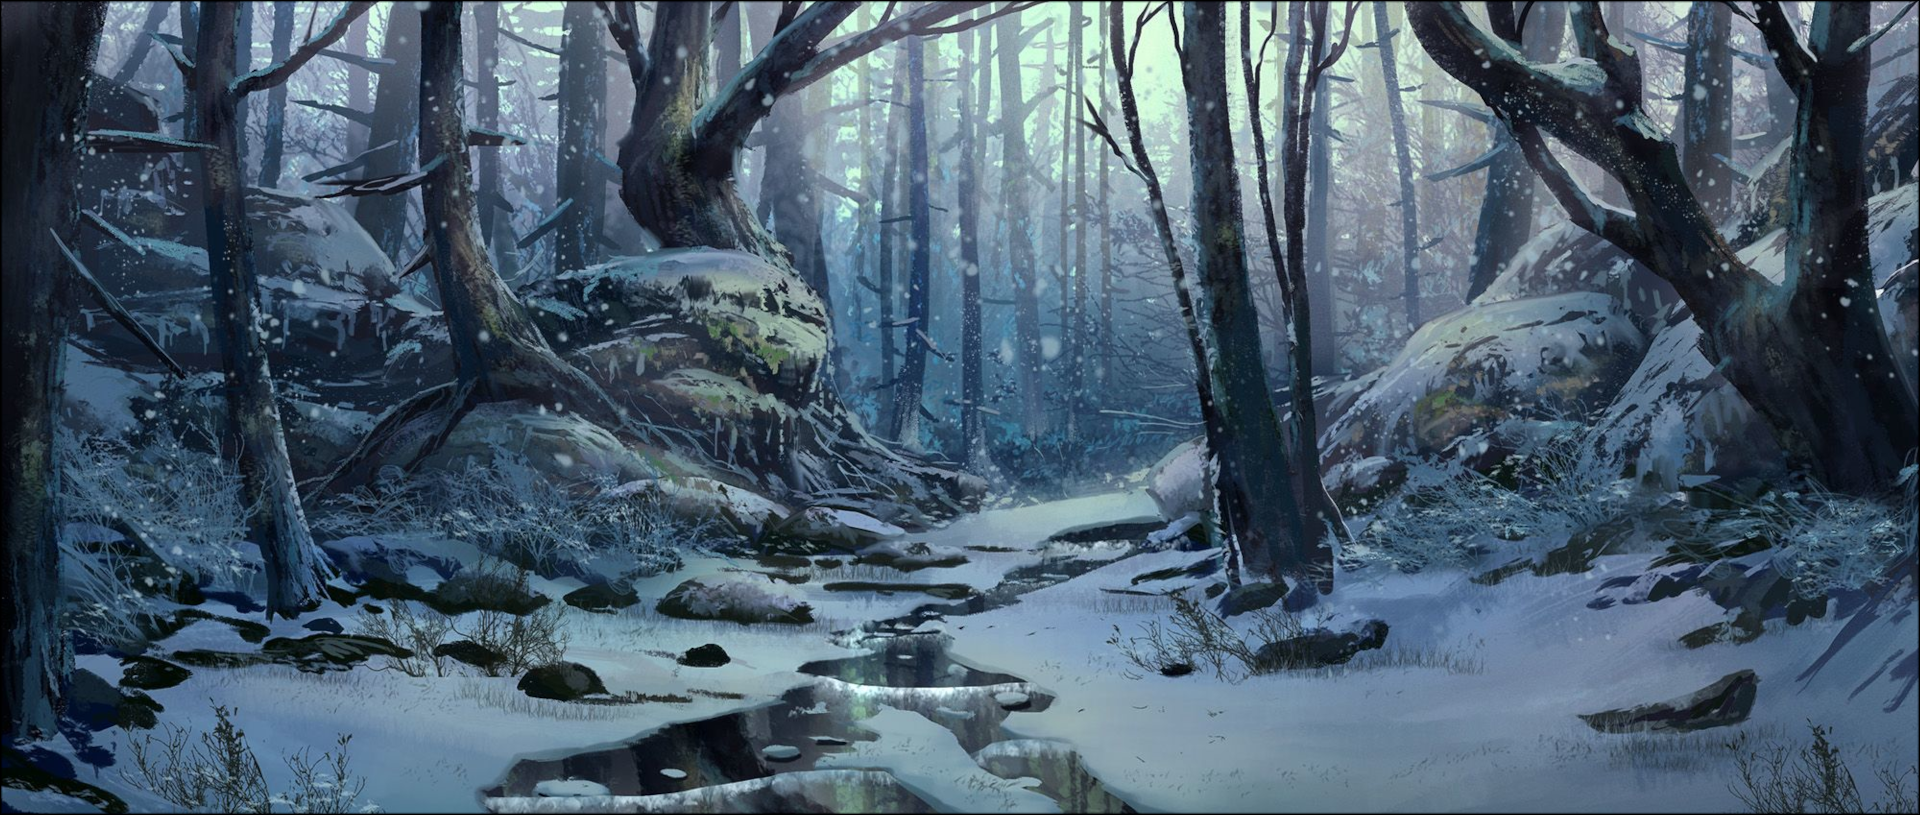
\includegraphics[width=0.95\textwidth]{01yuadrem/img/11tallwoods.png} \
        \centering \large{\textbf{The Tallwoods}}
    \end{DndTable}
\end{table*}

\subsection*{Northern Territories} \label{ssec::northernterritories}
The northmost region of Yuadrem, the Northern Territories are comprised by the Whitenorth, the Red Islands, the Tallwoods, the Blank Fields, and the Sulfur Lake.
The region is split by the Wall of Ice and Stone, a colossal mountain range that spans from coast to coast.

North of the wall is Whitenorth, an area split between the ancient ird kingdom of Krudzal and the territorial giants of Jatuunsa.
Its few inhabitants are beings of extreme resilience and fierceness, acclimated to the harsh habitat.
First among these are the giants, mountain-sized creature of stone, ever locked in war with Krudzal.

The middle of the region is characterized by the endless mists.
The area coincides with the north pole, and is inexplicably warm and misty despite its location.

To the west of Whitenorth is the Red Fjord, named so by its most common tree, the red maple.
The are is regarded sacred by the Krudzalians, who believe it to be the resting place of the sun god, Jua\~nanisz.
The fjord is currently occupied by Ribinhep, a uman nation ever standing up against the northerner irds.

Below the Wall of Ice and Stone are the Tallwoods and the Blank Fields.
The Tallwoods are an association of pine and redwood forest, using the mountains to hide from the cold winds.
The forests are devoid of civilized life, and the stone trolls who inhabit them make sure that they stay that way.

The Blank Fields are a vast, freezing tundra.
The low temperatures and strong winds in the area prohibit the growth of any vegetation.

The west of the fields are known as the Wurmlands, and they are solely inhabited by wurms.
Wurms are large reptile-like creatures that attack all foolish enough to approach their subterranean colonies.
The eastern portion of the land is filled to the brim with a variety of bughna gat tribes, ever in conflict for the large reserves of copper and coal in the mountains.

East to the fields is the Arctic Archipelago.
This cluster of islands separate the Whaler's Sea from the frigid ocean up north.
Mostly bare and desolate, the islets equally house ird, gat, uman, and zaloth settlements.

The strongest force in the archipelago is the Kaldrathal nation.
Having the only vessels strong enough to withstand the ship-sinking idzels, they regulate commerce in the entire archipelago.
% idzels or idzelal are inspired on Illhevi (https://abookofcreatures.com/category/iceland/page/2/).

% !TEX root = ../main.tex

% \begin{table*}[b]%
%     \begin{DndTable}[width=\linewidth]{X}
%         \centering
%         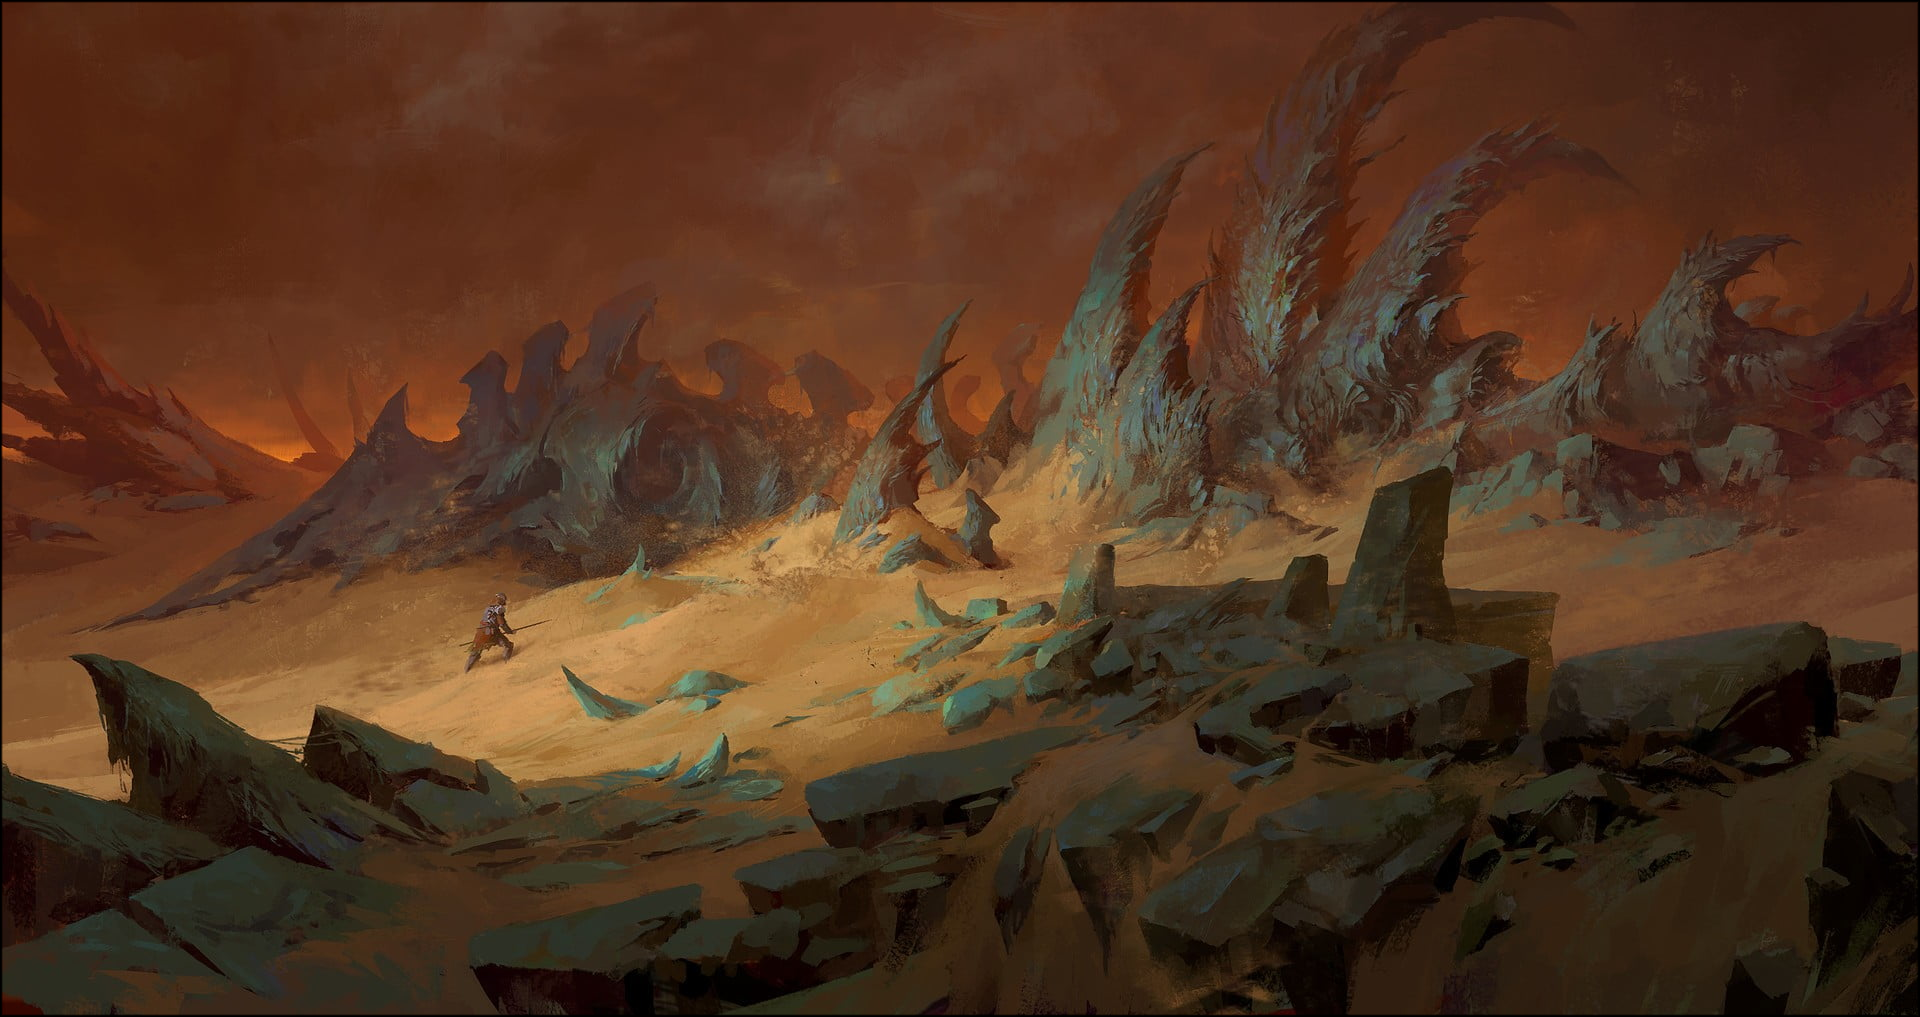
\includegraphics[width=0.95\textwidth]{01yuadrem/img/12dead_sea.png} \
%         \centering \large{\textbf{The Bone Cliffs of the Dead Sea}}
%     \end{DndTable}
% \end{table*}

\subsection*{The Three Deserts} \label{ssec::threedeserts}
Effectively splitting Yuadrem in half are the three deserts: Zoedrem, Zashlath, and the Dead Sea.

Zoedrem is a large expanse of yellow sands the embraces the waves of both the Whaler's Sea and the Teal Ocean.
The desert runs undisturbed from the Sulfur Lake down to the Defiled River.
It is commonly regarded as the most forgiving of the three deserts.

More fearsome than the sands are its inhabitants, the five dratl ird houses of Zoedrem.
Descendants of the fallen empire of Hulnar, they hide their settlements along the stone cliffs.
They are constantly in search of prey, robbing and murdering any traveler foolish enough to travel in their territories.

At the easternmost point of Zoedrem is the Sylvan Canyon, the only area in the desert able to host life.
The gorge is the home of the independent nation of Viphoger.
Apart from its inhabitants, the canyon's soil has rich natural deposits of oil, salt, and gemstones.
These resources grant Viphoger a strong economy despite its young age.

Southeast of Zoedrem and across the Ichor Mountains lie the Dead Sea, an artificial desert created by the tall kin's folly.
The desert's sands are of a sickly gray color, and any creature that inhabit the land for too long suffer particular mutations.
Its inhabitants, the treb gats and the cursed umans are perhaps the best examples of this.

The sands become blacker the more you approach the spire, the largest mountain in Yuadrem.
The et city of Jan'krug stands atop it, where the ritual that caused the Schism took place.
A long chasm divides the eastern region of the Dead Sea, remnants of the passage of the breathing island, Cabb Goem-Rlamesh.
Surrounded by hill, mountain, and river, the desert naturally prohibits passage to it, almost as if it's protecting a twisted secret.

Apart from the kins that call this desert home, the Dead Sea is infested with other monstrosities.
These are categorized into two: The Nyxborn and the children of Cabb.
The former are giant insect-like creatures that can be as large as an elephant and as precise as a mosquito.
The latter are tormented amalgamates that dislodged from Cabb Goem-Rlamesh, ever haunted by insatiable hunger and unending pain.

% Along with the tortles, grungs, and umans, the Schism brought forth terrible creatures known as the Nyxborn.
% These insect-like monstrosities can be as huge as the Mirmekolon, a colossal ant-lion hybrid, or as precise as the Khanokoladtes, a palm-sized moth that pierces skulls with its sharp dart-like mouth.

South, through the Hammerfall canyon, is the Zashlath desert, the driest of the three.
Featureless and white, only the hardy sunstruck oths have been able to call the desert home, and even they are wise enough to only establish by the neighboring mountains.

Zashlath practically receives no precipitation, and its white-colored sands reflect the scorching sunlight to deadly effect.
Truth is the desert remains largely unexplored to this date, and only rumors exist about the horrors that might hide among its sands.
Famous among these is the Haimorrois, a red horned snake whose bite forces the blood out of one's body.

% !TEX root = ../main.tex

\begin{figure}[t]
    \centering
    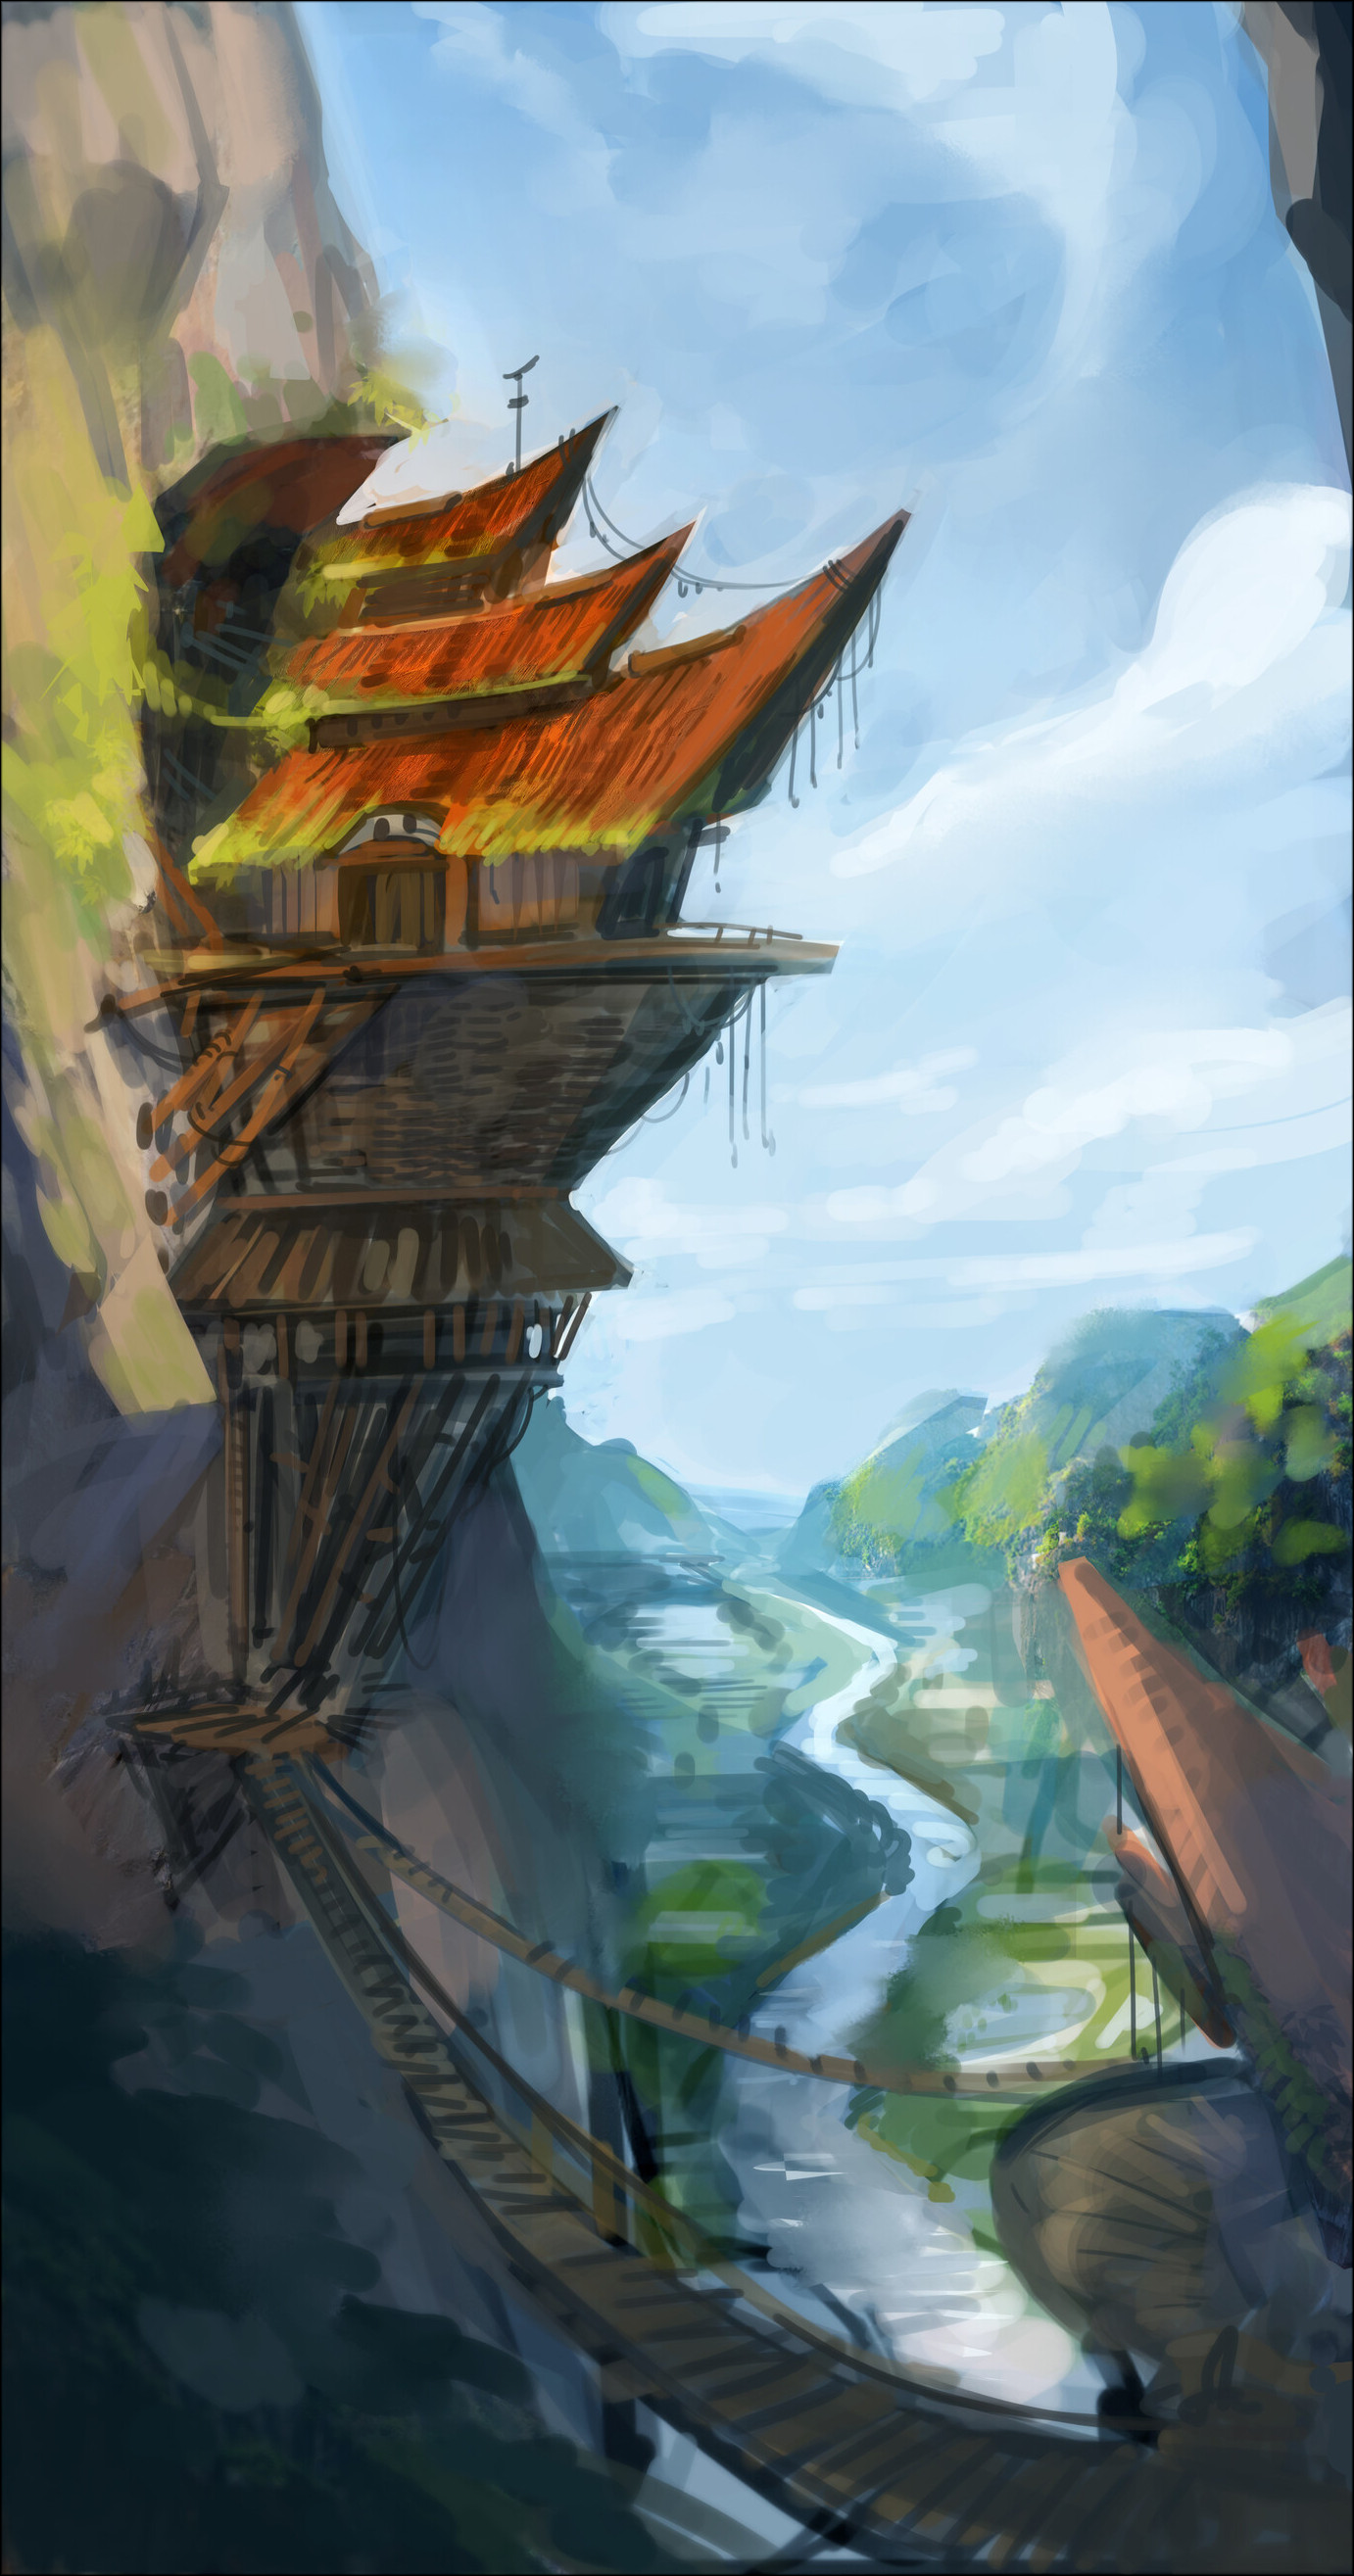
\includegraphics[width=0.46\textwidth]{01yuadrem/img/13siszgoel.png}
    \caption*{\centering \large{\textbf{Siszgoel, Kaldrathal's Capital}}} % TODO: Check if I can change the font of the caption
\end{figure}

\subsection*{Whaler's Sea} \label{ssec::whalerssea}

% intro
The cradle of modern civilization, the Whaler's Sea is home to both well-established and blooming countries.
Its coasts protected from harsh winds by mountain ranges and its cold waters supplied with both whale and idzel, the region couldn't be a better location to develop the modern world.
Idzels are large whale-like creatures known for their ship-sinking fury and their large supply of the valuable ambergris, the main ingredient in artificial qualars.

% Krejek and Kaljek
Sitting at the middle of the sea are the two southernmost islands of the Arctic Archipelago, Krejek and Kaljek.
The first is a large island covered by mountains, rocks plains, and deciduous forests.
It serves as the mainland for the independent nation of Kaldrathal.
%, who competes with Sulia as the main exporter of nitrate.

Starting out as a Krudzalian colony, they merged the quench-hardened steel of the thulkraka irds with their natural supply of nitrate.
This combination produces resilient steel firearms, including cannons, muskets, and flintlock handguns.
They remain the only exporter of these valuable weapons.

Kaljek, the smaller of the two islands, is a desolate land, with only few pine and birch forests.
It is separated by four nations inhabited by gat and ird alike.
While historically peaceful towards each other, they have recently been divided by conflict, all over the recently discovered gold veins that hide under their land.
% 661 AS: gold veins found under the ground.

% southern coast
South of both islands are the Horned Shores and the Fesh Peninsula.
The first is known for its calm, dry mediterranean climate, its sparse forests, and the great concrete gat city-states that rise from its ground.
Most of the land is devoid of natural resources, with scarce mines and low-quality wood.

% eastern coasts
East to these lands is the Fesh peninsula, an area inhabited mainly by gats, tortles and thulkraka irds.
A humid subtropical climate permeates the cape, and it is known for its harsh, capricious waters and frequent storms.
Also well-known are the tortles inhabiting the small island of Mbeat, for it is the only place where they have met safety after their arrival in Yuadrem.

In both regions lie the oldest nations of Yuadrem, the Seven kingdoms of the Sea.
Historically renowned raiders and pillagers, they are now famous for their passivity --- focusing on enterprise and artisanship.
What they offer is their expert craftgatship, and among them are the only bonecarvers capable of manufacturing qualars.

% western coast
Finally, to the west of Krejek one can find the two daughters of Palegna, the countries of Sulia and Drer.
The two nations were in a sense ``commisioned'' by the oth nation of Palegna.
Sulia was born to control the worrying growth of the Sulfur Lake, and Drer to restrict the growth of the bughna gat tribes of the Blank Fields.
% Both countries also served as an experiment of sorts for the word-obsessed oths, since the official language in both nations is the artificial Standard Language created by them.

Sulia benefited greatly from what would originally be their burden, and have developed a refined industry based on sulfur.
Their sulfur-based fertilizer is the basis of modern agriculture, their fiery blackpowder is only matched by Kaldrathal's, and their self-preserving wines are a taste craved all around the continent.
% They also have great sulfur-inlaid furniture!

Drer, in stark contrast with its sister, is a nation whose economy solely depends on pillage.
Re-imagining Sulia's blackpowder, they use their fire-bearing weapons to push back and raid their northern neighbors.

% !TEX root = ../main.tex
\subsection*{Beryl Sea} \label{ssec::berylsea}

The Beryl Sea is a searing, tropical region, ever battered by violent winds and waters.
The region is tapered in rainforests, and it houses two of the largest nations in Yuadrem: the warring Jenkashian empire and the mysterious Gannag.
The coasts see few other countries, and seldom do ships sail in these lands.
% Apart from the two, the coasts are also inhabited by a somewhat limited variety of countries, including the ancient Edede, the resilient Voskferm, and the strange Na'ane.

% Drejeck
Westernmost of Yuadrem is the thick, dark, and moist jungle of Drejeck.
Drejeck is the birthplace of the savage naenks and the ceremonial tsaneks, and is now entirely occupied by their nation, Gannag.
Despite being born even before the Schism, the beings of Gannag are primitive and untamed, and keep their tribal ways despite regular contact with more sophisticated cultures.
The jungle is also inhabited by large and dangerous beasts that threaten the unprepared explorer, like the aggressive nadubis or the silent whowie.
% And the bulettes and the Yara-ma-yha-who.

% Fog Gorge
East to Drejeck is the Fog Gorge, a well-forested canyon island ever enveloped in fog.
While primitive, the tribes of Gannag are far from free-living, and are bound by strong shackles to their superiors.
While naenks are used to this hierarchical system, many of the more intelligent tsaneks grow tired of it over time.
A hundred and fifty years ago, a group of tsaneks went as far as to establish their own independent tribe of Na'ane in the misty island, abandoning their brethren in favor of an unrestrained lifestyle.
Freely they carry on with their ceremonies and rituals, protected from their neighbors by mist and stone.

% Qul archipelago
Further east one finds the Qul archipelago, a clump of islands that collectively served as the birth bed of the Jenkashian empire.
Jenkash is a coalition of tribes that only managed to unite after cutting down the last tree in their mountainous islands.
This led to an explosive expansion of their empire, and they swiftly conquered the neighboring lands.
Their territories now span most of the coasts of the Beryl Sea.

The archipelago itself is absolutely desolate, with barely any tree or foliage growing atop its igneous rock.
Perhaps the only bright side of this uncontrolled deforestation is the fact that it brought to light the iron and diamond veins in the eastern side of the archipelago.
These resources are heavily exploited by the qulbaba irds, and led to their signature diamond daggers.

% Dratl'fal savanna
North of the archipelago is the Dratl'fal savanna, occupied entirely by Jenkash.
The only plant that freely grows in the savanna is bafarmat, a purple moss covering its entire southeastern coast.
This plant is the primary food source of the cavernous species that live under the ichor mountains.
Its spread has allowed the hornbeetles to move into the area, a strong species of giant blue beetles that served as companions to the now ruined nation of Phrisht.

In oldentimes, the dry lands served as the birth bed for many gat city-states, of which only Dzorvepem and Jorea remain standing, now part of Jenkash.
Despite its lack of resources, the whole area was sought after by the now divided empire of Hulnar, who battled against the blooming nation of Phrisht for more than 300 years for it.
This everlasting conflict was only stopped by Jenkash, who in their thirst for conquest ended up dissolving the untiring countries.

% \begin{figure}[t]
%     \centering
%     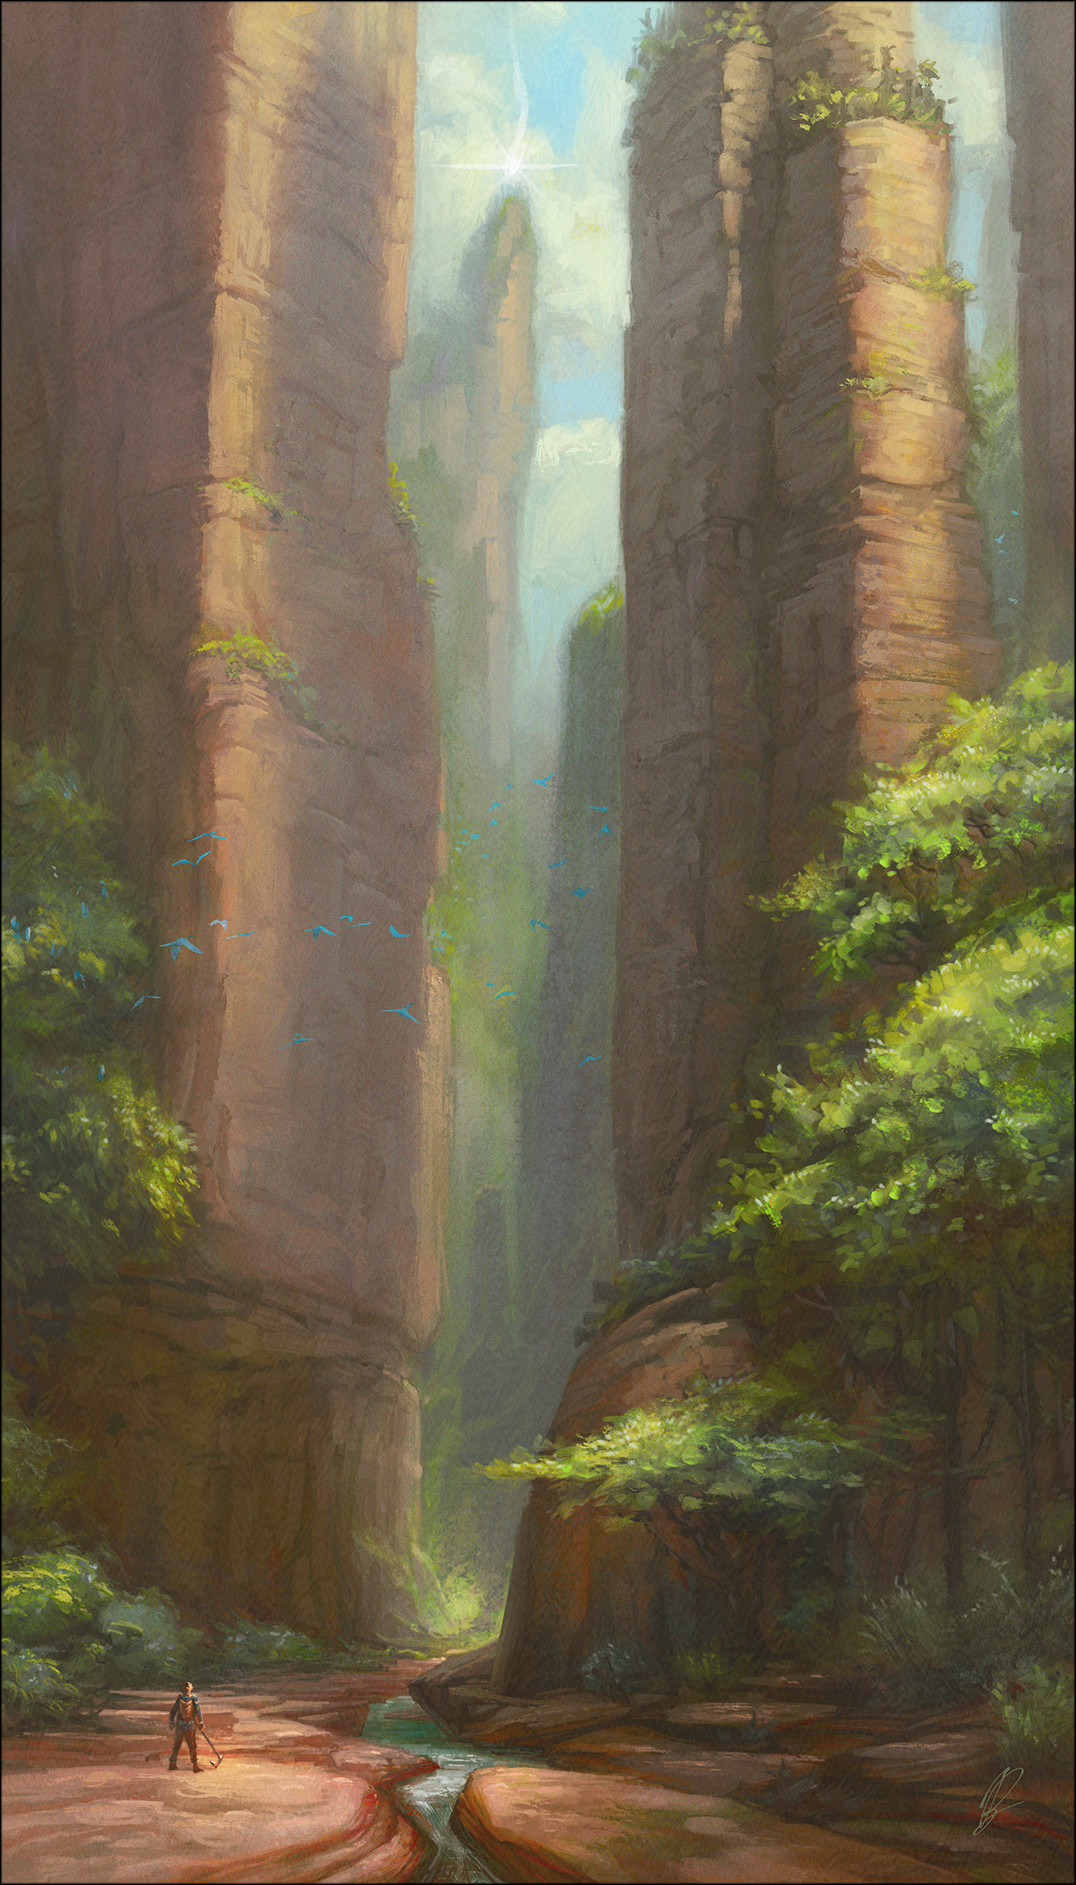
\includegraphics[width=0.46\textwidth]{01yuadrem/img/14fog_gorge.png}
%     \caption*{\centering \large{\textbf{The Fog Gorge}}}
% \end{figure}

% Ironlakes Island & Zashlath savanna
Moving to the easternmost portion of the sea one can find the Ironlakes Island and the Zashlath savanna.
The former is a large island full of forests and lakes.
It was historically a part of the peaceful marset nation of Edede, but most of it now belongs to the warring empire.
The Zashlath savanna is the area west of the desert, protected from its dry air by the moisture of the cerulean waters.

% !TEX root = ../main.tex

\begin{table*}[b]%
    \begin{DndTable}[width=\linewidth]{X}
        \centering
        \includegraphics[width=0.98\textwidth]{01yuadrem/img/15om.png} \
        \centering \large{\textbf{Om, Isken's Capital}}
    \end{DndTable}
\end{table*}

\subsection*{Barbaric Territories} \label{ssec::barbaricterritories}

To the east of Yuadrem are the Barbaric Territories, a region defined by the brutality of war and the greed of an empire.
From north to south, the land can be divided into five areas, each with its own distinct characteristics: the Drylands, Cabb Goem-Rlamesh, the Shield Sea, the Chirping Wilds, and the Xuam Peninsula.

% Drylands
Northernmost are the Drylands, a field devoid of trees or any sort of tall flora.
The area is plain and parched, dried over the years for its lack of rains or rivers.
The northernmost area of the savanna remains bare to date, and is the most tortuous stretch between the Fesh Peninsula and the southern nations.

% Mzavit river and southern savanna
Down across the Mzavit River, the savanna becomes humid and with this water comes civilization.
A wide array of gat city-states have been established here.
Able to withstand the thunderous force of the Jenkashian and Iskenese armies and the hulking chimeras from the Next, these states are noteworthy for their fortitude.
Of special note is the adamant country of Byurev, who have halted the growth of Isken for almost three centuries.

% Cabb Goem-Rlamesh
% NOTE: In the whole island of Cabb Goem-Rlamesh a faint crying sound can be heard.
Off the coast of the Drylands lies a place known as the breathing island, Cabb Goem-Rlamesh.
A harrowing immensity, the landmass is constructed entirely of flesh and bone, and is believed to be what remains of the ets.
Not much is known about the island, and none of the few explorers who have travelled to it retain their sanity.
The mad tell tales of a mortifying city of flesh, and of strange, shape-shifting inhabitants.

% Shield Sea & The Nest
% Wrong information - geomancy was invented by an ancient civilization that warred with the tall kin eons ago, but was erased from history by the victors. There are ruins from this civilization at the basin of the lake, and Fo is the last remaining member from it.
Southwest of the Drylands rest the Shield Sea, an enormous body of water fed by a wide array of tributaries from the Forking Peaks.
In antiquity, the ruined ird civilization of Hairuus invented the art of geomancy in its coasts, raising from the basin the island of ``The Nest'' at its center.
The island currently hosts only one being, Fo.
Fo is a strange creature, rumored to be out of this world.
It welcomes visitors with a variety of fierce chimeras.

% Chirping Wilds
Southeast from the Drylands and passing through the Do Nana swamp are the Chirping Wilds, a vast and largely untamed rainforest.
The jungle is inhabited only by the Iskenese empire, a large grung nation that expelled the original ird and marset population.
The only territories currently not held by the grungs' military might are the strong qulbaba irds of Harual to the west, and the marsets of Uzuz from the Xuam peninsula.

The Xuam Peninsula is the southermost point of the Barbaric Territories, and is located just south of the Grasping Gulf.
The region has facilitated the development of Uzuz due to the heavy presence of wurmroot, a white-leaf poplar tree that is conveniently toxic to all foreigner kins, specially to grungs.

% !TEX root = ../main.tex

% \begin{table*}[t]%
%     \begin{DndTable}[width=\linewidth]{X}
%         \centering
%         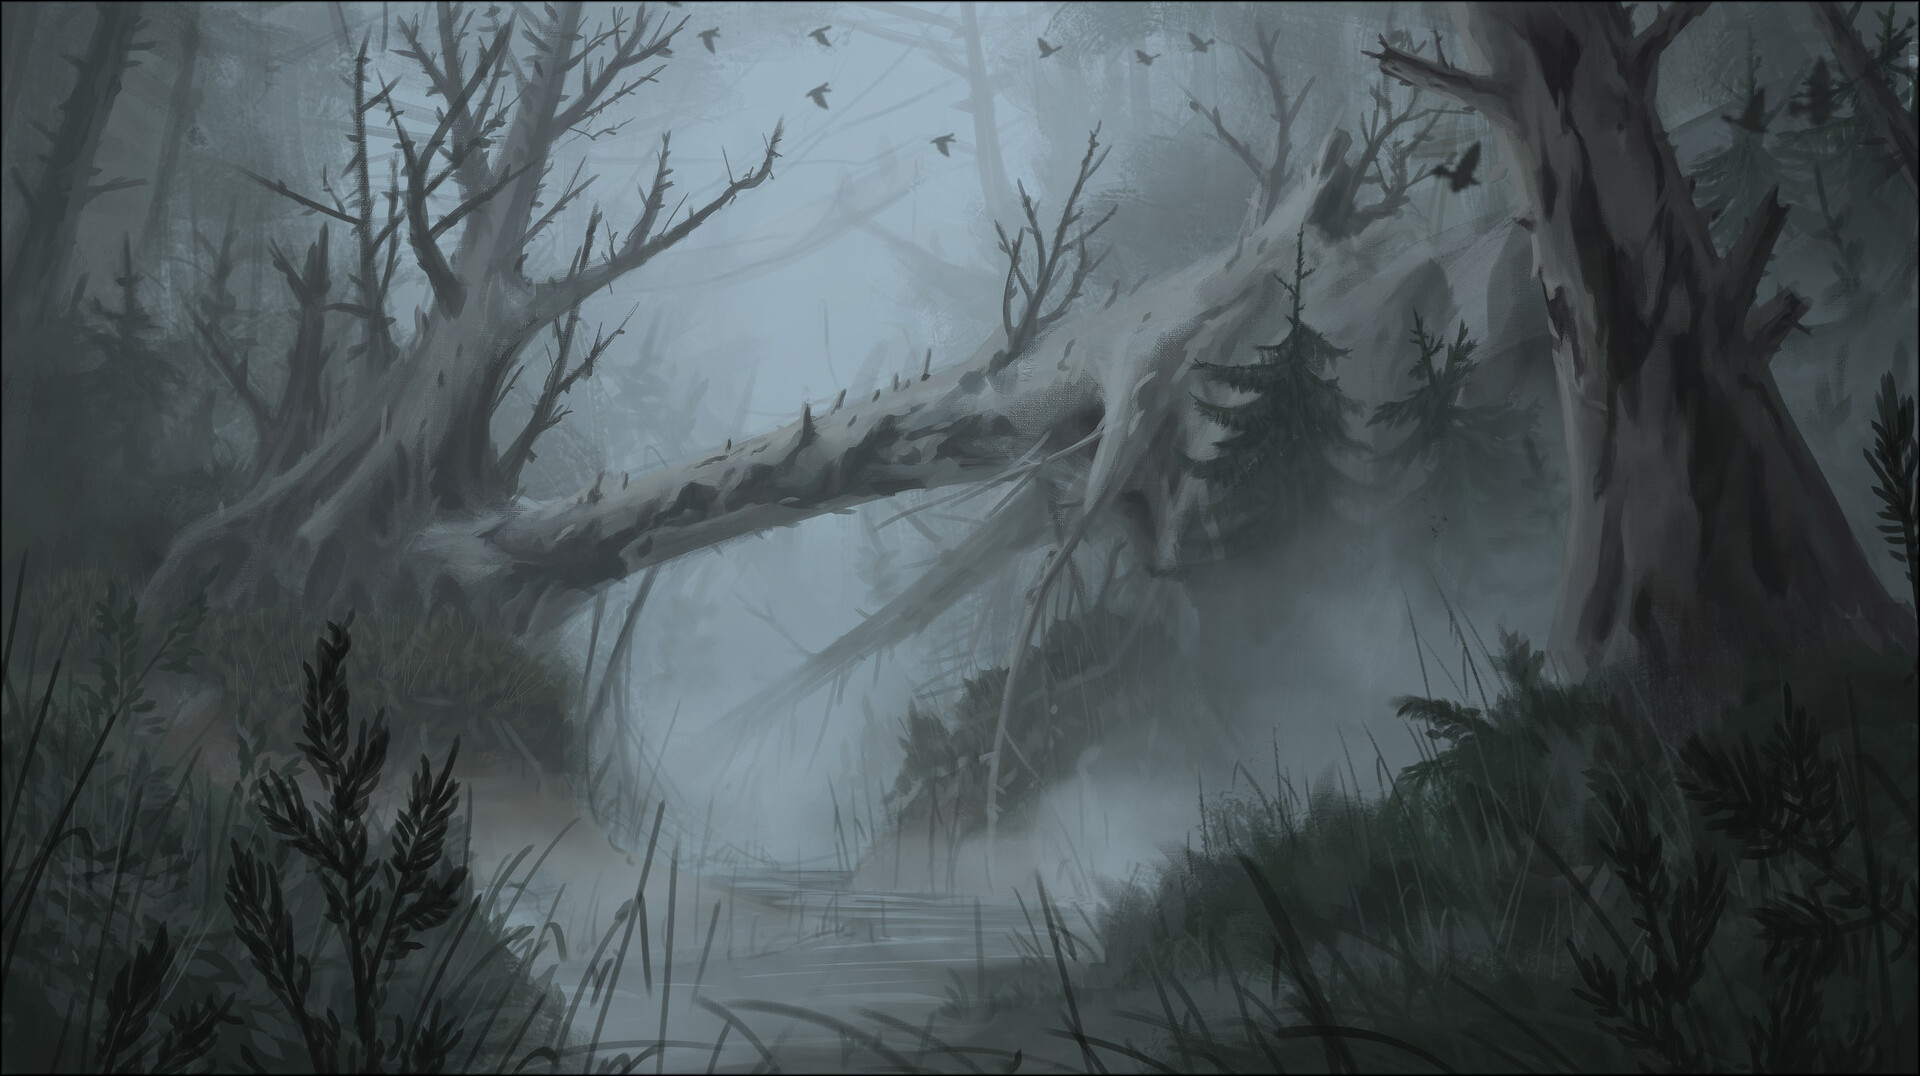
\includegraphics[width=0.98\textwidth]{01yuadrem/img/16pale_blemish.png} \
%         \centering \large{\textbf{Forests Surrounding the Pale Blemish}}
%     \end{DndTable}
% \end{table*}

\subsection*{Wildlands} \label{ssec::wildlands}

% intro
The southernmost region of Yuadrem is aptly named the Wildlands, for it is a large expanse of untamed fields, forests, and lakes.
Starting at the bottom-most part of the forking peaks, the area has seen very little intervention from the civilized world.
This is attributed to the fact that the Wildlands are infested with both deadly creatures and strange tide-altering illnesses.

% Savage Plains
Just below the forking peaks and the Beal river is the northmost point of the Wildlands, the Savage Plains.
They are a humid subtropical area covered by marshes and plains, with few patches of forest in-between.
Fed by many rivers from the mountains, the lands define the southern territories of the Iskenese empire, expanding thorough the whole region.

However, Isken's grip on the Savage Plains is tenuous at best, as the region is as much controlled by the grungs as it is by the local wildlife.
Just as in the forest below, a great variety of foul beasts and creatures can be found in these swamps.
Of special note among these are the giant mole-like jinshus, beasts unique to region who suffocate the unprepared by sinking them beneath the earth.

% Everwoods
As dangerous as these plains are the Everwoods, the forest that grows south of them.
This ancient woodland used to be a place of respite after the harsh swamps, but all that swiftly changed about 400 years ago.
In an attempt to manipulate the tides, the Rashiist school of thought from Ignelli summoned The Sorrow into Yuadrem.
The Sorrow is an entity of unknown origin, who seeped into Yuadrem due to the Rashiists folly.
On arrival, it swiftly slayed all members of the school of thought, and brought fourth with it strange creatures and diseases that now plague the once peaceful forest.
This event came to be known as the Tidal Sway.

% Pale Blemish
Not only bringing forth pain and disease, the Tidal Sway also ravaged the land around Ignelli, area now known as the pale blemish.
All flora was destroyed, and the ground turned into badlands.
The field now serves as a grim reminder to all of the dangers of manipulating the tides.

Despite the destruction, the scholars from the Igneist school continue to work in their temple, studying the tides and The Sorrow.
Perhaps one day they'll achieve their goal and undo their sister school's sins, expelling the Sorrow and healing their lands.

% Niknek Peninsula
West of the Everwoods is the Niknek peninsula, a thin, elongated stretch of land filled with volcanoes and gorges.
The cape was spared from most of the effects of the Tidal Sway.
Niknek and the nearby Vuvu Isles now house the refuge marsets from the Ironlakes Island.

% Elderberry Wilds
At the southern tip of Yuadrem are the Elderberry Wilds and the Ironwoods, a set of pine and spruce forest surrounding the Manta Sea.
The area is partly occupied by Gronselar, an old and forgotten colony of Krudzal.
% Not much is known about these forests due to their remote location.
% Not much is known about the area due to its remote location, but even here a semblance of civilization exists. in the form of the ird nation of Gronselar, and the regions of Froibias, Glameas, and Visilias.


% !TEX root = ../main.tex
\section{Cultures} \label{sec::cultures}

\DndDropCapLine{U}{pon their abandonment, the kins were}
quick to travel to the far reaches of Yuadrem, carrying civilization with them.
Over the years, languages, religions, and rites of different natures spreaded far and wide to create the complex network of cultures we see today.

% !TEX root = ../main.tex
\subsection*{Religions} \label{ssec::religions}

\DndDropCapLine{R}{eligion is an important part of life}
of the many cultures of Yuadrem.
Some worship specific pantheons of gods, others praise unpersonified concepts, and a selected few worship nature itself.
% In the times before the schism there was a wide belief that the tall kin could answer prayers, but their worship is now forbidden in most of the continent.

% The true existence of these divinities is a widely discussed subject, but their worship is undeniable.
From the nature-worshiping folk of Jenkash to the god-birds of Krudzal, each culture performs a set of rituals in the name of their deities, and some even claim to be able to channel their divine power.
While it might be hard to pinpoint the exact number of religions in Yuadrem, a few are built into the fabric of civilizations, and are easy to tell apart.

\subsubsection{Igneism}
The oth scholars hailing from Ignelli were the first to conceptualize the tides.
They learned that the tides are intrinsically woven into sentience.
As tightly tied threads between sentient creatures, a change in the tidal alignment in one has profound effects in that of those nearby.
% Each tide was then assosiated with a symbol and an entity, to give a more concrete face to it and facilitate its worship.

The blue tide is represented by a blue unfinished book, representing the eternal pursuit of knowledge.
The gold tide is symbolized as a seed or an egg, telling of the coming of future life with proper nourishment.
Indicated by a torch, the indigo tide tells of the truth revealed under light, and the punishment exerted upon those who hide it.
A broken compass represents the red tide, representing the roaming of those who walk without roads.
The silver tide's symbol is a bell, denoting the attention obtained by those who seek fame.

Nearing the year 174 AS, the knowledge of the tides split the Ignelli school in two - The Igneists and the Rashiists.
% The Zelseists, who simply sought to further understand this new discovery, and the Rashiists, who attempted to wield and manipulate them.
The latter created a system of magic known as Rashid, with which they could potentiate the tidal alignment of others.
Despite the warnings issued by their sister school, the Rashiists honed their craft to its maximal potency, and suffered severely from it.
Their actions awoke a strange an antique and mysterious creature: The Sorrow.

% The Sorrow is a being of indescribable shape who was summoned to Yuadrem by the Rashiists' folly.
Breaking the mind of any who lay their eyes upon it, it swiftly took the lives of all who corrupted the balance of the tides, thus ending the Rashiist school's folly.
Its presence caused the pale blemish, and with it came horrid creatures known now as the xuagra.
Seeing the destruction caused by their sister school, the Igenists hid the knowledge of their former brethren, forbidding Rashid in any shape or form.
% Finally, they changed their own name to Igneists in an attempt to bury the other school in anonymity.

Igneism is the worship of the tides as a concept, and the active pursuit of keeping the five balanced.
Igneists recognize that sentience cannot exist without the tides, and praise them as thanks for the capacity of independent thought.

\subsubsection{Tanethism}
Across the long history of the Seven Kingdoms, varied deities were gradually associated with many different concepts, and any gat would pray to different gods at different times and circumstances.
For example, one might say a prayer to the Traveler for luck, make an offering to Tamaz before going to the market, and pray to appease Matevos when a severe storm blows in --- all in the same day.

Independent to any institution, the gat scholar Taneth officially published ``The Rituals and Gods of the Gats'' in 511 AS.
The book was an exhaustive compilation of the more than a thousand deities that were praised by the different kins of the Seven Kingdoms, and proposed a reduced pantheon of 15, distilling the chaotic pantheon into the main gods.
Taneth's work was barely known during their life, and they died without due recognition.

Later, in the year 577 AS, the king of Khedrat Olag the Immortal sought a method to reduce the religious disparity among their people.
Either by divine will or happenstance, they came upon this book by Taneth, and established Tanethism as the official religion of Khedrat, imitating the well-established creed of other nations.
By command of the government, many churches were erected in the name of each god, and the many gods of the gats coalesced into a more sober pantheon of 15.

Many have a favorite among the gods, one whose ideals and teaching they make their own.
A few even dedicate entirely to a single deity, serving as a priest, acolyte, or champion of that god's image.
Famous among these devout beings are the nimrod, an organization of zealous hunters of Phusinhe who pursue all who disturb the balance of Yuadrem.
Well-known as well are the followers of Havetish, a group of gats in golden robes whose goal is to distribute wealth and food to the impoverished hamlets of the inner regions of the Seven Kingdoms.

\begin{table*}[b]%
    \begin{DndTable}[width=\linewidth, header=The Gods of Yuadrem]{p{2cm}p{0.8cm}p{3cm}p{1.8cm}X}
        \textbf{Name} & \textbf{Tides} & \textbf{Domains} & \textbf{Religion} & \textbf{Symbol} \\
        The Scholar  & B  & Reason, Knowledge     & Igneism   & A many-armed blue oth reading multiple books. \\
        The Zealous  & R  & Passion, Zeal         & Igneism   & A red dratl ird standing over a sand dune. \\
        The Star     & S  & Admiration, Fame      & Igneism   & A naked tall one, sometimes replaced by a shadow or a uman. \\
        The Equalist & I  & Justice, Equity       & Igneism   & An indigo gat holding a spear and a coin. \\
        The Altruist & G  & Empathy, Compassion   & Igneism   & A furtive golden marset carrying a basket full of eggs. \\
        The Sorrow   & -  & Balance, Punishment   & Igneism   & An indistinct cloaked figure holding a bloody heart. \\
        Changing God & -  & Secrecy, Manipulation & Rashiism  & A robed oth with a featureless bronze mask. \\
        Febrid       & B  & Intellect, Wood       & Tanethism & A gat forming a crescent moon with its horns. \\
        The Traveler & BR & Luck, Beer            & Tanethism & An indistinct figure cloaked in light brown robes. \\
        Vugar        & BG & Family, Fertility     & Tanethism & A gat prince dressed in a simple silver toga. \\
        Vahagn       & R  & Mountains, Fire       & Tanethism & A red quies holding a colossal mace. \\
        Genadi       & RI & Bravery, Love         & Tanethism & A grung warrior carrying a sword and a lute. \\
        Sakris       & RS & Fun, Wine             & Tanethism & A uman servant carrying cups and wine. \\
        Matevos      & S  & Glory, Water          & Tanethism & An ice zaloth holding a bident and a shield. \\
        Hanutsh      & SB & Teaching, Books       & Tanethism & A tsanek dressed in scrolls and paper. \\
        Tamaz        & SG & Wealth, Silver        & Tanethism & A gray ird eternally flying towards the sun. \\
        Phusinhe     & I  & The Stars, Metal      & Tanethism & A giant tortle with the visage of stars in its shell. \\
        Nadzim       & IB & Justice, the Sky      & Tanethism & A purple oth holding an abacus and a spyglass. \\
        Gathoz       & IS & Secrecy, Murder       & Tanethism & A kinless being with shifting body and face. \\
        Bagrat       & G  & Farming, Earth        & Tanethism & A gat farmer with tools made of gold. \\
        Havetish     & GI & Leadership, Tyranny   & Tanethism & A naenk holding a golden and an indigo spear. \\
        Mziva        & GR & Self Sacrifice        & Tanethism & A blonde marset with a flowered back. \\
        Jua\~nansiz  & G  & Day, Sunlight         & Tsalemism & A rainbow-colored heron followed by northern lights. \\
        Dzadsiz      & R  & Night, Darkness       & Tsalemism & A black raven surrounded by never-dispersing mists. \\
        The Observer & -  & Cosmos, the Unknown   & Cosmism   & A titanic three-eyed slug ridden with tentacles and appendages.
    \end{DndTable}
\end{table*}

\subsubsection{Tsalemism}
It is indubitable that astral concepts are commonly associated to divinities, and no religion reflects this as clearly as Tsalemism.
Tsalemism is a belief that originally gained popularity in the coasts of Krudzal, quickly becoming the official religion of the nation and of many thulkraka irds.
Due to its proximity to the north pole, Krudzal experiences long polar days and nights every year, and this irregular schedule naturally led to the personification of night and day.

Day is associated to Jua\~nansiz, a rainbow-colored heron that brings daylight and colors to the entirety of the polar region.
Jua\~nansiz eternally hunts Dzadsiz, a black raven who in turn seeks to tire the heron and finally feast on its exhausted body.
The birds' duel is unending, and the wreckage of their battle is used to explain the chaotic fjords in the Northern Territories.

The boreal lights seen near the pole are Jua\~nansiz's trail.
The mountainous landscape of the Whitenorth are the places where Dzadsiz fell, struck by the heron.
% The endless mists were created by the raven in an attempt to hide from Jua\~nansiz.
These and many other natural phenomena of the Northern Territories are explained by the birds and their eternal duel.

The two birds are not worshiped equally, but their wrath is feared by all.
A sailor may produce a small temple to appease Dzadsiz before sailing, and a cartographer may sing a praise to Jua\~nansiz before taking flight.

\subsubsection{Cosmism}
While the worship of the tall ones is forbidden, their own religious ideas persist in the form of Cosmism.
Cosmism is related to the search of one's place in the larger scheme of things, dubbed the ``cosmos''.
The Observer is the manifestation of the elusive concept of this cosmos, an omnipresent god observing all of Yuadrem at once.

The ideas behind the doctrine were originally conceived by the ets in time immemorial, and cosmists are generally met with disdain and criticism.
Due to this, many acolytes of the religion practice their rituals in the protection of the darkness, and it's very rare to see a church openly dedicated to cosmism.

Cosmism explains some of the strange phenomena of Yuadrem as the whims and thoughts of The Observer.
The tides are the reactions of The Observer to the actions of each being.
Qualars are the medium by which people can commune with The Observer, granting them some of Their wisdom.

% Cosmists fear the cosmos, and carry strange and surreptitious rituals to appease The Observer or gain its favor.

However, what may be shunned in the surface can always find its place underground.
There seems to be a deep connection between the search of oneself in the larger scheme of things and the ego death experienced in the tsanek melds.
Many temples and ritual places exist in the mushroom cities of the cave-dwelling fungal kin, and cosmism is the official religion of the tsanek nation of Na'ane.
% Tsaneks view the cosmos with curiosity, and seek to understanding through observation and hypotheses.

% !TEX root = ../main.tex
\subsection{Languages} \label{ssec::languages}

\begin{table*}[b]%
    \begin{DndTable}[width=\linewidth]{X}
        \centering
        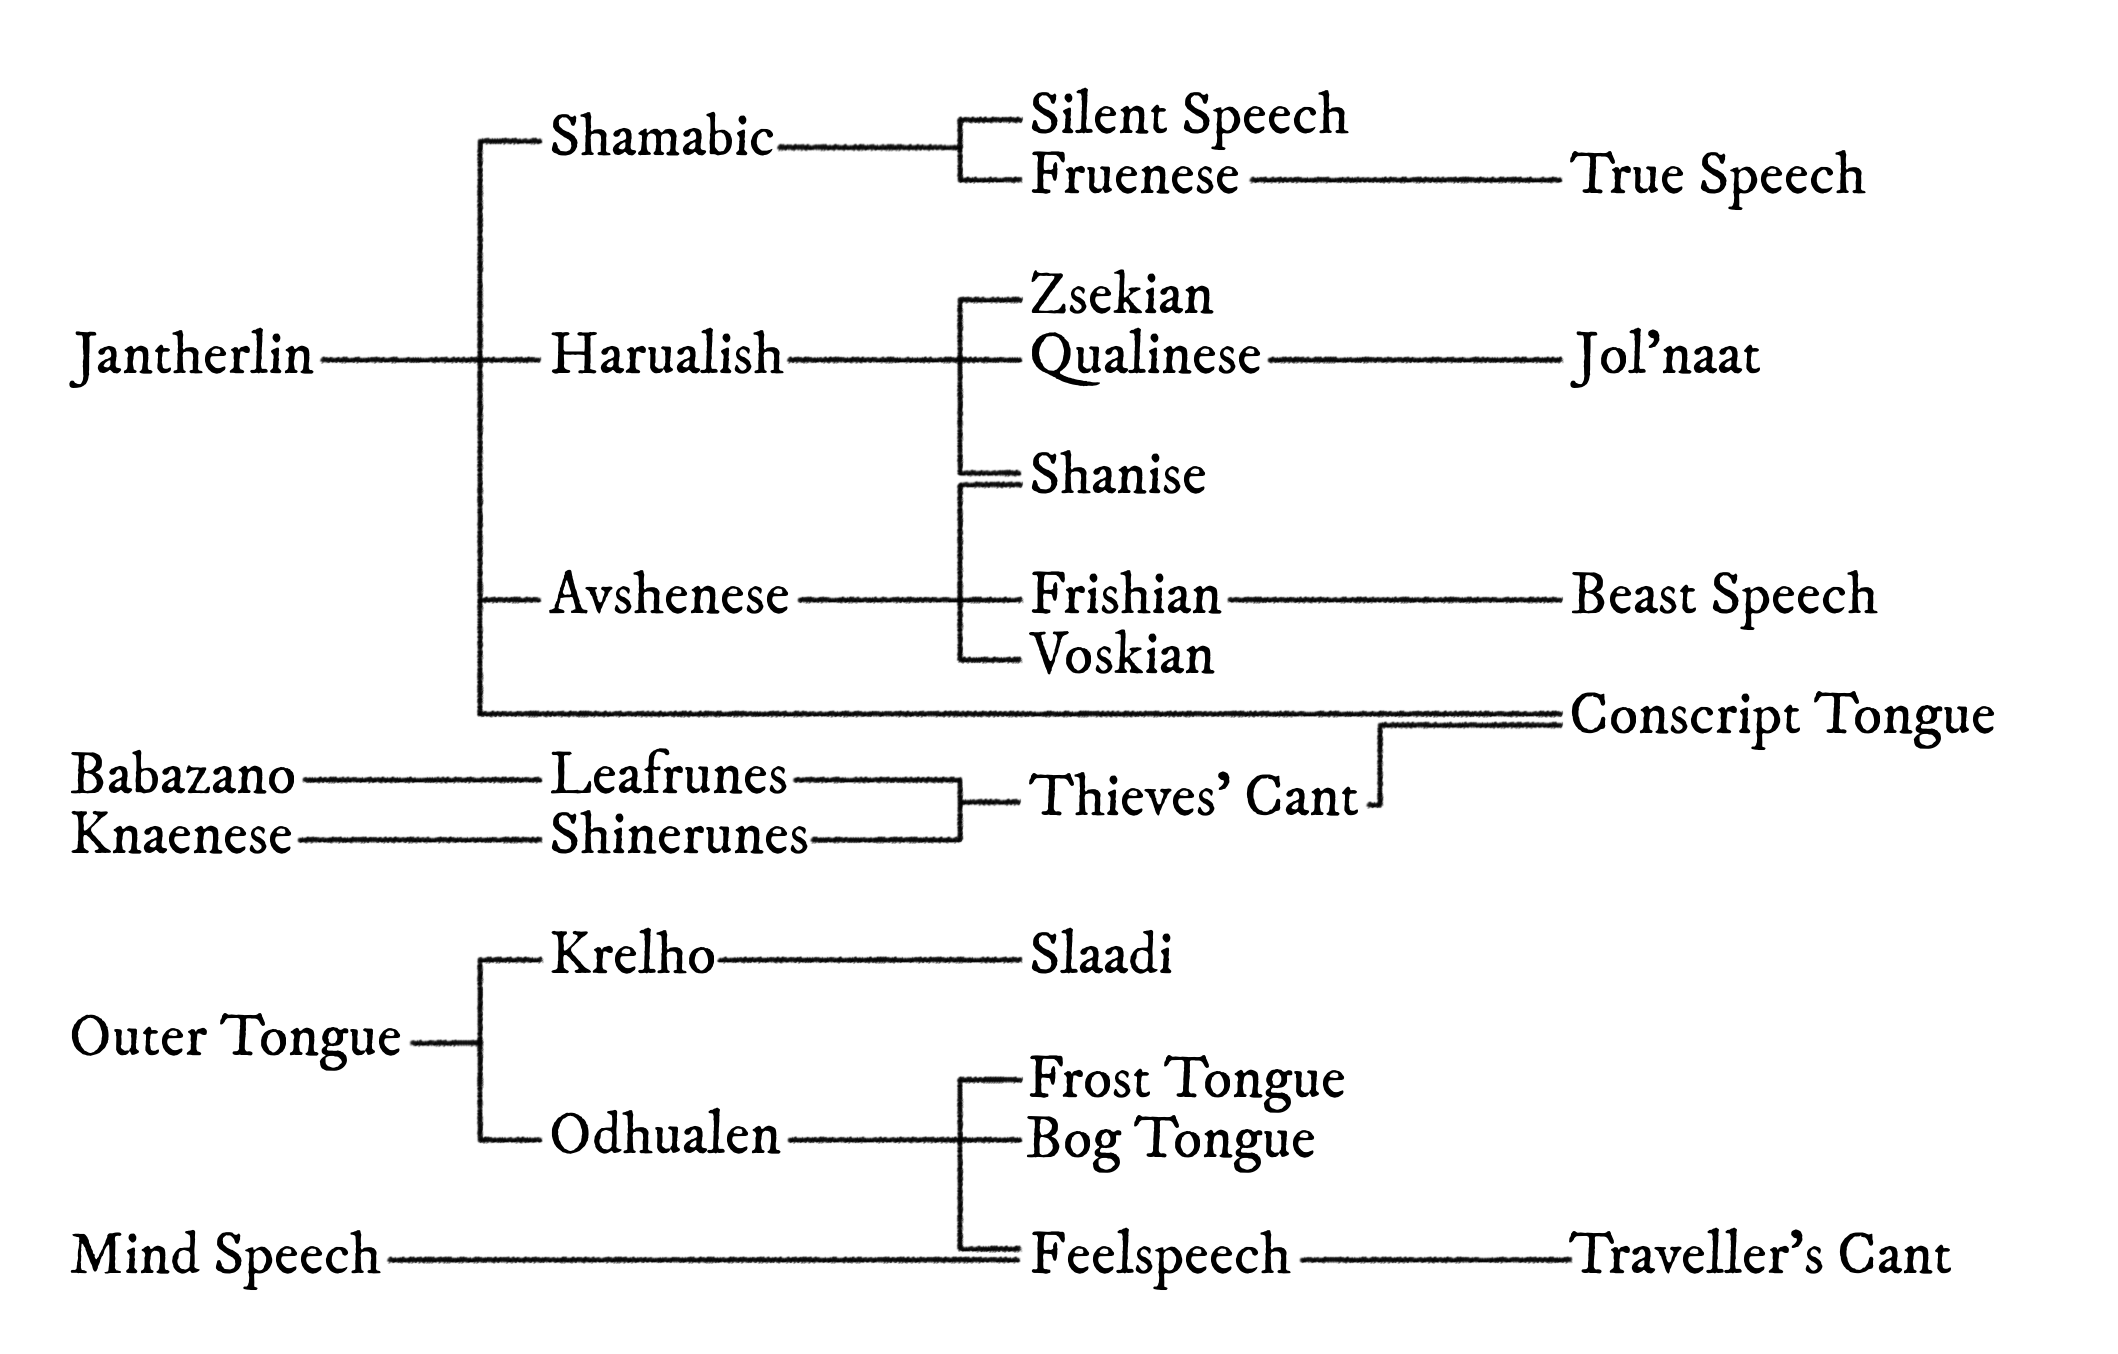
\includegraphics[width=0.99\textwidth]{01yuadrem/img/22languages_map.png}
    \end{DndTable}
\end{table*}

A great variety of languages permeate Yuadrem, both of natural spawn and artificial design.
While it is impossible to identify each tongue and its variations, many efforts have been done over the years to classify the common ones.

Based on lexical and grammatical similarities, languages are separated into four generations, and five distinct families.
The following tables classify these languages, pointing to their script and original speakers.

% As is discussed in the following pages, your country of origin determines your language more than your kin.
% Despite this, some languages are indeed associated to certain kins, as they were the original speakers.

\begin{DndTable}[width=\linewidth, header=First Generation]{p{2.6cm}p{2.6cm}p{2cm}}
    \textbf{Language}  & \textbf{Original Speakers} & \textbf{Script} \\
    Jantherlin         & Ets                        & Varies \\
    Babazano           & Marsets                    & - \\
    Knaenese           & Naenks \& Tsaneks          & Knaenese \\
    Outer Tongue       & -                          & Outer Tongue \\
    Mind Speech        & Zaloths                    & -
\end{DndTable}

\begin{DndTable}[width=\linewidth, header=Second Generation]{p{2.6cm}p{2.6cm}p{2cm}}
    \textbf{Language}  & \textbf{Original Speakers} & \textbf{Script} \\
    Shamabic           & Oths                       & Shamabic \\
    Harualish          & Irds                       & Harualish \\
    Avshenese          & Gats                       & Avshenese \\
    Leafrunes          & Marsets                    & Leafrunes \\
    Shinerunes         & Naenks \& Tsaneks          & Shinerunes \\
    Seedspeech         & Gannagian Tsaneks          & - \\
    Krelho             & Tortles \& Grungs          & Krelho \\
    Odhualen           & Umans                      & Outer Tongue
\end{DndTable}

\begin{DndTable}[width=\linewidth, header=Third Generation]{p{2.6cm}p{3.2cm}p{2.2cm}}
    \textbf{Language}  & \textbf{Original Speakers} & \textbf{Script} \\
    Silent Speech      & Oths                       & - \\
    Fruenese           & Sulian Oths                & Fruenese \\
    Zsekian            & Zsek Irds                  & Harualish \\
    Qualinese          & Jenkashian Irds            & Harualish \\
    Shanise            & Northern Irds \& Gats      & Shanise \\
    Frishian           & Jorea \& Dzorvepem         & Avshenese \\
    Voskian            & Voskferm \& Voskgrit       & Avshenese \\
    Thieves' Cant      & Rogues \& Thieves          & Thieves' Cant \\
    Slaadi             & Slaads                     & Krelho \\
    Feelspeech         & Zaloths \& Umans           & -
\end{DndTable}

\begin{DndTable}[width=\linewidth, header=Fourth Generation]{p{2.6cm}p{3.2cm}p{2.2cm}}
    \textbf{Language}  & \textbf{Original Speakers} & \textbf{Script} \\
    True Speech        & Palegna \& Sulia           & - \\
    Jol'naat           & Jenkash                    & - \\
    Beast Speech       & Jorea                      & - \\
    Conscript Tongue   & Cabb Goem-Rlamesh          & - \\
    Traveller's Cant   & Zaloths \& Umans           & Traveller's Cant
\end{DndTable}

% \subsubsection{First Generation}
% \paragraph{Old Tongue} A very complicated and intricate language spoken by the tall kin, the original settlers of Yuadrem.
% It's spoken form involves various complex articulations and the definition of a word can vary greatly based on the context.
% Additionally, each tall one had their own personal version of the written form, and others would understand it as much as they understood the individual.
% % This makes the reading of the old tongue extremely difficult for the kin that remain in the world, since understanding a particular tall one's scribbles essentially requires understanding their own version of the language.
% % Nowadays, only scholars and archaeologists understand the language, and it is not normally used anywhere.
% \paragraph{Marset Tongue} Every marset is already able to speak this strange, repetitive language.
% The marset tongue only has ten consonants, and ten verbs.
% % The rest of their vocabulary is built up from there, making their language very difficult to speak or understand by kins other than the marsets.
% Marset tongue can be spoken in one of two ways: soundlessly, through lip reading, or screamed as loud as possible, with no middle ground.
% The language cannot be written down.
% \paragraph{Naenk Tongue} Short words and strong consonants define the naenk tongue.
% Lacking lips and teeth, naenks make heavy use of their alveolar ridge and hard palate to produce syllables.
% The written form of the language involves carving lines and holes onto bark or stone.
% \paragraph{Outer Tongue}
% \paragraph{Mind Speech}

% \subsubsection{Second Generation}
% \paragraph{Dust Tongue}
% \paragraph{Ird Tongue}
% \paragraph{Gat Tongue}
% \paragraph{Leafrunes} Very easy to learn, but kept secret by the archer kin.
% A marset will teach this set of runes only to creatures that it deeply trusts, and only if it's strictly necessary.
% Ten leafrunes exist, all of which are used individually and to convey very simple meaning.
% % \textit{colony}, \textit{danger}, \textit{fun place}, \textit{hiding spot}, \textit{observation point}, \textit{predators}, \textit{road}, \textit{sacred place}, \textit{source of food}, and \textit{source of materials}.
% \paragraph{Shinerunes}
% \paragraph{Krelho}
% \paragraph{Nomad Tongue}

% \subsubsection{Third Generation}
% \paragraph{Silent Speech}
% \paragraph{Standard Language}
% \paragraph{Zsek Tongue}
% \paragraph{Qul Tongue}
% \paragraph{North Tongue}
% \paragraph{Beetle Tongue}
% \paragraph{Gilded Tongue}
% \paragraph{Thieves' Cant}
% \paragraph{Slaadi}
% \paragraph{Frost Tongue}
% \paragraph{Bog Tongue}
% \paragraph{Feelspeech}

% \subsubsection{Fourth Generation}
% \paragraph{True Speech}
% \paragraph{Jol'naat}
% \paragraph{Beast Speech}
% \paragraph{Conscript Language}
% \paragraph{Traveller's Cant}

% !TEX root = ../main.tex
\subsection*{Schools of Magic} \label{ssec::schoolsofmagic}
% TODO. The whole magic system is being updated. See to it that this subsection reflects that.

\subsubsection{Bonereading\\ \small{Mevthan}}
Long before Tanethism became the official religion of Khedrat, the art of bonereading was already a common practice among its populace.
By using the bones of marine creatures as catalysts, witch doctors of antique were able to listen to the wisdom of their divinities.
After hearing the plights of the common gats, the gods could influence events to help - or punish - those who deserved it, and witch doctors were of high regard in society thanks to this ability.

As the art developed over time, new spells and incantations have appeared.
The bones are now used for more than divination, but as ways to directly influence the reader's surroundings in more direct manners.
Nowadays, bonereading remains an important part of Khedrat's culture, and is still practiced both by the farmer to ask for a good harvest, by the sailor to attain a safe voyage, and by priests exert the gods' will.

% Some maintain the argument that bonereading is not a form of communication with the gods, but that the magic lies in the bones themselves.
% Such words fall on deaf ears in the common gat, and are considered heresy by the church, punishable by exile.

\begin{table*}[b]%
    \begin{DndTable}[width=\linewidth]{X}
        \centering
        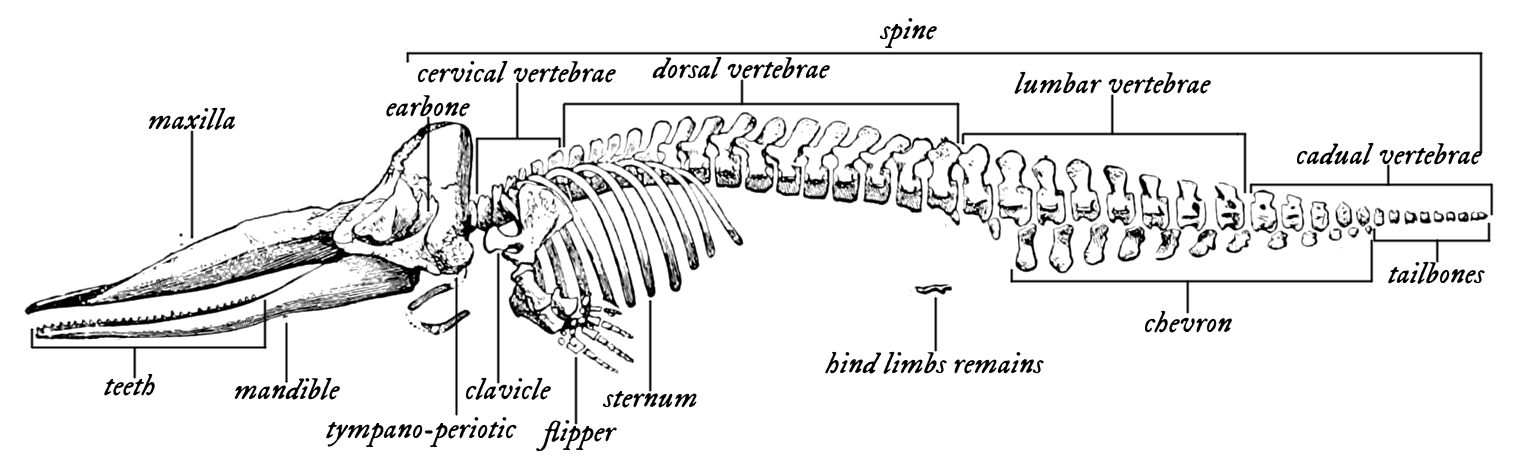
\includegraphics[width=0.99\textwidth]{01yuadrem/img/23sperm_whale_skeleton.png}
    \end{DndTable}
\end{table*}

\subsubsection{Wordbinding\\ \small{Dremshamad}}
Well known is the obsession of the many houses of Palegna with words, names, and languages, and evidence of this is wordbinding.
Wordbinding, or Dremshamad in dust tongue, is the art of giving strength to words so that, no matter the medium, their mere utterance conveys an tangible effect in the world.
Its spells are many and varied, like saving effects in scrolls or books to be invoked later, binding the will of creatures by using their true names, and speaking command words that can't be disobeyed by any mean.

Perhaps the most meaningful product of wordbinding are reflexive contracts.
These agreements bind through the strength of words alone, enforcing their terms upon the signing parties by tying harsh effects to the rights and duties specified.
Always produced in triplicate with each requiring three signatures per party, reflexive contracts are practically unvoidable, thus regarded as the perfect mean to ensure cooperation between beings, houses, or even entire nations.

% Crafting a document with words of power:
% * List of effects that can be produced (more are unlocked as expertise increases)
% * Interaction with words that produce such effect (spoken out loud, whispered, listened to, read)

% All contracts must have a clause that can void the contract by design. Most usually it is being burned by the fire of a wyrm, since this act is neigh impossible without dying.

\subsubsection{Windherding\\ \small{Dentrala}}
Perilous are the winds from the southern ocean, relentlessly tearing apart any ship that dares sail it's turbulent waters.
Many forget that the many tribes from the Qul archipelago had to deal with these strong winds and storms in their daily lives.
To face this, they slowly developed a complex system of sympathetic magic.

By standing atop large poles within eyesight of each other, ird witches from the dentralin tribe managed to stop the wind simply by holding their breath.
This practice gave rise to a wide array of wind-based spells that the tribe wise to use to their advantage during the tunsal wars, and eventually led to the establishing of Jenkash.

\subsubsection{Sigaldry\\ \small{Guen Tsue}}
Unlike other languages, the naenk tongue is deeply rooted in nature itself, and can be used to even directly talk to it, with seedspeech being the clear example.
This quality of the language led to Gannag's shamans to develop a writing system that can evoke effects when interacted with, called shinerunes.

The tsaneks of Gannag use this method to create self-triggering traps, which are set about villages to catch prey and ward off would-be invaders.
Apart from this, intricate shinerunes are used to many different effects, such as a silent bell alerting of the presence of a stranger in a dwelling, a self-heating plate to boil water in, or clothes that spontaneously heat up as a reaction to bad weather.
Truly, the capabilities of shinerunes are only limited by the creativity and skill of their author.

\begin{table*}[t]%
    \begin{DndTable}[width=\linewidth, header=\centering Knaenese Alphabet]{X}
        \centering
        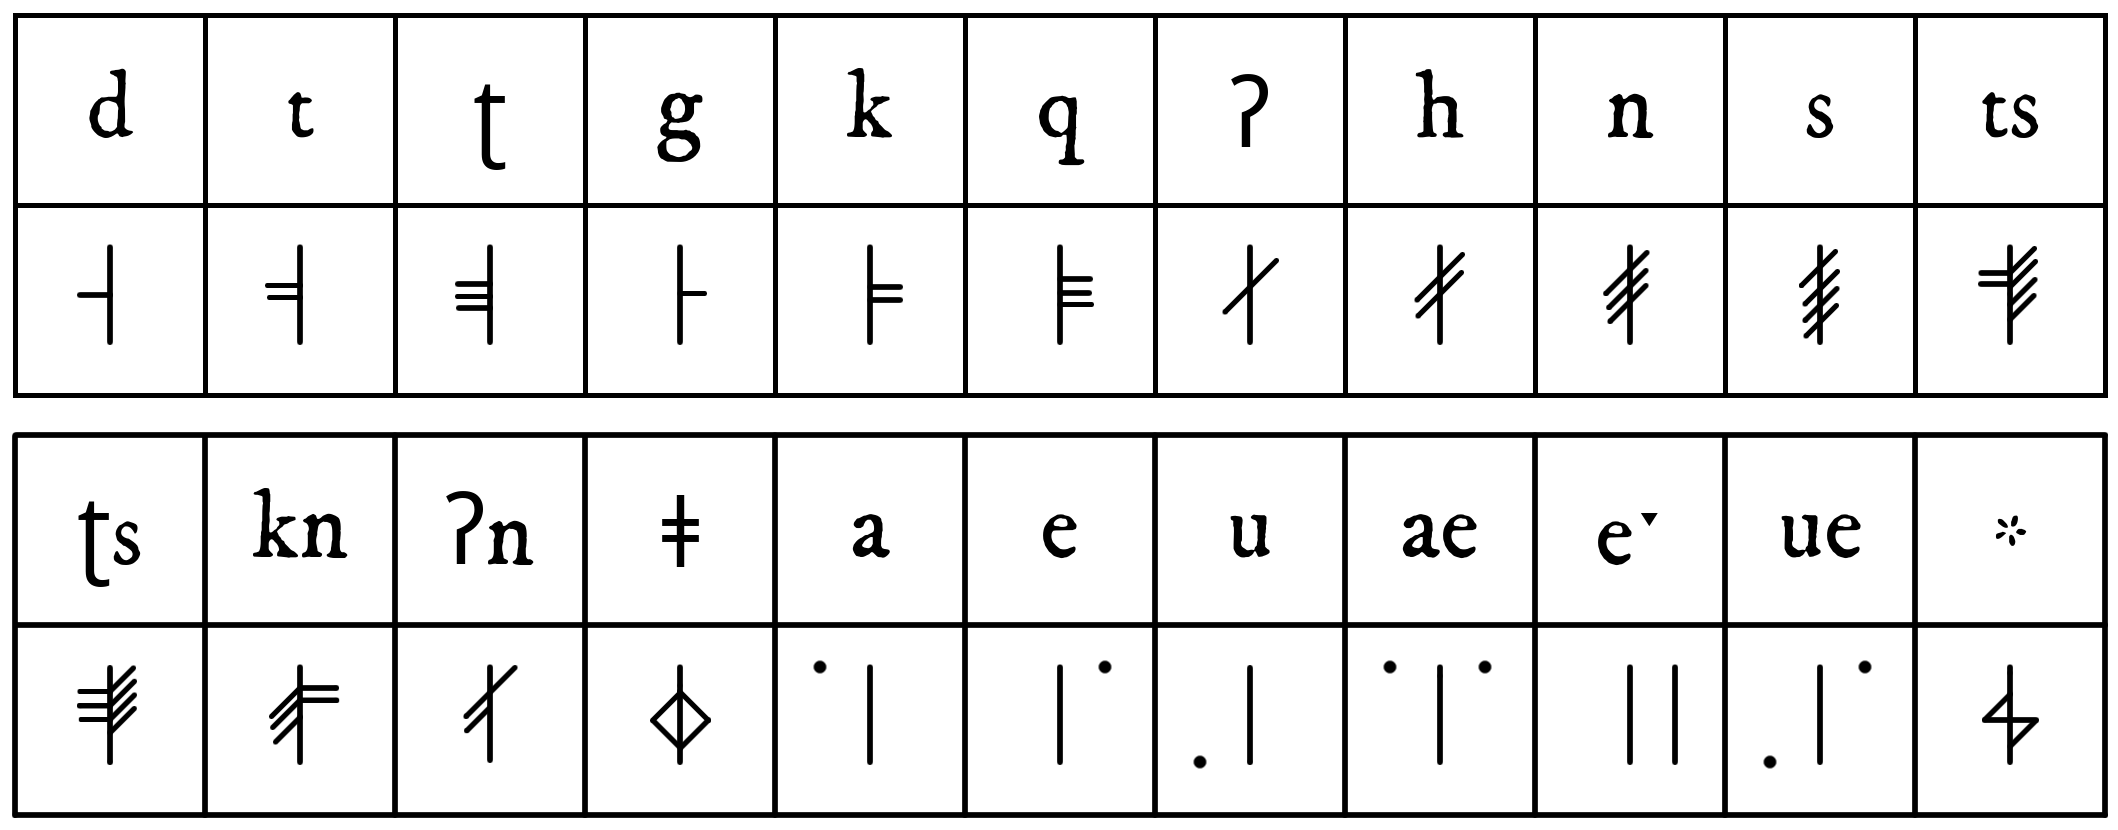
\includegraphics[width=0.99\textwidth]{01yuadrem/img/23knaenese_sample.png}
    \end{DndTable}
\end{table*}

\subsubsection{Psionics} % NOTE. I don't like the name but it's not that bad I guess.
Perhaps the strangest part of the zaloths is the fact that they do not speak through a mouth, but directly into other beings' minds.
This ability is only made possible by the special nature of the zaloths themselves, and is very rarely seen in the other kins, in peculiar gifted individuals.
Not limited to telepathy however, the art developed into a plethora of mind-based abilities known as psionics.

Psionics are fueled by one's own mind without external sources of energy, meaning that the art exerts a great effort from the author.
The zaloths have elaborated varied psionic effects to date, expanding their original telepathy to more tangible effects, like clairvoyance, telepathy, and many mind-altering effects.

\subsubsection{Similarity Sympathy}
% Blink (quantum teleport): Cantrip to teleport, only usable if being perceived by no sentient being when moving to an area not perceived by any sentient being. Hard to use in most cases yet extremely powerful in certain scenarios. (Mechanically it's a cantrip but using it is actually tiring, so it can't really be used as a reliable method of transportation).
% The best thaumaturges are blind FUCK YES!!

No one can deny that Yuadrem completely changed after the schism.
The ash storm ravaged the land and caused the 9 year famine, tens of thousands of strange creatures poured in, and new, alien kins settled into the land.
For better or for worse, the event transformed the fabric of reality.
Soon after the schism the witches and shamans of the early world started to experiment with a new and strange form of magic: the Similarity Link.

This link is a strange form of sorcery which seems to follow different rules than the other schools.
It affects directly the physical properties of objects and creatures, like making rocks weight as little as feathers, or changing the size of other creatures.
Perhaps the strangest part of this is that it seems to behave differently depending on if it's being perceived or not.%, and thaumaturges take advantage of this by covering their eyes when casting certain spells.

\subsubsection{Tidal Manipulation\\ \small{Rashid}} % !!
Rashid involves manipulating the tides in the air or in others to attain one's goals.
Originally taught by the sole survivor of the Rashiist school of thought, it ranges from simple charms and illusions to potent spells with effects that vary depending on the caster's or target's tidal alignment.

Every Rashid user knows that they must exercise their magic in secrecy, since the practice is severely punished due to Rashiism's dark history.
The most experienced in the art however know that the one they truly have to fear is the Sorrow.
The Sorrow is the being that destroyed the Rashiist school of thought, leaving the pale blemish as a warning to any who dares follow their teachings.

\subsubsection{Fleshshaping\\ \small{Cthai'khas}} % !!
Recently reborn in the breathing city of Cabb Goem-Rlamesh is the almost lost art of Ukarilth: fleshshaping.
An everyday act of the tall kin, fleshshaping is a kind of magic that involves transfiguring the flesh of the caster or of others nearby, be them alive or dead.

While most fleshshapers remain in their putrid island, some have started to show up in the eastern parts of Yuadrem, and the art is slowly being spread by concealed mages.
A strange attribute of fleshshaping that sets it apart from the other schools is that its effect vary depending on the species of the caster.
For example, while a gat can mold its flesh to temporarily use its bones as weapons, a naenk can grow roots into the floor to catch prey, and a quies can reinforce its wooden exterior in preparation for an attack.


% !TEX root = ../main.tex
\begin{figure}[H]
    \centering 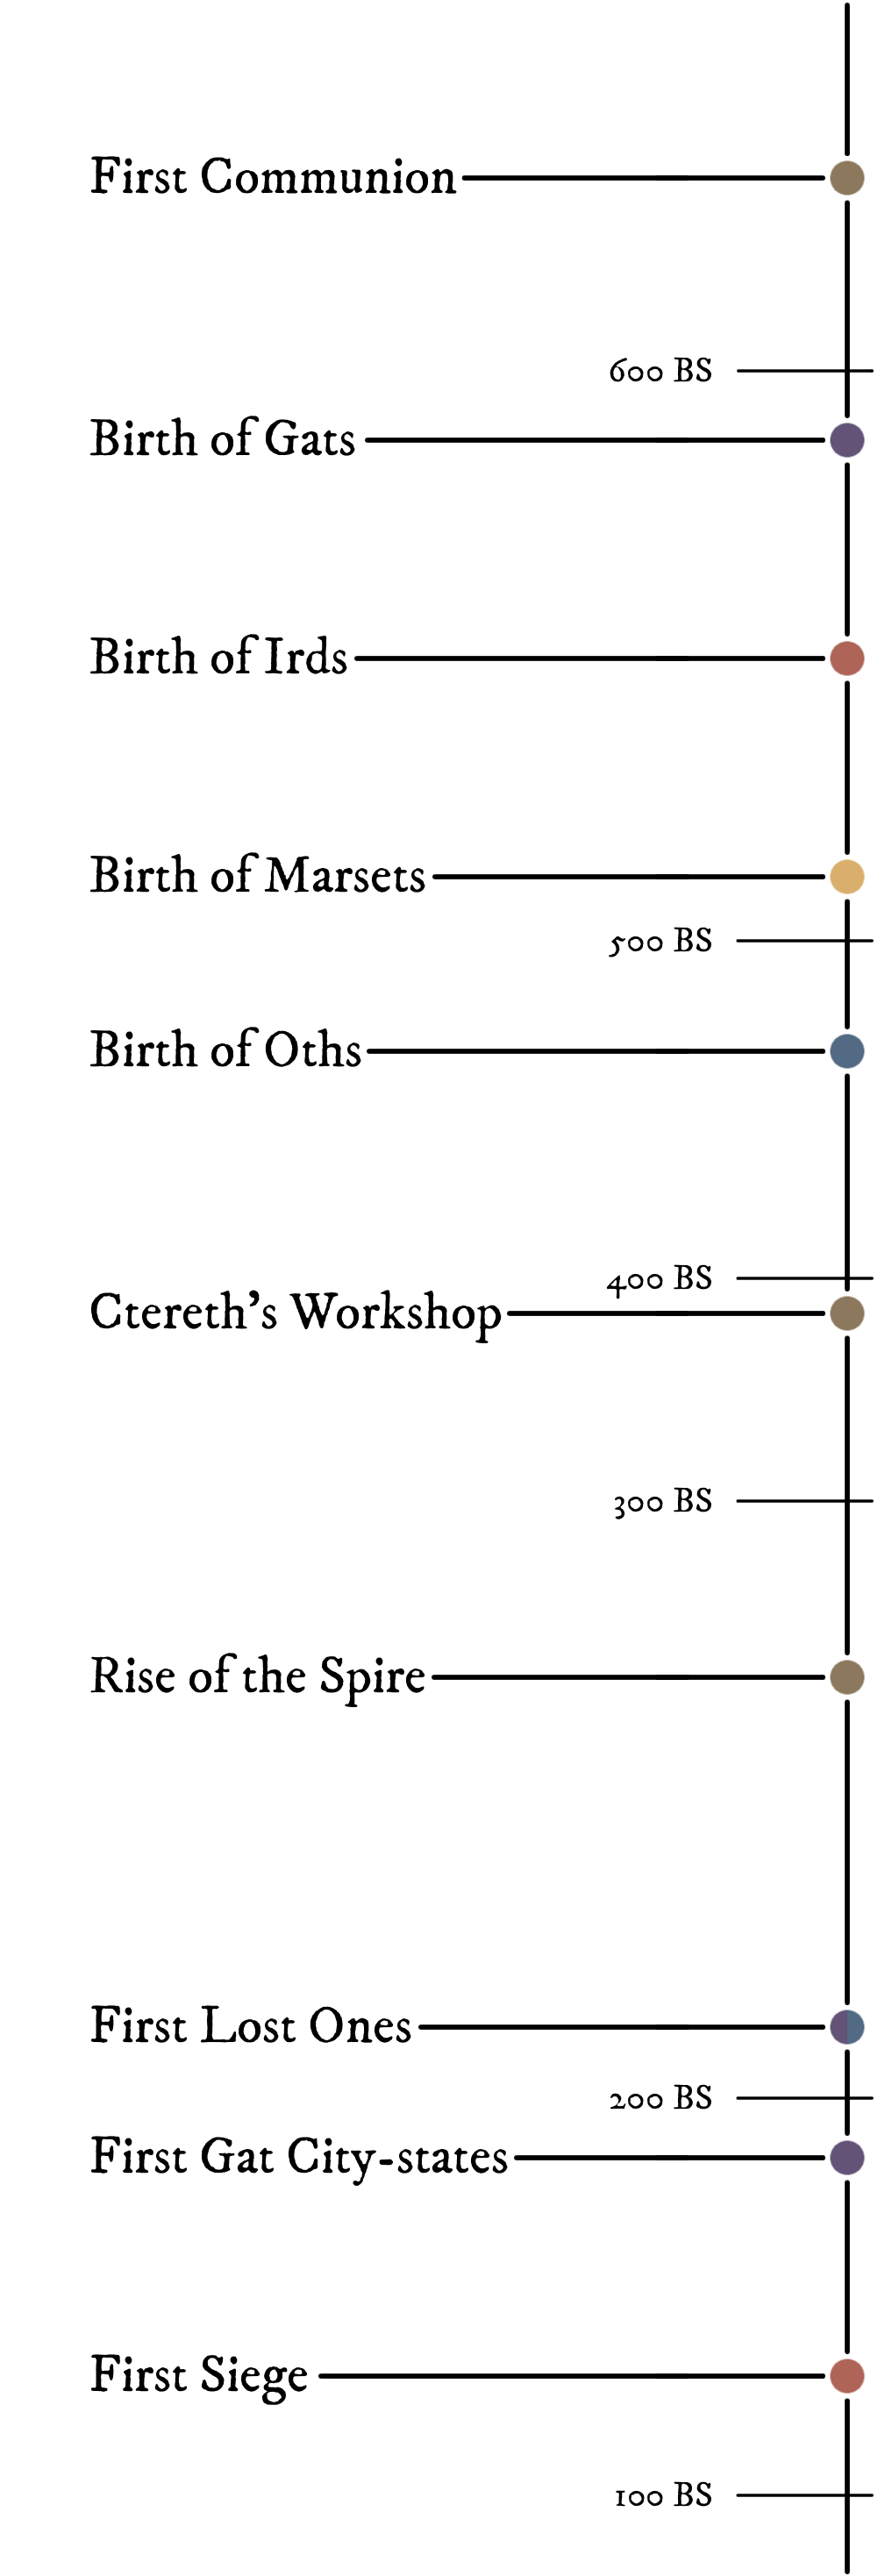
\includegraphics{01yuadrem/img/30history_i.png}
\end{figure}

\section{History} \label{sec::history}
% History is known in detail thanks to the dutiful oths that recorded it under Tol's guidance.
% TODO: Capitalise all the location names, like Arctic Archipelago, Sylvan Canyon, etc.
% TODO: Take a look at the whole cultures and Yuadrem pages and fix years and nation names!

\subsection*{Ancient History}
\subparagraph{682 BS --- First Communion} In the middle of the dead sea, the et E'ukarilth merges with a deceased higher one embryo.
This transforms the tall one into an insane visage of their former self.
The church of E'ukarilth is later founded to attempt communication with the et.

\subparagraph{592 BS --- Birth of Gats} The search for the Lung of Ur begins, an artifact of great value to the tall kin.
The indigo school of the et Thul-yharch creates the hardy gats, believing the relic is below the surface.

\subparagraph{547 BS --- Birth of Irds} With underground search proving unsuccessful, the red school of Zyl'rech births the mobile irds.
Taking to the skies, they survey land and ocean, hoping to find clues of Lung's location.

\subparagraph{523 BS --- Birth of Marsets} The gold school of Tosh-drieln produces the arboreal marsets.
They explore the thick and dark jungles of Yuadrem with ease.

\subparagraph{451 BS --- Birth of Oths} Under mysterious circumstances, oths are created by the et Tol.
Before disappearing, the tall one teaches them writing, and they begin recording history and compiling the findings of the ets and their progeny with great care and detail.

\subparagraph{397 BS --- Ctereth's Workshop} To cope with the uncontrolled population growth of the new kins, the et Ctereth digs a deep cavern in the middle of the dead sea.
Inside it, the tall one builds a workshop and tirelessly crafts qualar to gift the newborns sentience.

\subsection*{Nadir}
\subparagraph{217 BS --- The Rise of the Spire} The tall kin, apparently done with their search, create the spire at the place where E'ukarilth found the higher one.
They build the stone city of Jan'krug atop the mountain.
The progeny kins, now left alone, are forbidden from accessing the dead sea and, incapable of producing qualar, are forced to fight among themselves.

\subparagraph{209 BS --- First Lost Ones} The first plains gats and chu'ash oths are born, separated from their kins by their lack of qualar.
% While ird and marset lost ones also exist, the lack of a qualars doesn't affect these kins as much as their siblings, perhaps due to their wilder nature.

\subparagraph{179 BS --- First Gat City-states} The gats, always fighting adversity, establish the three city-states of Fiele, Avshen, and Alagyaz.
With careful birth control techniques, they manage to maintain a stable population.

\subparagraph{144 BS --- First Siege} A group of three irds known as ``the feathered sunrise'' infiltrates the dead sea and steal tens of thousands of qualar from Ctereth.
The nations of Krudzal, Harual, and Hulnar are later established by their descendants.

\begin{figure}[H]
    \centering 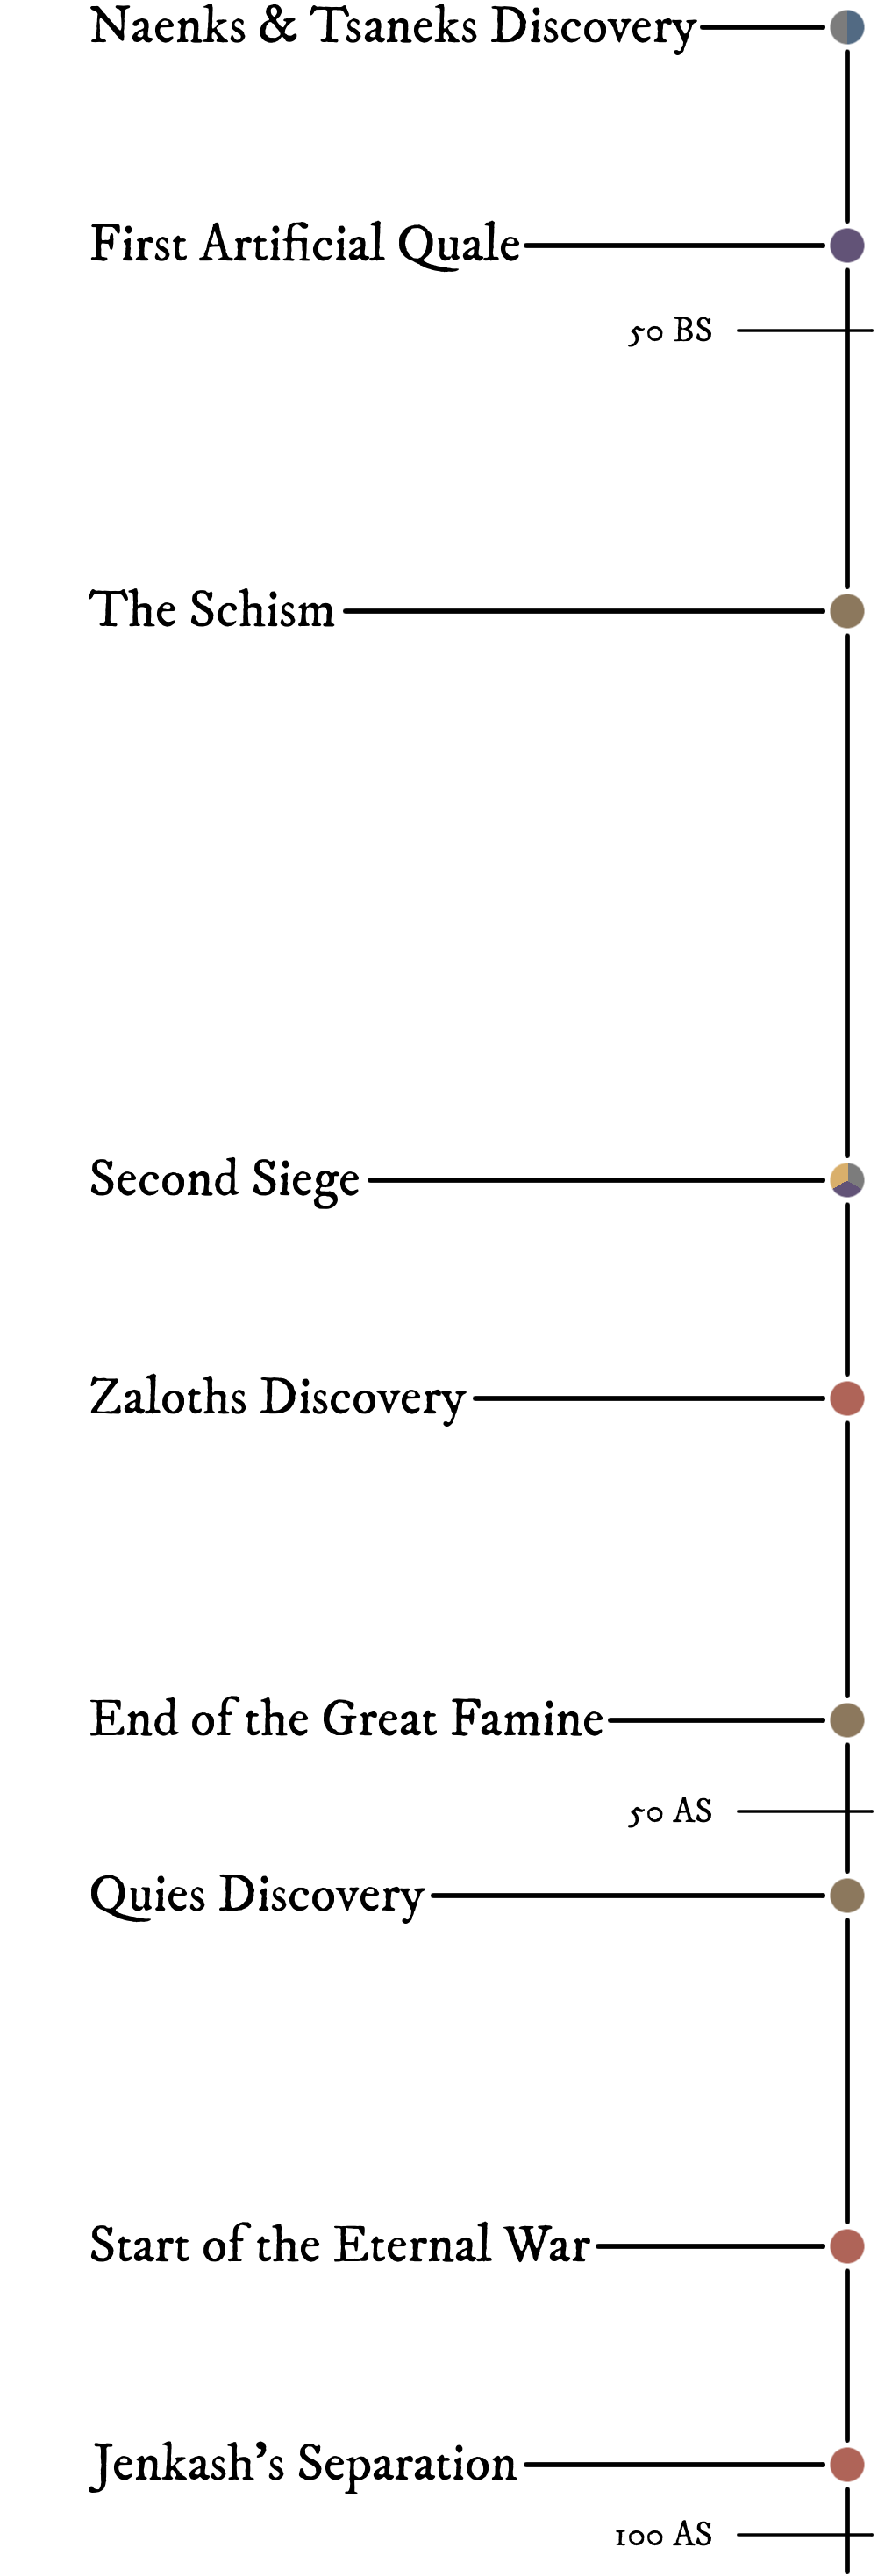
\includegraphics{01yuadrem/img/30history_ii.png}
\end{figure}

\subparagraph{92 BS --- Naenks \& Tsaneks Discovery} Trying to find a home, a group of stray marsets known as the Ovovians, stumble upon the naenks and tsaneks of Drejeck.
These two are inexplicable kins born from mold and fungi respectively.

\subparagraph{51 BS --- First Artificial Qualars} The gat Jirar the bonecarver creates a technique to craft rough qualars imitations.
By passing the practice to the gat's disciples, Jirar unshackles the population number of the kins, and boosts Alagyaz's economy to unprecedented levels.
% To date, only gat master bonecarvers have managed to use the technique. One bonecarver's qualar count usually doesn't go above the thousands, but as populations grow so does the need for qualar.

\subsection*{Great Famine}
\subparagraph{0 --- The Schism} The tall kin's folly causes the schism.
The spire, now revealed to be a dormant volcano, catastrophically erupts.
The event destroys Jan'krug and most of the ets.
The spewed ash blocks off sunlight for four decades, starting the age known as the great famine.

The explosion causes a portal known as the sizzling gate to be opened in a cave inside of the spire.
This door leads to the outer lands, a strange and primal plane that exists outside of Yuadrem.
From the portal spew forth the foreigner kins: the adventurous tortles, the violent grungs, and the ingenious umans, along with the blueblood beasts.

\subparagraph{1 AS --- Second Siege} The foreigner's horde, a great army of tortles, grungs, and umans, siege Ctereth's workshop.
They're successful, and the great number of qualar stolen is used to start their own settlements in Yuadrem.

\subparagraph{4 AS --- Zaloths Discovery} The zaloths, a kin made of fire, ash, thunder, and hail, walk down from the ruins of Jan'krug.
They freely roam Yuadrem, following a nomadic lifestyle that keeps most away from civilized society.

\subsection*{Age of Heroes}
\subparagraph{38 AS --- End of the Great Famine} Satisfied with a death toll in the tens of millions, the ash clouds from the spire disperse, finally ending the great famine.

\subparagraph{57 AS --- Quies Discovery} A group of gat voyagers from Avshen rise up to Jan'krug, finding the city ruined beyond repair, covered by solidified lava.
However, what they do find beneath the ruins are the quies, a new kin.
Quies are the last kin created by the ets, and are brought back to Avshen.
They easily integrate into gat society, despite their physical differences.

\subparagraph{71 AS --- Start of the Eternal War} The newly born kingdom of Krudzal in the north begins a war against the stone giants of the northern territories.
The war rages to this day, with little obtained by the thul'kraka irds.

\subparagraph{99 AS --- Jenkash's Separation} A blossoming nation of qulbaba irds is split into forty-five separate tribes by ideological differences.

\begin{figure}[H]
    \centering 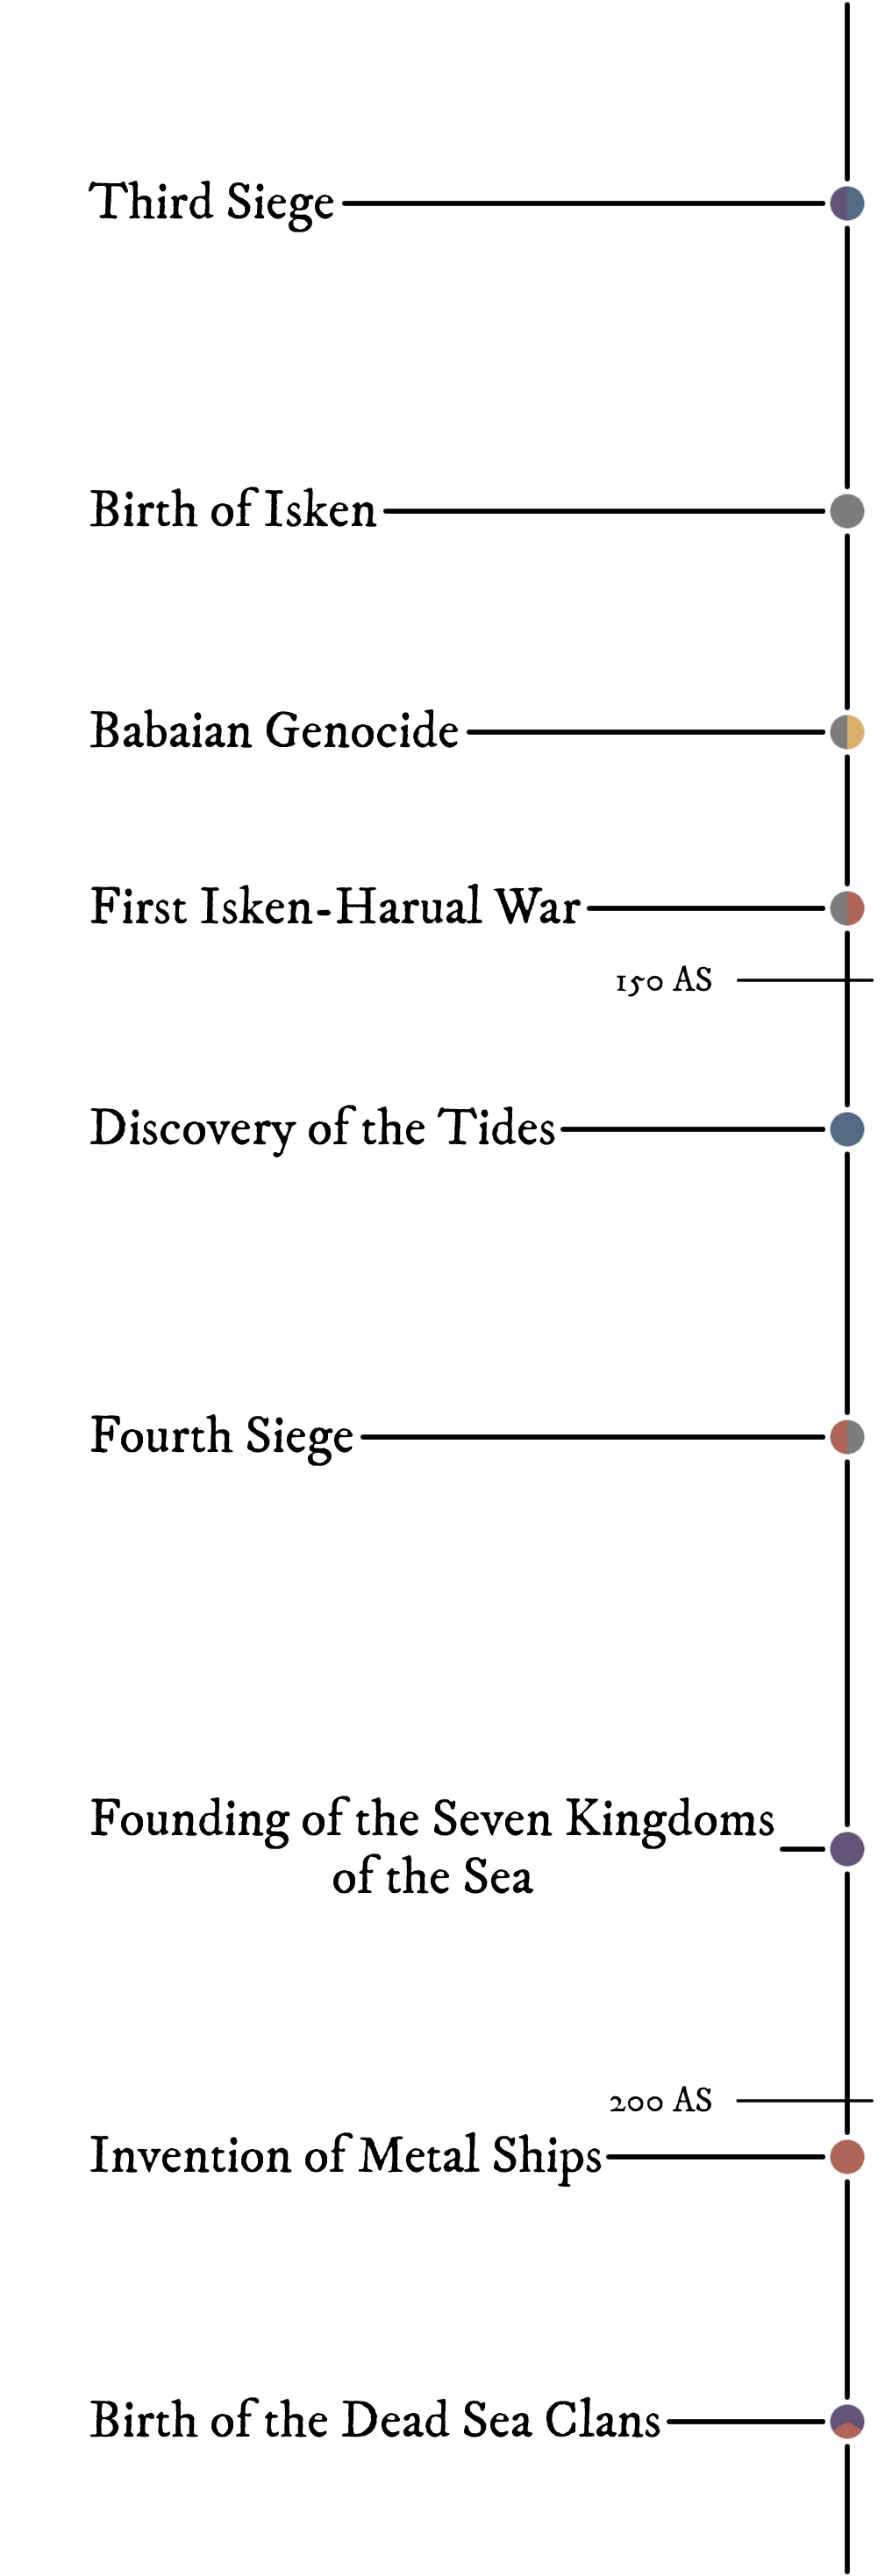
\includegraphics{01yuadrem/img/30history_iii.png}
\end{figure}

The tribes that will eventually become Jenkash are bound to constant conflict, unable to establish a unified government for more than a hundred years.

\subparagraph{102 AS --- Third Siege} Inspired by their siblings lost three centuries ago, the army of healing is formed.
Mainly composed of gats and oths, they successfully invade Ctereth's dwellings, then personally bringing the stolen qualar to the bughna gats and the chu'ash oths, re-integrating them into civilized society.

\subparagraph{141 AS --- Birth of Isken} Among the dark forests of the Chirping Wilds, the grung empire of Isken is formed.
Initially secretive, they will soon become one of the most fearsome forces in Yuadrem.

\subparagraph{143 AS --- Babaian Genocide} The grungs of Isken easily crush the marset nation of Baba, systematically killing the marsets until very few are left.

\subparagraph{144 AS --- First Isken-Harual War} Ever hungry for power and land, the Iskean empire attacks the Harualish tribes of the Chirping Wilds.
This is the start of a long sequence of slow and bloody wars that will last for more than two centuries.

\subparagraph{174 AS --- Discovery of the Tides} The oths from the temple of Ignelli, led by Hashim, unearth the phenomenon of the tides, learning of its influence on the kins of Yuadrem.
The discovery revolutionizes the way the kins perceive their own feelings and motivations, and leads to them questioning the nature of sentience itself.

\subparagraph{189 AS --- Fourth Siege} To cope with their ever-growing populations, a temporary alliance is formed between the dratl ird houses of the west and the grung empire of the east.
Their union leads to the fourth and final successful siege of Ctereth, enabling a great growth for the Hulnar and Iskean empires.

\subsection*{Age of Nations}
\subparagraph{195 AS --- Founding of the Seven Kingdoms of the Sea} Ever-growing in numbers, the gat city-states coasting the whaler's sea coalesce into nations, each under its own king.
With all the events happening in one year, the formation of the seven kingdoms of the sea initiate an age of prosperity for the horned and retainer kins.

\subparagraph{201 AS --- Invention of Metal Ships} Edren, a thul'kraka ird from Krudzal, designs and invents the first ironclad ship.
The design, named after the ird's son, Durkin, boosts Krudzal's trading capabilities and kick-starts a great colonization campaign.

\subparagraph{212 AS --- Birth of the Dead Sea Clans} Imitating their neighbors to the north, many uman, dratl ird, and plains gat clans are established in the dead sea.

% These clans however are very different from the civilized kingdoms of the north.
% Warlords are elected by strength, and their territories are as shifting as the erratic sandstorms.

\begin{figure}[H]
    \centering 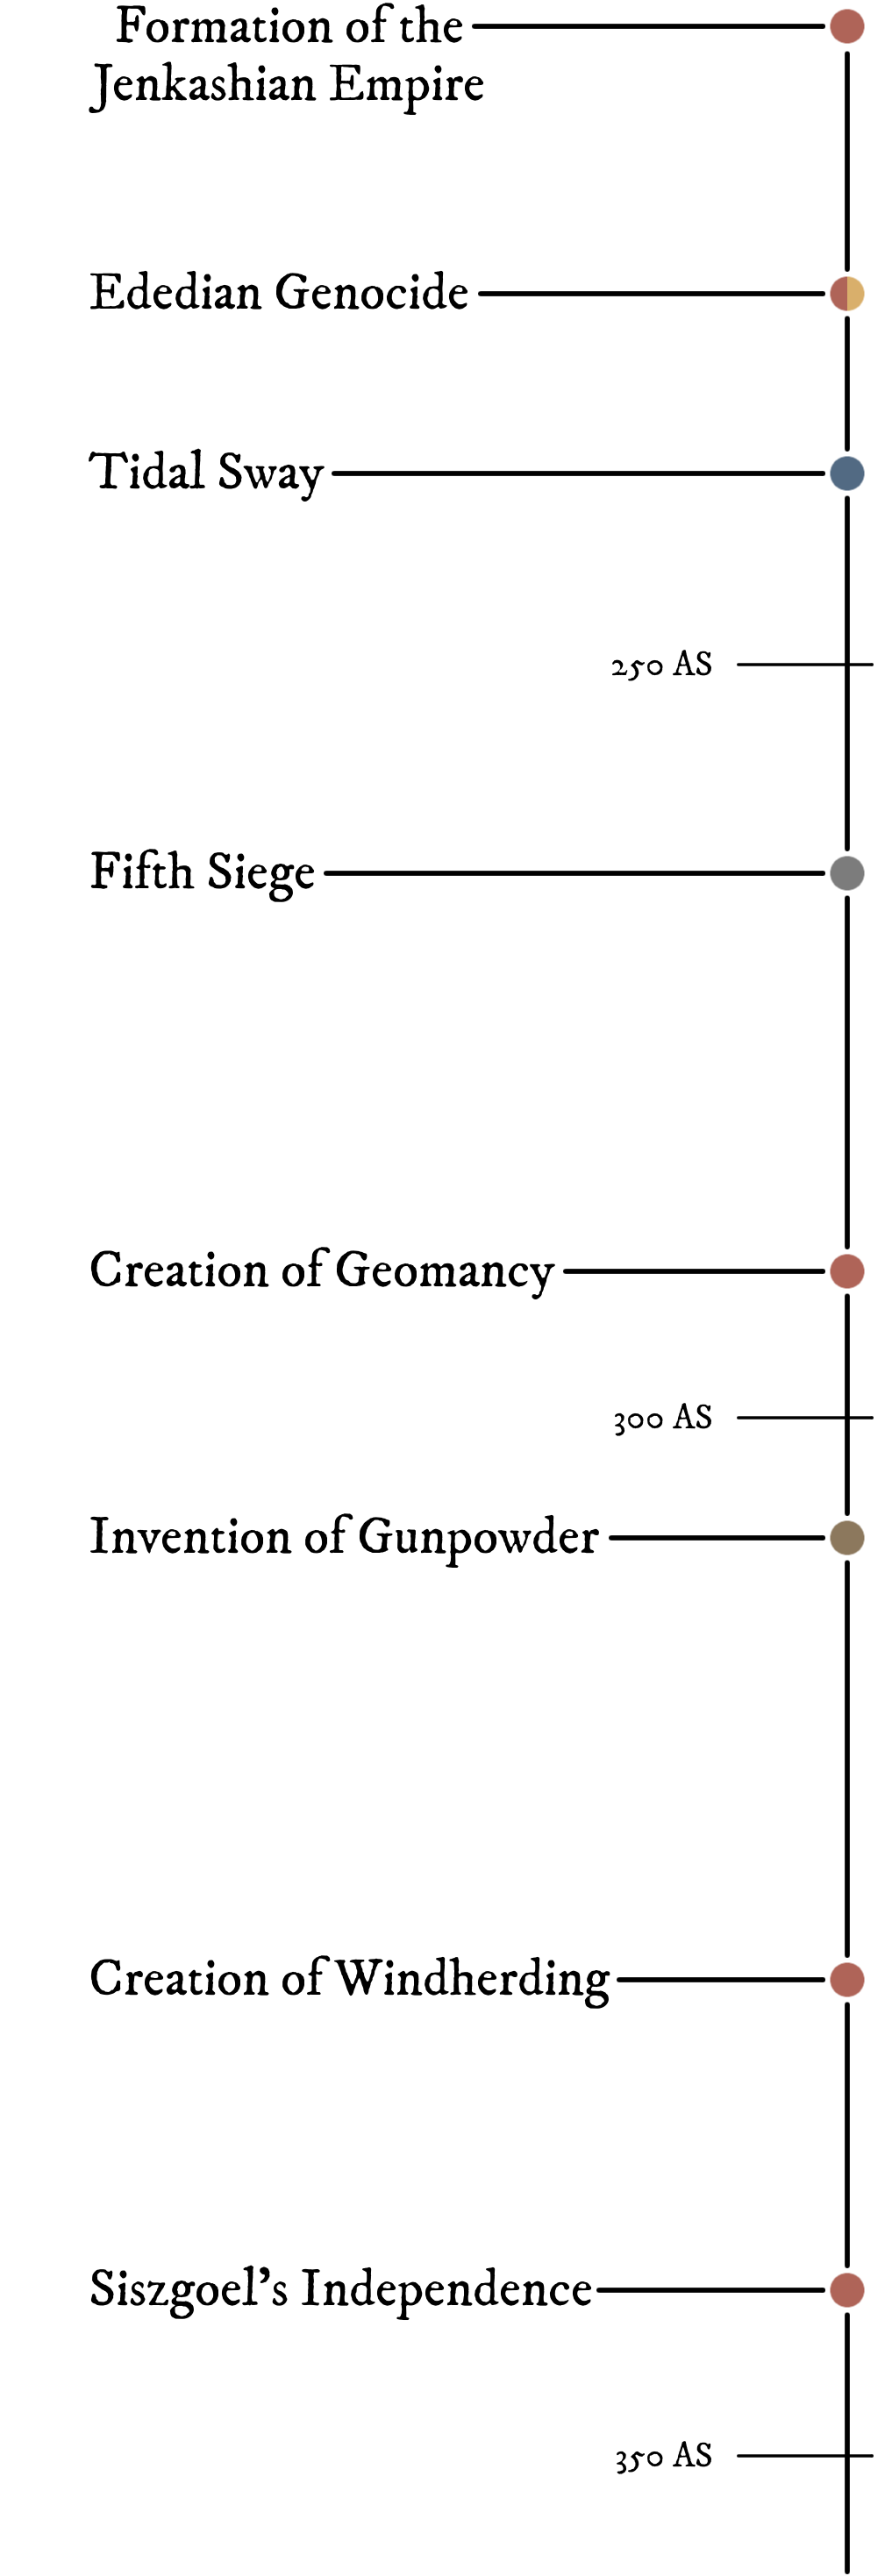
\includegraphics{01yuadrem/img/30history_iv.png}
\end{figure}

\subparagraph{229 AS --- Formation of the Jenkashian Empire} Driven by inner conflict, the irds of the qul archipelago exhaust their natural resources.
This forces them to prematurely end their quarrels, and begin invading and pillaging the surrounding territories.

\subparagraph{231 AS --- Ededian Genocide} The Springwater island is almost completely overtaken by Jenkash, decimating the marset population and forcing most into exile.

\subparagraph{247 AS --- Tidal Sway} Hailing from Ignelli, the oth Narr from the Rashiist school of thought performs an uncanny ritual to harness the power of the tides.
This accidentally triggers the tidal sway.

The oth summons the Sorrow into Yuadrem, ending the life of most Rashiists and ravaging the wildlands entirely, blocking access by land to the southern regions of Yuadrem.

\subparagraph{272 AS --- Fifth Siege} The Iskean grungs, banned from buying artificial qualar from Khedrat, attempt a new siege upon Ctereth's workshop.
This time however they fail, stopped by an unsuspected force: the newly formed dead sea clan of Dzarog.
Dzarog is a clan of umans and gats that live in dens around the spire, and protect Ctereth's caverns for yet unknown reasons.

\subparagraph{281 AS --- Creation of Geomancy} The ird nation of Hairuus, protected from Isken by the splitting mountain range, develop the art of geomancy.
As a test of their mastery of it, they elevate an island at the middle of the shield lake, where their capital, the Nest, is built.

\subparagraph{304 AS --- Invention of Gunpowder} Hailing from the young nation of Sulia, the oth Karmin discovers gunpowder.
With this new firepower, many engineers from Sulia design and build varied weapons, like fire spears, hand-cannons, and muskets.
These new weapons give them a proper combat advantage, allowing them to defend themselves from the savage nomadic tribes of the blank plains, and slowly expand their territories to the east.

\subparagraph{331 AS --- Creation of Windherding} The uncommonly peaceful irds from the Dentrala tribe in Jenkash develop the art of windherding.
The other tribes quickly adapt this art for combat, leading to the Drejeck wars against the naenks of Gannag and the Dratl'fal wars against the declining empire of Hulnar.

\subparagraph{340 AS --- Siszgoel's Independence} Siszgoel, a long-standing colony of Krudzal, declares independence.
The nation of Kaldrathal is born, under the rule of the warrior queen Ialul.
The natural deposits of nitrate in the country's island of residence, Krejek, boosts a powerful gunpowder industry, quickly matching that of Sulia.

\begin{figure}[H]
    \centering 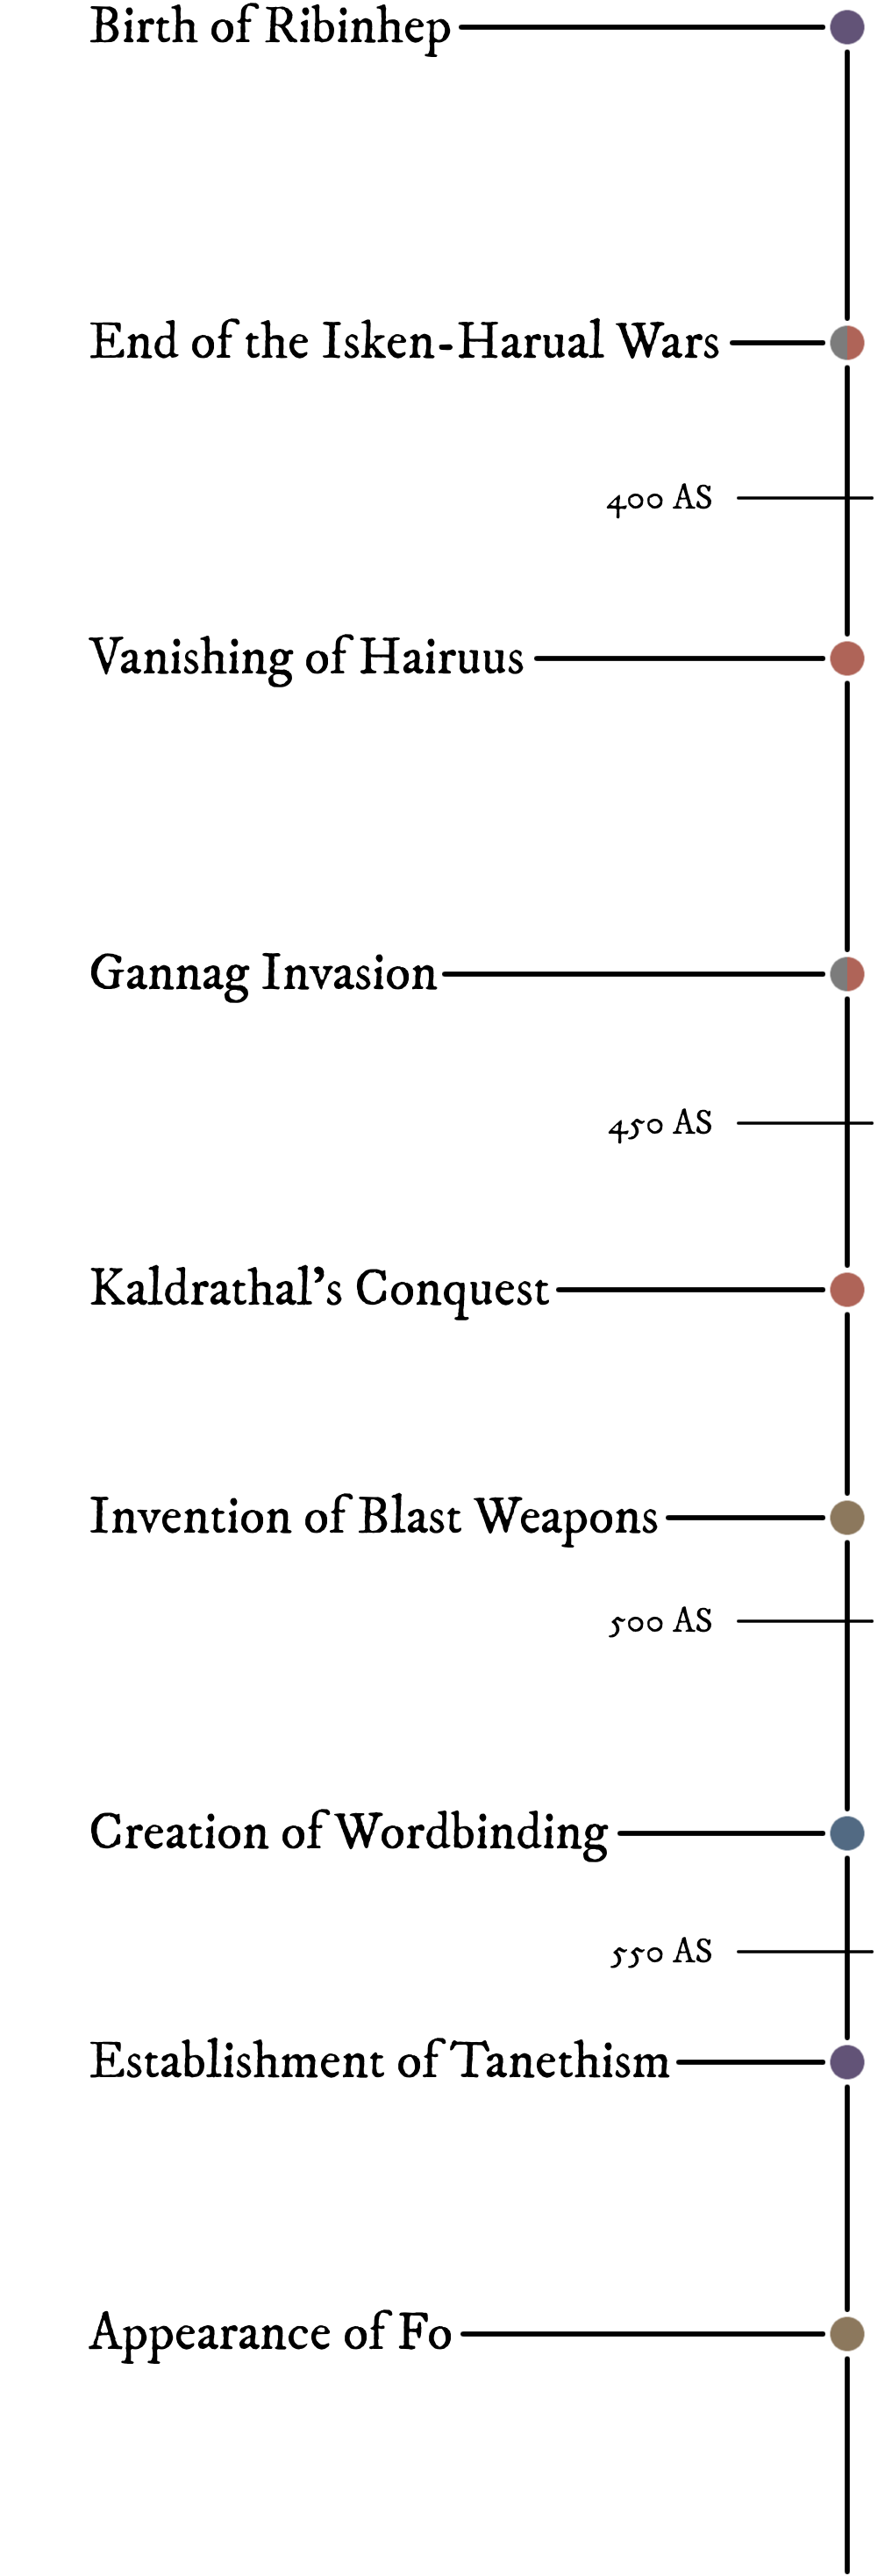
\includegraphics{01yuadrem/img/30history_v.png}
\end{figure}

\subparagraph{354 AS --- Birth of Ribinhep} Umans, a kin commonly hunted an enslaved, manage to establish permanent settlement in the isle of rust.
Naming themselves Ribinhep, they start conquering the northern fjords using their unique mercury weapons, fighting under the rule of the frostburn king Kuin.

\subparagraph{389 AS --- End of the Isken-Harual Wars} After 248 years, the Isken-Harual wars end, with Isken crushing almost all of the ird tribes.
The grung empire quickly proceeds to attack the Byurev nation, attempting to conquer territories up north.
They are however stopped by the gats, prepared for such an invasion decades ago.

\subparagraph{411 AS --- Vanishing of Hairuus} The lake-based country of Hairuus suddenly vanishes, soon after elevating new land for their growing capital.
Rumors that the lake is haunted begin spreading, and nations avoid claiming the empty territories and abandoned cities for fear of this mysterious curse.

\subparagraph{440 AS --- Gannag Invasion} Seeing that the Jenkashian forces are focused on conquering the mainland, the armies of Gannag suddenly invades the qul archipelago under the command of Kutsa the sharp.
In few weeks they manage to conquer half of Jenkash's homeland, taking prisoner irds as sacrifices to use as birth corpses.

\subparagraph{461 AS --- Kaldrathal's Conquest} Most of the islands of the arctic archipelago are claimed by Kaldrathal, who establishes a new form of government that tries to represent the taken territories.

\subparagraph{498 AS --- Invention of Blast Weapons} Reut, an engineer from Drer, invents a new use of Sulia's gunpowder: Blast weapons.
Used for close-quarters combat, blast weapons aim to both surprise and immolate the enemy.
Among the most famous examples are the flame vent, the firecrackers and the flaming pole-arms.

\subparagraph{533 AS --- Creation of Wordbinding} In collaboration, the many oth houses of Palegna create the art of wordbinding.
The technique quickly gains traction, as it adds a method for trustless trade between peoples and nations.

% \subparagraph{553 AS --- Na'ane's Founding} A large circle of tsaneks led by Tsehant, tired of their class-based society, made a pilgrimage to the fog gorge.
% They establish in it, and form the independent nation of Na'ane.

\subparagraph{577 AS --- Establishment of Tanethism} The king of Khedrat, Grigor the Old, establishes the recently born Tanethism as the official religion of the nation.
The other kingdoms of the sea follow soon after, and Tanethism is quickly adopted by most gats.
% Here is when bonereading becomes accepted in the seven kingdoms.

\subparagraph{589 AS --- Appearance of Fo} Strange, twisted creatures start attacking any village coasting the shield lake, causing havoc.
Fo, the kinless inhabitant of the nest is quickly blamed for the creation of this creatures, but all attempts to reach the being have failed.

\begin{figure}[H]
    \centering 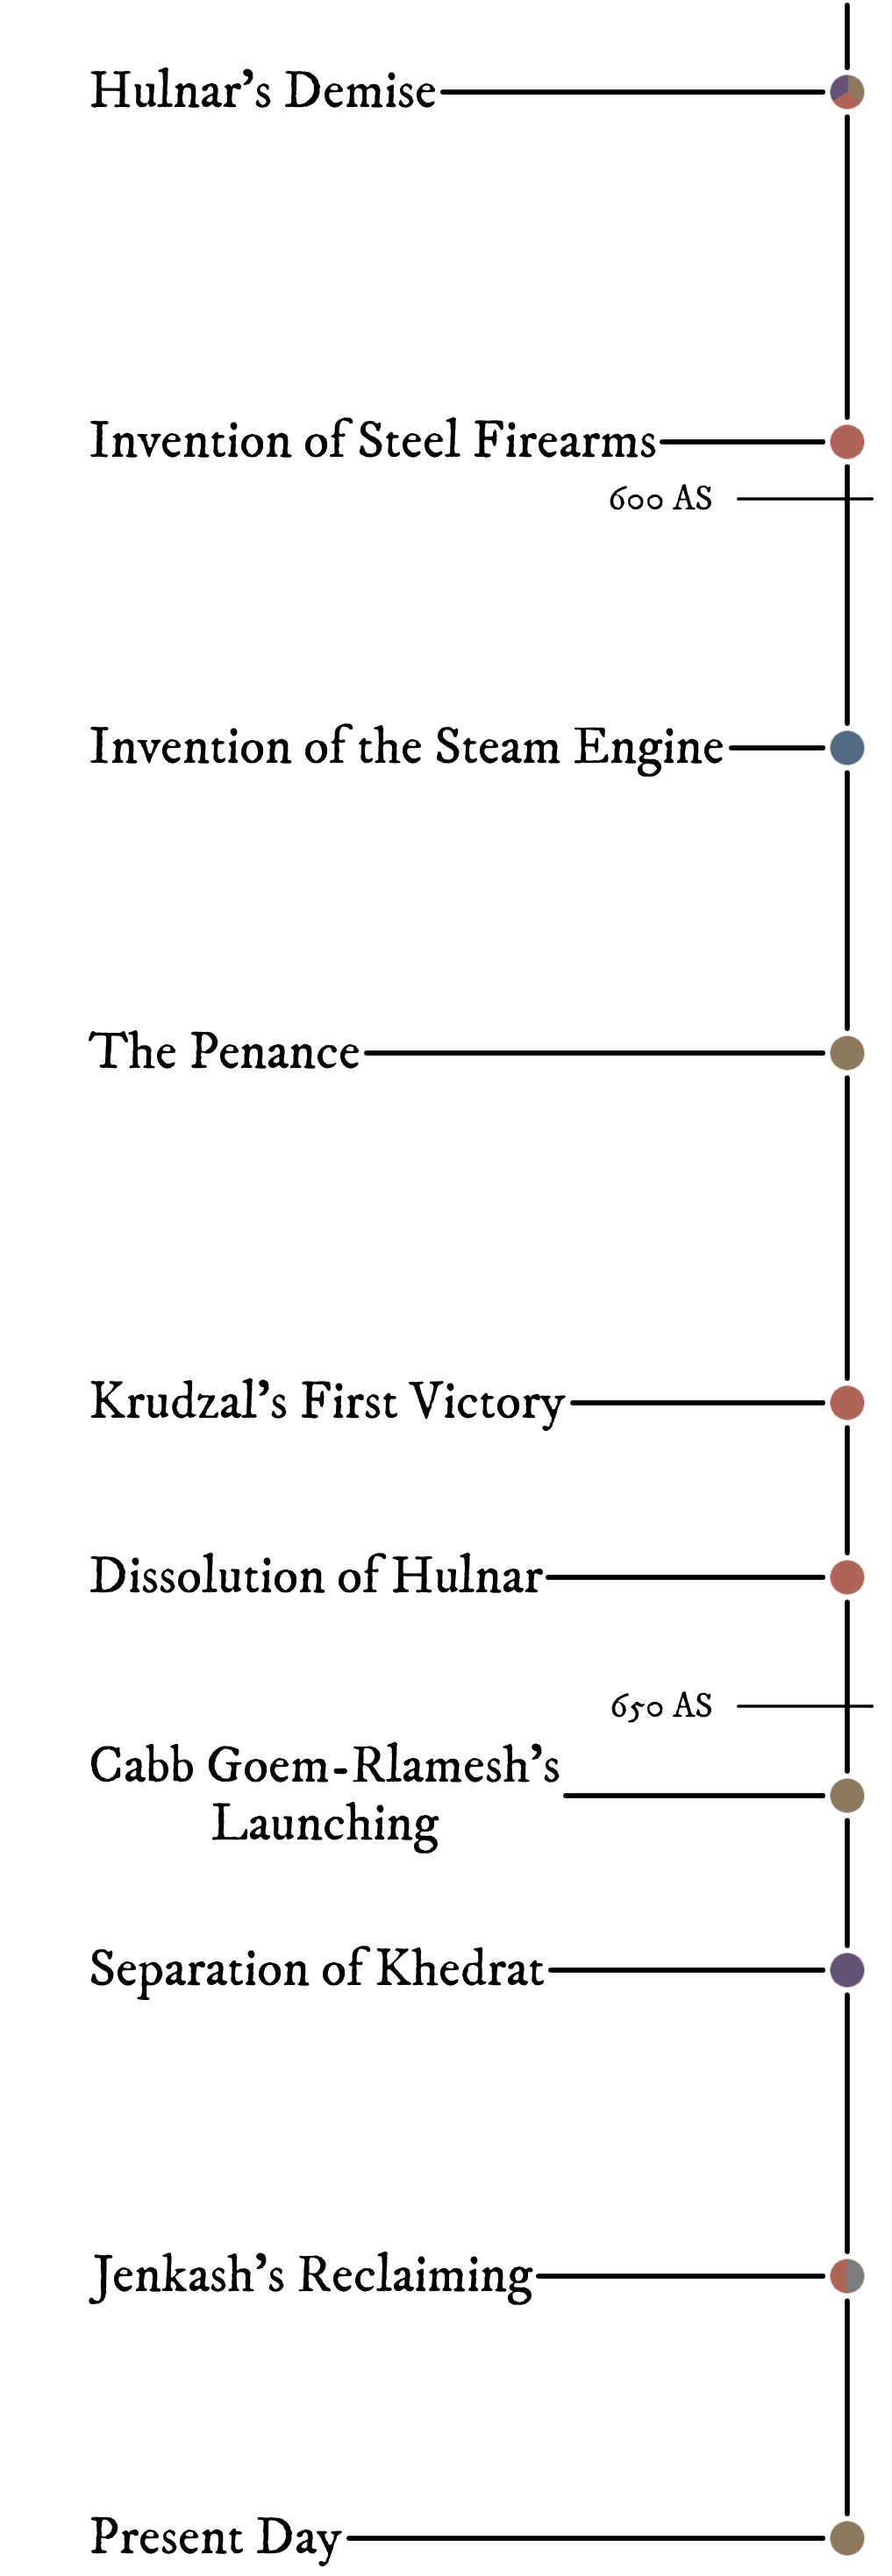
\includegraphics{01yuadrem/img/30history_vi.png}
\end{figure}

\subsection*{Golden Age}
\subparagraph{591 AS --- Hulnar's Demise} The strong alliance between the nations of Khedrat and Sulia defeats Hulnar in the Sylvan wars, allowing both nations to occupy a segment of the Ichor mountains and the entirety of the Sylvan canyon.
This act helps mitigate the pirates' presence in the Whaler's Sea, kick-starting an era of peace and trade for the coastal nations.

\subparagraph{599 AS --- Invention of Steel Firearms} The inventive Kaldrathian engineer Seja combines Krudzal's quench-hardened steel with her new refined gunpowder.
The explosive mix leads to the development of fierce steel-based weapons, including long-range cannons, wheel-lock pistols and sophisticated rifles.

\subparagraph{607 AS --- Invention of the Steam Engine} Away from the economic center of Yuadrem, the Na'anian tsanek Nugut invents the steam engine.
Originally used simply to drain the Na'anian coal mines, the tsaneks were quick to notice its potential and found hundreds of applications for the engine over time.

\subparagraph{621 AS --- The Penance} A surreptitious ritual known only as ``The Penance'' is carried by the citizens of Dzarog.
From the top of the spire, they summon a horrible being known as Cabb Goem-Rlamesh into Yuadrem.
The colossal amalgamate of flesh slowly drags itself towards the east, ferociously protected by the Dzarogian armies.

\subparagraph{628 AS --- Krudzal's First Victory} Using modified Kaldrathal cannons, Krudzal finally manages to kill a stone giant, claiming their first victory in the Eternal War.
% The event strikes fear on the giants, and Krudzal manages to claim their first territories in the mainland.

\subparagraph{635 AS --- Dissolution of Hulnar} Heirless, the king Sul'rech of Hulnar suddenly dies at a young age.
The dwindling kingdom is split into smaller houses, weak ghosts of Hulnar's old glory.

\subparagraph{655 AS --- Cabb Goem-Rlamesh's Launching} The harrowing immensity, Cabb Goem-Rlamesh, reaches the Burnt Ocean and settles some kilometers off the coast of the dry savanna.
% It becomes known as the breathing city.
% All expeditions to the island have ended poorly.

\subparagraph{659 AS --- Separation of Khedrat} The newly-conquered westernmost territories of Khedrat quickly become tired of monarchy, and peacefully claim independence.
Abandoning old traditions, the new countries of Viphogher and Dnomit embrace democracy: a new, king-less form of government.

\subparagraph{671 AS --- Jenkash's Reclaiming} Forced by Gannag to halt their conquest, the Jenkashian empire focused entirely on re-taking the qul archipelago.
Savage battles are fought, and to date they've managed to reclaim most of their lost homeland.

\subparagraph{672 AS --- Present Day}
\newpage

% !TEX root = ../main.tex
% \begin{figure}[H]
%     \centering 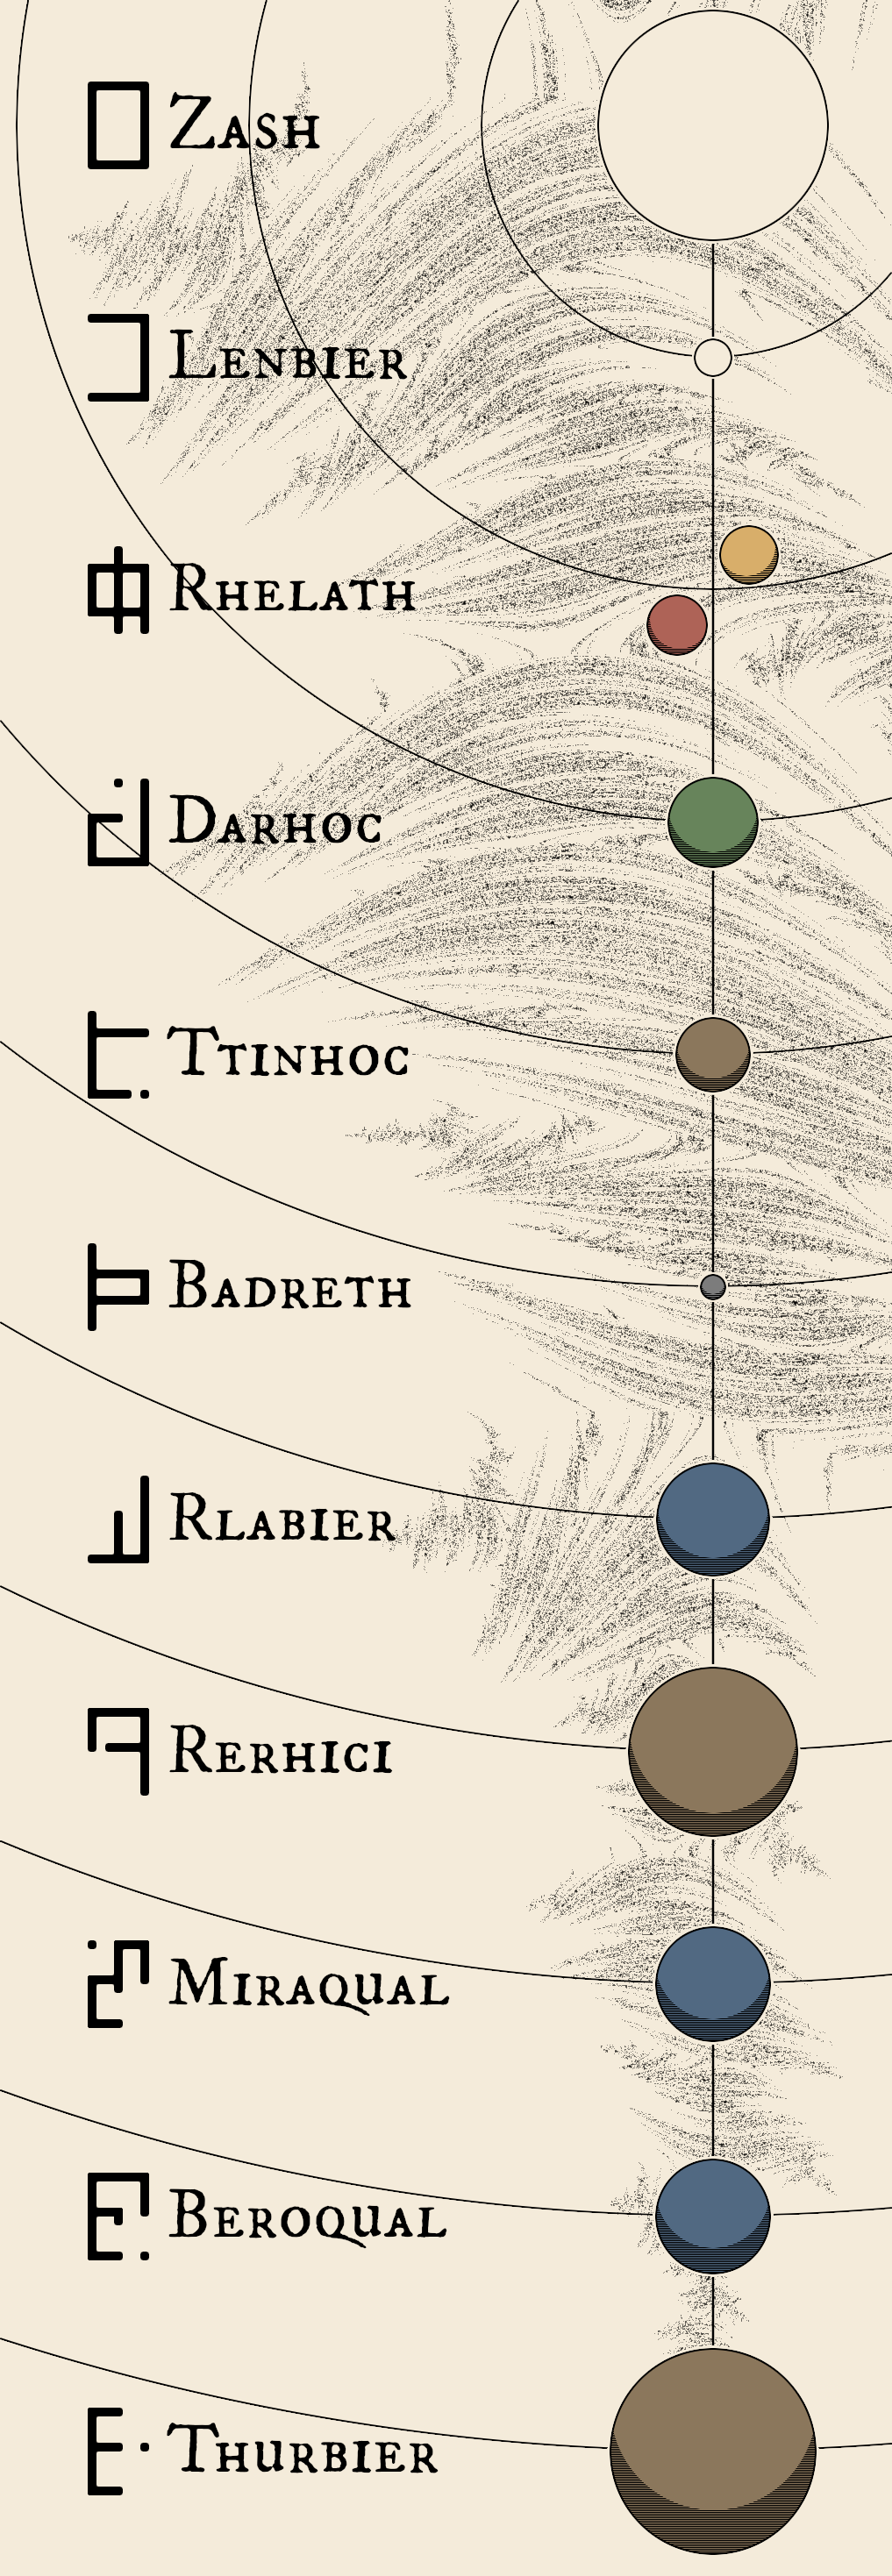
\includegraphics{01yuadrem/img/41solarsystem.png}
% \end{figure}

\section{Outer Planes}
Historically, the perception of the heavens in Yuadrem was inherited from the ets to the original oth scholars.
Despite this early rationalization, most religions still associated the heavens to divine beings or objects of mystical wonder.

% !TEX root = ../main.tex
\subsection*{Cosmology}

\newpage

% !TEX root = ../main.tex
\subsection*{The Five Moons}

\begin{table*}[b]%
    \begin{DndTable}[width=\linewidth]{X}
        \centering
        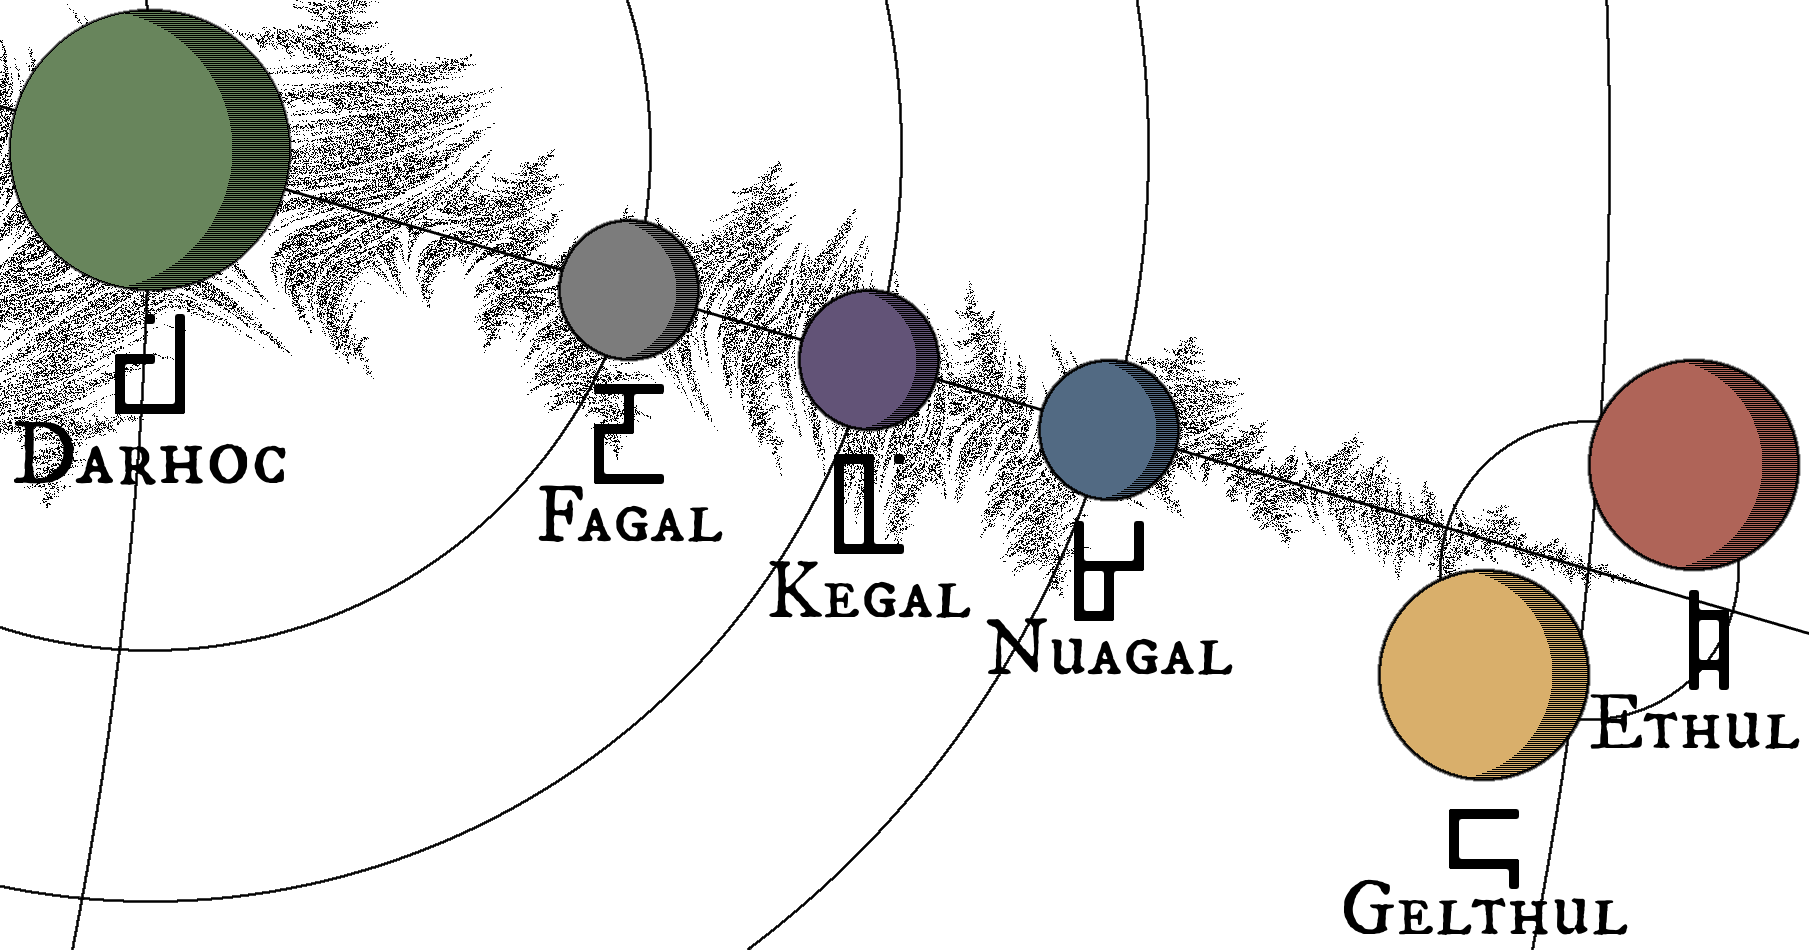
\includegraphics[width=0.99\textwidth]{01yuadrem/img/42moons.png}
    \end{DndTable}
\end{table*}

It is an undeniable fact of nature that moons have a strong effect over the tides.
In Yuadrem, this effect acts both on the ocean's tides and on the inviolate tides of the sentient mind.
Any religion or theory that attempts to explain the tides has to take the moons into consideration, for the two are intrinsecally linked.

The presence of three moons has interesting effects on the ocean tides.
Additionally, the ocassional influence of the twin planets of Rhelath adds more chaos to the system.
For centuries the tides were thought to be unpredictable, as impulsive and erratic as the whims of the mind.

This was until the then unknown oths of Abipolash designed the Nuagalian calendar.
Setting a year to two full translations of Nuagal, it predicts with astonishing accuracy the ocean's tides.
The ability to predict the tides enabled sailors to minimize risk in their journeys.
Some claim that only thanks to this calendar has the Whaler's Sea become the hub of commerce it is today.

There are some who claim to have visited the moons, supposedly through roads paved by the ets of yore.
While there is no substantial evidence to any of these claims, the vivid tales told by these explorers have left many to wonder.

While technically Yuadrem has three moons, the influence of the twin planets of Rhelath over the tides has made history count them as two additional moons.
A list of the moons along with a short description of each is provided.

\pagebreak

\subparagraph{Fagal} The largest and brightest object of the night sky, it is clear that Fagal seeks to be known by all people.
The patron moon of the Silver Tide, Fagal has the strongest influence over Yuadrem's tides, the water rising to kiss its gleaming face.
Its translation period is of 24 days, and its new moon marks the beginning of each month in the Fagalian calendar --- the most common calendar in Yuadrem.

\subparagraph{Kegal} Taking its place behind Fagal, Kegal takes its time to orbit Darhoc, observing even the loneliest commoner.
The patron moon of the Magenta Tide, Kegal's ever watchful eye is always attentive --- and judging --- of mortal lives.
Its translation period is of 48 days, and it is tidally locked to Yuadrem.

\subparagraph{Nuagal} The last of Darhoc's natural moons, Nuagal seems to mind its own business.
Intronspective and absorved, the patron moon of the Blue Tide holds no concern over mortal toil.
Its translation period is of 72 days, rotating freely and independant of Darhoc.

\subparagraph{Rhelath} The patron moons of the Gold and Red Tides respectively, Gelthul and Ethul are two planets locked in an eternal --- and deadly --- dance.
Some say that this dance represents the fiery fight inside oneself, the pull towards helping yourself against helping others.
% Roughly completing an orbit around each other twice a day, each moment that passes these two giants come closer to their eventual crash.

Gelthul and Ethul have orbitted each other for as long as sentience has existed in Yuadrem.%, and all predictions point to this continuing for the countless millenia to come.
The twin planets complete an orbit around Zash every 115 days, and approaches Darhoc every \textbf{TODO} years, wrecking havoc during their visit.

\pagebreak

% !TEX root = ../main.tex
\begin{tikzpicture}[remember picture,overlay]
    \node[anchor=north, yshift=0.10cm] at (current page.north) {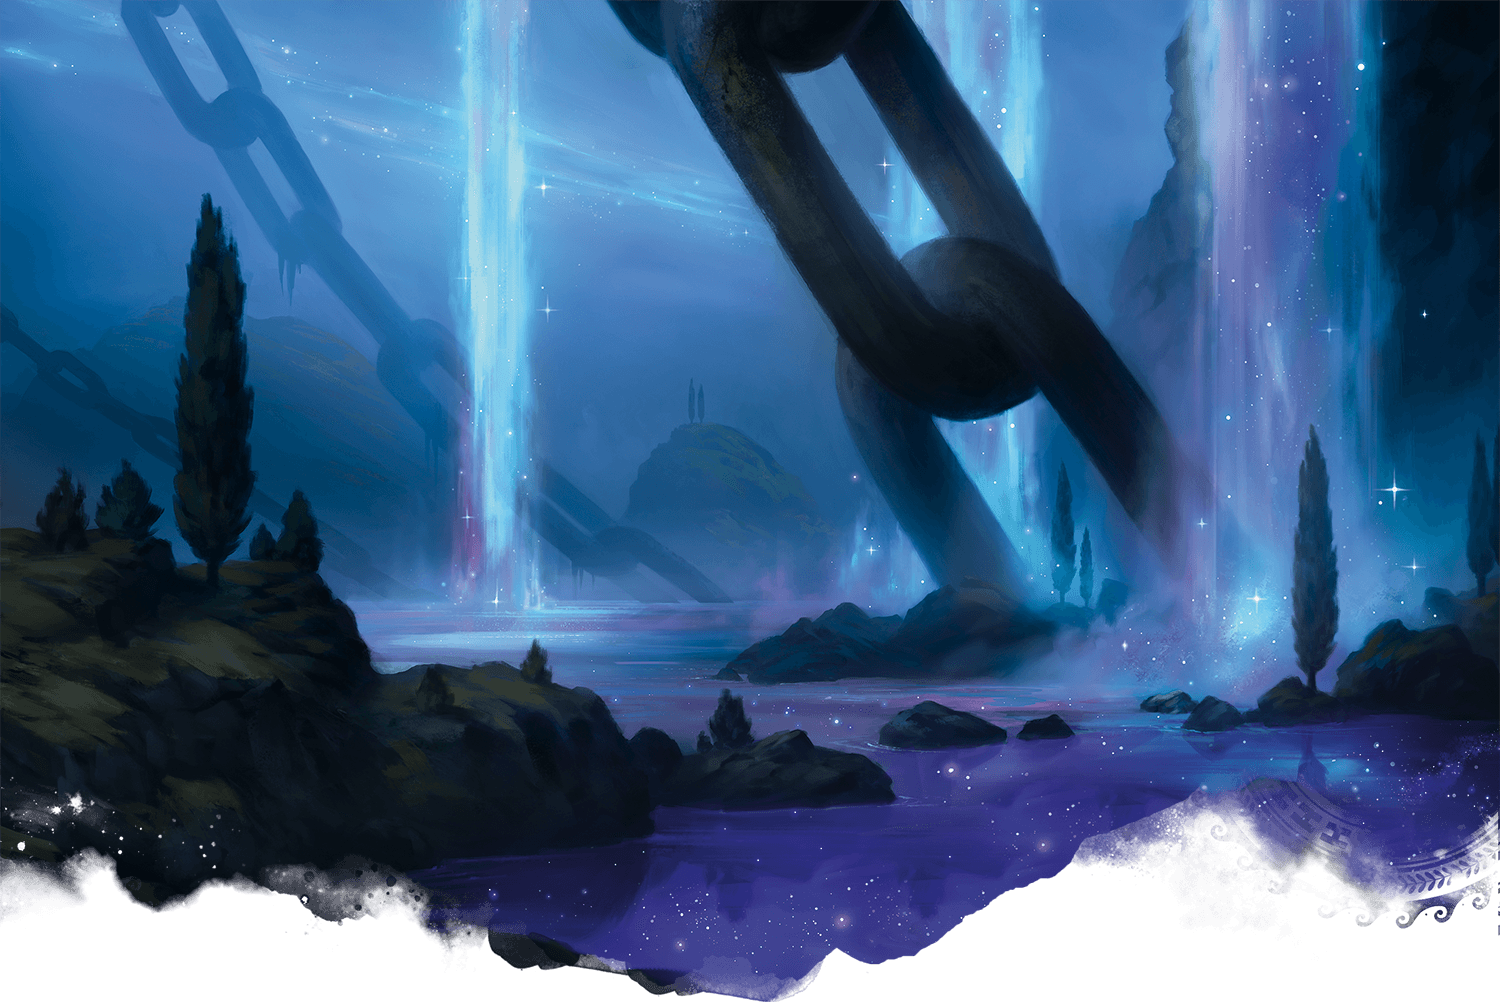
\includegraphics[width=\pdfpagewidth]{01yuadrem/img/43nyx.png}};
\end{tikzpicture}

\vspace{12.0cm}

\subsection*{Nyx}
% \DndDropCapLine{I}{f ever you find yourself beaten and}
% broke.
% And can't feel the wind for the weight of the yoke.
% And fear that the night will not turn into day.
% Remember the darkness will show you the way.
The Schism marked the beginning of an era, and with it came the opening of the Sizzling Gate.
% Through this gate spewed forth the foreigner kins, tortles, grungs, and umans.
On the other side of the portal is a strange realm, thought to be even farther from Darhoc than Thurbier.
Some even claim that this land is not even a planet at all, but an incarnation of the Cosmos itself.
This strange plane is known only as Nyx.

Nyx's topography is similar to that of Yuadrem's, its landscapes characterized by mountains, plains, ridges, etc.
Vast oceans of stars characterize the plane, fed by everflowing waterfalls of nebula.
Thick forests and fields of dark flora cover the shores, grazed by alien creatures known as the Nyxborn.

Titanic ruins and great, algae-slick chains rise out of the sea, as do the weathered remains of forgotten civilizations.
The sky is a misty blur of color that hangs over water as still as glass.
Mighty storms often arise from nowhere, casting souls into waves and whirlpools by the scores.

On especially dark new moons and eclypses, Nyx shows itself in the night sky, its ever-changing brilliance marked by consetellations and cosmic phenomena.
Some claim that during these nights the souls of the recently dead join their anscestors in this strange land.

\pagebreak~
\vspace{13.0cm}

While Nyx is impossible to map, distinct regions do exist, and some travelers have returned to the mortal realm with tales of these incredible locations.
Each of these regions is known as a ward, and is vast beyond understanding.
Most imagine these wards as being stacked atop one another, but their actual relationships defy mortal understanding.

\subsubsection{The Tartyx River}
There is one location however that all who have travelled to Nyx claim to have seen: The Tartyx River.
The Tartyx is vast, with one far shore impossible to see from the other.
Known as the Rivers That Ring the World, it is formed from the confluence of countless tributaries from unnumbered realms.

Countless drifting islands dot the river, some forested by leafless trees, others heaped with crumpling ruins.
Still others are the domains of strange entities that death proves not quite able to claim.
None of these tiny lands are hospitable to either the living or the dead.
The waters of the Tartyx hold their own threats, both mysterious creatures that slither beneath its rippling waters, and their own infamous power to wash away memories and all sense of identity.



    % !TEX root = ../main.tex
\chapter{Mechanic Changes}
\begin{linenumbers}
\DndDropCapLine{S}{trans may break alone, but twisted}
\textit{make a braid. All are not the same, but they shall be as one.
The journey shall be made.}

\hspace*{\fill} --- Anonymous song.

This book includes major mechanical changes.
These mostly focus on allowing players to embrace the worldbuilding aspects of Yuadrem by freeing up their character building options.
These changes are of course optional, but most of the rules in the book were designed with them in mind.

Then, optional rules are included.
Yuadrem is a harsh continent, and these rules help set the atmosphere to reflect this.
They are completely optional, and a healthy gaming table should discuss which should be included or excluded in their game.

\begin{DndComment}{Help Wanted!}
    This entire book was designed with the major mechanical changes considered, yet the author realizes that this can alienate a large part of the community.
    You may want to play in Yuadrem without these changes.
    If this is the case, it is recommended that change many mechanical aspect of the book to acommodate this.

    If for some insane reason you want to take on this challenge, you are encouraged to contact the book's author.
    We could work together on this, discussing appropiate retribution and co-authorship terms.
\end{DndComment}

% \section{Dementia}
% \DndDropCapLine{H}{arsh is the process that awaits the}
% foolish or unlucky enough to lose their qualar.
% Their sentience slips away slowly as they lose their mental capacities.
% Perhaps the worst part is that inward awareness is one of the last attributes lost, forcing them to be fully conscious of the process.
%
% The road towards dementia comes in seven stages, each roughly lasting a week.
% At the moment when you lose your qualar, you enter the first stage of dementia.
% After a week, you roll a DC 15 Intelligence saving throw.
% On a fail, you enter the next stage of dementia.
% On a success, you stay on your current stage and roll again at the start of the next week.
% Dementia is unavoidable, and the DC increases by 1 after every successful roll.
%
% \subsubsection{First Stage}
% No obvious signs of dementia, only minor short-memory loss occurs.
% The main symptoms are associated to the anxiety from the loss of the qualar.
% You start focusing more on your past, often drifting away into daydreams.
%
% You suffer the following effects:
% \subparagraph{Decreased Awareness} You roll for initiative and Dexterity saving throws with disadvantage.
% \subparagraph{Restlessness} Roll an DC 12 intelligence saving throw right after a short rest.
% On a success, you recover your hit points normally.
% On a failure, you only recover half of the hit dice rolled (rounded down).
%
% \subsubsection{Second Stage}
% The self realization and awareness that something is wrong settles in.
% You refuse to accept that your mind is slipping away.
% The more effort you put on remembering the more deterioration your memory suffers.
% Confusion starts setting in.
%
% In addition to the effects of the first stage, you suffer the following effects:
% \subparagraph{Lack of Recollection} Any ability check made to remember or recollect a memory is done with disadvantage.
% All Intelligence (History) checks are made with disadvantage.
% \subparagraph{Mood Swings} All Charisma ability checks and saving throws are made with disadvantage.
%
% \subsubsection{Third Stage}
% You experience increased forgetfulness and might find concentrating difficult.
% You are presented with some of the last coherent memories before confusion fully rolls in.
% Some singular memories become more disturbed, isolated, broken, and distant.
% These are the last embers of awareness.
%
% In addition to the effects of the last stages, you suffer the following effects:
% \subparagraph{Decreased Concentration} All Constitution saving throws made to maintain concentration are made with disadvantage.
% \subparagraph{Vagrant Mind} Intelligence and Wisdom ability checks and saving throws are rolled with disadvantage.
%
% \subsubsection{Fourth Stage}
% Grey mists form and fade away in your memory.
% The ability to recall singular memories gives way to confusion and horror.
% You struggle with daily tasks, presenting clear cognitive problems.
%
% In addition to the effects of the last stages, you suffer the following effects:
% \subparagraph{Motor Difficulties} Strength and Dexterity ability checks and saving throws are rolled with disadvantage.
% Attack rolls are made with disadvantage.
% \subparagraph{Drifting Conscience} In combat, roll a DC 8 Intelligence saving throw at the start of every turn.
% On a failure, you forget where you are, and cannot take any actions during the turn.
%
% \subsubsection{Fifth Stage}
% You have major memory deficiencies.
% The few lapses of consciousness you get are filled with dread, as you realize your mind has mostly left you.
% The repetition and rupture gives way to calmer moments, as the unfamiliar becomes familiar.
%
% In addition to the effects of the last stages, you suffer the following effects:
% \subparagraph{Loss of Fortitude} All rolls are made with disadvantage.
% \subparagraph{Complete Unawareness} All Intelligence (Investigation), Wisdom (Insight), and Wisdom (Perception) automatically fail.
% Your passive investigation, insight, and perception become 0.
%
% \subsubsection{Sixth Stage}
% Your mental state is beyond description.
% You struggle to remember your early life, even forgetting the names of your family and fellows.
% Your capacity of speech is severely impaired, and you suffer sudden and radical personality and emotional changes.
%
% In addition to the effects of the last stages, you suffer the following effects:
% \subparagraph{Declining Speech} You automatically fail all Charisma ability checks and saving throws, and have a very hard time communicating verbally.
% \subparagraph{Hope Lost} As your conscious mind fights your natural tendencies, you automatically fail death saving throws.
%
% \subsubsection{Final Stage}
% Everywhere, an empty bliss.
%
% You make what will most likely be your last die roll, this time with no disadvantage.
% Roll a d20 on the post-dementia table.
% You suffer the effect rolled.
%
% \begin{DndTable}[width=\linewidth, header=Post-dementia Effects]{lX}
%     \textbf{Roll} & \textbf{Effect} \\
%     1 & Your last emotion is rage. You become mindless and violent, attacking your companions without reason. \\
%     2-5 & Your last emotion is apathy. You endlessly stare at the east until you die of natural causes. \\
%     6-18 & Even after brain death, you seek survival. You wander off, attacking any who try to stop you. You become a lost one. \\
%     19 & With memories gone, your mind is fully pulled by its tidal impulses. You lose control of your character, who becomes a servant of The Sorrow. \\
%     20 & Go back to the first stage of dementia, and gain a rank in the Dementia Insight heroic talent.
% \end{DndTable}
%
% The only conventional way to remove dementia is to obtain a qualar again.
% When this happens, you go back one stage of dementia per day passed.
% While in this state you suffer a terrible fever.
% At the beginning of each day roll a Constitution saving throw.
% On a failure, you gain one level of exhaustion.
%
% \section{Hardcore Rules}
% \subsection*{Critical Hits}
%
% \subsection*{Encumbrance}
%
% \subsection*{Hunger and Thirst}
%
% \subsection*{Minor and Major Injuries}
%
% \subsection*{Only One Chance}
% As a rule, you only have one chance to succeed in any action.
% Once you have rolled the dice, you many not roll again to achieve the same goal.
% You need to try something different or wait until the circumstances have changed in a substantial way.
% Or let another PC try.
%
% This rule does not apply to combat, where you can attack the same enemy until it becomes a bloody pulp.
%
% \subsubsection*{Opportunity Attacks}
% In a fight, everyone is constantly watching for enemies to drop their guard.
% While heedless movement is easily punished, any lack of concentration or unplanned action can have devastating consequences.
% Various actions provoke opportunity attacks from a creature:
% \begin{itemize}
%     \item Moving out of the creature's reach.
%     This doesn't apply when someone or something moves you without using your movement, action, or reaction.
%     \item Picking up an item from the floor while in the creature's reach.
%     \item Unsheathing a weapon while in the creature's reach.
%     \item Donning or doffing a shield while in the creature's reach.
%     \item Using the Attack action with a ranged weapon in a creature's reach.
% \end{itemize}
% You can avoid opportunity attacks during your turn by taking the Disengage action.
%
% \subsection*{Short and Long Rests}
%
% \subsection*{Stamina}

\end{linenumbers}

    \DndSetThemeColor[DmgCoral]
    % !TEX root = ../main.tex
\chapter{Kins}
\begin{linenumbers}
\DndDropCapLine{C}{ountless millenia before any of the}
modern kins were born, the ets were born into the land of Yuadrem.
% They were named by the other kins, their creations, due to their impressive size.
They were commonly known as the tall kin, for they usually stood well beyond 3 meters.
Their skin was of a pallid, almost bluish white color, and their eyes were as black as the abyss.
% Most ets didn't have any hair.

The species greatly developed their technology, which was biological in nature.
Free from aging and illness, they developed astonishing physical capabilities despite their apparent frailty.
Each et was indeed capable of shaping their own flesh, causing a great variety of characteristics in the many members of the kin.

Ets were obsessed with their individuality, and it was common for them to change their own appearance, molding their flesh to reflect their personality and philosophy.
Despite their longevity however, it was rare for new ets to be born, and the kin never grew to more than a few thousand members.

\subsubsection{Schools of Thought}
Their longing for longevity led them to study the cosmos, trying to find meaning in the stars.
These studies manifested in the form of the schools of thought, large organizations representing different ways of thinking about the cosmos and oneself.
These schools were their main form of government.%, where individuals were represented by their schools.

Among these organizations, the church of E'ukarilth was of special significance.
More than a thousand years ago, an event known as the first communion took place.
During a pilgrimage to the dead sea, the et E'ukarilth found the deceased embryo of a species yet unknown to its kin, which the tall one dubbed ``the higher kin''.

In an attempt to understand this newfound race, the tall one fused their body with that of the higher one.
The ritual was successful, but it transformed E'ukarilth to an insane, shapeless blob.
Later, the church of E'ukarilth was born to attempt communication with the mad et.

As the gospel of E'ukarilth spread, the kin became convinced that they were utterly insignificant to the cosmos.
The fear caused by this thought elevated their pursuit of individuality.
They believed that the higher kin held a method to become significant, and their schools of thought shifted their studies to focus solely on this strange species.
They believed that with this study they would attain something they called ``the rapture'', described as an ascension to a higher plane of existence.

Their unwavering pursuance eventually led to the schism.
The schism is the most devastating event in Yuadrem's history, causing a 40 year long famine and scarring the land itself for the centuries to come.

\subsubsection{Language}
The tall kin spoke a very sophisticated language, known as jan-theth rlin, simplified as jantherlin.
This language allowed for a very profound expression of one's emotions and inner state, and is still used in poetry to this date.
For when deeper communication is needed, ets could meld their bodies and share thought, but the practice was only used in special rituals or to express especially complex abstract concepts.

As for written word, it was customary for the tall kin to chisel the stone, commonly carving a great variety of images alongside the text.
While this written language originates from jantherlin, each tall one had its own personal version of it.
Other ets could only comprehend one's writing as much as they understood the writer.
This makes the study of jantherlin extremely difficult to modern archaeologists.
% This makes the reading of the jantherlin extremely difficult for the kin that remain in the world, since understanding a particular tall one's scribbles essentially requires understanding their own version of the language.

\begin{figure}[t]
    \centering
    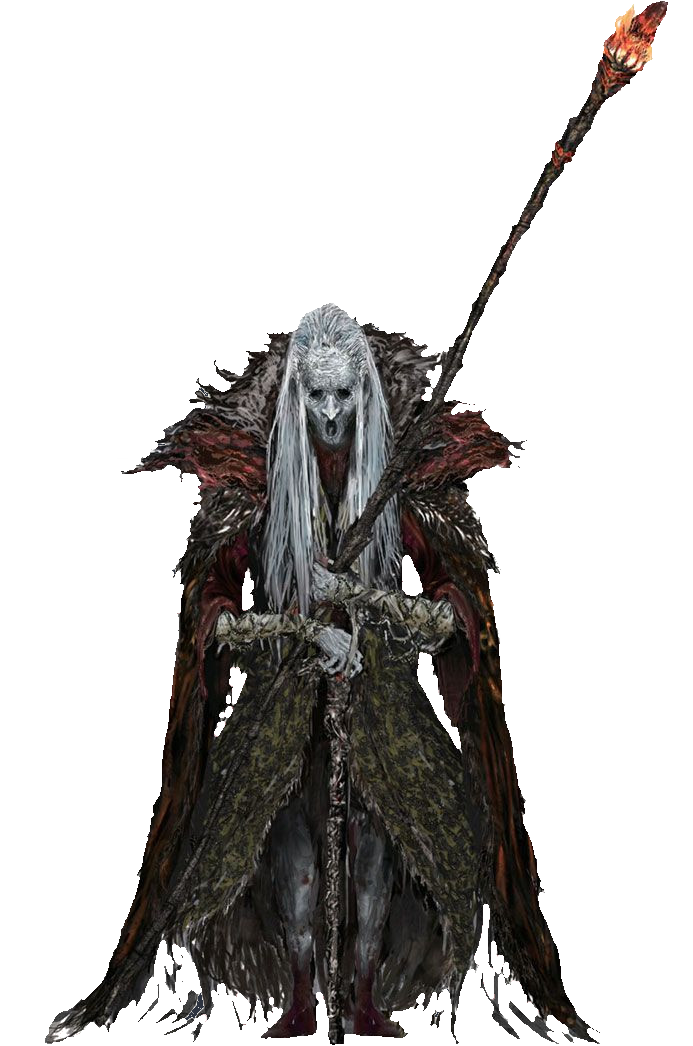
\includegraphics[width=0.45\textwidth]{03kins/img/10et_cleric.png}
\end{figure}

% \subsubsection{Relationships}
% Either by accident or by conscious decision, the tall kin created many of the modern peoples in experiments and studies.
% Most of these held a very high regard for the ets, with some even building entire churches to them.
% However, after it was learned that the they were responsible for the schism, all churches were forcibly shut down, and any adoration is severely punished.
\end{linenumbers}

% !TEX root = ../main.tex
\begin{linenumbers}

\section{Horned Kin}
\DndDropCapLine{W}{hen you contract a horned one, be}
\textit{sure to pay them double.
Fulfill all their needs as they seclude into their workshop, and pay no mind to their uncanny silence.
Most of all, be sure to avoid interrupting them.
Just wait.
The prize that will arrive after they're done working is sure to outshine all your other possessions, and hold a special place in your collection for you and your descendants.}

\hspace*{\fill} --- Orr, Vesjen's master smith.

Citadels carved into the highest of cliff faces.
Mines hidden inside the deepest of ravines.
Workshops rumbling with the sound of hard labor until the darkest of hours.
These are the traits that define the gat.

The gat, marheth'llal rlue, or horned kin are the oldest among the sentient races created by the ets.
Molded as diggers and laborers, their passion for work is ingrained into their very blood.
To date they are known as master miners, builders, and artisans.

Being the first of the kins, they are established and well-developed.
Gats are the builders of the Seven Kingdoms of the Coast, the oldest active nations in Yuadrem.

\subsection*{Beard and Horns}
The horned kin was designed in the image of goats, and share their horns, facial features, and digitigrade feet.
They stand in a hunched manner and are generally slender.
Gats are covered by a thick layer of fur ranging in hues from light blonde to absolute black.
Many enjoy growing a beard.

Gats' eyes are of strong colors, usually light blue, yellow, orange, or light brown.
Like goats, their pupils are rectangular and elongated.
The manner in which each gat's beard and horns grow is unique, and most take pride in these features, showing them off whenever possible.

Gats are genderless creatures.
All gats are born with a pair of seeds hidden in a small sack between their legs.
Around the age of 30, a gat reaches physical maturity.
This is signalled by a slight swelling in these seeds, which they can now cut and plant under a thick layer of rich soil.

While underground, the seed will grow by leeching nutrients off the earth.
After a gestation period of around 2 years, the gat will dig their way up from the ground and emerge as a somewhat competent infant.
A gat would-be-parent must always be careful about where to plant their seed, for if a newborn sees the sun or any strong light during their first days, they run the risk of being permanently blinded.

\subsection*{Adaptable and Hardy}
Gat share many traits with the common goat.
They dwell on bleak mountaintops, deep ravines, rocky hills, and open plains.
While adult gats are not sensitive to sunlight, most prefer dark places.
These predilections lead to gat towns and cities being built underground or in harsh cliff faces.

Never satisfied with their homes, the horned kin's hubris leads to their cities to reach depth and size.
Raids against smaller gat city-state are common, and the gats take them as a chance to test their impenetrable defenses, complex traps, and combat-hardened military skills.

\subsection*{Peaceful Demeanor}
The horned kin are peaceful creatures and mostly shun external conflict.
They are very sociable creatures, and all city-states have one large marketplace in their center for merchants and caravans to settle in.
Surrounded by inns and taverns, these markets act as the commerce hubs of the city.

Community lifestyle is very important to gats, and most wouldn't flinch to give their lives for their city-state.
Due to the gats' slow reproductive cycle, their cities are very welcoming to other species.
It's common to find cities and towns where less than half of the total population is gat.
They treat other species as kin, but high political and military ranks are exclusive to gats.

\subsection*{Impulse towards Greatness}
It is rare for a gat to willingly leave their home, and most spend their entire lives in one city-state.
However, some do feel the call to adventure, and most follow it to gather rare crafting materials or to fulfill a task needed by their community.

Gats are meticulous individuals, and this naturally extends to adventurers.
They won't step into the wilderness unprepared, sparing no expense in armor, weapons, utilities, and the training to use all of this.

Gats are naturally family-oriented, and its very rare for one gat to abandon their progeny.
In the rare occasion that a gat does decide to leave their community behind, it is written law to leave one child or seed planted back home.

This tradition serves a double purpose.
First, the child acts as a magnet to their parent.
Second, in the event that the child is orphaned, their mere presence at least maintains a steady population number.
These gats are the ``Children of the Collective'', and it is tradition that they are taken care of by the whole city, thus nurturing a strong sense of community.

\subsection*{Gat Names}
All gat tongues are simple and practical languages, and the horned ones have a tendency towards easy to pronounce names.
A parent gives their child their name once they gain independence, and its rare for a gat to change it.
Gats don't use family names, preferring instead to wear their main profession as a surname.

\paragraph{Names} Adrevik, Ani, Anush, Armen, Avag, Gagik, Garen, Gevog, Gohar, Grigor, Hak, Harig, Hovsep, Jirar, Kevon, Khadzak, Marim, Narek, Pagran, Poghos, Ruben, Sivadr, Sona, Vahagn, Vefan.

\paragraph{Surnames} Axgat, Bonecarver, Bowyer, Caretaker, Cook, Dyer, Engraver, Farmer, Fishergat, Glassblower, Gemcutter, Guard, Mason, Metalsmith, Miner, Speargat, Trader, Trapper, Weaponsmith, Woodworker.

\subsection*{Traits}
Your gat character's hardiness and tendency towards craftsmanship gives them the following set of skills:

\subparagraph{Ability Score Increase} Your Constitution score increases by 2.

\subparagraph{Age} Gats mature slowly, but they live very long lives.
You are sexually mature at around 30 years, and live to around 350 years.

\subparagraph{Alignment} Industrious and strong, gats focus more on getting things done rather than morals or ethics.
They have a tendency towards fairness and justice, and therefore are inclined towards the indigo tide.

\subparagraph{Size} Gats typically range from 1.2 to 1.5 meters.
Your size is medium.
They aren't too slender or stout for their size, weighing on average 50 kg.

\subparagraph{Speed} Your base walking speed is 9 meters.

\subparagraph{Stable Footing} You are not slowed by difficult terrain caused by rocks, gravel, sheer faces, and other such obstacles.

\subparagraph{Keratin Horns} You know the Push feat (See page \pageref{feat::push}), using your strong horns to shove your target.

\subparagraph{Craftsgatship} You are competent with a set of artisan's tools of your choice.

\subparagraph{Strange Mood} Periodically, individual gat are struck with an idea for a masterwork artifact and enter a strange mood.
Only with a great force of will can a gat ignore this pull, and not even the strongest can fully stop the craving.

If you are at least 30 years old, roll a d100 whenever you take a long rest.
% You can choose to roll this twice.
On a 100, you are struck by a strange mood.
The materials required for your masterwork item can either be chosen by you or by the DM.
They must be related to the proficiency given by your Craftsgatship trait and at least one of them must be either hard to find or very expensive.

At the start of every sucsequent long rest, you must succeed on a Wisdom saving throw of a DC equal to 8 + the number of months since your strange mood started.
On a fail, the need to work on your craft consumes you.
If you fail to work on the object in any way during the long rest, your restlessness prevent you from gaining its benefits.

It takes you a month of work in total to craft the artifact, which can be paused between

It takes you 2 months of work to craft the artifact, but after you start you can indefinitely pause the production as long as you can properly secure it.
The masterwork item produced has a value of 100,000 GP, but it's very rare to see a gat willingly part with it.
These items are usually declared as family heirlooms, personal keepsake, or an offering to a king, leader, or deity.

Weapons, armor, or similar objects crafted in a strange mood are +2, and are of specially exquisite quality.

\subparagraph{Languages} You know how to speak, write, and read Avshenese and one additional language of your choice.

\begin{figure}[!b]
    \centering
    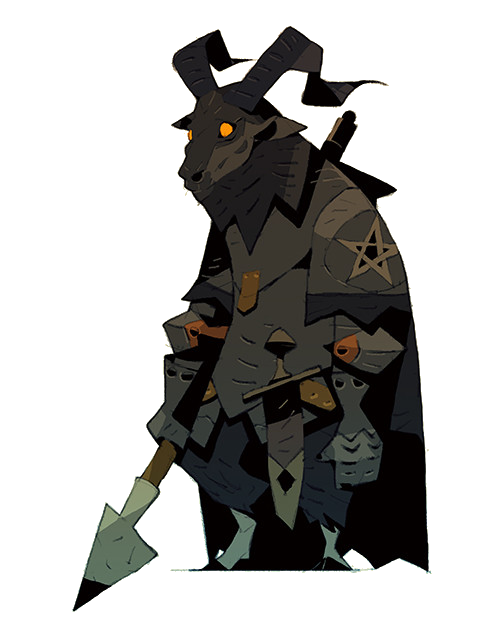
\includegraphics[width=0.47\textwidth]{03kins/img/11gat_knight.png}
\end{figure}

\newpage

\subsubsection{Noves Gat}
Acclimated to the highest mountains and deepest ravines, cliff gats are the most common of the horned kin.
Builders of the immense gat city-states, it's very rare to see a cliff gat not actively pursuing their craft.

\subparagraph{Ability Score Increase} Your time spent in civilization has given you a profound common sense and a general grasp on almost any subject.
Your Intelligence score is increased by 1.

\subparagraph{Gat Toughness} Your hit point maximum increases by 1, and it increases by 1 every time you gain a level.

\subparagraph{Expert Craftsgatship} Noves gats are renowned worldwide for their crafts, and even the untrained eye can recognize an item made by one.
You are an expert with the artisan's tools associated to your Craftsgatship trait.

The value of the item you produce in a strange mood is increased to 250,000 GP.
If you make a weapon, armor, or similar item, it is a +3 item.
Additionally, you must roll your Strange Mood wisdom saving throw twice at the beginning of every month.

\subsubsection{Bughna Gat}
In the year 102 AS, the army of healing invaded Ctereth's dwellings and plundered a great haul of qualar.
These qualar restored the minds of many gats, who became known as the bughna gats.
% While their minds were recovered, the habits they learned as lost ones have never truly been abandoned.

Bughna gats feel constrained in cities, and tend to abandon city-states at a young age, freely exploring the outside world.
% Despite their nature, gats are never truly free of their sense of community.
Bughna gats tend to travel in packs comprised by varied kins and ethnic groups.

\subparagraph{Ability Score Increase} Your balance and ability to walk on the steepest of hills is unmatched, and your Dexterity score is increased by 1.

\subparagraph{Fleet of Foot} Your base walking speed increases by 3 meters.

\subparagraph{See Them Coming} You have advantage on initiative rolls while in plains, grasslands, and any other open natural environment.

\subsubsection{Treb Gat}
While many of the gat lost ones were recovered, most of those who wandered off to the dead sea could never be found due to the toxic mist.
Here they became the Treb Gat, and eventually acquired qualar back via unknown means.

These gats are far removed from their calm origins, having to survive the harsh and hostile environment.
Treb gats have large and muscular bodies, large horns, and dirty, patchy hair.

\subparagraph{Ability Score Increase} Your restlessness knows no bounds.
Your Strength score is increased by 1.

\subparagraph{Size} Treb gats tend to be much larger than their common brethren, measuring between 160 and 200 cm and weighting between 90 and 120 kg.
Your size is still medium.

\subparagraph{Uncanny Brutality} While in combat, you are absorbed by a primal rage.
You have disadvantage on any attacks made with finesse, martial weapons without the heavy property, and ranged weapons.

\subparagraph{Hammering Horns} You are never unarmed.
Your horns are a melee weapon that deals 1d6 plus your Strength modifier as bludgeoning damage.

\subparagraph{Savage Attacks} When you score a critical hit with a melee weapon attack, you can roll one of the weapon's damage die one additional time and add it to the extra damage of the critical hit.

\subparagraph{Fell Mood} When you are struck by a strange mood, the need to craft an exquisite artifact is replaced by an unrelenting urge to kill.
You have to choose your prey from either a renowned hero, an ancient being, or a forgotten beast.

After the deed is done, you can craft a disquieting artifact from the creature's remains, following the normal rules of a strange mood.
All the other conditions of the trait remain the same, replacing the need to gather materials with the insatiable craving to hunt said creature.

\begin{figure}[!b]
    \centering
    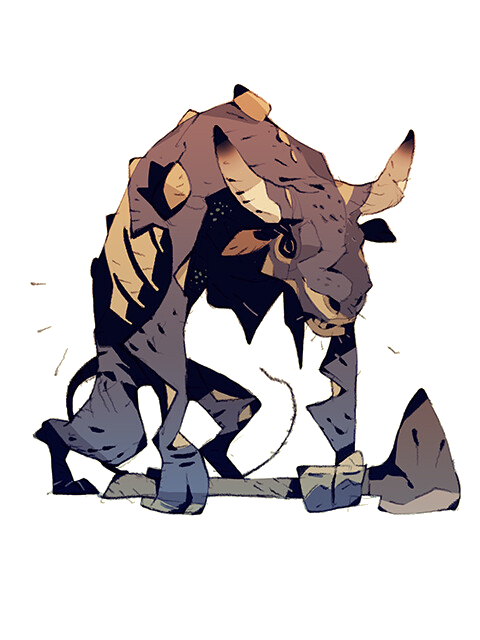
\includegraphics[width=0.48\textwidth]{03kins/img/11gat_treb.png}
\end{figure}
\end{linenumbers}

% !TEX root = ../main.tex
\section{Winged Kin} \label{sec::wingedkin}

\DndDropCapLine{Y}{es, sure, you can create a machine to}
\textit{glide.
You can even ride a creature to stay aloft.
But you will never truly fly.
No kin can tame the sky with such grace as the irds.
Trust me, if they weren't so humble as to live among us, constrained to the ground, we'd be building temples to venerate their graciousness.}

\hspace*{\fill} --- Josiah, priest from the church of Rhekesh.

Sequestered in high mountains, deep jungles, and hot deserts, the irds, sisz rlue, or winged kin are known to survive some of the harshest environments all around Yuadrem.

\subsection*{Beak and Feather}
From below, irds look much like large birds.
Only when they descend to roost or walk in the ground does their humanoid appearance reveal itself.
Standing upright, an ird might reach 2 meters tall.
They have long, narrow legs that taper to sharp talons.

Feathers cover their bodies, with their plumage typically reflecting the environment they develop in.
Their heads complete the avian appearance, being that of a parrot, hawk, or vulture.
Irds' arms have very long feathers, which allow them to fly with ease.
The three subraces of the irds are very distinct from each other.
This is due to the fact that they were created by three different ets, all in pursuit of a same goal, yet for different environments.

The winged kin are the only gendered species created by the tall kin.
Some time after reproduction, a female will lay one to three eggs and the couple will refrain from contact with others in their tribe, becoming extremely protective of their children until they reach maturity.

\subsection*{Sky Wardens}
Nowhere are the irds more comfortable than in the sky.
They can spend hours in the air, and some go as long as days, locking their wings in place and letting the thermals hold them aloft.
In battle, they prove dynamic and acrobatic fliers, moving with remarkable speed and grace, diving to lash opponents with weapons or talons before turning and flying away.

Once airborne, an ird leaves the sky with reluctance.
They sometimes forget or ignore vertical distances, and they have nothing but pity for those earthbound kins forced to live and toil constrained to the ground.

The ird are a tribal species, and its rare for a tribe to hold more than a hundred irds at once.
The only exceptions to this rule are the Krudzal and Kaldrathal, both large countries in the northern reaches of Yuadrem.
They are welcoming to traders and visitors in general, but generally don't allow members from other kins to be permanent residents within their territory, and frown upon guests who overstay their welcome.

Once tribes of irds settle in an area, they share a hunting territory that extends across an area up to 150 km on a side, with each tribe hunting in the lands nearest to their colony, ranging farther should game become scarce.
A typical colony consists of one large, open-roofed nest made of woven vines.
The eldest acts as leader with the support of a shaman.

\subsection*{Avian Mannerisms}
The resemblance of ird to birds isn't limited to physical features.
Irds display many of the same mannerisms as ordinary birds.
They are fastidious about their plumage, frequently tending their feathers, cleaning and scratching away any tiny passengers they might have picked up.
When they deign to descend from the sky, they often do so near pools where they can catch fish and bathe themselves.
Even when perched on a high branch or at rest in their mountaintop homes, they appear alert, with eyes moving and bodies ready to take flight.

Many winged kin punctuate their speech with chirps, sounds they use to convey emphasis and to shade meaning.
An ird might become frustrated with people who fail to pick up on the nuances; an ird's threat might be taken as a jest and vice versa.
Confinement terrifies the winged kin.
To be imprisoned by the cold, unyielding earth is a torment few ird can withstand.

\subsection*{Innate Curiosity}
Irds are naturally curious which, summed with their freedom of movement, leads to them being the ideal explorers and adventurers.
They use their large wings to travel to almost any place in the entirety of Yuadrem, and as such they've become a common sight in all its reaches.
Outside of their tribes, irds do enjoy living within other civilizations, and its rare to see a city or large settlement without at least one ird inhabitant.

% Winged kin tribes are accepting of their members leaving for indefinite amounts of time, and this is even encouraged in many communities.
% In fact, the population of a tribe is ever-changing, with the only constants being the eldest members and the shaman.
% This means that neighboring tribes have strong and healthy relations, each coming to aid the ones in need without question.
% Another consequence of their tendency to travel is the versatility of ird artisans, who integrate techniques from all around Yuadrem into their craft.

\subsection*{Ird Names}
Ird names separate into two main categories.
The first resemble their original language, Harualish, and include clicks, trills, and whistles to the point that other kins have a difficult time pronouncing them.
When interacting with other races, they may use nicknames gained from people they meet or shortened forms of their full names.

On the other hands, irds from Krudzal, Kaldrathal, and other civilized lands tend to speak Shanise.
Shanise is a language formed from the interaction of Harualish-speaking irds and Avshenese-speaking gats in the north.

An ird last name is usually simply ``son/daughter of'' followed by one of their parent's name.
Most irds admire their parents, and wear their last names with pride.

\paragraph{Harualish Ird Names} Aera, Aial, Aur, Deekek, Errk, Heehk, Ikki, Kleeck, Oorr, Ouss, Quaf, Quierk, Salleek, Urreek, Zeed.

\paragraph{Male Shanise Ird Names} Aden, Azat, Daneal, Dirkir, Eastean, Goker, Idrahin, Jakod, Jaldor, Jasin, Kuneit, Lutdzu, Nuretin, Nutlar, Rezat, Semir, Shasar, Tajik, Tenel, Tshasin, Unut.

\paragraph{Female Shanise Ird Names} Aise, Asutshan, De\~na, Dilsad, Dorun, Drinja, Eda, Gudlag, Gulden, Hazal, Iris, Katrin, Kisnet, Naina, Nerhe, Sehil, Selna, Sher, Solveag, Tedziye, Zainej.

\subsection*{Traits}
Your ird character has access to different abilities common to all subraces:

\subparagraph{Ability Score Increase} Your Dexterity score increases by 1, and your Wisdom score increases by 1.

\subparagraph{Age} Ird reach maturity by age 14, and don't usually live much longer than 150 years.

\subparagraph{Alignment} Ird have an inclination towards the red tide, which is supported by their adventurous lifestyle.

\subparagraph{Size} Ird are tall, and range from 1.70 to 2 meters.
They have thin bodies and hollow bones, weighing between 40 and 50 kilograms.
Your size is medium.

\subparagraph{Speed} You have a walking speed of 7.5 meters, and a flying speed of 15 meters.
To fly, you can't wear medium or heavy armor, carry heavy weapons, wield a shield or be encumbered.
Since you flap your arms to fly, you cannot use them to attack while flying.
You can use your versatile talons to hold and use simple weapons or spellcasting foci.

\subparagraph{Graceful Landing} Your years of living at great heights have taught you how to fall more gracefully.
You reduce the damage die for fall damage from a d6 to a d4, and you do not fall prone after taking falling damage, unless you are unconscious.

\subparagraph{Keen Senses} You are competent in the Perception skill.

\subsubsection{Qulbaba Ird}
Many irds can be found living in isolated tribes inside the jungles of Yuadrem.
In the east they live in Harual, and in the west in the Jenkashian empire.
Qulbaba ird have a face resembling that of a parrot, and their feathers' coloration depends on their gender.
Males usually have very brightly colored feathers, showing any combination of colors.
Females mostly have dull gray, brown, and dark green feathers, aiding their ability to hide in the jungle.

\subparagraph{Ability Score Increase} Your time gliding between branches and vines has augmented your flying capacity.
Your Dexterity score increases by 1.

\subparagraph{Bright Coloration} As a male, you are competent in the Performance skill.
Additionally, you have advantage on Charisma (Intimidation) checks made against creatures with an Intelligence score of 5 or less.

\subparagraph{Dark Feathers} As a female, you have advantage in Dexterity (Stealth) checks made in dim or dark light or in heavily forested areas.

\subparagraph{Strong Talons} You are competent with unarmed strikes, which deal 1d4 plus your Dexterity modifier as slashing damage on a hit.
Additionally, you have advantage of Strength (Athletics) checks made to climb any surface your talons could reasonably grip.

\subparagraph{Language} You know how to speak, read, and write Qualinese and one additional language of your choice.

\begin{figure}[!b]
    \centering
    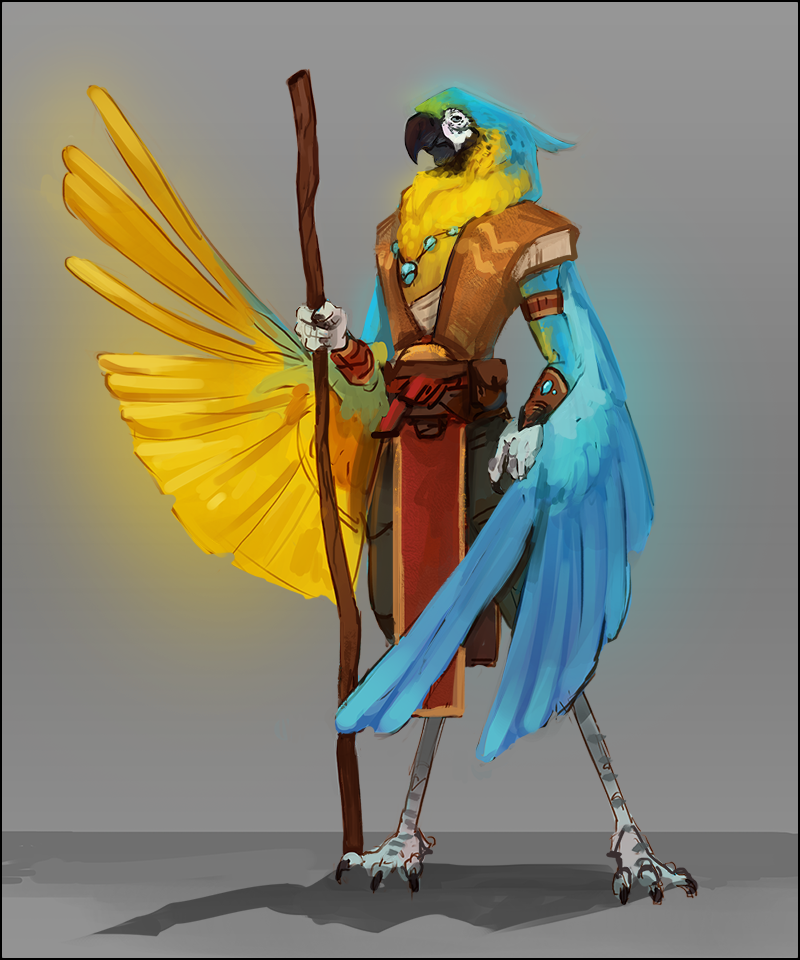
\includegraphics[width=0.48\textwidth]{03kins/img/12ird_qulbaba.png}
\end{figure}

% \newpage

\subsubsection{Thulkraka Ird}
Unlike their brethren, the Thulkraka tribes that settled on the many mountaintops of Yuadrem live their lives mostly constrained to the ground, and are only able to fly when the harsh mountain weather allows it.
They are thus bulkier than the average ird, and commonly are clumsy fliers due to their lack of experience.
Their faces are similar to that of hawks, and their feathers' coloration is bleak and cold, usually sporting white, gray, light blue, and brown colors.

\subparagraph{Ability Score Increase} Isolated from other races, you have been able to take the time to truly appreciate the calmness of the mountains.
Your Wisdom score is increased by 1.

\subparagraph{Bulky Frame} Your flying speed is reduced to 10.5 meters, but you can fly while carrying heavy weapons and/or wearing medium armor.

\subparagraph{Mountain Born} You're acclimated to altitudes up to 6,000 meters.
You're also naturally adapted to cold climates.

\subparagraph{Thulkrakian Descent} You are competent with smith's tools, as is tradition amongst your people.

\subparagraph{Language} You know how to speak, read, and write Shanise and one additional language of your choice.

\begin{figure}[!t]
    \centering
    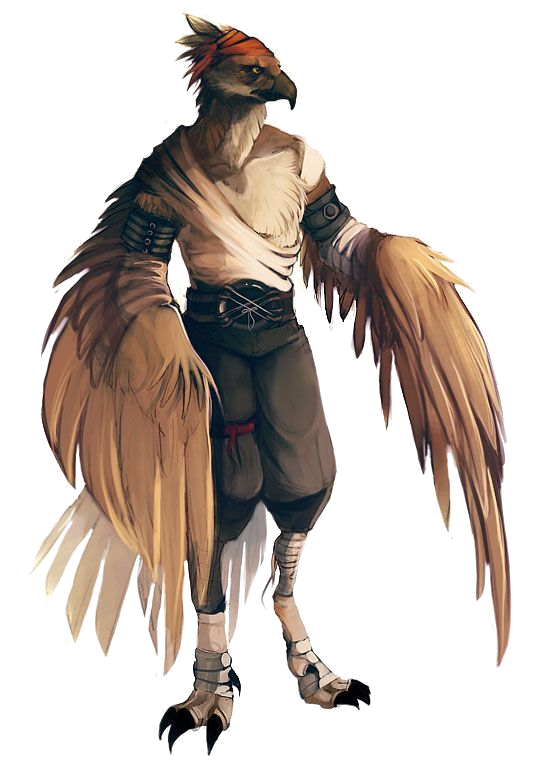
\includegraphics[width=0.47\textwidth]{03kins/img/12ird_thulkraka.png}
\end{figure}

\subsubsection{Dratl Ird}
Irds from the Dratl houses are known as ruthless ruffians, and are pariahs to the other winged kin subspecies.
They are known for constantly harassing the other ird tribes, as well as any who approach their territory.
The are collectively banned from entering any tribe from the other subspecies, and are usually unwelcome in towns and cities due to their bad reputation.

Nowadays, Dratl houses are scattered around the Zoedrem desert, mostly unorganized.
These are the remnants of the once great empire of Hulnar, disbanded in 591 AS.
Despite their lost grandness, they are still feared by the common people, and continue to fiercely protect their hunting grounds.

A Dratl ird's beak resembles that of a vulture, and their feathers are generally black, white, and red.
As a dratl ird grows up, their irises become noticeably white, while the sclera surrounding them turn into a bright red color.

\subparagraph{Ability Score Increase} Your time surviving in the harsh climate of the desert has given you an increased robustness.
Your Constitution score is increased by 1.

\subparagraph{Wing Flap} When you use the disengage action, you can choose to use another action to propel yourself upward a distance equal to half your flying speed.

\subparagraph{Bone Breaker} While flying, you can attempt to attack a creature with an eviscerating attack.
Using two actions, you can swoop down up to your flying speed towards a creature you can see, and make a melee weapon attack roll against it.
If the attack hits, it's a critical hit.
The attack is tiring, and you can use this trait only once per combat encounter.

\subparagraph{Language} You know how to speak, read, and write Zsekian and one additional language of your choice.

\begin{figure}[!b]
    \centering
    \includegraphics[width=0.47\textwidth]{03kins/img/12ird_dratl.png}
\end{figure}


\newpage

% !TEX root = ../main.tex
\section{Archer Kin} \label{sec::archerkin}

\DndDropCapLine{W}{hile traversing the jungle, be very}
\textit{conscious of your surroundings.
If you stumble upon fiber nests in the trees.
If you hear childlike voices screaming.
Run.
Run as fast as you can.}

\hspace*{\fill} --- Hedwyn's guide to the Chirping Wilds.

The archer kin are a species that resemble large marmosets, barely reaching 90 cm of height.
They share the brown coloration, white ears, and striped tail.
They are small creatures that inhabit the rivers, forests, and jungles of Yuadrem.

They are also known as marsets, or yuathe tle'thal rlue in Jantherlin.
Apart from their size, the other difference from marmosets is their back, which is protected by elongated, pointed quills, used as arrows.

Marsets are an asexual species able to lay eggs at necessity via a ritual after reaching maturity, only limited by the amount of dwellings and social constraints.

\subsection*{Misleading Appearance}
Marsets don't seem terribly intimidating at first glance.
They however have an unusual defense mechanism for driving away threats, which includes any unfortunate creature that disturbs their large arboreal colonies.

Each marset grows specialized quills from their back, with a smooth tip and a base with four flanges, like the fletching of an arrow.
In additional to making the marsets quite painful to grab, these quills are used as projectiles.

The little creatures construct their own bows, stripping bark from bendy twigs with their teeth to create the limbs, and harvesting spiderweb for the string.
The strands are rubbed together with sand, which is done to thicken the bowstring and reduce stickiness in the middle, creating a sophisticated weapon to launch quills at unlucky foes.

For shorter range, marsets also use hollow reeds to blow their quills as darts.
It's common for the smarter marsets to apply manure or poison to their arrows and darts, improving their deadliness.

\begin{figure}[!b]
    \centering
    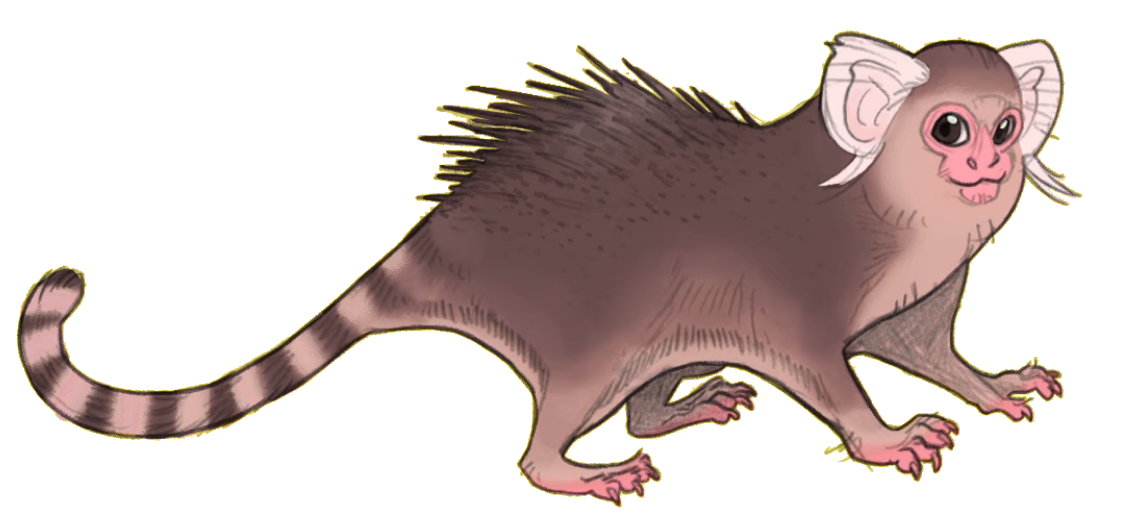
\includegraphics[width=0.48\textwidth]{03kins/img/13marset_brown.png}
\end{figure}

\subsection*{Arboreal Colonies}
The colonies that the marsets protect are just as complex as their weapons.
The structures are created from weaving grass and plant fibres around tree branches to create interconnected chambers.

A single colony can have up to 100 rooms and even more individuals living in it.
Rooms are assigned a specific function, and are passed down through related members of the colony.

Nursery rooms are where marsets lay their eggs, which they hatch into fluffy yellow infants.
Bedrooms are where the adults sleep.
Storage rooms are where food and various items are stockpiled.

In farming rooms they deposit a mixture of tough chewed leaves and bark, which then grows mushrooms.
The little marsets use these rooms to turn otherwise inedible foraged material into something tender and tasty.

While most marsets can be found in these colonies, some choose to live in cities and towns from other civilizations.
Here, they usually build interconnected rooms in trees, creating microcosms of the larger colonies.
Despite their fierceness in their natural environment, marsets are generally regarded as friendly creatures when encountered in urban settings.

\begin{figure}[!t]
    \centering
    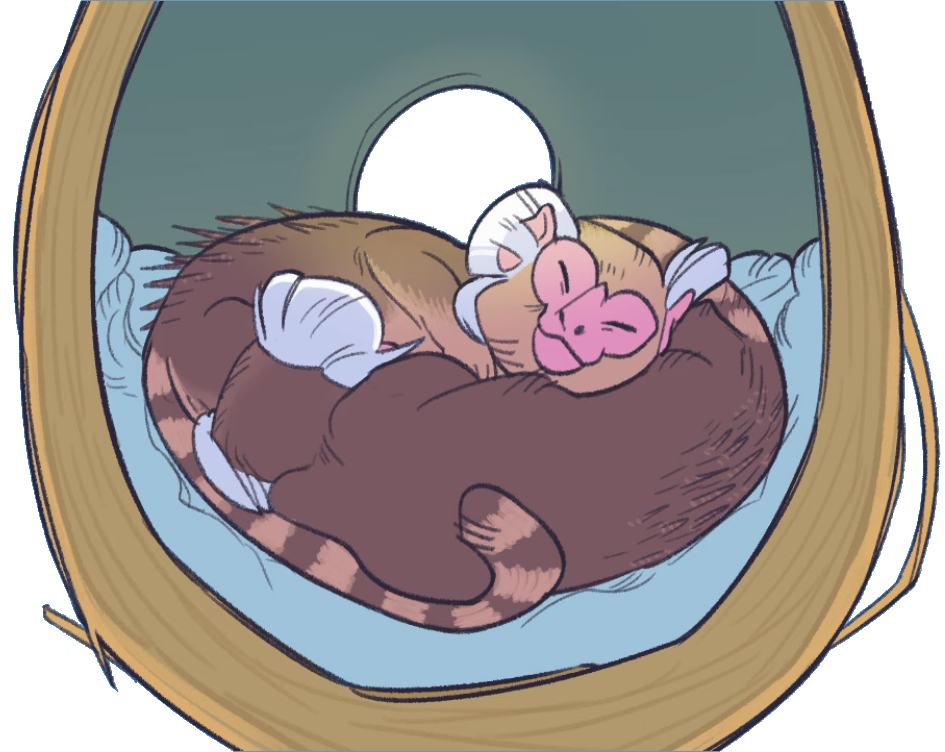
\includegraphics[width=0.48\textwidth]{03kins/img/13marset_room.png}
\end{figure}

\subsection*{Repetitive Language}
Marsets hatch from their eggs already able to speak a strange repetitive language, which is entirely regular and does not evolve.
This language --- known as Babazano --- can be spoken in one of two ways: soundlessly, with the communication happening through lip reading, or screamed as loud as possible, with no middle ground.
Despite this, a marset can learn other languages and not constantly scream at the top of their lungs, but they do tend to be loud speakers.

Babazano has only ten consonants.
All verbs use a single consonant as their root, so there's only ten verbs.
By repeating syllables they create new meanings, which makes their language very difficult to understand by the other kins, but for these little creatures it's no issue at all.
They hear or lip-read a word and instinctively know which one it is.

\subsection*{Exploring Opportunities}
Marsets don't usually set out on the adventurer's path for leisure, but rather out of necessity.
They will only leave their colonies to defend their communities or support their friends.
Only very few will set out to explore the wide world.
% For them, adventuring is less a career than an opportunity and more of a necessity.

\begin{figure}[!t]
    \centering
    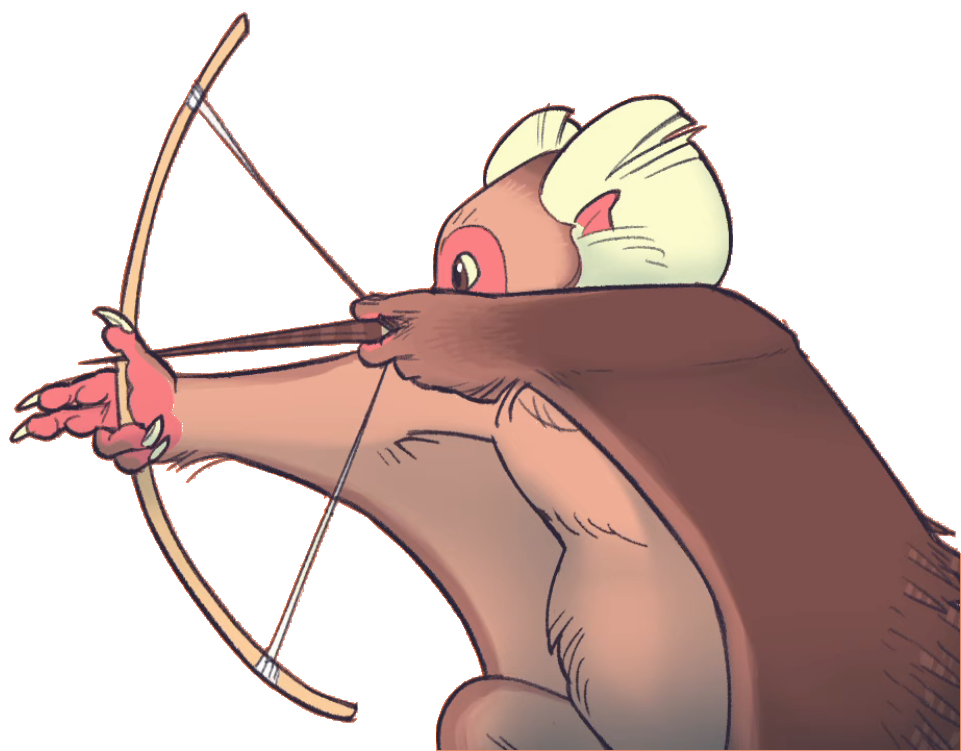
\includegraphics[width=0.48\textwidth]{03kins/img/13marset_bow.png}
\end{figure}

\subsection*{Marset Names}
Marsets assign names to each other based on distinctive features and accomplishment.
An individual marset will wear many names during their childhood, and when they settle on one is when they reach adulthood.
Due to the peculiarity of Babazano, it is a common for the other kins to call them by simple monikers, practice that the marsets despise.
% Most marsets don't particularly like this, and are very reluctant to accept a nickname given to them.

\paragraph{Names} Do Anana, Do Baba, Do Badada, Do Ebebebebe, Do Ezeze, Do Nono, Do Odododo, Do Uvu, Do Veve, Do Vovovo.

\subsection*{Traits}
Your marset character has a range of abilities based on its nature and community lifestyle.

\subparagraph{Ability Score Increase} Your Charisma score is increased by 2, and your Dexterity score is increased by 1.

\subparagraph{Age} Marsets has a short lifespan, reaching maturity by age 4 and not living much more than 50 years.

\subparagraph{Alignment} Marsets have a tendency towards helping others, specially in their communities, and are inclined towards the gold tide.

\subparagraph{Size} Marsets range from 75 to 90 cm.
They usually have a slender and agile frame, weighing around 20 kg.
Your size is small.

\subparagraph{Speed} Your base walking speed is 9 meters, and you have a climbing speed of 9 meters.

\subparagraph{Glider} You have loose flaps of furry skin between your arms and legs, which allow you to glide short distances at a speed of 9 meters per turn, as long as you are not wearing heavy armor.
You fall at a rate of 6 meters per turn while gliding, and suffer no falling damage on landing.

\subparagraph{Sneaky Nature} You have advantage on stealth checks in heavily forested areas.

\subparagraph{Natural Weapons} You are proficient with shortbows and blowguns, and can use your own quills as arrows or cut them to be used as darts.
Every day you can gather up to 10 quills from your back to be used in this fashion.

\subparagraph{Community lifestyle} Despite their loudness, marsets can be very compelling talkers.
You are competent in the Persuasion skill.

\subparagraph{Languages} You can speak Babazano from birth, and can lip-read the language.
You are also able to read and write Leafrunes, a special writing system designed to communicate simple messages to others of your kin.
Additionally, you know how to speak a language of your choice, but you don't know how to read or write it.

\begin{figure}[!b]
    \centering
    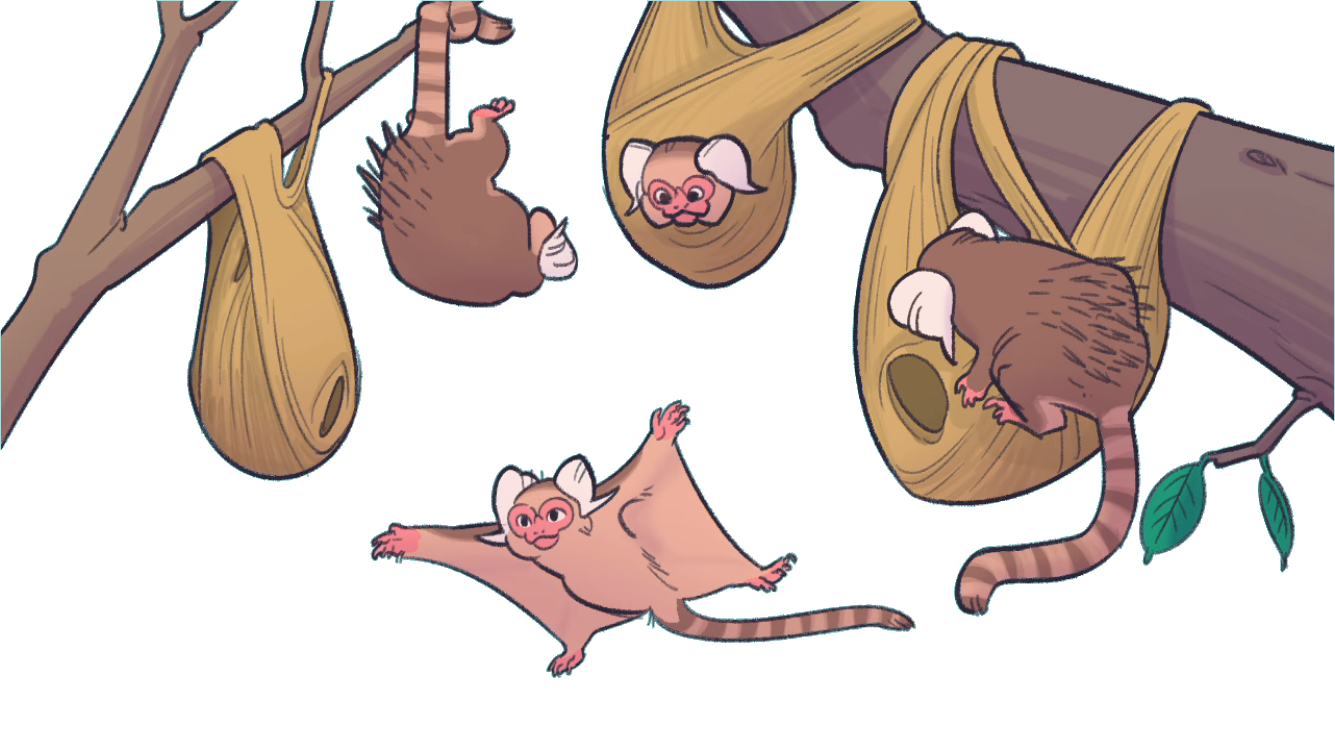
\includegraphics[width=0.48\textwidth]{03kins/img/13marset_colony.png}
\end{figure}


\newpage

% !TEX root = ../main.tex
\section{Dust Kin}
\begin{linenumbers}
\DndDropCapLine{T}{he light beckons, and you follow.}
\textit{As the light lead you once, now you are guided by enlightenment.
With each hidden truth you uncover, you learn more of what the world is, and how to secure your place in it.
Secrets are your power and your currency.
Seek them out, and guard them well.}

\hspace*{\fill} --- Ancient Moonborn saying.

Moody and perplexing.
Isolated and elegant.
Tough and passionate.
The ways in which one might describe the dust kin are many.
The dust kin, oths, or szua-tlekeloo rlue are a quiet species with a tendency towards nature and knowledge.
They're a solitary yet intimate creature with a penchant for nature and ritual.

\subsection*{Enigmatic and Uncanny}
While oths can be see as much as gats or irds around civilized lands, they are far more mysterious and reclusive than the two.
Often silent, oths have a reputation for being cryptic and thoughtful.
They tend to follow their intuition on a whim.

Oths usually travel with a large scroll in their backs made from their own fabric, which they protect with impermeable and resilient guards.
This scroll is a compendium of knowledge passed down through generations, and they add to it in key moments in their life.

The dust kin have large, heavy forewings that hang around their humanoid bodies like cloaks, which hide a shorter and more delicate set of hindwings behind them.
They have two sets of arms, one above the other.
The upper pair is strong and long, while the lower one is weak, and mostly left for secondary tasks.
Their feet have three fingers and their arms have four, with one being an opposable thumb.
They have an insectoid face with antennae and compound eyes.
Their body is covered in a short, fluffy hair which is usually of a very pale brown color.

\subsection*{Long Tempers}
Through generational learning, oths are wise and prudent creatures from a very early age.
Many chase intellectual or mindful pursuits, becoming librarians and philosophers.
They pontificate on the nature of life and knowledge.
Most think that the oth are naturally intelligent, and take their opinions with very high regard.

While most dedicate to cultivating their cognition, some decide to live their lives in adventure.
They nurture their minds with experience, acquiring knowledge via facing the challenges of the world.

A common thread throughout the race is that they are slow to anger.
Regardless of culture, it is instilled in them as early as the larval stage.
Life is too short to be spent in anger or frustration.

\subsection*{Cycle of Resurrection}
An oth knows when their natural death approaches, and faces it peacefully.
When they are near their death, they say their goodbyes and withdraws from civilized society.
The oth then pilgrimages towards a cavern or secret place they designated during their lifetime.

On arrival, the oth blocks all but one entrance to this sacred place, and lays ten to twenty eggs in a bed of silk during fall.
They then spend their time gathering foodstuffs and lining the walls, floor, and roof with silk, providing a safe environment for their descendants to develop in.
The oth also uses this time to finish writing their compendium of knowledge in their scroll, developing it until its ready to be passed on to their strongest descendant.

At the last week before the break of summer, the oth closes the last entrance to its sacred place, engulfing it in total darkness.
And they wait.

At some point during summer, the eggs hatch for their parent to greet and nourish their newborn larvae.
They dying oth hands qualars to their progeny, teaching them their language and the way of the world.
Along with this they pass on the tenets of their culture.
The parent eats no more than a grain of rice per day, and refrains almost completely from liquids.

Six months after hatching, the younglings go through the process of pupation, remaining as pupa for a year.
The parent uses this time to drink an embalming fluid, and mummifies themselves in silk.
They slowly lose their sentience, peacefully drifting into non-existence.

After hatching, the oths pay tribute to their now dead parent, and re-seal their cradle.
The first place they see becomes their parent's final resting place.
The oths then travel together, forming a small familiar tribe which lasts until they reach maturity.
While the members of the family may part ways, the bond they share is never truly broken.

\subsection*{Educated by Experience}
Due to the way the oths spend their youths, they are generally very wise from a very young age, blessed with the knowledge of the previous generations.
However, it's in an oth's nature to cultivate this wisdom with a contemporary and personal viewpoint of the world.
It's rare to see an oth not spending much of their youth travelling for knowledge and wisdom.
% The dust kin is also very concerned about the preservation of nature, and are experts at recording its sights and dwellers in great detail.

\subsection*{Oth Names}
In oth culture, the parent is assigned the task of naming each of their children in their larval stage.
These names will often change at the whim of the parent, not becoming official until pupation.
Their names are often difficult to pronounce by the other kins, and most don't mind being called by a nickname for simplicity.
The dust kin doesn't use family names, recognizing their relatives by sight alone.

\paragraph{Names} Adz'kt, Andle, Axa, Bixi, Chch, Chith, Daph, Fen'kt, Fl'ka, Fra, G'zigg, Gl'rik, Hadae, Iitus, J'llkx, Kl'il, Lenna, L'kpha, Mlf, N'kakt, Riz, Scelkt, Sud'kx, Thm, Timpth, Zkx.

% \begin{table*}[b]%
%     \begin{DndTable}[width=\linewidth, header=Oth Silk Armor]{lXXXX}
%         \textbf{Armor} & \textbf{AC} & \textbf{DC} & \textbf{Time taken} & \textbf{Cost} \\
%         Silk Armor                & 11 + Dex mod     & 10 & 1 week   &    -    \\
%         Reinforced Silk Armor     & 12 + Dex mod     & 15 & 2 weeks  &   10 GP \\
%         Exquisite Silk Armor (+1) & 12 + Dex mod + 1 & 20 & 1 month  &  100 GP \\
%         Excellent Silk Armor (+2) & 12 + Dex mod + 2 & 20 & 6 months & 1000 GP
%     \end{DndTable}
% \end{table*}

\subsection*{Traits}
Your oth character has the following set of skills, based on its customs and ancestry.

\subparagraph{Ability Score Increase} Your Intelligence score increases by 2.

\subparagraph{Age} An oth will go through three stages of growth: eggs, larvae, and pupa.
This development takes in total about two years.
In terms of maturity, they emerge from their pupa as adults, but reach full size at about ten years of age.
Oths live to be around 80 years old.

\subparagraph{Alignment} Oth tend to stray from extremes, most often remaining neutral in conflicts as long as there is no direct danger to themselves or those close to them.
The oths passion for wisdom leads them to the blue tide.

\subparagraph{Size} Oth typically range from between 135 to just under 180 cm.
Your size if Medium.
You are impressively lightweight for your size, weighing around 45 kg.

\subparagraph{Speed} Your base walking speed it 9 meters.

\subparagraph{Clumsy Flight} Once per short rest, you can fly with a speed of 6 meters for a number of rounds equal to your Constitution modifier plus 2, with a minimum of 2 rounds.
You cannot use this feature while you wear heavy armor or carry heavy weapons.

\subparagraph{Darkvision} Due to your nocturnal heritage you have a good sense of vision in the dark.
You can see in dim light within 18 meters of you as if it were bright light, and in darkness as if it were dim light.
You can't discern color in darkness, only shades of gray.

\begin{figure}[!t]
    \centering
    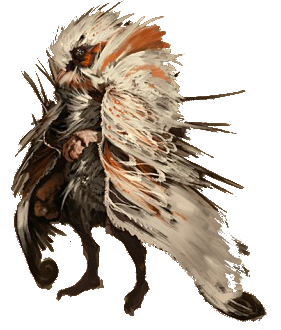
\includegraphics[width=0.48\textwidth]{03kins/img/14oth_white.png}
\end{figure}

\subparagraph{Four-armed} You have a pair of weaker secondary arms that can be used to hold small objects and perform simple tasks.
You cannot use these arms to wield weapons or shields and Strength checks using them are made with disadvantage.
Due to your unique form, armor may need to be specially made, leading to additional costs.

\subparagraph{Languages} You know how to speak, read, and write Shamabic and one other language of your choice.

\subsubsection{Moonborn}
The moonborn are the most common of the oth.
They prefer shady areas, and tend to live their lives in such places.
They have been properly schooled under the light of the moon as oth tradition dictates, and many can be found in darkened libraries during daytime.

As their name suggests, moonborn have a special affinity for the moon, and can even feed off its light.
They travel at night and hide during the day, and most carry a specially designed tent that blocks all incoming sunlight.

\subparagraph{Ability Score Increase} Your Wisdom score is increased by 1.

\subparagraph{Light Sensitivity} Moonborn grow away from the sun.
You are vulnerable against radiant damage.
You have disadvantage on attack rolls and Wisdom (Perception) checks that rely on sight when you, the target of your attack, or what you are trying to perceive is under direct sunlight.

\subparagraph{Sensitive Antennae} Using your specialized antennae, you have advantage on perception checks that rely on smell.

\subparagraph{Lunar Studies} You are competent in the Religion and History skills.

\subparagraph{Moon Magic} You know the Light cantrip (page \pageref{spell::light}).
When you gain your third hit die, you learn the Faerie Fire spell (page \pageref{spell::faeriefire}), which you can cast once per day.
When you get your fifth hit die, you learn the Glitterdust spell (page \pageref{spell::glitterdust}), which you can cast once per day.

Intelligence is your spellcasting modifier for these spells.

\subsubsection{Chu'ash Kin}
The chu'ash oths are a subculture that differentiate from the rest by their curious and reckless nature.
Weaker than their siblings, they are born a summer too late, and never get to meet their parent.
They are instead cared for by their older siblings, and are the younger members of their familiar tribes.

To most, a chu'ash oth seems perpetually disorganized and distracted, which leads to the belief that they have a lower intelligence to the other of their kin.
In truth, the chu'ash have a unique perception of the world.
They are able to interpret information in a unique way, allowing them to see possibilities other cannot.
Born with an untamed intelligence, the chu'ash oth has an affinity to find the hidden patterns of the world.

\subparagraph{Ability Score Increase} Your Charisma score is increased by 1.

\subparagraph{Fated} Whether luck of a guiding presence, you always seem to find your way.
Once per day you can choose to reroll an attack, skill check, or saving throw.
You can decide to do this after the roll, but before the outcome of the roll has been determined.

\subparagraph{Touched} You know the Dancing Lights cantrip (page \pageref{spell::dancinglights}).
When you gain your third hit die, you learn the Color Spray spell (page \pageref{spell::colorspray}), which you can cast once per day.
When you get your fifth hit die, you learn the Blur spell (page \pageref{spell::blur}), which you can cast once per day.

Charisma is your spellcasting modifier for these spells.

\subsubsection{Sunstruck Oth}
While most oths follow the circle of resurrection to the letter, there are a few who choose to ignore it.
They lay their eggs under direct sunlight, and their larvae quickly lose their fragile hindwings.
Unrepairable, their wings stay atrophied and shriveled thorough their lives.

These oths are known as the sunstruck, and they've earn a reputation of unpaired hardiness and resilience.
The clans of Shief and Zmiva cherish this attribute, and consciously molt in lit areas to engender it.

\subparagraph{Ability Score Increase} Due to your hardiness, your Constitution score is increased by 1.

\subparagraph{Sunstruck Birth} You lose your \textbf{Clumsy Flight} and \textbf{Darkvision} traits.

\subparagraph{Photosynthesis} While you need water like any other creature, you don't need to eat to gain sustenance.
You can choose to instead collect light with your wings via photosynthesis.
Each day, you must spend two hours with your hindwings exposed to sunlight, or four hours to moonlight to be properly well fed.

\subparagraph{Sunstruck Resilience} You are competent in the Survival skill.

\subparagraph{Vertical Takeoff} As an action, you can use your powerful frame and knowledge of thermals to propel yourself upward a distance equal to double your movement speed.
This technique is used by the Shief scouts to survey the desert around them in search of food or predators.

\subparagraph{Slow Fall} While useless for flight, your shriveled wings allow you to slow your fall.
When falling, you can use an action or reaction to lift your wings using your second pair of arms to slow your descent.
You continue to fall gently at a speed of 9 meters per round, taking no fall damage when you land.
You cannot use this trait if you are wearing heavy armor or are encumbered.

\end{linenumbers}

\newpage

% !TEX root = ../main.tex
\begin{linenumbers}

\section{Moss Kin}\label{src::naenk}
\DndDropCapLine{W}{e thought they were mindless}
\textit{savages, but they know what they're doing.
They ain't hiding from us, they're preparing an attack.
They're studying our movement, figuring out our tactics.
They're hunting us.}

\hspace*{\fill} --- Grigor, Drejeck expedition leader.

The moss kin, or naenks, are moss creatures that hunt in the dark, warm, and wet jungles of Drejeck.
They hunt for sustenance and to gather fresh corpses.

\subsection*{Short and tangled}
The naenks are mostly known for their strange reproduction.
They spawn from the corpses of hunted humanoids exposed to the nanust spores of the great tree Tekatsae.
The spores grow into moss, merging with the corpse's muscle tissue and flesh.
After a period of about two months, the corpse rises again, this time in the shape of a naenk.

The moss kin are a thin race.
Their height varies considerably, but they usually are slightly smaller than their birth corpse.
Their bodies mock a humanoid shape, made up by a mix of bone, flesh, vine, and moss.
They protect their fragile interior with thick layers of flora.

Naenks typically have a healthy green coloration, but their skin can be of any mix of colors between moldy blue, dark orange, gray, and even white.
Their eyes are of a white or yellow color, where a thick fluid hides their pupils from the eyes of others.

Naenks naturally grow leaves and mossy tendrils at the top of their heads that resemble hair, which can be of a black, brown, or yellow color.
They typically arrange this mock-up of hair in a simple topknot.

% Due to the duality of their bodies, naenks follow a very particular diet.
% They needs to regularly consume meat in order to maintain the corpse inside them.
% They also feed off nutrients from the soil to feed the vines and plants that surround this corpse.

\subsection*{Tribal Communities}
% A naenk also assists their communication with rhythmic tapping on their body and using a complex system of gestures.
% Apart from these, they can also speak telepathically when close to tsaneks or sovereigns, aiding their communication.

Naenks are organized in tribal units called bands.
Each band is lead by the strongest naenk, the chief, who commands alongside a tsanek shaman.
Naenk chiefs bear special spores that can be used to infect beasts in a manner similar to the Tekatsae tree.
They spawn a bestial moss creature known as nuen with this spores, who acts as a pet or mount to the chief.
When a naenk travels alone, it is usual for them to also grow these spores as well.

Naenks build and craft very little.
Their gear is simply what they loot, and they build simple structures by imitation.

Due to their odd appearance and homicidal reproduction, naenks are seen as something to fear.
They however are very bold, yet fear the strangest things due to superstition.

Strangely, if they remain inside Drejeck, a naenk will not need to carry a qualar to remain sentient.
This ability only works inside of the jungle however, and they quickly lose their sentience if they leave their home without a qualar.

\subsection*{History and Legends}
To become part of a band, an infant naenk needs to go through a unique ritual.
A tsanek shaman removes their thyroid cartilage, who then punctures an odd pattern of holes into it.
After fitting small wooden tubes into these holes, the cartilage is put back into its original place.
After healing, the naenk's voice becomes accompanied by an eerie whistling noise, which is used for communication and intimidation.

Later, the naenk joins a group of other would-be-warriors.
They leave the safety of the tribe to travel to the northern lakes of Drejeck.
In there they must hunt a whowie, a huge frog-like beast that preys on the moss kin.

While they are fierce beasts, whowies are very afraid of the naenks' whistling, aiding the latter in combat.
If the group succeeds, the bravest of the group will cut the whowie's tongue.
Upon returning to the village, the group becomes a new band, and the owner of the tongue becomes the band's chief.

\subsection*{Call to Adventure}
A naenk rarely leaves the Drejeck jungle in which they are born.
However, many reasons can spark the need for a naenk or an entire band to abandon their home.
A band may leave engaging on a quest, as commanded by Tekatsae itself, or in shame after failing in one.
The most common bands abandoning the tribe are those that failed on their initiation rite, culled by the vicious whowie.

While in groups they may be savage, individual naenks are not completely insensitive people.
It is not too rare for a naenk to abandon their tribe in search for a different life.
Discontent with their chief, tiredness from their class system, or mere curiosity of the outside world count among the most common reasons for a naenk to travel by themselves.

% Only known among the naenk and the tsanek is the fact that a huge qualar lies inside the tree itself, which imbues the colossal plant with sentience.
% How this object ended up inside the tree is unknown, but it is thought among them that the tall one cter-rheth is looking to recover it.
% Due to the fact that the kin can't reproduce by themselves, they protect the tree with their lives and, under normal circumstances, won't allow anyone to even approach it.

There is an old legend of a courageous band that will one day sneak into Ctereth's lair and steal a huge bounty of qualars.
These will be used to grow a second tree, brother to Tekatsae, improving the kin's survival by a large margin.
Many groups have tried to become this band of legend, but none has returned thus far.

\begin{figure}[!b]
    \centering
    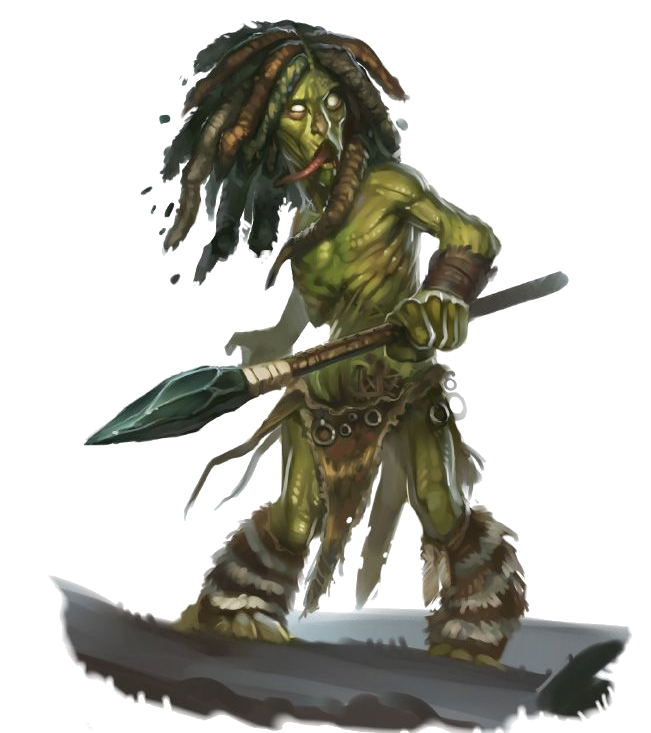
\includegraphics[width=0.48\textwidth]{03kins/img/15naenk_warrior.png}
\end{figure}

\subsection*{Naenk Names}
Naenks are born without names, and usually remain nameless most of their youth.
They reach social adulthood by earning a name, which is done either by becoming a warrior or accomplishing a major deed.

Many naenks live their whole lives unnamed.
While most accept this reality and become gatherers, it is not uncommon for the nameless to self-exile out of shame or discontent.

Knaenese is a very hard language to pronounce, so it's common for people of other kins to call naenks by a nickname or a simpler version of their name.

\paragraph{Names} Gantauda, Gesunt, Gunsedant, Hanhant, Hanseek needa, Hantadage, Huntge, Keena, Kegunseeda, Knaetseeknan, Knandage, Knudu, Kueqan, Nade, Naekuntge, Nega, Nelati, Seetun, Tsaegae, Tsege, Tsehant, Ukena.

\subsection*{Traits}
Your naenk character has an assortment of abilities, relating to their nature and surroundings.

\subparagraph{Ability Score Increase} Your Dexterity score increases by 2.

\subparagraph{Age} A naenk typically lives at most 30 years.
They are naturally mature right after being born and usually take less than a month to adapt to their society.

\subparagraph{Alignment} Naenks are organized creatures, used to following the rules of their communities.
Most tend towards the silver tide, especially those who haven't gained a name yet.

\subparagraph{Size} The moss kin come in very varied shapes and sizes.
They stand a tiny bit smaller than their birth corpse, but weight about half.
Your size and anatomy varies greatly depending on your birth corpse. \label{kin::naenk.size}

\subparagraph{Speed} Your base walking speed is 9 meters.

\subparagraph{Dual Nature} You are both humanoid and plant.

\subparagraph{Naenk claws} Because of your sharp claws, you have a base climbing speed of 9 meters.
In addition, your claws are natural weapons, which you can use to make unarmed strikes.
If you hit with them, you deal slashing damage equal to 1d4 + your Strength modifier, instead of the bludgeoning damage normal for an unarmed strike.

\subparagraph{Eat by Osmosis} While naenks prefer to eat meat by nature, you can mostly live off nutrients from the ground.
When in fertile land, you only need to eat once per week.
You can also eat more often if you choose to do so.

\subparagraph{Languages} You can speak, read, and write knaenese.
You can also speak, read, and write other language of your choice, but your pronunciation leaves much to be desired.

% Despite their lack of lips, the moss kin does speak a language, which is named Knaenese.
% Knaenese is a very simple, accommodating to their impaired speech.
% While a naenk can learn other languages, their pronunciation usually leaves much to be desired.

\subparagraph{Subraces} Naenks are most easily separated by their home - Gannag or Na'ane.

The most common of their kin, Gannagian naenks are the members of the tribes that surround the Tekatsae tree.
They have a very strong sense of community and an excellent capacity to work as a team.
Any one naenk will easily give their life without second thought for their people and for their way of life.

While all naenks are capable fighters, Gannagian naenk take on different jobs to fulfill different tasks.
The most common of these are the warriors, the hunters, and the gatherers.
Your subrace traits depend on which of these roles you take.

\subsubsection{Gannagian Warrior}
\subparagraph{Ability Score Increase} Your Strength score increases by one.

\subparagraph{Moldy Companion} As part of a long rest, you may contaminate a recently deceased beast with nanust spores.
To do this, you must succeed on a medicine ability check of DC 8 + the creature's number of hit dice.
If you succeed, the spores will settle into the beast, and the corpse rises as your nuen at the end of the long rest.

The nuen has the stats, abilities, and actions of the original beast, but its hit points and hit dice are cut in half.
It acts on its own volition and on its own initiative turn, but you can use an action to issue an order to it, which it follows to the best of its abilities.
It also gains the Plant Camouflage trait (page \pageref{trait::plantcamouflage}).

When travelling with one or more gannagian warriors, only the naenk with the highest Wisdom score can use this trait.

\subparagraph{Combat Training} The damage die of your claws is increased from a d4 to a d6.
Additionally, you can choose to add your Dexterity bonus rather than your Strength bonus to your attack and damage rolls.
% Trained and proficient in combat, you know the first rank of the \textbf{Armed Fighter} feat (page \pageref{feat::armedfighter}).

\subsubsection{Gannagian Hunter}
\subparagraph{Ability Score Increase} Your Constitution score increases by one.

\subparagraph{Plant Camouflage} You have advantage on Dexterity (Stealth) checks you make while in any terrain with ample obscuring plant life.

\subparagraph{Hunter's Guts} You are competent in the Survival skill.
Additionally, your base climbing speed is increased to 9.

\subsubsection{Gannagian Gatherer}
\subparagraph{Ability Score Increase} Your Intelligence score increases by one.

\subparagraph{Darkvision} Gatherers spend most of their life recollecting fungus underground, which provides you with an increased awareness in the dark.
You can see in dim light within 18 meters of you as if it were bright light, and in darkness as if it were dim light.
You can't discern color in darkness, only shades of gray.

\subparagraph{Seedspeech} Through sounds and touch, you can communicate simple ideas to living plants, and are able to interpret their responses as simple language.
Plants do not perceive the world in terms of sight, but most can feel differences in temperature, describe things that have touched them, as well as hear vibrations that happened around them (including speech).

\subsubsection{Na'anian Naenk}
Among the naenks that grow disillusioned with their tribes, many choose to pack their possessions and leave.
Among these self-exiled naenks, most usually choose to join the neighboring nation of Na'ane to live with their tsanek brothers.

These naenks drink a special beverage upon arrival known as nahan cooked by the nations sovereigns.
% NOTE: Nahan literally means "I-water" in Knaenese.
Nahan weakens the bond of the naenk with the Tekatsae tree, forcing them to attain a qualar to remain sentient.
% As a side effect, it also extends the naenk's life, pushing it to about 50 years.

\subparagraph{Ability Score Increase} You are learned the way of the tsaneks, and your Wisdom score increases by one.

\subparagraph{Rapport Spores} Your time among the tsaneks has allowed your body to adapt, and fungal growths are found all around your body.
You can extend rapport spores in a 4.5 meter radius as an action.
These spores go around corners and affect any creatures with an Intelligence score of 2 or more that aren't undead, constructs, or elementals.
Creatures affected by the spores realize the effect immediately, but those outside of range cannot notice it.
Affected creatures can communicate telepathically with one another while they remain within 9 meters of each other.
The effect lasts for 15 minutes.

\subparagraph{Noxious Spores} When a creature touches or hits you with a melee attack, you can choose to secrete noxious spores as a reaction.
The creature takes 1d6 poison damage if it isn't undead, construct, or elemental.
You can use this skill a number of times equal to your Constitution modifier (minimum of 2).
After expending all uses, you can't use this trait again until you complete a short rest.

\begin{figure}[!b]
    \centering
    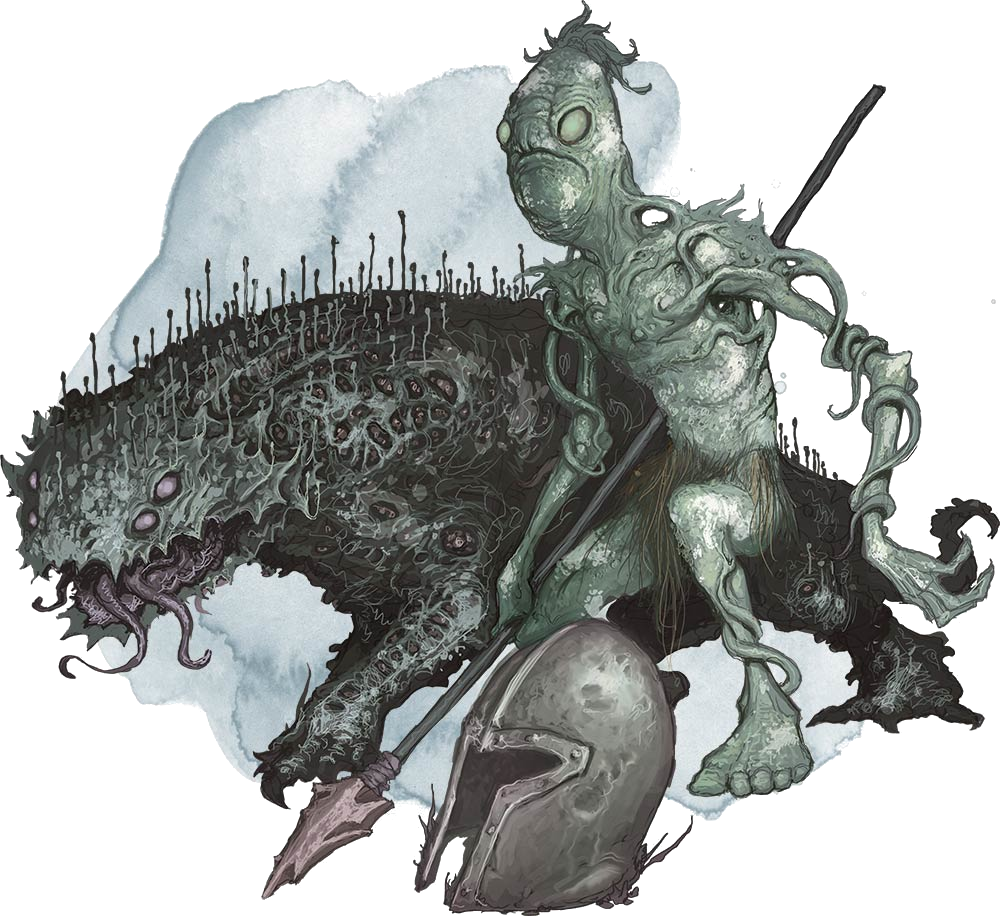
\includegraphics[width=0.48\textwidth]{03kins/img/15naenk_nuen.png}
\end{figure}

\end{linenumbers}

\newpage

% !TEX root = ../main.tex
% TODO: GENERAL CHECKUP NEEDED

\section{Fungal Kin}
\begin{linenumbers}
\DndDropCapLine{I}{ done seen some things down there.}
\textit{There be cities grander than any of gat's make, holdin' creatures stranger than the harrowing immensity isself.
There be ungodly abominations that weren't never meant to see the light o' day.
And there be... there be mushrooms! An entire city of mushrooms!}

\hspace*{\fill} --- Blim, the Na'anian chronicles.

% TODO: MOVE TO TSANEK SECTION!

% Apart from its chief, every unit has a designated tsanek shaman.
% This tsanek is mainly in charge of communicating with the other tsaneks in faraway places, aiding in the coordination of the tribe as a whole.
% Apart from this and other ceremonial tasks, the shaman acts as a normal member of the unit.

% The highest ranking members of their society are the sovereigns and elder sovereigns, who are tsaneks that reached their final stage of development.
% The former are huge mobile tsaneks that take root in strategic positions in Drejeck to establish their complex communication network.
% The latter are the eldest in the tribe, and merge with Tekatsae itself.
% They directly speak to the tree, communicating its wishes to the sovereigns and shamans via their root network.

Also known as tsaneks in the naenk tongue, the fungal kin is a species of intelligent fungi creature that inhabit swamps, forests, and caverns.
They are commonly seen in the jungle of Drejeck, as members of the tribes near the tekatsae tree.
Like the naenks, tsaneks grow from the tree itself, starting out as small russet-colored fungi in the tree's base and exposed roots, until they're able to grow legs and emerge.
Unlike the naenks, the fungal kin are capable of reproducing by themselves, and it's very common to find independent tsanek communities in the darker reaches of Yuadrem.

Tsaneks generally deplore violence, and only attack when provoked.
If approached peacefully, they gladly provide shelter or passage through their colonies.

\subsection*{Tribal Life}
Most tsaneks belong to the tribes of Drejeck, filling the roles of shamans and diplomats that the naenks are less likely to fulfill due to their violent nature.
They are considered above their mossy companions in their social circles, and are generally treated with respect among them.

When a tsanek reaches 100 years, it is put through the rite of growth.
The tsanek must ceremoniosly consume a mixture of the sap of tekatsae, wyvernroot, and water of the boiling river. % Wyvernroot is a strong poisonous plant native to Drejeck.
Next, it must enter a chamber of awareness, which are small caverns below tekatsae.
The tsanek is only left out after a month in isolation.
Most of the tsaneks that go through this ritual die, and are consumed by tekatsae, bringing them back to the tree.
The ones that don't become the highest ranking members of their tribal societies: Sovereigns.
Tsanek sovereigns are large, malformed creatures that reign over the tribes.
They are the only creatures capable of directly speaking with tekatsae, and thus are the only that can communicate its wishes to the tribes.

\subsection*{Circles and Melds}
Many tsaneks, feeling unprepared, leave the tribes before this ritual.
Usually many more of their species follow them to start independent communities as exiles.
Over a timeframe of 300 to 400 years, the eldest from these colonies naturally grow to become sovereigns themselves, presiding over many social groups called circles.
A circle consists of twenty or more fungal kin that work, live, and meld together.

Melding is prohibited in the Drejeck tribal communities, but is a regular practice in these circles.
A meld is a form of communal meditation that allows tsaneks to transcend their sometimes dull existence.
Their rapport spores bind the participants into a group consciousness, inducing a shared dream that provides entertainment and social interaction.
Tsaneks use melding in the pursuit of higher consciousness, collective union, and spiritual apotheosis.
They can also use their rapport spores to communicate telepathically with other sentient creatures.

\subsection*{Tsanek Reproduction}
Like other fungi, tsanek reproduce by mundane sporing.
They are the only race that can retain their sentience without qualar, but if their spores grow without the influence of tekatsae or a particularly old sovereign, the sprouting quickly becomes feral, unable to retain sentience.
Due to this, tsaneks carefully control their spores' release.

Tsaneks are known to feel very little connection to their offspring.
Among the tribal tsaneks, the children of their species are taken care of by a few tsanek designated as the spore-caretakers.
Among the exiles, child rearing becomes a responsbility shared by the entire circle.
It is rare if young tsaneks can even identify their parents.

\subsection*{Call to Adventure}
While many tsanek are needed in the tribes near tekatsae for managerial tasks, it is not unusual for some to travel the globe to learn.
Most focus their study on the qualar and cter'rheth, bringing this knowledge back to their tribes.

Cavern tsaneks regularly travel the many caves below Yuadrem, and some even settle outside of their colonies, most usually in dark gat cities.
Some have founded libraries, laboratories, and monasteries, usually along oths, and dedicate their lives to research and education.

\subsection*{Tsanek Names}
Due to the fact that tsaneks have no verbal language, their names are most appropriately translated as physical descriptions of a particular individual.

\paragraph{Names} Bolete, Brownback, Buttonhead, Greenfoot, Morel, Mossy, Portabelt, Puffball, Redstem, Soft-Step, Stinkhorn, Toad.

\begin{figure}[!t]
    \centering
    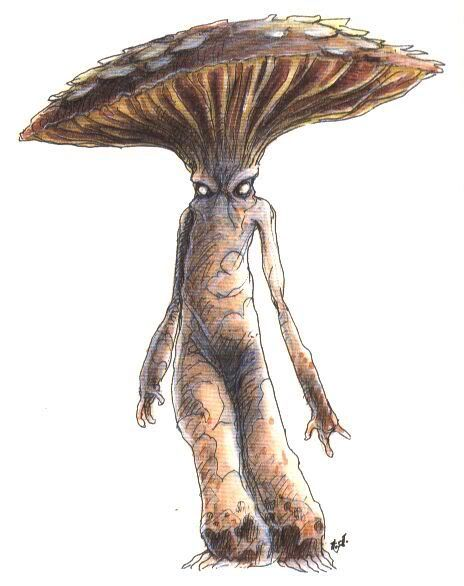
\includegraphics[width=0.48\textwidth]{03kins/img/16tsanek_individual.jpg}
\end{figure}

\subsection*{Traits}
Your tsanek character has a diverse set of skills based on its nature and role on society.

\subparagraph{Ability Score Increase} Your Wisdom score increases by 1, and your Constitution score increases by 1.

\subparagraph{Size} A tsanek grows to a wide variety of heights and builds, with the most common being stocky and measuring about 1.9 meters in height, weighing around 65 kg.
Your size is medium.

\subparagraph{Speed} Your base walking speed is 9 meters.

\subparagraph{Age} Individual tsanek are not known to die of old age, and the most elder can live to become a sovereign of one or more circles, living indefinitely longer.
Sproutings take a long time to fully mature, but it's a continuous process and even the oldest tsaneks seem to continue growing, albeit slowly.

\subparagraph{Alignment} Most often, a tsanek believes strongly in society and law.
It is extremely uncommon for a tsanek to directly attack any creature that does not mean it, or its circle, harm.
Most fungal kin groups and circles dedicate their lives to knowledge, and have a tendency towards the blue tide.

\subparagraph{Nonverbal Magic} Though you have no conventional language, you can ignore the verbal component of spells.

\subparagraph{Rapport Spores} All creatures within 4.5 meters of you with an Intelligence score of 2 or higher that aren't undead, constructs, or elementals can communicate telepathically with you and with each other.
You can suppress this ability at will.
Creatures affected by the spores realize the effect immediately, but those outside of range cannot notice them.
Affected creatures can communicate telepathically with one another while they remain within 9 meters of each other.

\subparagraph{Pacifying Spores} As two actions, you can eject spores at one creature you can see within 1.5 meters of you.
The target must succeed on a Constitution saving throw or be stunned for 1 minute.
The spell save DC for this effect is 8 + your Constitution modifier.
Undead, constructs, and elementals automatically succeed on this save.
The target can repeat the saving throw at the end of each of its turns, ending the effect on itself on a success.
After using this trait, you cannot do so again until you finish a short rest.

\subparagraph{Hallucination Spores} As an action, you can produce spores that affect all creatures within 9 meters of you that aren't undead, constructs, or elementals.
These creatures are all affected as per the cantrip minor illusion while you concentrate on the effect, which you can do for up to 1 minute.
The spell save DC is 8 + your Constitution modifier.

\subparagraph{Languages} You can understand, read and write knaenese and one other language of your choice, but you cannot speak.

\begin{table*}[b]%
    \begin{DndTable}[width=\linewidth]{X}
        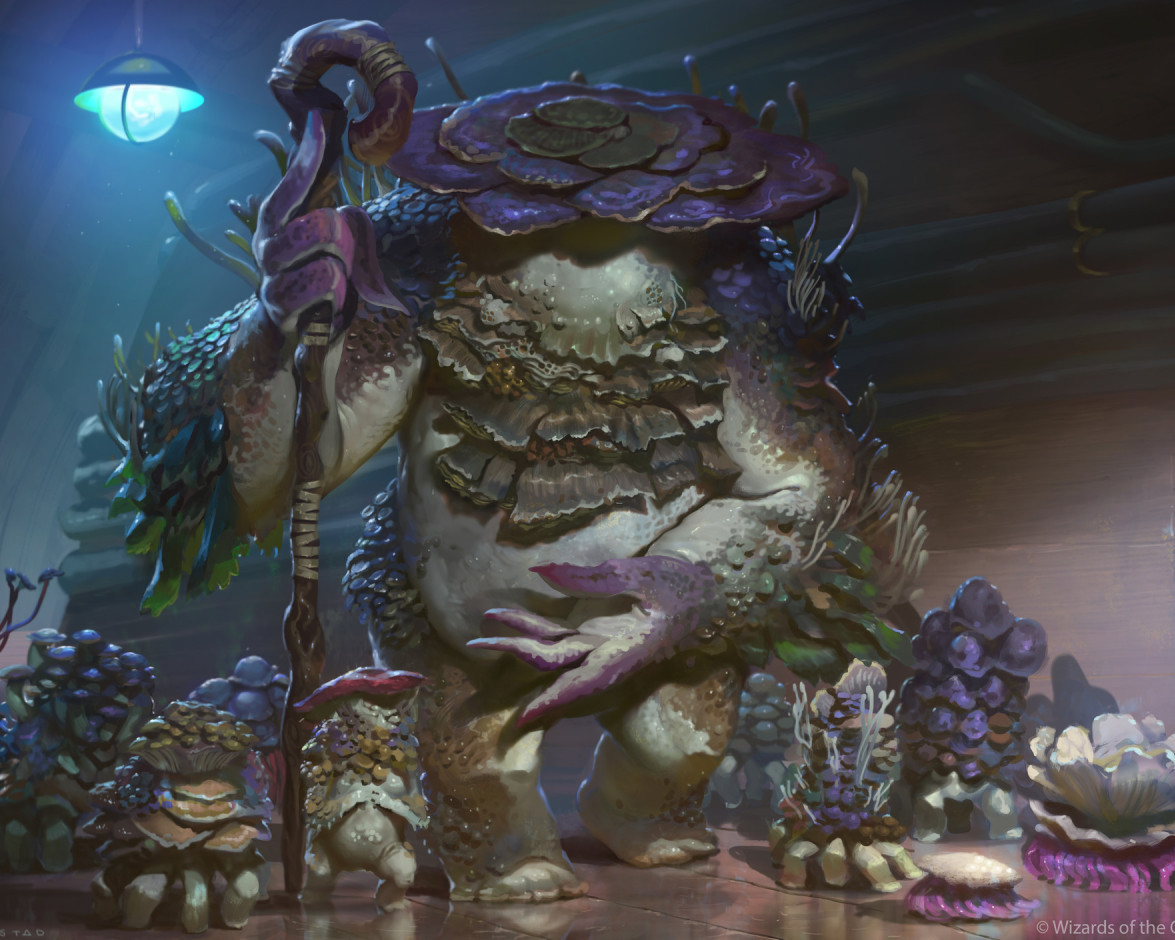
\includegraphics[width=0.98\textwidth]{03kins/img/16tsanek_sovereign.jpg}
    \end{DndTable}
\end{table*}

\subsubsection{Gannagian Tsanek}
Fungal kin that are members of the tribes in Drejeck which surround tekatsae.
Like their mold kin brothers, they have a very strong sense of community and devotion to their groups, the sovereigns and the tekatsae tree.
They are the spiritual leaders of the different groups, and focus on coordinating the tribes and communicating with the sovereigns.

\subparagraph{Ability Score Increase} You focused much of life in study, and your Wisdom score increases by 1.

\subparagraph{Drug-enhanced Spores} Your Rapport Spores' range is increased to 9 meters.
The spell save DC of all your spores is increased by 2.

\subparagraph{Euphoria Spores} Accustomed to fighting with the naenk warriors, you can release a specialized cloud of spores in a 6-meter-radius sphere centered on yourself.
Other creatures in the area must make a Constitution saving throw of a DC equal to 8 + your Constitution modifier or become poisoned for 1 minute.
A creature can repeat this saving throw at the end of each of its turns, ending the effect early on itself on a success.
When the effect ends, the creature gains one level of exhaustion.
You can produce these spores a number of times equal to your Constitution modifier (minimum of 1) per long rest.

\subsubsection{Na'anian Tsanek}
Sometimes, a tsanek will decide to abandon the tribe and break its link with the tekatsae tree.
These tsanek, unable to forgo their community lifestyles, tend to join or form fungus kin communities in the caverns of the world, sometimes spawning huge underground fungus cities.

\subparagraph{Ability Score Increase} Your meandering in hostile environments has granted you increased resilience, and your Constitution score is increased by 1.

\subparagraph{Sun Sickness} You become poisoned if you spend more than 1 minute in direct, unobstructed sunlight.
This conditions ends when you spend 1 minute in dim or dark conditions.

\subparagraph{Superior Darkvision} Accustomed to the darkness of the deepest of caverns, you have superior darkvision in dark and dim conditions.
You can see in dim light within 36 meters of you as if it were bright light, and in darkness as if it were dim light.

\subparagraph{Meld} When you take a short rest in the presence of one or more other tsaneks, you can meld with them.
After melding, you and all melding tsaneks regain all expended Hit Dice and gain the following benefits:
\begin{itemize}
    \item You have advantage on a saving throw you make in the next 24 hours.
    \item You can end one disease or condition affecting you, be it blinded, deafened, paralyzed, or poisoned.
\end{itemize}

\subparagraph{Communal Intellect} Your time spent melding with the others of your kin has granted you a deeper understanding of the world and yourself.
You are competent in the Insight and Religion skills, and you have advantage on Wisdom (survival) checks made to find your way in caverns.

\end{linenumbers}

\newpage

% !TEX root = ../main.tex
% TODO: GENERAL CHECKUP NEEDED

\section{Shelled Kin}
\begin{linenumbers}
\textit{I caught a big fish.}

\textit{Now I search for a good friend}

\textit{To share my lunch with.}

\hspace*{\fill} --- Tortle haiku.

The shelled kin are a species native to the outer lands.
Also known as tortles, they have gracefully adapted to their lives in Yuadrem, able to start a new life in the land ravaged by the schism, and it is very common to see the rustic tortle villages in the coasts of the beryl sea and many of the eastern shores of the continent.
% The shelled kin or tortles are a species native to the outer lands which, unlike umans, don't seem to be hunted by the strange creatures from this place, and remain unaffected by the forbidden lands.

What many tortles consider a simple life, others might call a life of adventure.
Tortles are born near sandy coastlines, but as soon as they're able to walk on two legs, they turn into nomad survivalists eager to explore the wilderness, experience its many wonders, put their skills to the test, and make new acquaintances.

\begin{figure}[!b]
    \centering
    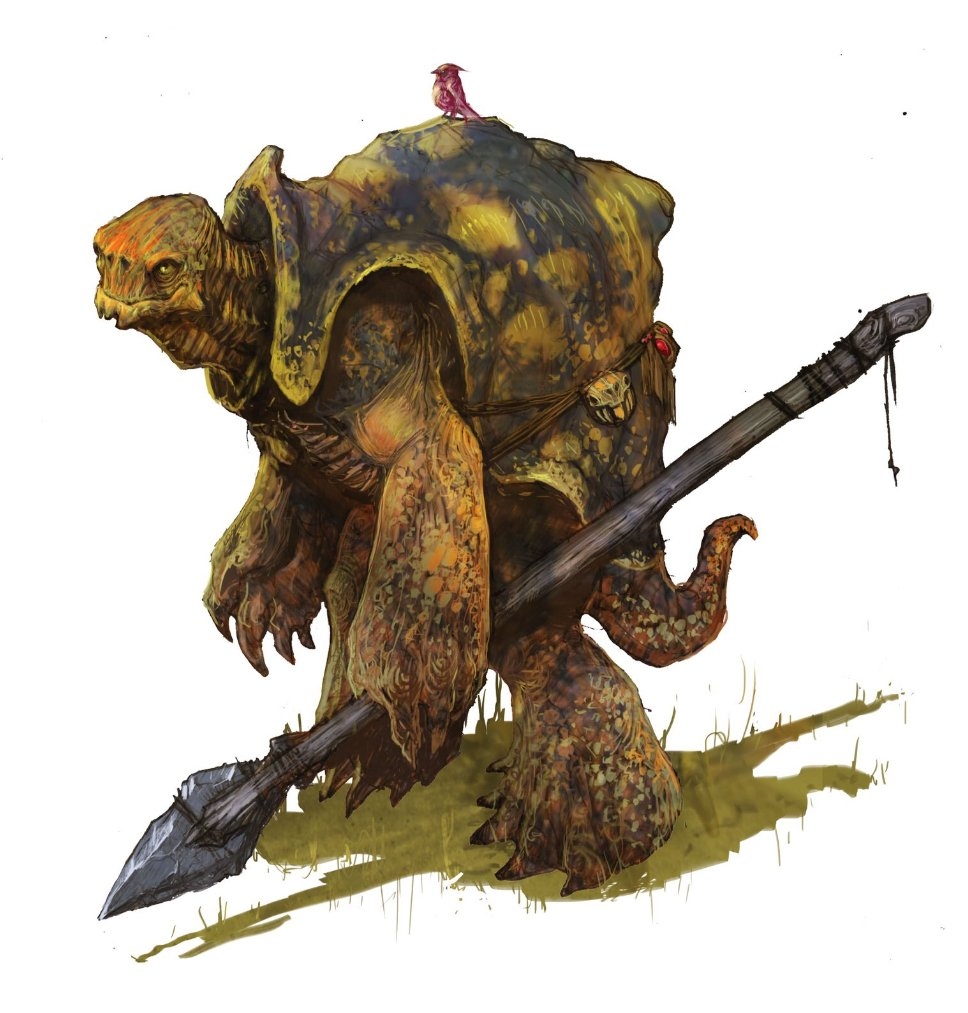
\includegraphics[width=0.48\textwidth]{03kins/img/17tortle_official.jpg}
\end{figure}

\subsection*{Life of a Tortle}
A tortle hatches from a thick-shelled egg and spends the first few weeks of its life crawling on all fours.
Its parents usually leave soon after its birth, but spend what little time they have telling stories to their offspring.
Within a year, the young tortle is abandoned and becomes an orphan, though not before it learns to speak and to survive on its own.

A young tortle and its siblings inherit whatever tools, weapons, and gifts their parents leave for them.
Each young tortle is expected to fend for itself.
It leaves the place of its birth and finds its own corner of the wilderness in which to hunt, catch fish, and get by.
With each passing year, a tortle hones its survival skills.
It forms friendships with its neighbors while also respecting their privacy.
At some point, a tortle feels an almost overwhelming urge to venture far away from home and see more of the world.
It gathers up its possessions and heads into the wilderness, returning months or years later with stories of its exploits and new skills.

Tortles are gendered creatures, and it is usual for them to seek out a mate and procreate when they return home from these travels.
Tortles lay their eggs (numbering as few as one or as many as a dozen) in a fortified compound enclosed by stone walls that are easily defensible.
If no such compound exists, they build one.
The parents spend the hatching time of their eggs guarding the compound and defending their offspring, and after they hatch they spend a year sharing their knowledge with the young ones.
The parents leave their children at this time, overburdened by their nomadic nature and confident that the older tortles of the village will care for them.
When the children are old enough to leave the compound, they pick up whatever weapons and tools their parents left behind and set out on their own.

\subsection*{Beliefs}
Tortles don't have a religion of their own, but they often worship the gods of other races.
It's not unusual for a tortle to hear stories or legends related to a god and choose to worship that deity.
Curious in nature, most tortles like to see how other creatures live and discover new customs and new ways of doing things.
Some tortles are also drawn to the many schools of thought, trying to learn from all of them instead of focusing on a single one.

Tortles believe that night and day watch over them and other creatures.
The moons are the eyes of night that watch over them in darkness, and the sun is the equally vigilant eye of day.
Tortles feel most at peace when these ``eyes'' are looking down on them.
They become more nervous and uneasy when no orb is visible in the sky.
Tortles tend to be most uncomfortable underground, where neither the sun nor the moons are visible to them.

Blessed are the days when many moons are visible in the sky at the same time.
Tortles often choose such days to leave their homes and begin a wilderness expedition, or perform some other task they know to be dangerous.

\subsection*{Inherent Mutualism}
Tortles have a special relationship to the anchelons.
Anchelons are colossal horned turtles that reside in Yuadrem's oceans, breeding fear among sailors and fishers alike.
They are generally fierce in nature but, while not sentient, they are oddly friendly toward tortles.
Anchelons lay their eggs in the beryl sea, and tortles allow thme to lay their eggs in their compounds.
It is not uncommon for baby anchelons to grow alongside tortles.
Anchelons in exchange protect the tortles' villages, and may even help tortles they encounter in the wilds.

\begin{table*}[b]%
    \begin{DndTable}[width=\linewidth]{X}
        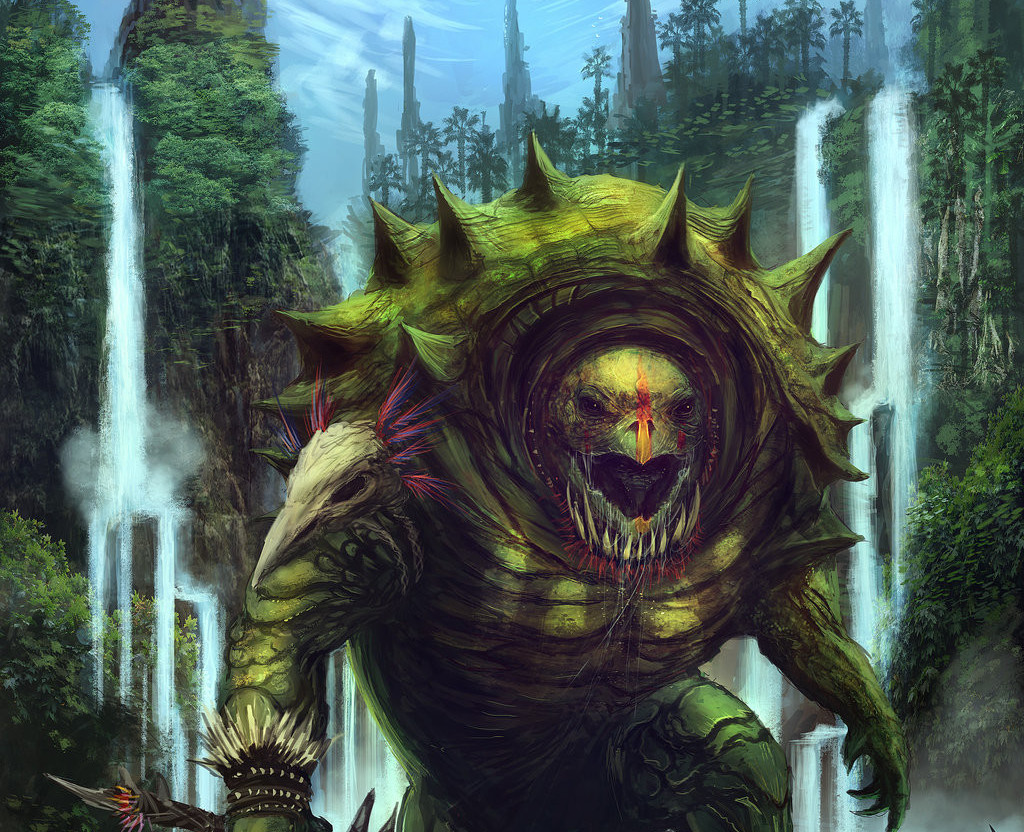
\includegraphics[width=0.98\textwidth]{03kins/img/17tortle_spiked.jpg}
    \end{DndTable}
\end{table*}

\subsection*{Adventurers at Heart}
Tortles have a saying: ``We wear our homes on our backs''.
The shells they carry around provide all the shelter they require.
Consequently, tortles don't feel the need to root themselves in one place for too long.
A tortle settlement is primarily used as a kind of moot, where tortles can socialize with one another, share useful information, and trade with strangers in the safety of greater numbers.
Tortles don't regard these settlements as places worth defending with their lives, and they will abandon a settlement when it no longer serves their needs.

Tortles embrace a simple view of the world.
It is a place of wonder, and tortles see beauty in the ordinary.
They live for the chance to hear a soft wind blowing through palm trees, to watch a frog croaking on a lily pad, or to stand in a crowded marketplace.

Tortles like to learn new skills.
They craft their own tools and weapons, and they are good at building structures and fortifications.
They marvel at the works of other kins, and can lose themselves for years in a city, studying its architectural wonders and learning skills they can put to use when building forts to contain their offspring.

Although they spend a considerable portion of their lives in isolation, tortles are social creatures that like to form meaningful friendships.
Being native to another world, they have no inbred animus toward any kin.
In fact, a tortle will often seek out friendships with non-tortles to learn new customs and new points of view.

% \begin{figure}[!htbp]
%     \centering
%     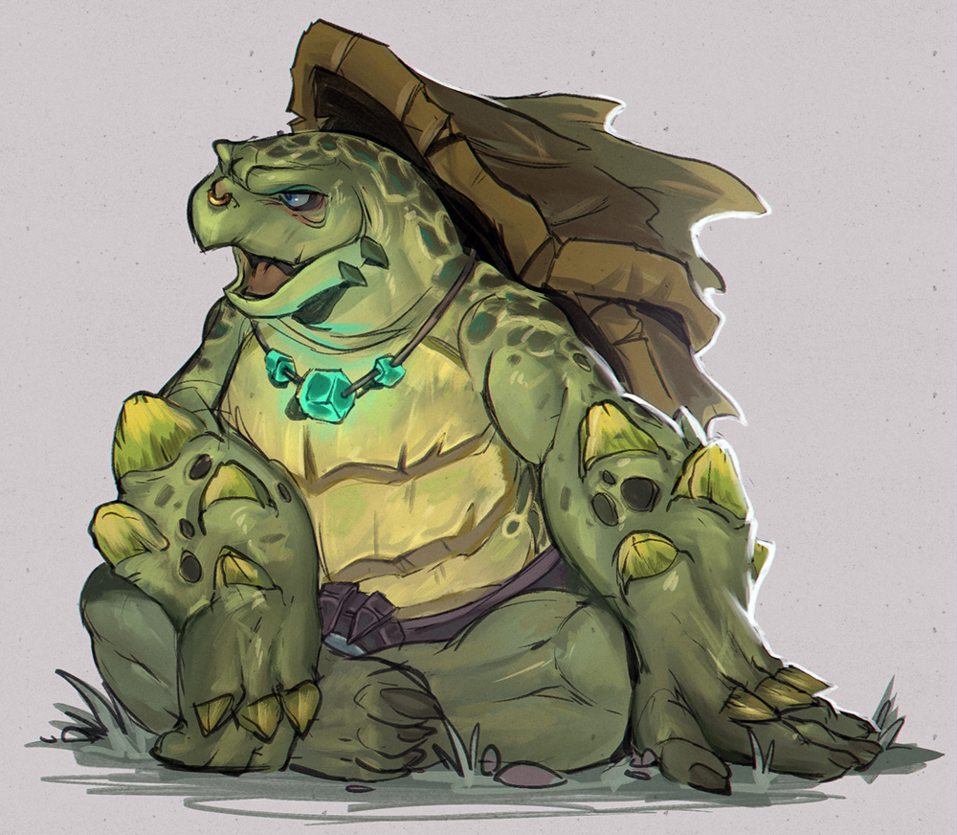
\includegraphics[width=0.48\textwidth]{03kins/img/tortle_chill.png}
% \end{figure}

\subsection*{Tortle Names}
Tortles prefer simple, non-gender-specific names that are usually no more than two syllables long.
If a tortle doesn't like its name for whatever reason, it can change it, and it might do this a dozen times in its life.

A tortle doesn't feel constrained by its name, which is designated only to refer to the tortle in contrast of its peers.
Tortles don't have surnames or family names.

\paragraph{Names}
Baka, Damu, Gar, Gura, Ini, Jappa, Kinlek, Krull, Lim, Lop, Nortle, Nulka, Olo, Ploqwat, Quee, Queg, Quott, Sunny, Tibor, Ubo, Uhok, Wabu, Xelbuk, Xopa, Yog

\subsection*{Traits}
Your tortle character gains traits that enable it to cope with the perils of a savage world.

\subparagraph{Ability Score Increase} Your Strength score increases by 2, and your Wisdom score increases by 1.

\subparagraph{Age} Young tortles crawl for a few weeks after birth before learning to walk on two legs.
They reach adulthood by the age of 15 and live an average of 500 years.

\subparagraph{Alignment} Tortles tend to lead orderly, ritualistic lives.
They develop customs and routines, becoming more set in their ways as they age.
Most follow a set of tenets that the kin brought with them from the outer lands, leading to lawfulness.
While most are good, a few can be selfish and greedy, but it's unusual for a tortle to shuck off order in favor of chaos.
Tortles tend towards the gold tide, always empathic and helping others.

\subparagraph{Size} Tortle adults stand 1.5 to 1.8 meters tall and average 230 kg.
Their shells account for roughly one-third of their weight.
Your size is Medium.

\subparagraph{Hold Breath} Tortles aren't natural swimmers, but they can remain underwater for some time before needing to come up for air.
You can hold your breath for up to 1 hour at a time.

\subparagraph{Natural Armor} Due to your shell and the shape of your body, you are ill-suited to wearing armor.
Your shell provides ample protection, however; it gives you a base AC of 17 (your Dexterity modifier doesn't affect this number).
You gain no benefit from wearing armor, but if you are using a shield, you can apply the shield's bonus as normal.

\subparagraph{Shell Defense} You can withdraw into your shell as an action.
Until you emerge, you gain a +4 bonus to AC, and you have advantage on Strength and Constitution saving throws.
While in your shell, you are prone, your speed is 0 and can't increase, you have disadvantage on Dexterity saving throws, you can't take reactions, and the only action you can take is to use an action to emerge from your shell.

% \subparagraph{Survival Instinct} Tortles have finely honed survival instincts.
% You gain competency in the Survival skill.

\subparagraph{Learned Tradition} You gain competency with either two weapons, two sets of artisan's tools, or one of each of your choice.
This ability comes from the time spent with your parents, and you feel a special connection with these types of items.

\subparagraph{Languages} You can speak the krehlo tongue and one additional language of your choice, but cannot write or read either.
The krehlo tongue doesn't have a written form, and the tortle tenets are passed on in oral tradition.

\end{linenumbers}

\newpage

% !TEX root = ../main.tex
% TODO: GENERAL CHECKUP NEEDED

\section{Poison Kin}
\begin{linenumbers}
\DndDropCapLine{T}{hey're a poison spilled down onto}
\textit{ our world, I tell ya'!
Grungs're bad.
They real bad!
They tell ya' their skin be the worst part o'em, but they don't know!
The spears mon.
It's the spears!}

\hspace*{\fill} --- Kleeck recounts her brief visit to Mabela.

Also known as grungs, the poison kin are aggressive creatures that look similar to dart frogs.
The species quickly settled into the chirping wilds and the areas surrounding the rainforest after their arrival during the schism.
They are fiercely territorial and see themselves as superior to most other creatures.

\subsection*{Class Structure}
Grung society is a caste system.
Each caste lays eggs in a separate hatching pool, and juvenile grungs join their caste upon emergence from their hatchery.
All grungs are a dull greenish gray when they are born, but each individual takes on the color of its caste as it grows to adulthood.
From lowest to highest caste, grungs are green, blue, purple, red, orange, and gold.

Green grungs are the tribe's warriors, hunters, and laborers, and blue grungs work as artisans and in other domestic roles.
Supervising and guiding both groups are the purple grungs, which serve as administrators and commanders.
Red grungs are the tribe's scholars and sorcerers.
They are superior to purple, blue, and green grungs and given proper respect even by the grungs of higher status.
Higher castes include orange grungs, which are elite warriors that have authority over all lesser grungs, and gold grungs, which hold the highest leadership positions.
A tribe's sovereign is always a gold grung.

A grung normally remains in its caste for life.
On rare occasions, an individual that distinguishes itself with great deeds can earn an invitation to join a higher caste.
A mixture of godsblood, seawater and poison is blessed by a red grung, and by drinking it the elevated grung changes color and is inducted into its new caste in the same way that a juvenile of the caste would be.
From then on, the grung and its progeny are members of the higher caste.

\subsection*{Poisonous Skin}
All grungs secrete a substance that is harmless to them but poisonous to other creatures.
A grung can also use this secretion as venom to coat its weapons.
Grungs are always on the lookout for creatures they can capture and enslave, and use slaves for all manner of menial tasks and hard labor.
Slaves are fed mildly poisoned food to keep them lethargic and compliant.
A creature afflicted in this way over a long period of time becomes a shell of its former self, and it seldom can be restored to normalcy.
Being amphibious, grungs require water to live; any grung that fails to immerse itself in water for at least 1 hour during a day becomes quite exhausted.

\subsection*{Whistle Stick}
All grungs are trained to use a musical instrument called the whistle-stick.
This is a hollow wooden tube with holes cut throughout, much like a flute.
Grungs play music with it for entertainment, but can also swing it about by a sturdy cord to create a sound recognizable by others of their kin, so they know each other's approximate location.
Additionally, any creature that can speak the krehlo language can use a whistle stick in this manner to communicate over distance.

\subsection*{Outcast or Voyager}
Since social advancement among grungs can only be achieved by a great deed, it is not unusual for a grung or a small group of them to travel around the coasts and rivers of Yuadrem.
They attempt to obtain renown by murdering an enemy of their civilization, or by bringing a rare artifact or important strategic information.

While a rare occurrence, sometimes an individual grung or even entire family-lines can grow disillusioned by the hardships of class advancements.
Some of them decide to escape from their cities, leading lives of their own as independent colonies or as members of the rare cities or towns willing to accept them.
Individuals from these groups are known to follow a life of adventure to help their communities or simply to satiate an internal need for excitement in the grung's heart.

\subsection*{Grung Names}
Grungs usually have simple, non-gender-specific names with a strong consonant joined by a syllable with a glottal stop, but members of higher castes prefer longer, more elaborate names to reflect their status.
Their names don't actually come from the krelho language, but are made based on what's easier to pronounce for the grung.
Grungs also wear their city of origin as surname.

\paragraph{Names}
B'ang, B'leep, B'lip, B'loop, Bl'eg, Bl'myeek, Bl'ngiip, Ch'eg, Ch'rol, D'aht, D'khan, F'huu, Fl'aak, Fl'uup, G'lahp, Gh'rol, K'eet, K'riig, K'ung, R'ang, R'loo.

\paragraph{Surnames} Bakagar, Bomqueeg, Gor, Int, Joppank, Kangaru, Limlim, Mabela, Obu, Om, Ploqlek, Queequio, Quott'nem, Uhok'moa, Wewat, Xilkoko, Zipqueg.

\begin{figure}[!t]
    \centering
    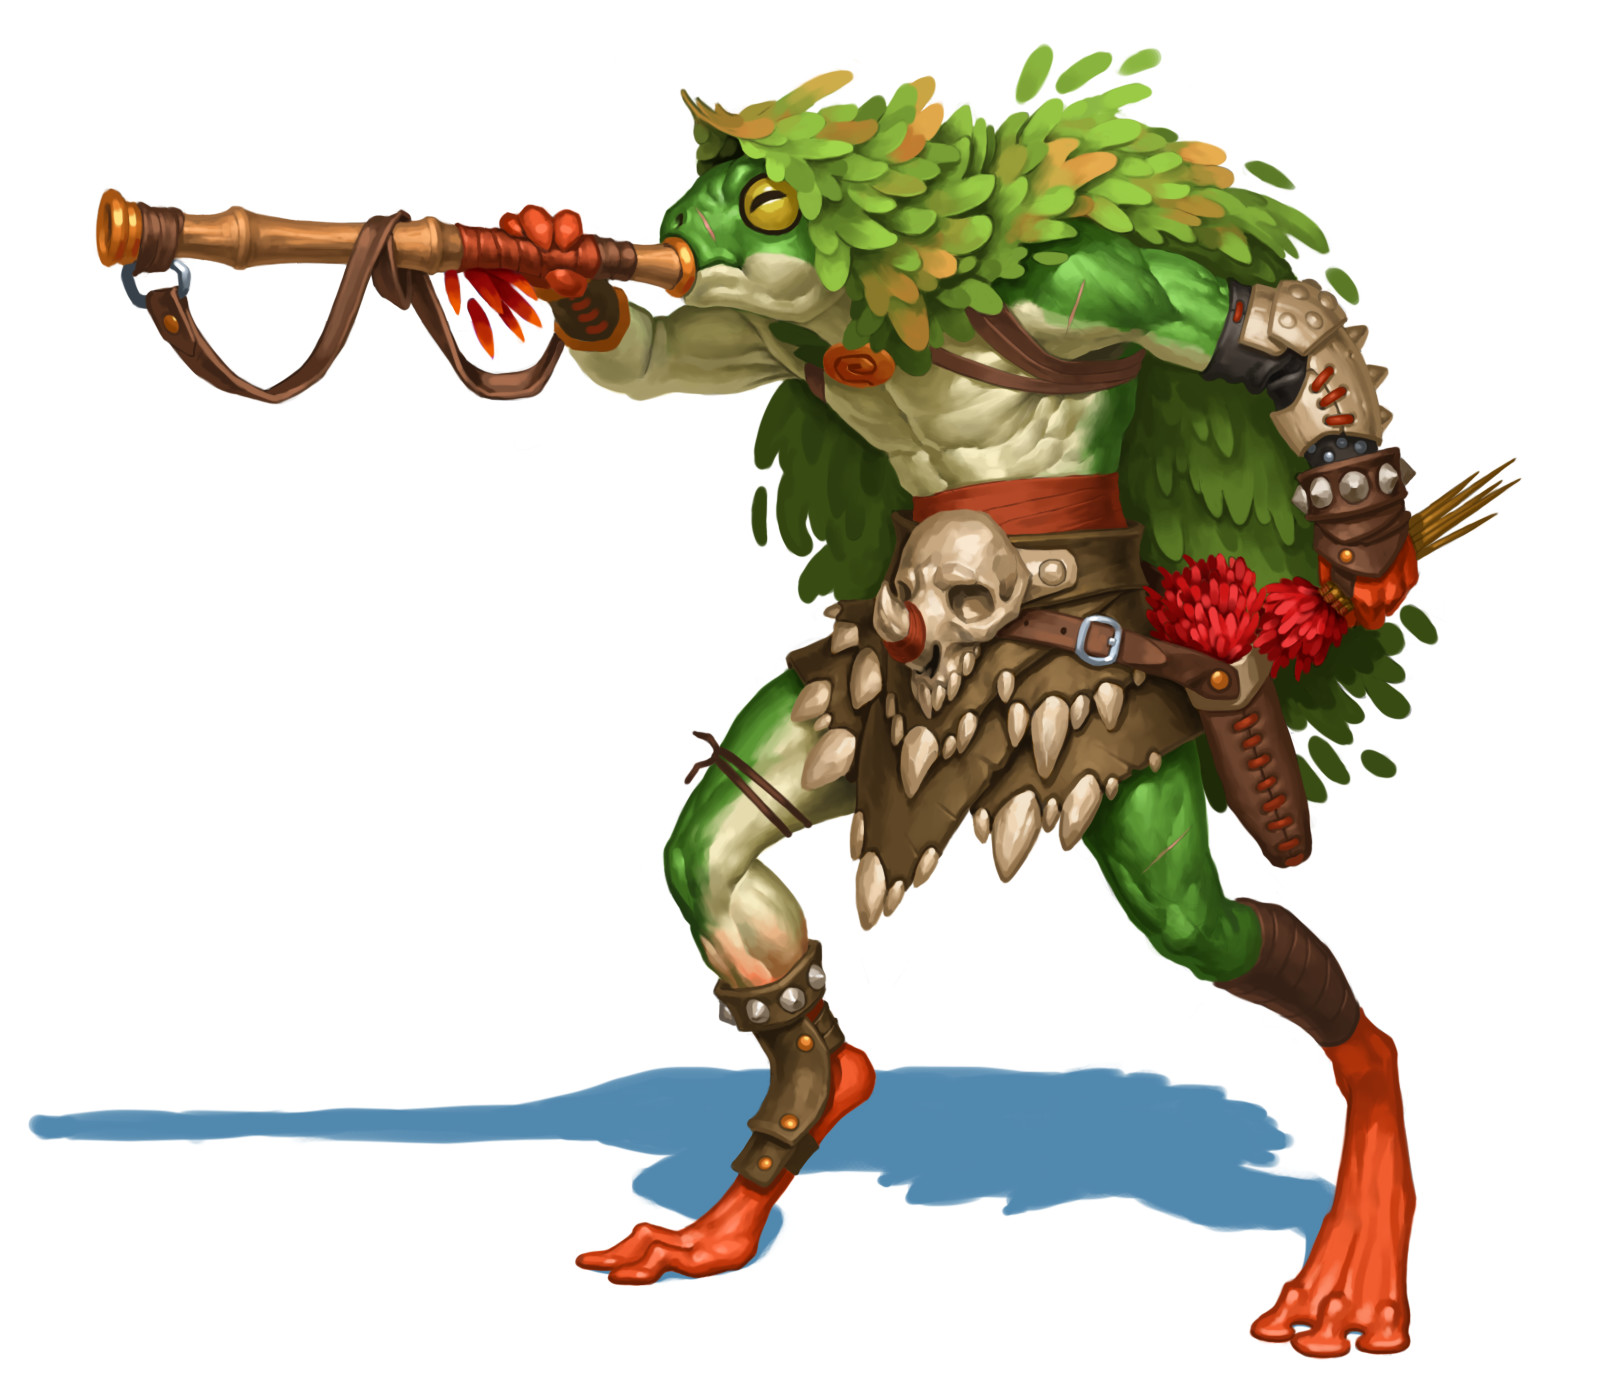
\includegraphics[width=0.48\textwidth]{03kins/img/18grung_blowgun.jpg}
\end{figure}

\subsection*{Traits}
Your grung character has an assortment of inborn abilities, part and parcel of grung nature:

\subparagraph{Ability Score Increase} Your Dexterity score increases by 2, and your Constitution score increases by 1.

\subparagraph{Age} Grung reach adulthood in a single year, and can live for up to 80 years.

\subparagraph{Alignment} % Most grungs are lawful, having been raised in a strict caste system.
% Grung society is in constant search of power, and most individual grung look forward to very rare social advancement.
Grungs are in constant search of power, and move along the silver tide.

\subparagraph{Size} Grungs stand between 75 and 105 cm tall and average about 20 kg.
Your size is small.

\subparagraph{Speed} Your base walking speed is 7.5 meters, and you have a climbing speed of 7.5 meters.

% \subparagraph{Arboreal Alertness} You are competent in the Perception skill.

\subparagraph{Amphibious} You can breathe both air and water.

\subparagraph{Poison Resistance} You are resistant to poison damage.

\subparagraph{Poisonous Skin} Any creature that grapples you or otherwise comes into direct contact with your skin must succeed on a Constitution saving throw of DC 8 + your Consitution modifier, becoming poisoned for 1 minute on a fail.
A poisoned creature no longer in direct contact with you can repeat the saving throw at the end of each of its turns, ending the effect on a success.

You can also apply this poison to a slashing or piercing weapon as an action. % though when you hit the poison reacts differently.
The target must succeed on the same saving throw or take 2d4 poison damage.
A grung succeeds on these saving throws automatically.

A creature poisoned by a grung suffers an additional effect that varies depending on the grung's skin color.
This effect lasts for one turn and can only be used once per short rest.

\paragraph{Green Toxins} The poisoned creature can't move except to climb or make standing jumps.
If the creature is flying, it can't take any actions or reactions unless it lands.

\paragraph{Blue Toxins} The poisoned creature must shout loudly or otherwise make a loud noise at the start and end of its turns.

\paragraph{Purple Toxins} The poisoned creature feels a desperate need to soak itself in liquid or mud.
It can't take actions or move except to do so or to reach a body of liquid or mud, unless no such body can be found in a 18 meter radius.

\paragraph{Red Toxins} The poisoned creature feels extreme hunger and must use its action to eat something or to move towards a source of food, unless no source of food can be found in a 18 meter radius.

\paragraph{Orange Toxins} The poisoned creature becomes frightened of its allies.

% \paragraph{Gold Toxins} The poisoned creature is charmed and permanently learns how to speak basic krehlo.

\subparagraph{Standing Leap} Your long jump is up to 7.5 meters and your high jump is up to 4.5 meters, with or without a running start.

% \subparagraph{Grung Weapon Training} Due to combat training, you are proficient with spears, blowguns, and nets.

\subparagraph{Inflatable Cheek Pouches} Due to your frog-like anatomy, you are able to shoot darts at incredible speed.
You are competent with blowguns, and with it you can shoot darts to a range of 15/30 meters.
Additionally, you can apply your poison to the darts as part of your attack with them.

% \subparagraph{Water Dependency} If you fail to immerse yourself in water for at least 1 hour during a day, you suffer one level of exhaustion at the end of that day.
% You can only recover from this exhaustion by immersing yourself in water for at least 1 hour.

\subparagraph{Languages} You can speak the krehlo tongue and one additional language of your choice, but cannot write or read either.

\begin{figure}[!b]
    \centering
    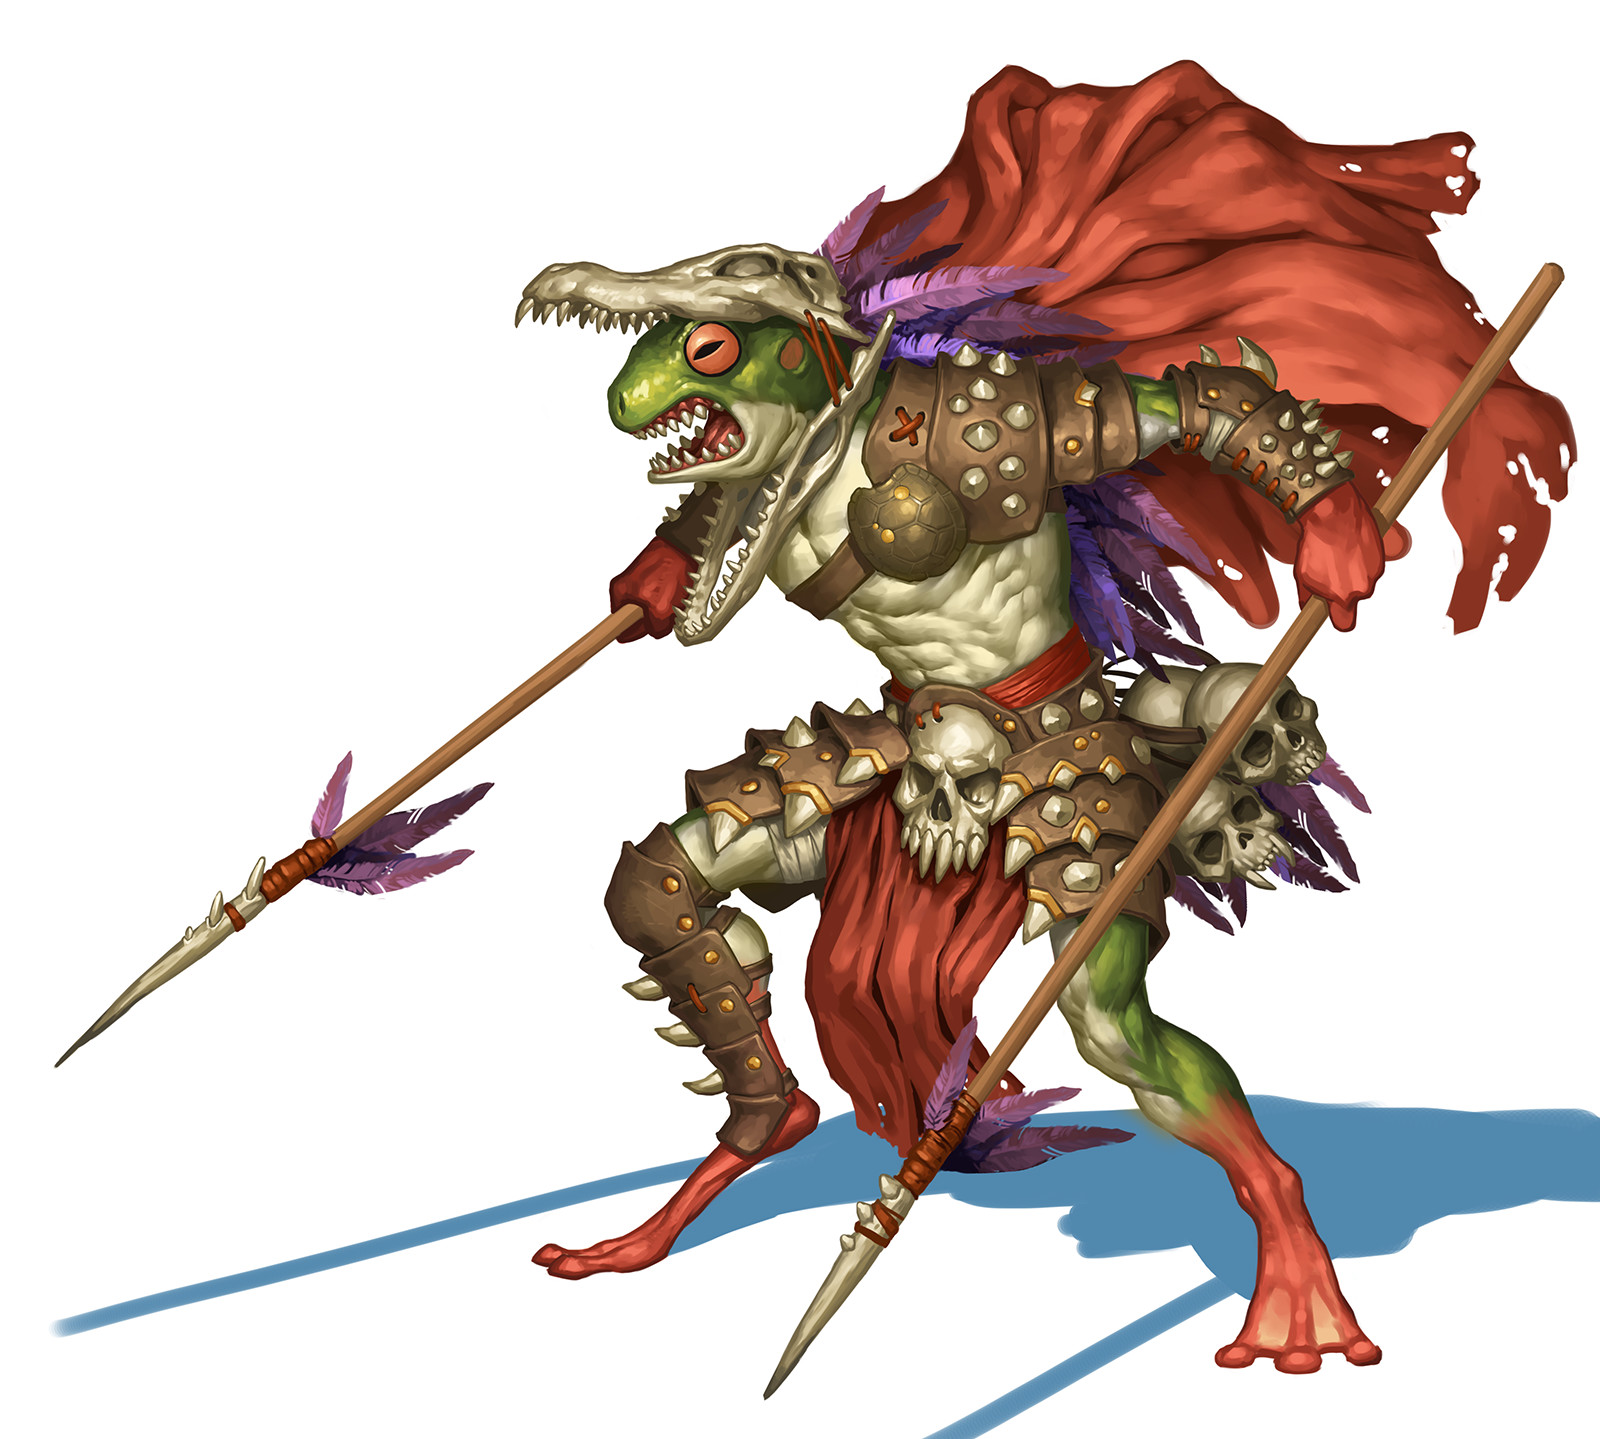
\includegraphics[width=0.48\textwidth]{03kins/img/18grung_warrior.jpg}
\end{figure}
\end{linenumbers}

\newpage

% !TEX root = ../main.tex
\begin{linenumbers}

\section{Nomad Kin}
\DndDropCapLine{O}{utsiders, the lot of them. Dragged}
\textit{into our world by an unnatural pull, ever unable to find stable footing.
No matter how much they beg and cry, do not allow them into your home.
Touched by a strange flame, whose brightness attracts equally as strange beasts into your door, into your hearth.
Get rid of them before they share their misfortune with you.}

\hspace*{\fill} --- Abneh, renowned nimrod.

Brought into this world with the Schism, the nomad kin are a strange race from the outer lands.
Also known as umans, they have almost hairless bodies, and are similar in appearance to apes.

For an unknown reason, umans attract all kinds of predators from these lands.
Additionally, their blood has similar properties to the tall ones', and is used in many rituals.
Because of these reasons, umans are dispersed all around the world, and are nomadic in nature.

\subsection*{A Broad Spectrum}
Hunted by all kinds of kin and creatures, the nomad kin are forced to perpetually migrate and adapt to different environments, making them more physically diverse than the common kins.

There is no typical uman, with an individual standing from 1.5 meters to a little over 1.8 meters tall, and weighing from 60 to 125 kgs.
Acclimating to even the most extreme environments, a uman's skin shades to any color from the darkest brown to the lightest hues.
They also grow long hair in their scalps and faces, sporting a great variety of colors and thickness.
Nomads reach adulthood at around 14, and rarely live a single century.

Umans are a gendered kin, and usually have one child at a time.
Families consist of a father, a mother, and their kid or children, but it is not uncommon for other members of the nomadic groups to care for parentless children.

\subsection*{Accursed Coldblood}
Known as coldblood due to its cerulean tint, Umans' blood has special properties, and is very useful for spellcasters.
It retains a sort of energy, and can be used as a source of spells.
Umans know this, and regularly prepare blood vials for trade and to strengthen troupes' wizards.

Umans pay dearly for this special blood, as it acts as a beacon for the predators from the outer lands, the coldblood beasts.
These creatures hunt umans, and many of the kin are banned from villages for safety concerns.

Spellcasters seek coldblood, and many try to attain it by any means available.
Naturally, the murder of umans for their blood is illegal in most nations, but some carry the custom on nevertheless.
The nimrods are a cult that specializes in gathering coldblood via any means available, and are commonly contracted by wizards and warlocks to attain the product.

\subsection*{Adaptable and Durable}
Hunted by both beast and kin, umans have trouble trusting others and don't normally settle in communities of other kins.
They live in troupes exclusive to their kin, where usually all members have some familiar relationship.
Troupes travel together and care for each other, assigning specific roles to each member based on their skills.

Far from vulnerable, most troupes are fierce and resilient, hardened by centuries of being preyed upon.
Groups keep track of how they are treated by different cities and towns, and only do commerce where they are accepted.

While uncommon, some uman communities have managed to settle in one place.
These communities keep their locations secret, communicating it only to other umans via traveller's cant, a set of writings and symbols they brought from the outer lands.

\subsection*{Life in Escapade}
For a uman, a life of adventure is not a romantic desire but rather a fact of mundane life.
Used to the hardships of survival, a uman is especially capable of fending off threats and surpassing hardships.

It is very common to see lone uman adventurers, either as exiles or in a quest for their troupe.
Whatever the motive, they naturally excel at voyages, and are a great fit on any adventuring party.

\subsection*{Uman Names}
Umans most commonly wear names from other cultures.
Even in the outer lands, umans were known to have a great variety of names depending on each specific culture.
Those who desire to conserve their roots choose old names from their history and legends to give their children.

\paragraph{Common Names}
(Male) Anton, Aseir, Diero, Dorn, Evendur, Grim, Haseid, Ivor, Khemed, Kosef, Marcon, Morn, Pavel, Pieron, Rimardo, Romero, Salazar, Sergor, Umbero, Zasheir;
(female) Atala, Arveene, Balama, Ceidil, Chessail, Dona, Faila, Jasmal, Luisa, Lureene, Marta, Quara, Rowan, Seipora, Selise, Shandri, Vonda;
(surnames) Agosto, Amblecrown, Astorio, Basha, Buckman, Calabra, Domine, Evenwood, Falone, Greycastle, Khalid, Kulenov, Marivaldi, Marsk, Nemetsk, Pashar, Pisacar, Ramondo, Rein, Starag.

\paragraph{Frostburn Names}
(Male) Ander, Blath, Bran, Frath, Geth, Lander, Luth, Malcer, Stor, Taman, Urth;
(female) Amafrey, Betha, Cefrey, Kethra, Mara, Olga, Silifrey, Westra;
(surnames) Brightwood, Helder, Hornraven, Lackman, Stormwind, Windrivver.

\paragraph{Boggart Names}
(Male) Aoth, Bareris, Ehput-Ki, Kethoth, Mumed, Ramas, So-Kehur, Thazar-De, Urhur;
(female) Arizima, Chathi, Nephis, Nulara, Murithi, Sefris, Thola, Umara, Zolis;
(surnames) Ankhalab, Anskuld, Fezim, Hahpet, Nathandem, Sepret, Uuthrakt.

\begin{figure}[!b]
    \centering
    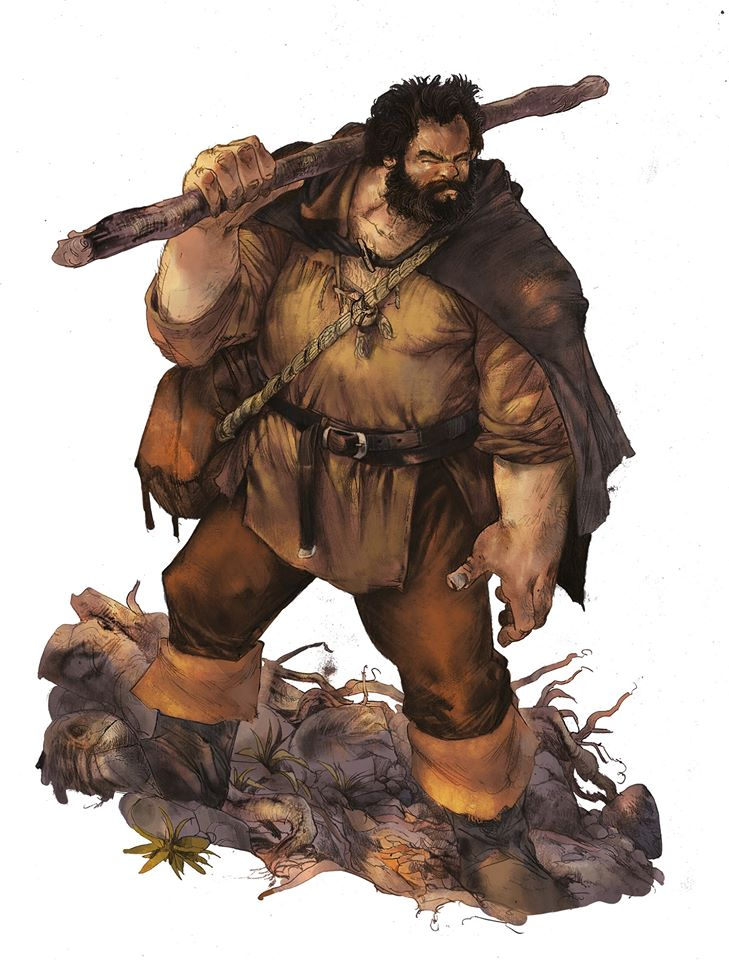
\includegraphics[width=0.48\textwidth]{03kins/img/19uman_monk.jpg}
\end{figure}

\subsection*{Traits}
The nomad kin is known for their survival and adaptability, and your uman character receives the following traits:

\subparagraph{Ability Score Increase} Two different ability scores of your choice are increased by 1.

\subparagraph{Age} Umans reach adulthood in their late teens and live less than a century, if they manage to survive that long.

\subparagraph{Alignment} Umans tend to no particular alignment, but they do have a penchant for community and justice, and tend to the indigo tide.

\subparagraph{Size} Umans vary widely in height and build, from barely 1.5 meters to well over 1.8 meters tall.
Regardless of your position in that range, your size is Medium.

\subparagraph{Speed} Your base walking speed is 9 meters.

\subparagraph{Languages} You can speak, read, and write the nomad tongue, and an additional language of your choice.
You can also read and write the traveller's cant, a set of writings and symbols created by your kin to help and communicate with each other.

\subparagraph{Learned Durability} You are competent in the Survival skill.

\subparagraph{Relentless Endurance} When you are reduced to 0 hit points but not killed outright, you can drop to 1 hit points instead.
You can't use this feature again until you finish a short rest.

\begin{figure}[!t]
    \centering
    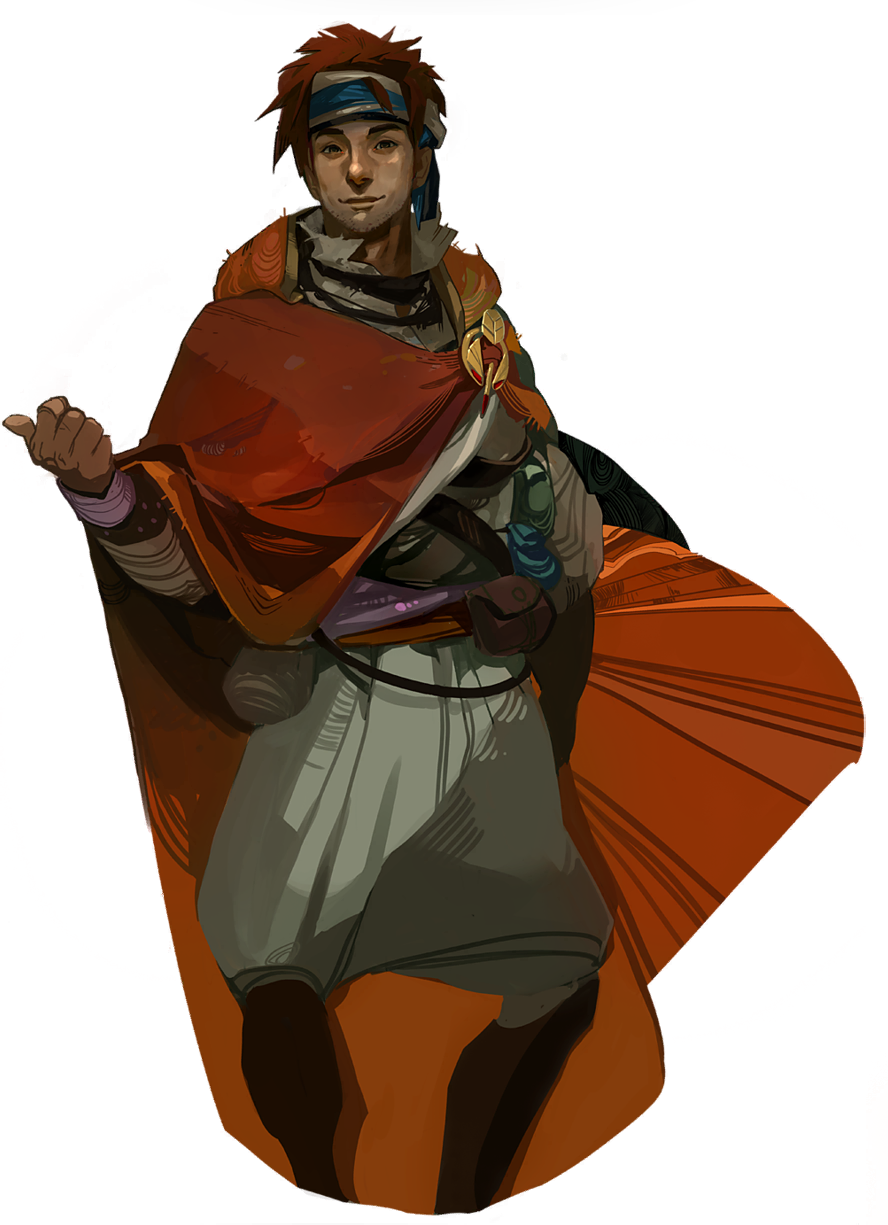
\includegraphics[width=0.48\textwidth]{03kins/img/19uman_nomad.png}
\end{figure}

\subsubsection{Common Nomad}
While umans are known to be extremely adaptable to extreme habitats, most don't stay at one place for enough time to acquire this specialty and remain, for lack of a better word, common.
In stark contrast with their name, each of these umans is unique and as such your features are specially dynamic.

\subparagraph{Languages} You can read, write and speak one additional language of your choice.

\subparagraph{Skills} You gain competence in one skill of your choice.

\subparagraph{Trained} You gain competence with one simple or martial weapon of your choice.

\subparagraph{Handy} You gain competence with a set of artisan's tools of your choice.

% \subparagraph{Feat} You gain one feat of your choice.

\subsubsection{Frostburn Nomad}
With skins ranging from pale blue to light purple, and hair shades from the lightest of white to deep brown colors, the Frostburn are a kin that comes from a troupe of umans that managed to survive in the lands beyond the wall of ice and stone, and beyond the reach of most coldblood beasts and nimrods.
%These umans tend to dress with the bones and furs of the creatures they hunt, using their inventiveness to craft clothing to intimidate and scare rather than protect against cold, since their thick skins already manage this task effortlessly.

\subparagraph{Ability Score Increase} Your Constitution score is increased by 1.

% \subparagraph{Menacing} You are competent in the Intimidation skill.

\subparagraph{Born Hunter} You are competent with clubs, daggers, spears, and barbed spears.

\subparagraph{Thick Skin} %You are naturally acclimated to cold environments and don't need sources of heat to survive in all but the most extreme cold.
You are resistant to cold damage.%, and remain unaffected by cold environments.

\subparagraph{Ice Shell} As two actions, you can grow a thick layer of ice around your body to protect you.
You gain resistance to piercing and slashing damage and vulnerability to bludgeoning damage for a number of turns equal to your Constitution modifier (Minimum of 1).
Additionally, any creature that attacks you with a melee attack during this time suffers 1d4 piercing damage.
You can use this trait once per short rest.

\subsubsection{Boggart}
Boggarts are umans that live in the swamps and marshes of Yuadrem.
Boggarts are generally tall, slim, and amber-skinned, with eyes of hazel or brown.
Their hair ranges from black to dark brown, but most shave off all their hair.
These umans are craftier than the average, and are known to prepare complex traps and mechanisms to protect their communities or alert them of imminent danger.

\subparagraph{Ability Score Increase} Your Wisdom score is increased by 1.

\subparagraph{Bog Swimmer} Boggart tactics usually include a good dose of swimming through less than cooperative waters.
You have a swimming speed of 9 meters.

\subparagraph{Swamp Life} You have advantage on saving throws against poison and diseases, and you have resistance against poison damage.

\subparagraph{Stealthy Hunter} You are competent with blowguns, nets, and bolas.
% You also are proficient with a Poisoner's kit.

\subsubsection{Cursed Kin}
It is said that the umans who remain in the place of their arrival start showing their true form.
While the accuracy of this statement remains untested, it is true that those who stay in the forbidden lands do show strange changes to their appearance.
Large, black horns grow on their heads, their skin and eyes turn into a very pale shade, and their bodies grow.
While most cursed kin do act more menacing and violent than the average uman, it is likely that this is a side effect of their harsh homeland more than a natural development in their minds.

\subparagraph{Size} Unlike most nomad kin, you stand between 2.1 and 2.4 meters tall and weight between 140 and 170 kg.
Your size is medium.

\subparagraph{Ability Score Increase} Your Strength score is increased by 1.

% \subparagraph{Natural Athlete} You have proficiency in the Athletics skill.

\subparagraph{Abyssal Resistance} You have resistance to fire damage.

\subparagraph{Unholy Fortitude} Your hit point maximum increases by an amount equal to your number of hit dice.

\subparagraph{Ram} Your horns are a natural weapon, which you may use use to make unarmed strikes.
If you hit with them, you deal bludgeoning damage equal to 1d4 + your Strength modifier, instead of the damage normal for an unarmed strike.

\subparagraph{Powerful Build} You count as one size larger when determining your carrying capacity and the weight you can push, drag or lift.

\begin{figure}[!b]
    \centering
    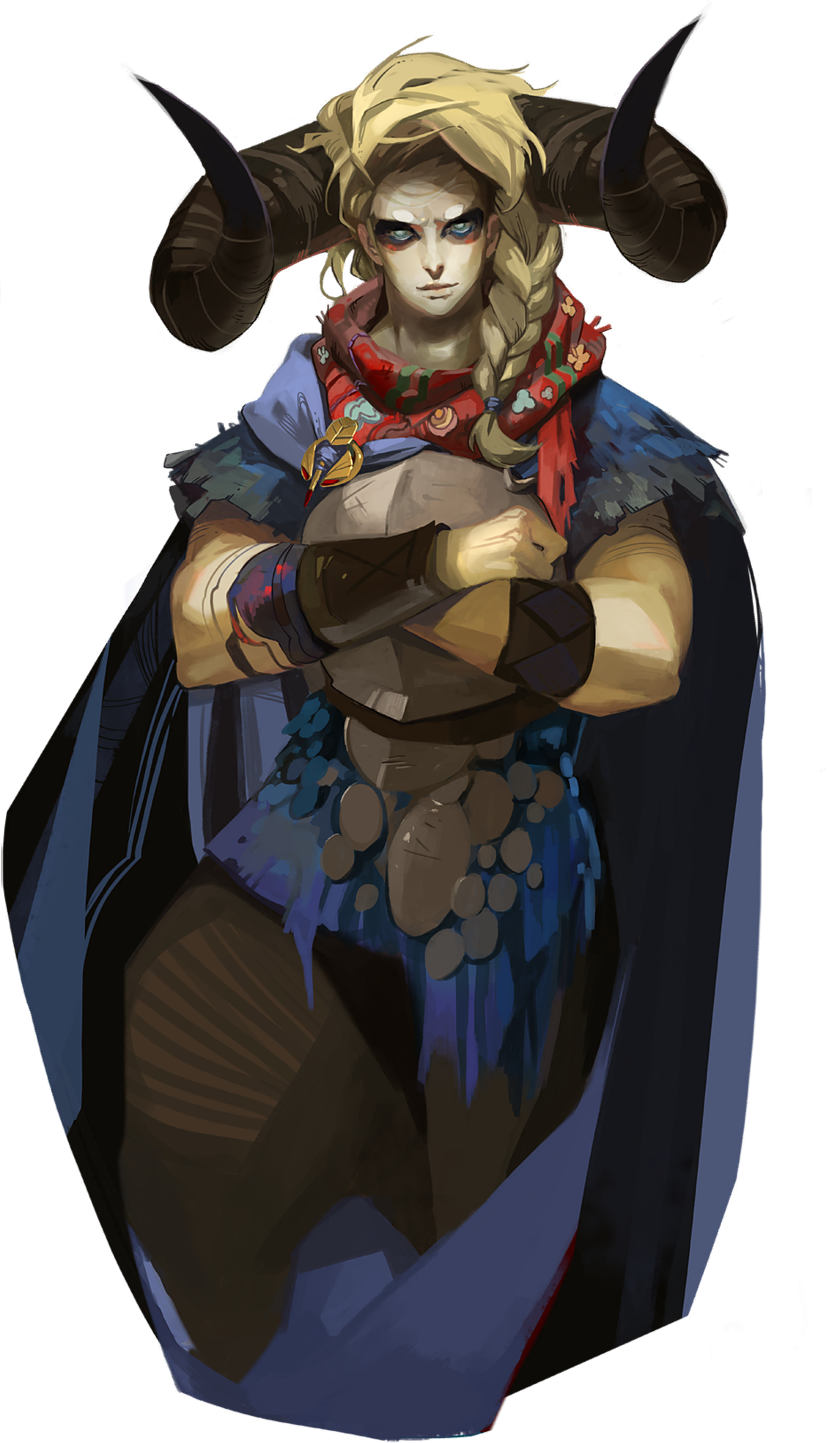
\includegraphics[width=0.48\textwidth]{03kins/img/19uman_cursed.png}
\end{figure}
\end{linenumbers}

% !TEX root = ../main.tex
\begin{linenumbers}

\section{Storm Kin}
\DndDropCapLine{A}{sk anyone anywhere and they will give}
\textit{you a list of the things and people they lost to the ash storm.
That blasted cloud covered the entirety of the continent, leaving none unscarred.}

\hspace*{\fill} --- Iitus the scholar, "Of War and Thunder".

As the schism progressed, when the spire started spewing forth smoke and lava into the world, an immense ash storm gathered around the volcano, discharging lightning into anyone foolish enough to approach it.
As the years passed, the storm slowly subsided, leaving behind a strange race of being composed of ash, smoke, and lightning.
These being were named the zaloths, or storm kin, who adapted surprisingly well to the many kins of Yuadrem, and quickly found their new place in the world.

\subsection*{Ethereal Appearance}
The zaloths are tempests given physical shape, and their form reflects this.
They are composed of ash smoke, with strange forces shaping them into humanoid form.
Born from storm, they are in constant turmoil, and lightning sparks and cackles incessantly inside their bodies.

It is social norm for zaloths to clothe themselves in linen wrappings to cover their bodies, and it is not unusual for them to wear clothes or armor over these wrappings.
When they were formed, they also took the qualar of the unfortunate sentient creatures that were atop or near the spire, thus retaining their sentience.

Zaloths are not known to age or reproduce, and as such it's hard to tell if they'll be able to survive too long as a species.
They are thus extremely appreciative of their chance to experience life on Yuadrem, and are commonly known to be existentialists, looking to maximize their experiences in number and intensity.

When a zaloth suffers a mortal wound it does not die in a traditional sense, but the matter composing its body coalesces into a zaloth quintessent, a small cloud of ash.
This cloud does not retain its sentience, but it is somewhat able to keep its memories and experiences, and eventually merges into the atmosphere, becoming part of Yuadrem in a sense.

\subsection*{Distributed and Nomadic}
While a small group of zaloths established themselves in the city of Jan'krug at the top of the spire, the vast majority of the storm kin immediately started roaming the world alone or in small groups, looking for experiences.
Due to this, it is very rare to encounter an established zaloth community or zaloths living permanently in a city or town.
Nowadays, they are found wondering the land in caravans, circuses or as lone adventurers, eternally seeking new experiences.

When a wandering zaloth group meets another, it is common for them to celebrate this encounter by throwing a party in commemoration of their common heritage.
During this event, the members of the different groups conduct a ritual known to them as the mingling, where they allow their bodies to fuse, and thus share with each other their memories and experiences.

\subsection*{Presence in the World}
Due to their rarity, the other kins generally treat them with wonder and even admiration.
Many schools of thought regard the zaloths as sages due to the wisdom obtained in their nomadic ways, and their unique viewpoint on life and the world is appreciated by any who seek knowledge.

This however does not mean that all zaloths describe themselves as savant.
On the contrary, some of them give in to their inherent chaotic nature and become agents of turmoil, seeking paramount experiences via extreme means.
While their methods are frowned upon by more orthodox zaloths, they are far from being a pariah; they engage in mingling as commonly as any other zaloth.

\subsection*{Life of Adventure}
Due to the existentialist nature of the zaloths, a life of adventure is the most natural lifestyle that comes to them.
However, most zaloths are far from reckless, and while they can find dangers in their travels, they are careful to avoid mortal danger.
To the storm kin, any zaloth's death is a tragedy, and they prioritize the life of any of their kin over that of all other creatures.

A traveling zaloth will try all sorts of activities, independent of their nature and intensity.
Ever seeking new experiences, it is equally likely to encounter a zaloth engaging in quiet appreciation of nature, martial combat against formidable enemies, or joining in on other species' religious rituals.
Or even all of these activities on the same day.

\subsection*{Zaloth Names}
Due to the special conditions to their coming into the world, zaloths are born without names.
A zaloth usually chooses a name for itself after years, decades or even centuries of travel, and while it is nameless it is referred to using a feat or special characteristic that defines it.
The names that a zaloth chooses are commonly taken from other cultures or carefully designed by it.

\paragraph{Names} Basks-in-the-Sun, City-Swimmer, Dreams-of-Sleep, Dusk-Skin, Far-From-Water, Forest-Child, Has-no-Regrets, Head-in-Clouds, Iron-Fists, Mumbles-when-Speaks, Sees-All-Colors, Six-Coins, Somber-Mind, Sleeps-with-Open-eyes, Stands-in-Shallows, Swift-Legs, Takes-in-Light.

\begin{figure}[!t]
    \centering
    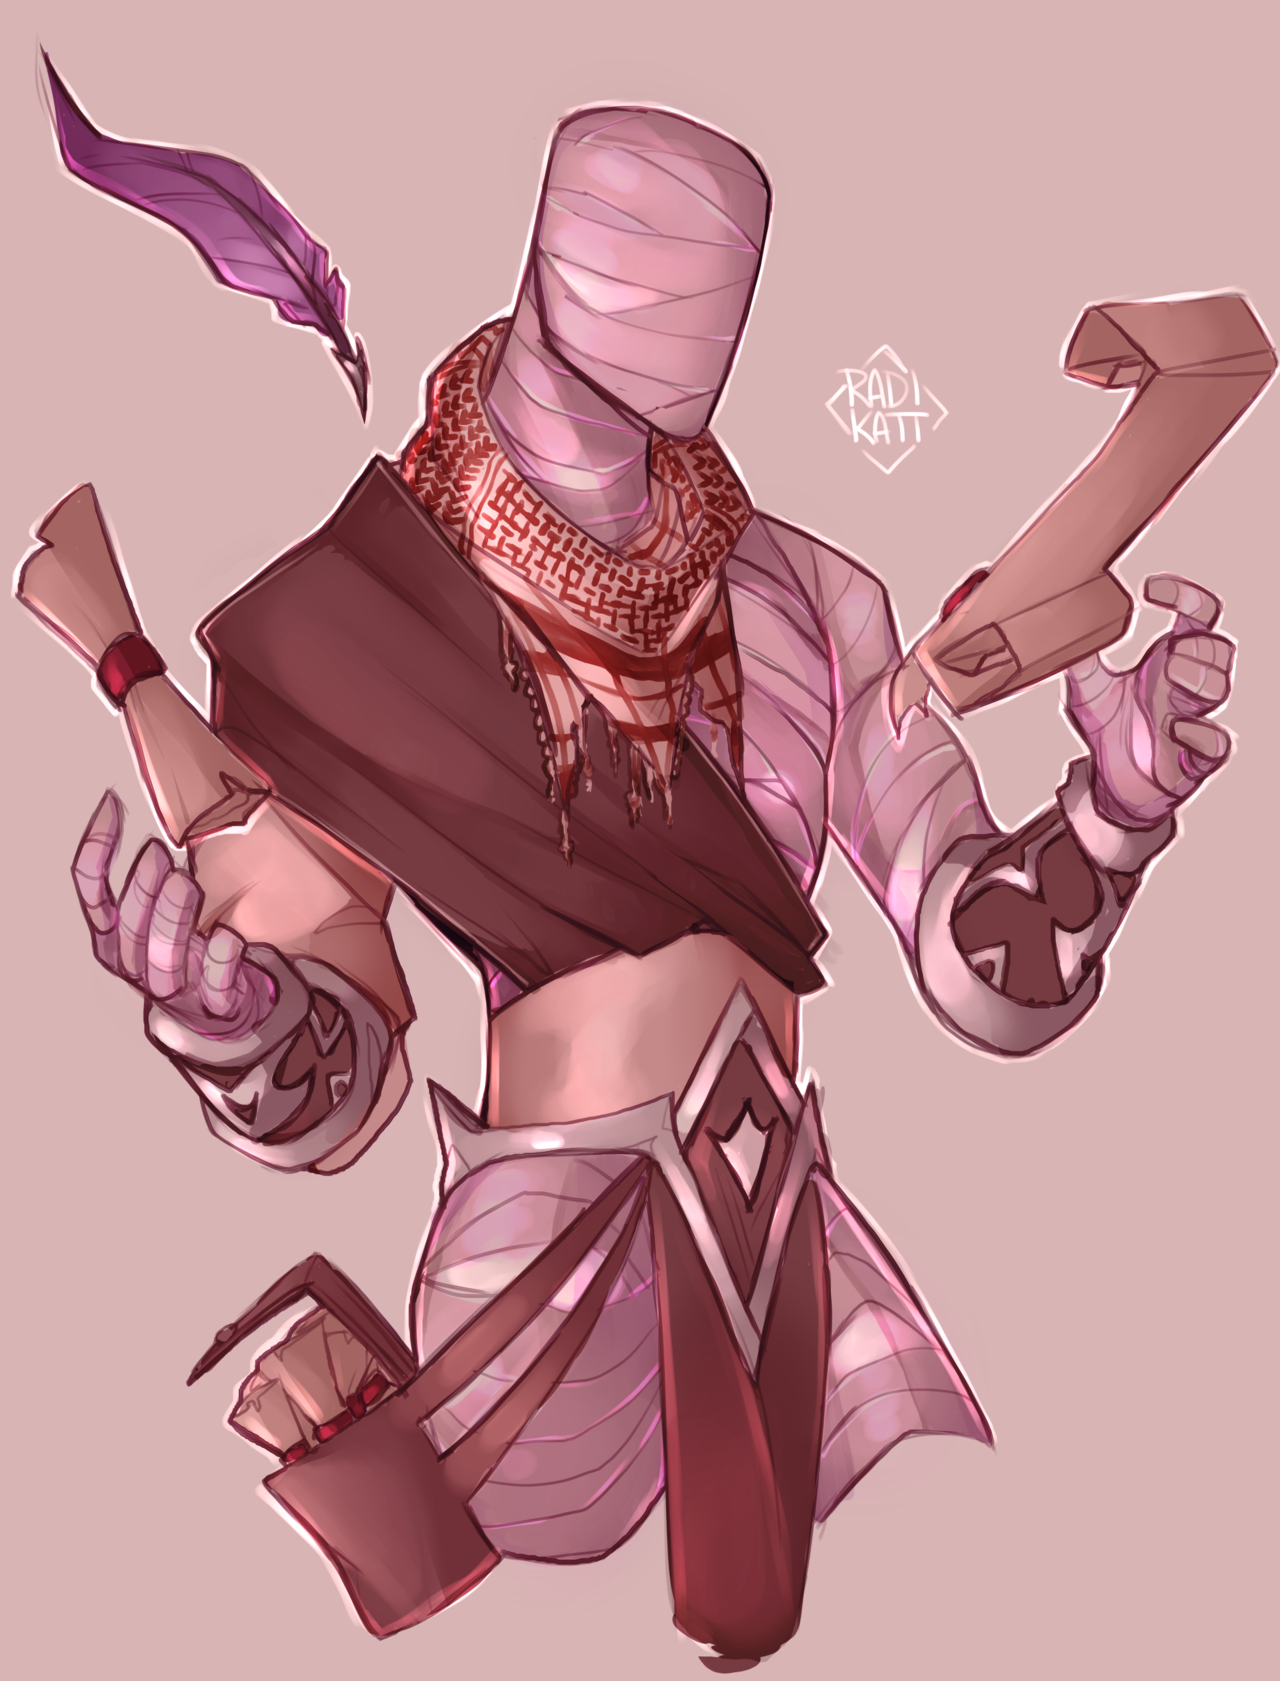
\includegraphics[width=0.48\textwidth]{03kins/img/20zaloth_scholar.png}
\end{figure}

\subsection*{Traits}
Your zaloth character has an assortment of traits related to its unique nature and nomadic lifestyle.

\subparagraph{Ability Score Increase} Your Charisma score increases by 1, and your Intelligence score increases by 1.

\subparagraph{Age} Born from an ash storm, a zaloth is thrust into adulthood, retaining some of the memories of the tall one from which it acquired its qualar as a blurry image.
Zaloths are not known to die from natural causes, and all of them are about 673 years old.

\subparagraph{Alignment} Most zaloth tend toward chaos, with little regard for the affairs of civilizations.
Due to their curious nature and lifestyle, zaloths move with the red tide.

\subparagraph{Size} Zaloths stand between 1.5 and 1.8 meters, and are practically weightless due to their unique composition.

\subparagraph{Speed} Your base walking speed is 9 meters.

\subparagraph{Dual Nature} You are both humanoid and elemental.
You can be affected by an effect if it works on either of these two creature types.

\subparagraph{Incorporeal} You are immune to poison damage, and cannot be affected by poison or disease.
Additionally, you don't need to eat or drink.

% \subparagraph{Hover} Instead of walking, your can choose to hover up to 1 feet over the ground.
% You can still be thrown into the ground if you are knocked prone, but you only need 5 feet of movement to stand up and don't provoke attacks of opportunity when you do so.

\subparagraph{Radiant} You give off dim light in a 3-meter radius and have disadvantage on Dexterity (Stealth) checks.
You cannot block this light with any clothing or armor.

\subparagraph{Telepathic} You can speak telepathically to any creature you can see within 9 meters of you.
Your telepathic utterances are in a language you know, and the creature understands you only if it knows that language.
Your communication doesn't give the creature the ability to respond to you telepathically.

\subparagraph{Silent Speaker} You can ignore the verbal components of spells.

\subparagraph{Languages} You can understand, read and write two languages of your choice, but you are unable to speak.
You can understand a very limited vocabulary of jantherlin, but your vocabulary consists of only individual words without context.

\subsubsection{Gale Zaloth}
Different zaloths have a stronger tendency towards different elements of the ash storm from which they were born.
Gale zaloths are attuned to the shifting, violent winds of the storm, and they reflect this with their erratic movements and shifting conversation subjects.
% A constant breeze can be felt around them, a grim reminder from the ash clouds.

\subparagraph{Ability Score Improvement} Your Dexterity score increases by 1.

\subparagraph{Stormbound} Wherever you go, you carry some of the storm with you.
A light breeze can be permanently felt in a 3-meter radius around you, moving in a random direction every turn.
The wind of this breeze displaces all smoke, gases, and very light objects inside its radius.
You can choose to end or restart this effect as a free action.

\subparagraph{Potent Quintessent} When you drop to 0 hit points, your desire to live manifests as a strong shockwave, sending any creature standing near you flying.
All creatures that stands in a 3-meter radius around you must succeed on a DC of 12 + your Constitution modifier Strength saving throw.
On a fail, a creature takes 1d6 force damage, is pushed 12 meters, and is knocked prone.
On success, a creature only takes half the damage, and isn't pushed or knocked prone.
You can use this ability once per short rest.

\subparagraph{Wind Given Form} You know the gust cantrip.
Once you gain your 3rd hit die, you can cast the feather fall spell.
Once you gain your 5th hit die, you can cast the dust devil spell as a 2nd level spell, requiring no material components.
Charisma is your spellcasting ability for these spells, and you can use each only once per short rest.

\subsubsection{Thunder Zaloth}
Thunder zaloths are attuned to the fleeting, fierce lightning.
They reflect this relation with their quick movements and sparking personalities.

\subparagraph{Ability Score Improvement} Your Charisma score increases by 1.

\subparagraph{Instant Step} You can expend your movement and a bonus action to transport instantly to a location up to your movement speed away that you can see.
Any creature standing in the straight line between the two positions must succeed on a DC 8 + your Constitution modifier Dexterity saving throw, taking 1d8 lightning damage on a failure.
You can do this a number of times equal to your Charisma modifier (Minimum of 1), and regain all expended uses when you complete a short rest.

\subparagraph{Elemental Resistance} You have resistance to lightning damage.

\subparagraph{Electricity Given Form} You know the shocking grasp cantrip.
Once you gain your 3rd hit die, you can cast the thunderwave spell as a 2nd level spell.
Once you gain your 5th hit die, you can cast the shatter spell as a 2nd level spell.
Charisma is your spellcasting ability for these spells, and you can use them only once per short rest.

\subsubsection{Ash Zaloth}
Ash zaloths are attuned to the destructive force of the spire, given form in the ash storm.
They embody the violence of the storm, and have affinity towards inflicting and receiving pain.

\subparagraph{Ability Score Improvement} Your Strength score increases by 1.

\subparagraph{Storm Conduit} The chaos of combat stirs your inner storm.
Once per round, you can deal an extra 1d4 fire damage to one creature you hit with an unarmed strike or an attack made with a metal weapon.
At 11th level, this damage increases to 2d4.
You can do this a number of times equal to your Charisma modifier (Minimum of 1), and you regain all expended uses when you complete a short rest.

\subparagraph{Elemental Resistance} You have resistance to fire damage.

\subparagraph{Flame Given Form} You know the produce flame cantrip.
Once you gain your 3rd hit die, you can cast the burning hands spell as a 2nd level spell.
Once you gain your 5th hit die, you can cast the Aganazzar's scorcher spell as a 2nd level spell.
Charisma is your spellcasting ability for these spells, and you can cast them once per short rest.

\subsubsection{Hail Zaloth}
Rarest of their species, the hail zaloths are the youngest of the zaloth, embodying the freezing hail into which the ash storm eventually decanted.
While still existentialist, they approach their curiosity in a calmer fashion, preferring the stillness of nature to the rowdiness of civilized society.

\subparagraph{Ability Score Improvement} You Wisdom score increases by 1.

\subparagraph{Cryogenic Stillness} You can choose to temporarily freeze your entire body, granting you extreme resilience.
As an action or reaction, you can instantly freeze, granting you immunity to slashing, piercing, and bludgeoning damage, apart from resistance to acid, force, lightning, necrotic, and thunder damage.
You also gain vulnerability to fire damage.
You are also affected by the slow spell for the duration of this trait without the possibility to roll saving throws.
You can maintain this effect for a number of turns equal to your Charisma modifier (minimum of 1), and must finish a short rest in order to use this trait again.

\subparagraph{Elemental Resistance} You have resistance to cold damage.

\subparagraph{Ice Given Form} You know the frostbite cantrip.
Once you gain your 3rd hit die, you can cast the ice knife spell as a 2nd level spell.
Once you gain your 5th hit die, you can cast the icy surface spell as a 2nd level spell.
Charisma is your spellcasting ability for these spells, and you can use them only once per short rest.

\begin{figure}[!b]
    \centering
    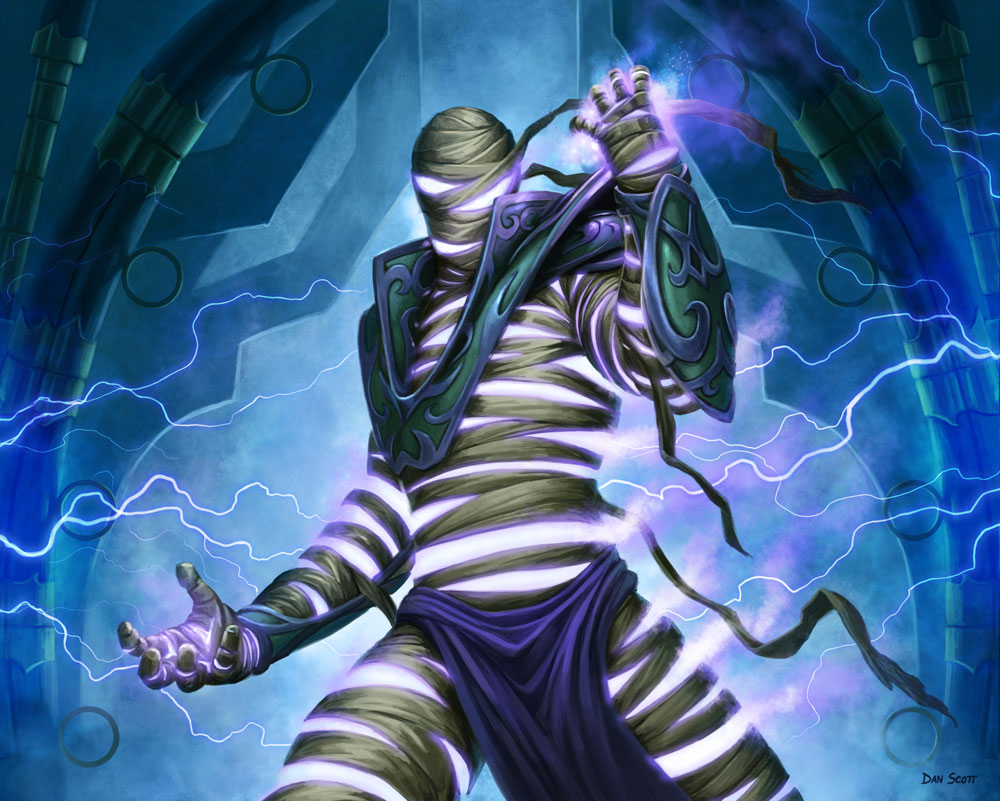
\includegraphics[width=0.48\textwidth]{03kins/img/20zaloth_thunder.jpg}
\end{figure}

\end{linenumbers}

\newpage

% !TEX root = ../main.tex
\begin{linenumbers}

\section{Retainer Kin}
\DndDropCapLine{T}{hey are the last kin made by our}
\textit{creators, and as such are related to us gats, irds, and oths.
It is our duty to provide them the nourishing that our shared parents denied them.
They are, after all, our younger siblings.}

\hspace*{\fill} --- Kosmael, founder of the church of Jismuah.

After the schism, as the storm that covered the tall kin's tiding dispersed, many dark secrets were revealed.
Among these sins, the existence of the quies, or retainer kin, was of special note.
The retainer kin is a fully sentient species which, unlike the other created by the tall kin, was forced into servitude, unable to comprehend what it is to roam free or even the existence of a world outside of Jan'krug.

At some point after the tall kin secluded themselves in their mountaintop city, they decided to create this slave race to focus solely on their studies and rituals.
The quies, not understanding what freedom is, remained immersed in their tasks for centuries, continuing even after the tall ones vanished.
They continued in this meaningless loop until gat expeditioners found them, still locked into servitude to their dead masters, and showed them a life unbound by chains.

\subsection*{Designed with a Purpose}
Such as gats, irds, oths, and marsets, the quies were created by the tall kin.
Unlike them, the quies were formed from a blend of organic and inorganic materials.
Their bodies are made from a blend of flesh and wood, with root-like cords infused with strange fluids serving as muscles, wrapped around a framework of bone and flesh.

Armored plates form a protective outer shell and reinforce joints.
Quies' faces are simply a collection of holes located where sensory organs would normally be, but each has a custom made qualar mask integrated into this outer shell.
These masks usually contain very intricate detail, and seem to be made with an almost ardent passion.

\subsection*{Functionalist at Heart}
The quies were built to serve.
For the first centuries of their existence, the retainer kin had a clearly defined function and were encouraged to focus purely on that role.
While they now might have freedom, many still struggle both to find a place in the world and to relate to the creatures of it.

The typical quies show little emotion.
Many of them embrace a concrete purpose-such as protecting allies, completing a contract, or exploring a land-and embrace this task as they once did.
However, there are quies who delight in exploring their feelings, their freedom, and their relationships with others.
The race was first welcome to Yuadrem by the church of Jismuah, and many embraced faith and mysticism, seeking higher purpose and deeper meaning.

\subsection*{Life of Subservience}
The quies are the sentient beings that spent the most time living alongside the tall kin, and as such they are highly sought after by scholars studying them.
While a quies can describe in great detail the daily life of a tall one, their subservient nature inhibited their curiosity.
Not one quies is known that can recall the rituals performed by the tall kin, and most can't even tell anything about their masters other done the tasks they performed for them.

Like the zaloths, the quies are unable to reproduce by any mean, which is probably by design.
This, combined with the fact that their creators have almost completely disappeared from Yuadrem, makes their chances of survival as a species look very grim.
This is countered however by the fact that, as their creators, quies don't seem to age at all.

\subsection*{New Beginnings}
After leaving Jan'krug, the retainer kin had a very hard time adapting to the world.
Some dedicate themselves to continuing their skill under a new patron, failing to leave behind their lives as servants.
Others managed to learn independence, but could not abandon their craft, and became renowned artisans or merchants, being compared by many even to gat artisans.

The quies that managed to completely break free from their bindings are regarded as special by the other members of their species, and they are met with both reverence and jealousy.
These quies usually become adventurers, where they can blend their newfound curiosity with their armored bodies.
Some take the plight of their kin into their hearts, and spend their lives trying to find the last remaining tall ones, aiming to learn how to create more of their own.

\subsection*{Quies Names}
As far as is known, no tall one ever gave a name to a quies.
Most of the retainer kin simply refer to themselves by their job, or by a name given to them by others.
However, the quies that manage to escape their shackles and take a life of wandering are very appreciative of being given the freedom to pick their own names.
Once chosen, a quies will guard their name with great jealousy, only sharing it with whom they trust the most.

\paragraph{Names} Ba, Bal, Dreth, Eth, Feather, Fish, Gakn, Green, I, Jan, Loth, Risz, Seed, Sekru, Stand, Swim, Tis, Tlekeloo, Tlos, When, Yu, Zash.

\begin{figure}[!t]
    \centering
    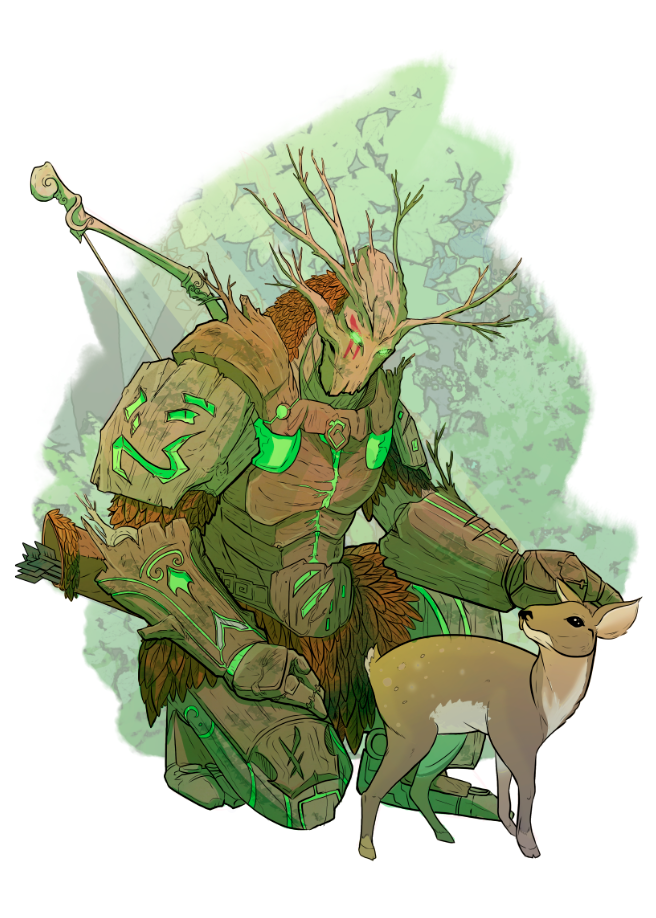
\includegraphics[width=0.48\textwidth]{03kins/img/21quies_druid.png}
\end{figure}

\subsection*{Traits}
Designed for efficiency, your quies character has the following traits:

\subparagraph{Ability Score Increase} Your Constitution and Strength scores increase by 1.

\subparagraph{Age} Every quies is somewhere between 673 and 890 years old, but their memories before the schism are vague and unreliable.
Since they've shown no sign of deterioration over time, quies are assumed to be impervious to aging.

\subparagraph{Alignment} Most quies take comfort in order and discipline, tending toward law and neutrality, but some have chosen a new morality based on the experiences of their independent life.
They came as a blank slate, and do not tend to any particular tide as a species.

\subparagraph{Size} Quies are of formidable size, standing between 1.8 and 2.25 meters tall.
Your build is determined by your subrace.
Your size is medium.

\subparagraph{Speed} Your base walking speed is 9 meters.

\subparagraph{Dual Nature} Due to your manufactured nature, you are both humanoid and construct.
You can be affected by an effect if it works on either of these two creature types.

\subparagraph{Quies Resilience} You were created with fortitude in mind.
You have advantage on saving throws against being poisoned, and you have resistance to poison damage.

\subparagraph{Integrated Protection} Your body has built-in defensive layers, which can be enhanced with armor:
\end{linenumbers}
\begin{itemize}
    \item You gain a passive +1 to Armor Class.
    \item You can only don armor with which you have proficiency.
    To don armor, you must incorporate it into your body as part of a short rest, during which you remain in contact with the armor.
    To doff armor, you must spend 1 hour removing it.
    \item While you live, your armor can't be removed from your body against your will.
\end{itemize}
\begin{linenumbers}

\subparagraph{Mountain Built} You are impervious to all effects related to altitude, including cold and lack of oxygen.

\subsubsection{Quies Operative}
You were designed with a certain specialized function in mind.
You might be a carpenter, a cartographer, or an entertainer, to name a few possibilities.

Operatives are the most common of the quies, yet each is of unique design.
Your build is dependent on the task you were designed for, and you can be as light as 70 kg to as heavy as 150 kg.

\subparagraph{Ability Score Increase} Any ability score of your choice increases by 1.

\subparagraph{Integrated Tool} You are competent with one set of artisan's tools or one instrument of your choice.
This tool or instrument is integrated into your body, and is related to what was your purpose when you lived in Jan'krug.
You must have your hands free to use this integrated tool.

\subparagraph{Specialized Design} You are competent with one skill of your choice.

\subsubsection{Juggernaut}
While many ets were more than capable of dealing with heavy lifting, they designed this branch of quies for fulfilling these tasks in conditions less ideal for them, or simply to work in cooperation with them.
Juggernauts have a large frame and powerful build, and can weigh up to 230 kg.
% While these quies were not specifically designed to fight, they usually prove more than capable of melee combat.

\subparagraph{Ability Score Increase} Your Strength score increases by 1.

\subparagraph{Hard Fists} Your arms and fists are lined with obsidian, a specially hard stone from the higher parts of the spire.
When you hit with an unarmed strike, you can deal 1d4 + your Strength modifier bludgeoning damage, instead of the normal damage for an unarmed strike.

\subparagraph{Powerful Build} You count as one size larger when determining your carrying capacity and the weight you can push, drag, or lift.

\begin{table*}[b]%
    \begin{DndTable}[width=\linewidth]{X}
        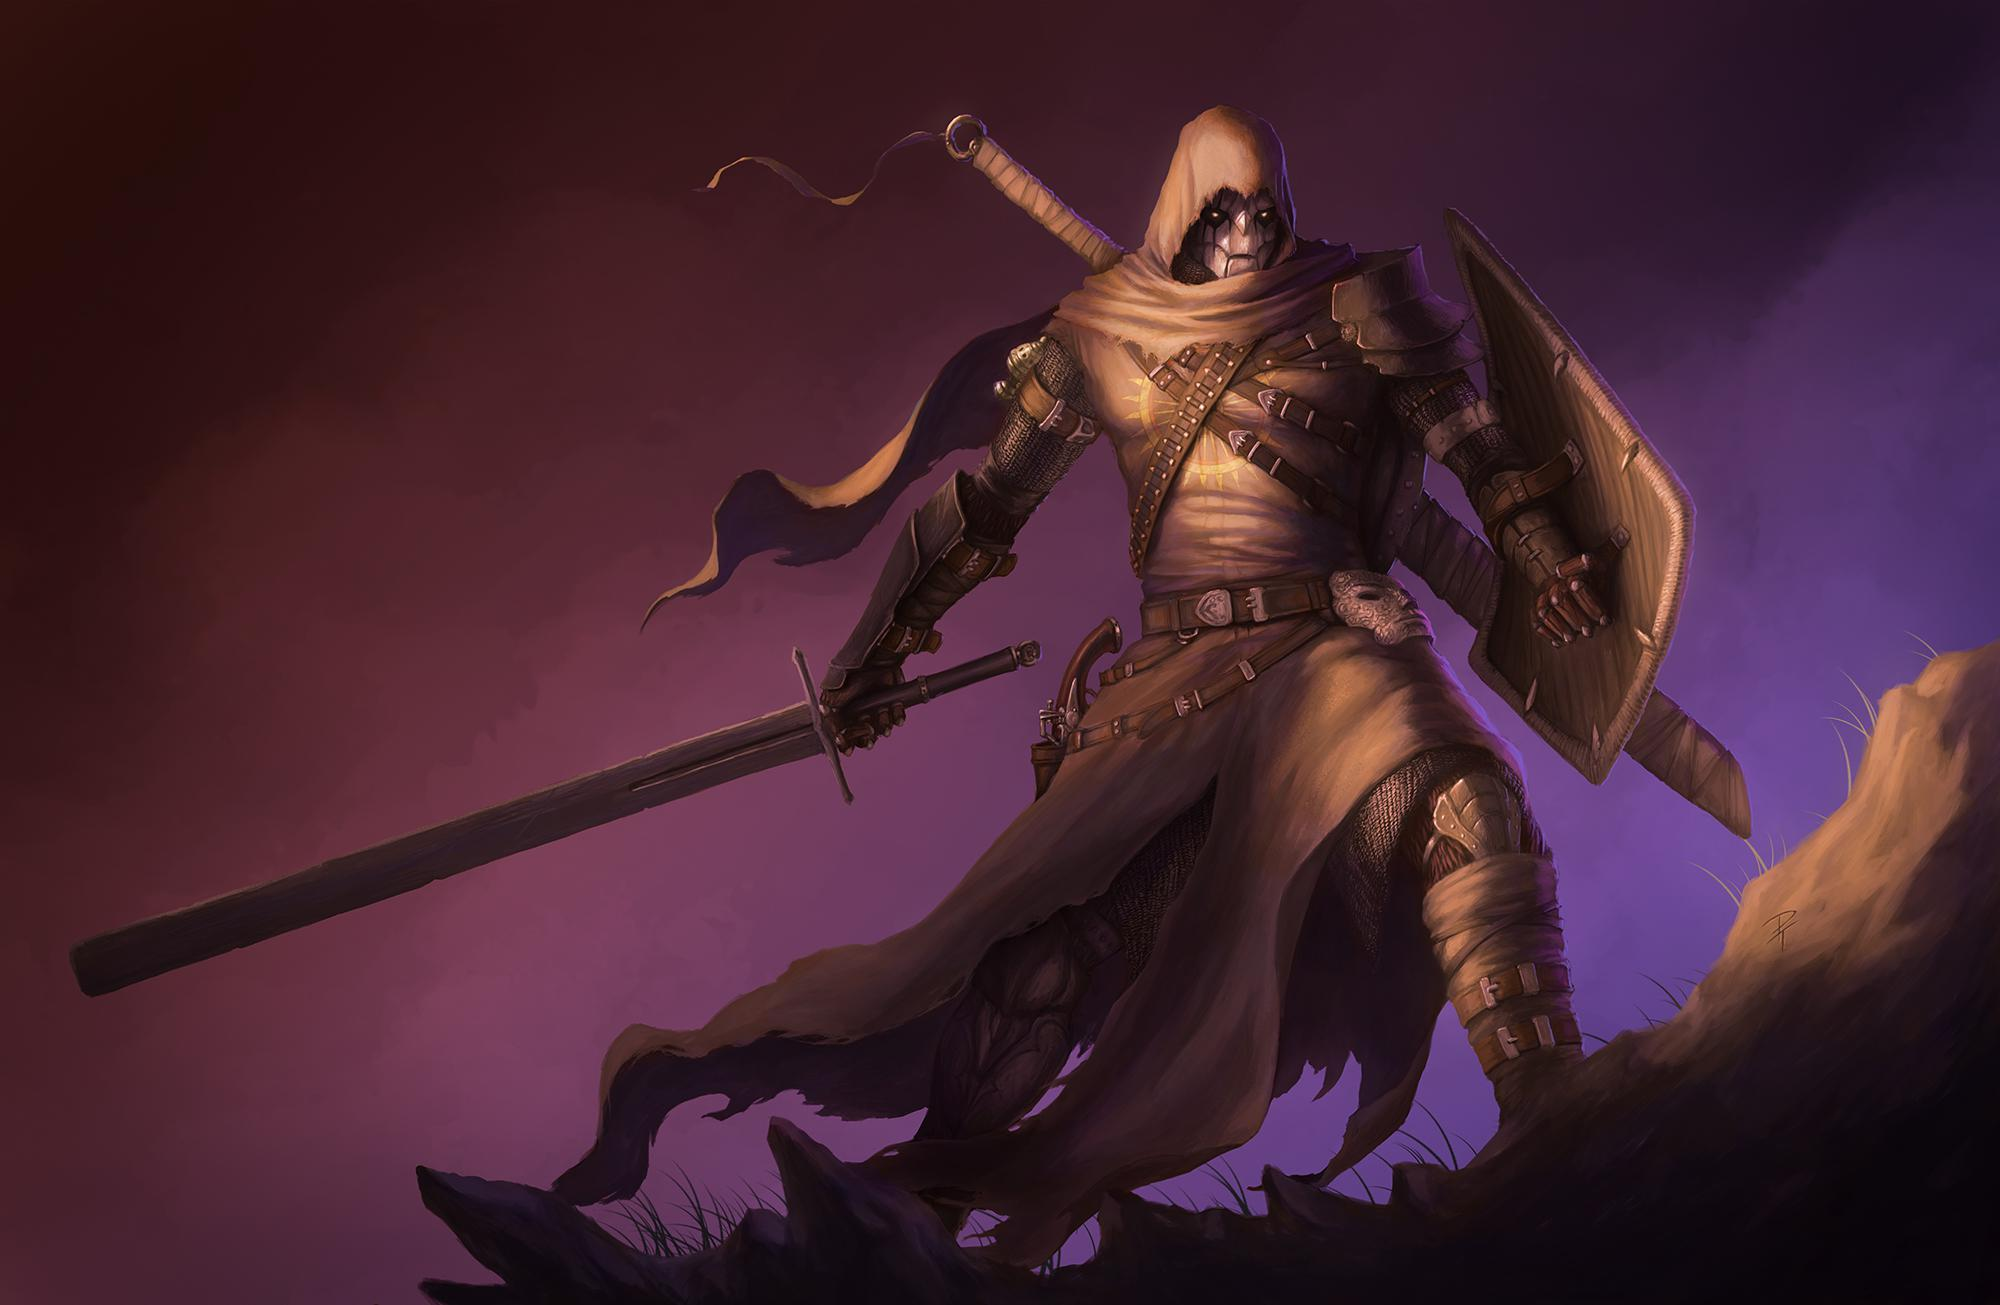
\includegraphics[width=0.98\textwidth]{03kins/img/21quies_executioner.jpg}
    \end{DndTable}
\end{table*}

\subsubsection{Slag Worker}
Even with the adaptable form of the tall kin, not even them can survive the extreme heat of lava for long.
Consequently, they created the slag workers, quies designed specifically for working inside volcanoes.
Built to work under extreme pressure, the carapace of the slag workers is a thick layer made from rhyolite.
While the rock deforms and contorts under lava, it completely blocks the quies from the liquid and its heat.
% Even the qualar of these quies is infused with the rock, to completely isolate them from their environment.

\subparagraph{Ability Score Increase} Your Constitution score increases by 1.

\subparagraph{Heavy Plating} This trait replaces integrated protection.
You are covered by a rhyolite armor of a light-pink and gray color, containing small vugs filled with obsidian and quarz.
Your Armor Class is 16 + your proficiency bonus with Heavy Armor, and you have disadvantage of Dexterity (Stealth) checks.
For all intends and purposes your natural armor is considered Heavy Armor, and it cannot be removed from your body in any way while you are alive.

\subparagraph{Specialized Worker} You are resistant to fire damage.
You are also able to enter bodies of lava or magma, sinking at a speed of 5 feet per turn and not suffering any damage while inside.
For the purposes of moving, lava and magma counts as difficult terrain for you.
You still need to breathe, and must follow the normal rules for holding your breath while submerged in the hot liquid.

\subparagraph{Defensive Stance} If you have one hand free, you can choose to enter a defensive stance as an action.
You add your proficiency bonus with an armor type of your choice until the start of your next turn.

\end{linenumbers}


    % \chapter{Walk of Life}

\DndDropCapLine{A}{part from their kin, your character}
is naturally defined by additional characteristics, such as their origin, background, and profession.
They are an individual with their own walk of life in the vast lands of Yuadrem.
This chapter explores the details separating your character from their peers, such as their name and physical description, their personality and alignment, and their origin and background.


\section{Details}

\subsection*{Name}
While your character's kin description in the previous chapter contains a list of common names, you are welcome to create your own.
For this, you can use the names in that list as a rough guideline to understand how their naming conventions usually works.

Also think about how your character obtained their name.
Each kin's section provides some information about how it's common for a member of your kin to obtain a name.
Consider if this applies to your character and think what your character thinks of their name.
Are they proud of it or do they dislike its origin or meaning?

\subsection*{Sex}
Most of the kins are genderless, and thus sex and gender don't really have relevance in most societies of Yuadrem.
If you choose to make a character of one of the gendered kins, keep in mind that their place in society will be generally unaffected.

With the exception of the qulbaba ird's feathers, your character's stats and characteristics are unaffected by their sex.

\subsection*{Height and Weight}
Based on their kin, you can decide your character's height and weight using the information in the Kins chapter.
You are encouraged to think of how your character's ability scores relate to these characteristics, or even how they may clash.

As in the PHB, you can roll randomly using the Random Height and Weight table.
The dice roll given in the Height Modifier column determines the character's extra height (in cm) beyond the base height.
Then, the dice roll given in the Weight Modifier column determines the character's extra weight (in kg) beyond the base weight.

\begin{DndTable}[width=\linewidth, header=Random Height and Weight]{lp{0.7cm}p{1.2cm}p{0.7cm}p{1.2cm}}
    \textbf{Kin} & \textbf{Base Height} & \textbf{Height Modifier} & \textbf{Base Weight} & \textbf{Weight Modifier} \\
    Gat               & 120  & 1d10 $\times$ 3  &  40  & 1d20 $\times$ 1   \\
    Treb Gat          & 160  & 1d10 $\times$ 4  &  90  & 1d10 $\times$ 3   \\
    Ird               & 170  & 1d10 $\times$ 3  &  40  & 1d10 $\times$ 1   \\
    Thulkraka Ird     & 170  & 1d10 $\times$ 3  &  60  & 1d20 $\times$ 1   \\
    Marset            &  70  & 1d10 $\times$ 3  &  18  &  1d4 $\times$ 1   \\
    Oth               & 130  & 1d10 $\times$ 5  &  40  & 1d10 $\times$ 1   \\
    Naenk             & \multicolumn{4}{l}{See Size in page \pageref{kin::naenk.size}} \\
    Tsanek            & 180  & 1d10 $\times$ 2  &  60  & 1d20 $\times$ 1   \\
    Tortle            & 150  & 1d10 $\times$ 3  & 200  & 1d20 $\times$ 3   \\
    Grung             &  75  & 1d10 $\times$ 3  &  18  &  1d4 $\times$ 1   \\
    Uman              & 150  & 1d10 $\times$ 4  &  50  & 1d10 $\times$ 3   \\
    Zaloth            & 150  & 1d10 $\times$ 3  & < 1  & -                 \\
    Quies Operative   & 180  & 1d10 $\times$ 5  &  70  & 1d20 $\times$ 4   \\
    Quies Juggernaut  & 180  & 1d10 $\times$ 5  & 200  & 1d10 $\times$ 3   \\
    Quies Slag Worker & 180  & 1d10 $\times$ 5  & 250  & 1d10 $\times$ 5
\end{DndTable}

\subsection*{Physical Characteristics}
Apart from what you've already defined, you also choose your character's age and eye, hair, and skin color.
Some characteristics specific to your character's kin are also customizable, like a gat's horns or an ird's feather patterns.

To help set apart your character from the rest, consider also giving them an unusual or memorable physical characteristic, such as a scar, a limp, or a tattoo.
Think about how your character acquired such a feature and the story they might tell to explain it.

\subsection*{Qualar}
Most people keep their qualars hidden and unadulterated.
Some, however, enjoy carving messages or drawings into theirs, so as to enjoy themselves or to be remembered by the next carrier of the bone artifact.
A few even cut small dents into it to place gems or crystal windows into the tarry liquid hidden within.

Bonecarvers capable of crafting artificial qualars usually cut them into a specific design so that people know who made them.
These designs can take many forms, like simple geometrical shapes to fine trinkets with intricate shapes.
It is usual that these qualars are more expensive than the ones made by Ctereth, and the finest ones are usually reserved only for the elite.

You are free to choose a qualar that makes sense for your character within reason.
Also consider the relation your character has with their qualar.
Perhaps they treasure it as a reminder of a home now abandoned, or maybe they want to exchange it in the first available opportunity.

\subsection*{Tidal Alignment}
To define your character's moral compass and the way they interact with the world, define one or two dominant tides for them.
The phenomenon of the tides is described in page \pageref{ssec::tides}.

Examples of people aligned to each tide follow.

\subparagraph{Blue Tide} A philosopher obsessed with the pursuit of enlightenment.
A monk seeking wisdom to pass off to their school.
A shaman making decisions for their tribe using both reason and mysticism.

\subparagraph{Red Tide} An artist looking for passionate experiences to portray.
An adventurer defying dangers in search of action and emotion.
A crusader on a zealous quest for their divinity of choice.

\subparagraph{Silver Tide} A ranger traversing an unexplored forest to leave a mark on history.
A bard seeking to influence others with their music.
A knight performing glorious deeds to acquire fame.

\subparagraph{Indigo Tide} A congressperson writing laws to improve equity in their nation.
A judge executing impartial justice to improve society as a whole.
A tyrant governing under the hood of the greater good.

\subparagraph{Gold Tide} A philanthropist aiding communities with their wealth.
A crime lord who cares for their community for their own gain.
A priest aiding the locals to gain favor from their god.

When defining your character's tidal alignment, always remember that the tides are associated to action, not intention.
Even if your character is merely seeking power, if to attain it they perform noble actions for a faction they will still improve their alignment with the gold tide.

\begin{table*}[b]%
    \begin{DndTable}[width=\linewidth]{X}
        \centering
        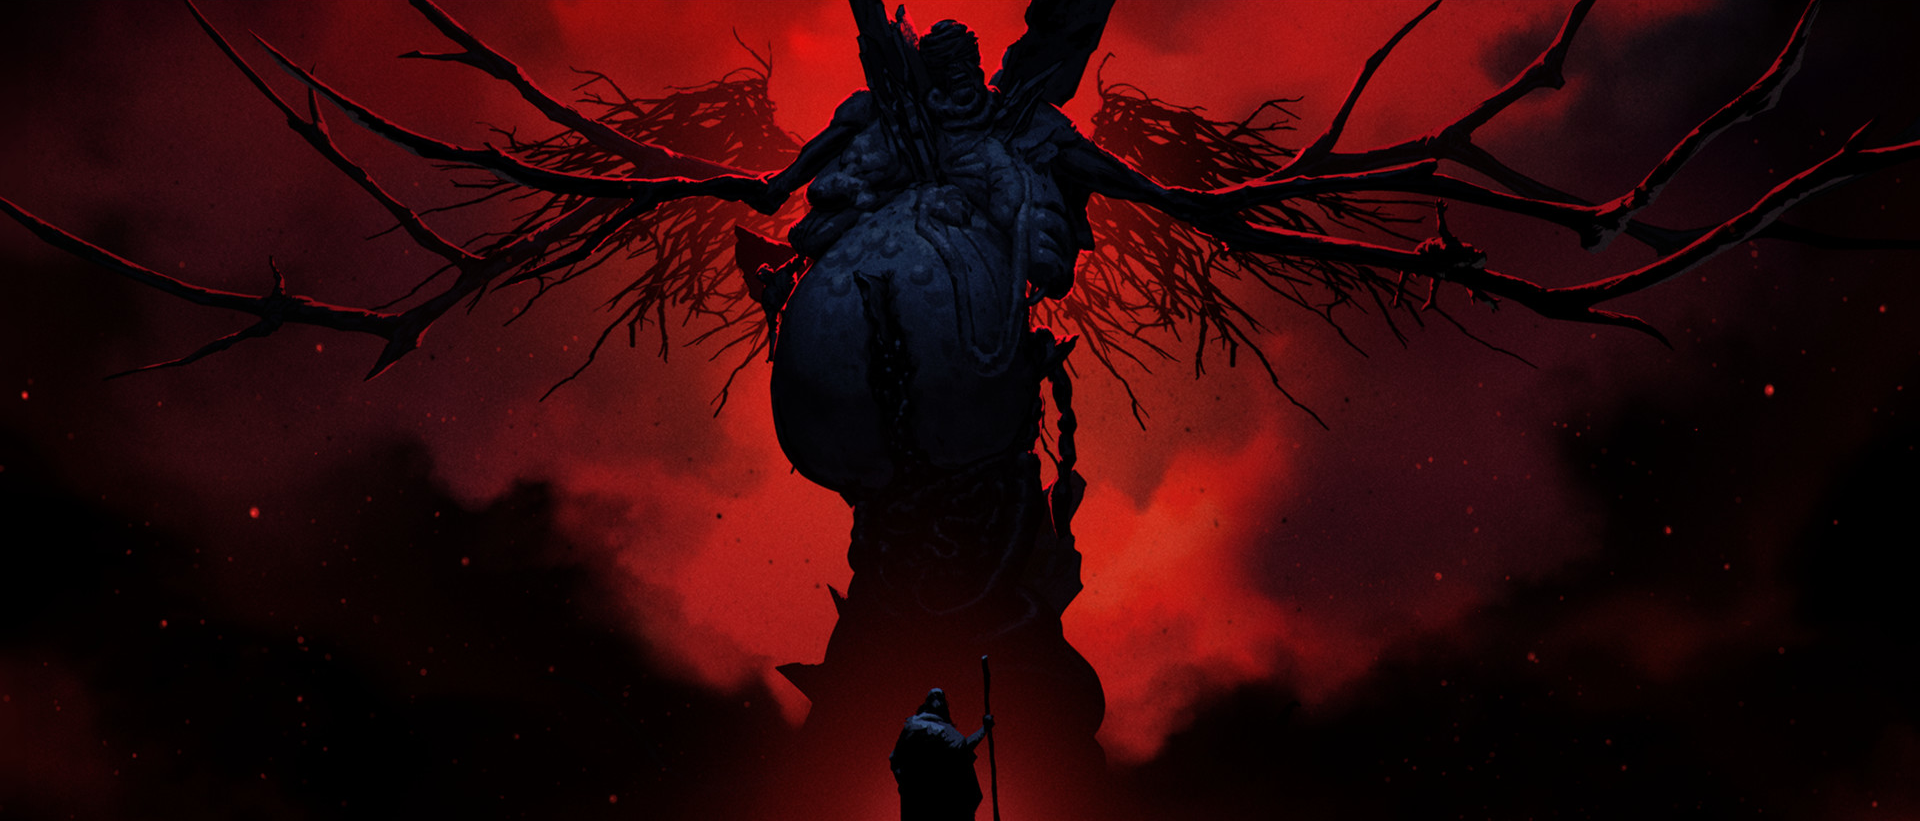
\includegraphics[width=0.95\textwidth]{04background/img/tidal_sway_rendition.png} \
        \centering \large{\textbf{Artist's Rendition of The Sorrow.}}
    \end{DndTable}
\end{table*}

\subsection*{Personal Characteristics}
For additional personal characteristics, you can follow the guidelines in pages 123 and 124 in the PHB.
You are not limited however to personality traits, ideals, bonds, and flaws.
You can flavor things as you see fit, adding attributes such as prides, dark secrets, flairs, etc.

Your character might take pride in their cooking even if they're not a professional chef.
Or they may have stolen an ancient family artifact before leaving home for adventure, claiming to have inherited it normally.
They may also be a particularly good juggler, and tend to juggle with stones when bored in a social situation.

Your character sheet includes an area to write your character's personal characteristics, but you are welcome to use additional sheets if your you need more space.
As advice, it's a good idea to put at least as much thought into your character's characteristics as you put into their appearance.

\section{Background}

For your character's background, you can choose any from some of the official D\&D5e books which fit best with your character.
The specific books from which you are welcome to pick a background are Acquisitions Incorporated, Ghosts of Saltmarsh, the Player's Handbook, Mythic Odysseys of Theros, and Tomb of Annihilation.

The only change you need to apply is to convert any initial money to the local currency of the region where you're playing.
To do this, convert the GP to the local currency using the currencies table in page \pageref{sec::currency} using the selling value.

To choose religions and learned languages, refer to their respective sections in pages \pageref{ssec::religions} and \pageref{ssec::languages}.

\section{Origins}

\DndDropCapLine{I}{n Yuadrem, your character's mother}
language and some common characteristics may be defined by their country of origin.
While not too much detail is given per country, you are welcome to speak with your DM (or the book's author!) if you need more information about a specific one.

To help you decide a country of origin or let a die roll decide it, a political map and a table of countries are given.
The table lists all countries with their common kins, common languages, and some cultural mannerisms.

The \textbf{common kin(s)} column simply represents the kin of the people you're most likely to come into when in a city, but is not an exhaustive list.

\begin{table*}[b]%
    \begin{DndTable}[width=\linewidth]{X}
        \centering
        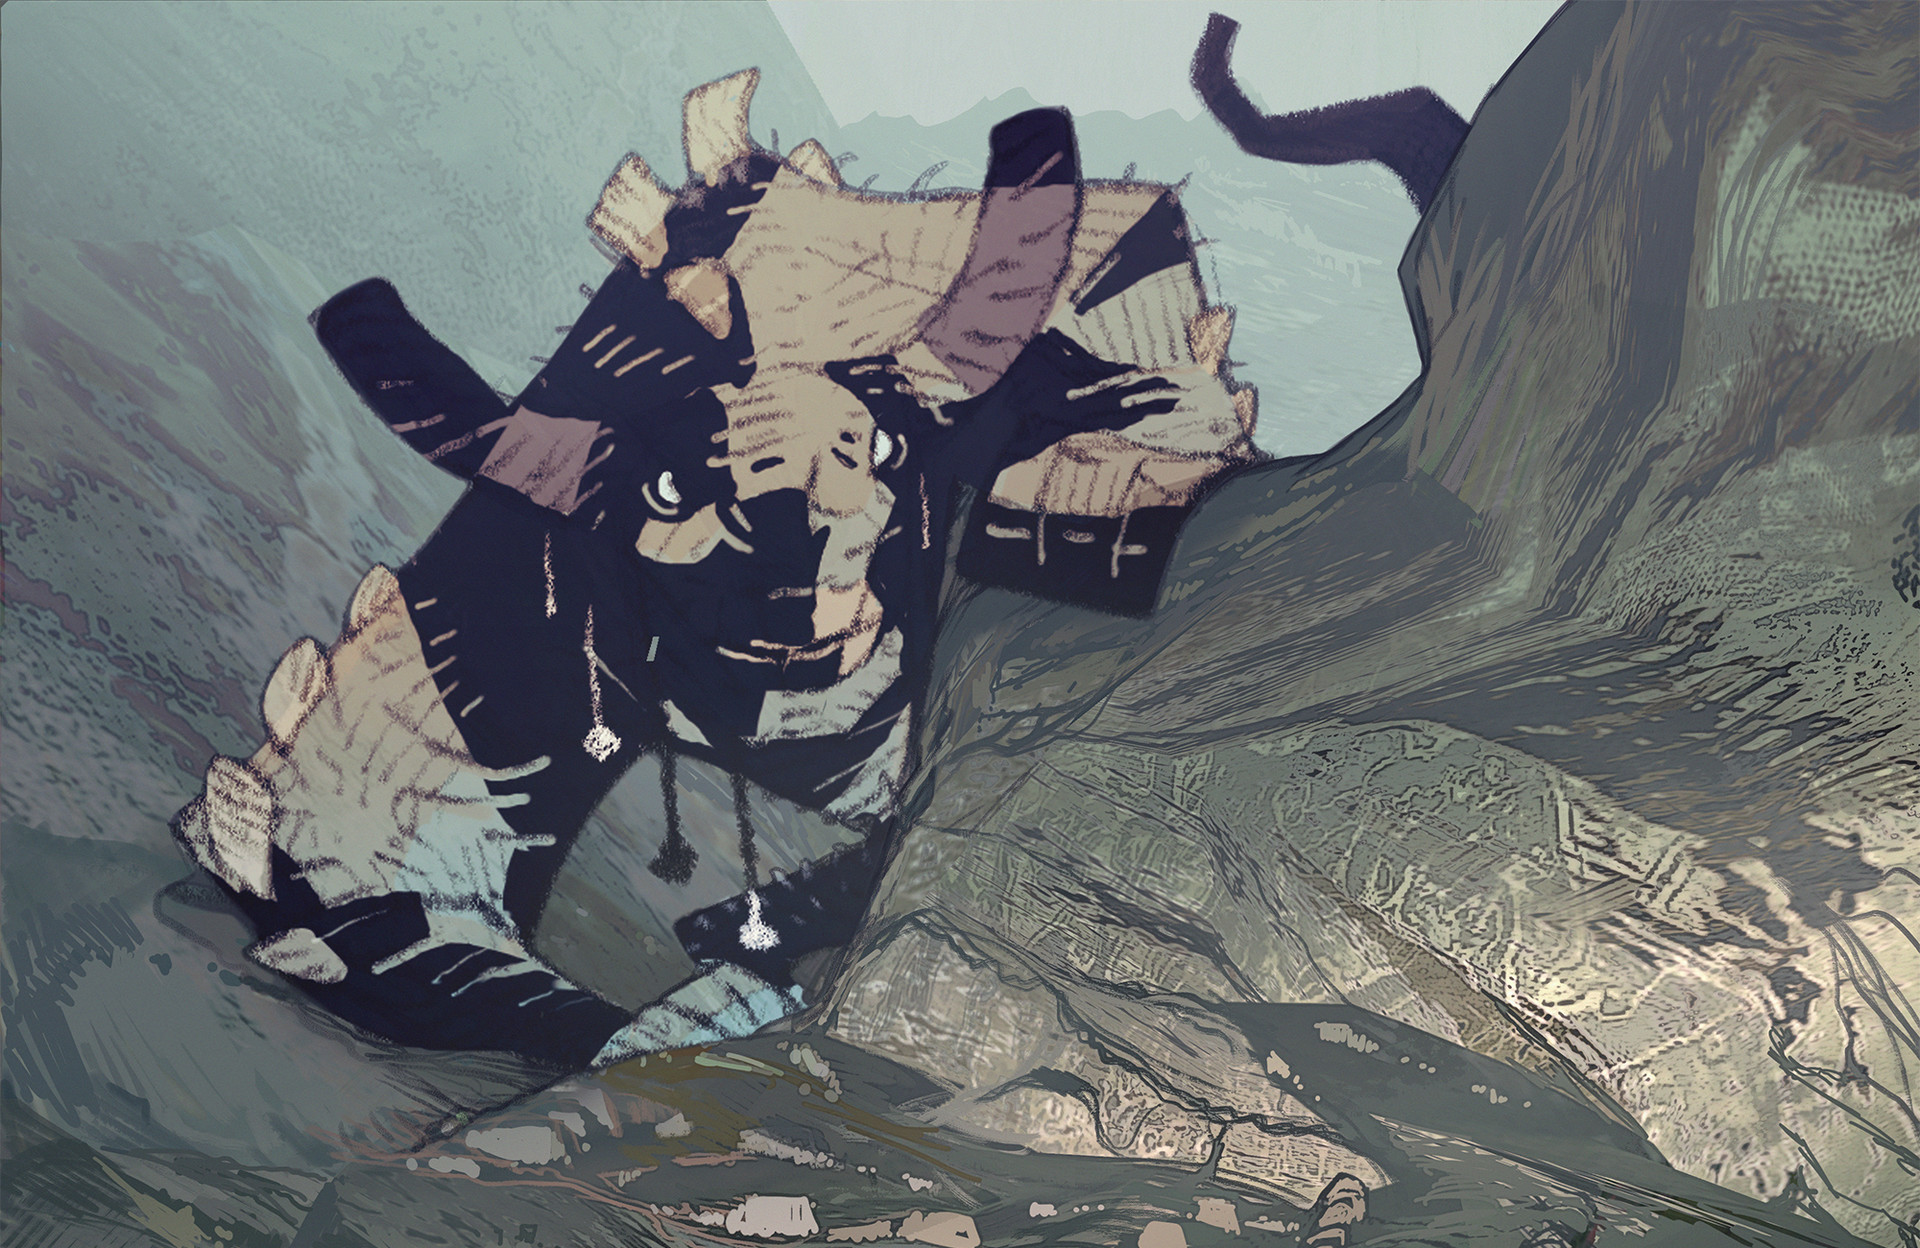
\includegraphics[width=0.95\textwidth]{04background/img/king_of_the_gray_sands_trebos.jpg} \
        \centering \large{\textbf{Trebos, King of the Gray Sands}}
    \end{DndTable}
\end{table*}

Then, the \textbf{common language(s)} column represents the most spoken (or official) language in the country, while the second or third languages in the column are commonly heard tongues among the people.

Finally, the \textbf{cultural mannerisms} column is a list of common stereotypes associated to the people of a country.
While they are not necessarily true for each particular person, your character might pride themselves or react in a certain manner to the specific characteristics attributed to their country of origin.

It's worth noting that there are six areas shown in the political map and described in the table are not exactly countries in a traditional sense, but are well-defined regions of land where for one reason or another no culture has declared their own.

The first of these is Jatuunsa, the land of the giants.
Then Nastralinal, the land of the ettins.
The Nest, home to the mysterious Fo.
The majority of the Wildlands, inhabited by the tidal creatures.
The Wurmlands, home to the wurm colonies.
And Zashlath, the insurmountable desert.

While not official countries in any degree, some nomad tribes and a few permanent settlements exist in these untamed lands, and you are more than welcome to make one of these the birthplace of your character.

If you want to let the dice decide your character's origin, roll a d6 and a d20 and use the results.
The first table in the list represents the dice rolls, in a d6,d20 format.

If the d6 lands on a 6 and the d20 on a 18, 19, or 20, you can always make your character be a late arrival.
Late arrivals can either be umans, tortles, or grungs ``coming late'' from the sizzling gate, or zaloth and quies that for any reason didn't join their kin after the schism.

\incgraph[documentpaper,][width=\paperwidth,height=\paperheight]{04background/img/political_map.png}

\begin{table*}[!ht]%
    \begin{DndTable}[width=\linewidth, header=Country List]{p{0.65cm}p{3cm}XXX}
        \textbf{Die} & \textbf{Country}           & \textbf{Common kin(s)}               & \textbf{Common Language(s)}  & \textbf{Cultural Mannerism(s)}  \\
        1, 1             & \textbf{Abababa}           & marset                               & Babazano                     & distrustful                     \\
        1, 2             & \textbf{Abipolash}         & moonborn \& chu’ash oth              & Shamabic, Fruenese           & resentful, careful              \\
        1, 3             & \textbf{Adraman}           & chu’ash oth                          & Shamabic                     & rude, defensive                 \\
        1, 4             & \textbf{Babana}            & marset, tortle                       & Babazano, Krelho             & protective, welcoming           \\
        1, 5             & \textbf{Barit}             & cliff \& bughna gat, zsek ird        & Avshenese, Zsekian           & business-minded, greedy         \\
        1, 6             & \textbf{Beilios}           & chu’ash oth                          & Shamabic                     & unwelcoming                     \\
        1, 7             & \textbf{Brovish}           & bughna gat                           & Avshenese                    & uncivilized, competitive        \\
        1, 8             & \textbf{Byurev}            & cliff \& bughna gat                  & Avshenese                    & defensive, decisive             \\
        1, 9             & \textbf{Cabb Goem Rlamesh} & varied                               & Conscript Tongue             & strange, secretive              \\
        1, 10            & \textbf{Chitsia}           & varied                               & Fruenese                     & remorseful, distrustful         \\
        1, 11            & \textbf{Dentralin}         & qulbaba ird                          & Qualinese                    & traditionalist, disciplined     \\
        1, 12            & \textbf{Diathal}           & qulbaba ird                          & Qualinese                    & defensive, indifferent          \\
        1, 13            & \textbf{Digmis}            & cliff \& bughna gat                  & Avshenese                    & resourceful                     \\
        1, 14            & \textbf{Dnimas}            & treb gat, zsek ird                   & Avshenese, Zsekian           & traditional, conniving          \\
        1, 15            & \textbf{Dnomit}            & cliff gat                            & Avshenese                    & faint-hearted, broad-minded     \\
        1, 16            & \textbf{Drer}              & varied                               & Fruenese                     & impulsive, creative             \\
        1, 17            & \textbf{Dzarog}            & treb gat, cursed uman                & Avshenese, Jantherlin        & mysterious, calm                \\
        1, 18            & \textbf{Dzokrenar}         & thulkraka \& zsek ird                & Harualish, Zsekian           & religious, traditionalist       \\
        1, 19            & \textbf{Edede}             & marset                               & Babazano                     & distrustful, protective         \\
        1, 20            & \textbf{Erpat}             & bughna gat                           & Avshenese                    & curious, aggressive             \\
        2, 1             & \textbf{Esketis}           & cliff gat, thulkraka ird             & Shanise, Avshenese           & distrustful                     \\
        2, 2             & \textbf{Faros}             & chu’ash oth                          & Shamabic                     & carefree                        \\
        2, 3             & \textbf{Fobros}            & bughna gat                           & Avshenese                    & hardworking, violent            \\
        2, 4             & \textbf{Folhoghit}         & cliff gat, thulkraka ird             & Avshenese                    & traditionalist, business-minded \\
        2, 5             & \textbf{Fraid}             & chu’ash oth, zsek ird                & Shamabic, Zsekian            & friendly, trusting              \\
        2, 6             & \textbf{Froibias}          & moonborn oth                         & Shamabic                     & hardworking                     \\
        2, 7             & \textbf{Gannag}            & naenk, tsanek                        & Knaenese                     & protective                      \\
        2, 8             & \textbf{Geanal}            & thulkraka ird                        & Harualish                    & religious, defensive            \\
        2, 9             & \textbf{Gethog}            & bughna gat, oth                      & Fruenese, Avshenese          & defensive, resentful            \\
        2, 10            & \textbf{Giothal}           & thulkraka ird, common uman           & Shanise, Odhualen            & progressive, friendly           \\
        2, 11            & \textbf{Glameas}           & moonborn oth                         & Shamabic                     & organized, competitive          \\
        2, 12            & \textbf{Gronselar}         & thulkraka ird, moonborn oth, tortle  & Harualish                    & proud, defensive                \\
        2, 13            & \textbf{Guadol}            & zsek ird                             & Zsekian                      & conniving, unrelenting          \\
        2, 14            & \textbf{Harual}            & qulbaba ird, marset                  & Harualish, Babazano          & traditionalist, protective      \\
        2, 15            & \textbf{Hianish}           & zsek ird                             & Zsekian                      & secretive, strategic            \\
        2, 16            & \textbf{Huada}             & zsek \& qulbaba ird                  & Zsekian, Qualinese           & curious, resourceful            \\
        2, 17            & \textbf{Hurzen}            & thulkraka \& zsek ird                & Harualish, Zsekian           & protective, stealthy            \\
        2, 18            & \textbf{Ignelli}           & moonborn oth                         & Shamabic                     & careful, controlling            \\
        2, 19            & \textbf{Isken}             & grung                                & Krelho                       & aggressive, racist              \\
        2, 20            & \textbf{Jatuunsa}          & giants, trolls                       & -                            & -                               \\
        3, 1             & \textbf{Jenkash}           & qulbaba \& zsek ird                  & Qualinese, Zsekian           & conservative                    \\
        3, 2             & \textbf{Jinnegh}           & bughna gat                           & Avshenese                    & industrious, defensive          \\
        3, 3             & \textbf{Jooltes}           & zsek \& qulbaba ird                  & Zsekian, Qualinese           & resourceful, curious            \\
        3, 4             & \textbf{Jualnar}           & thulkraka \& zsek ird                & Harualish, Zsekian           & isolated, religious             \\
        3, 5             & \textbf{Kaldrathal}        & thulkraka ird                        & Shanise                      & innovative, business-minded     \\
        3, 6             & \textbf{Katnak}            & bughna gat                           & Avshenese                    & violent                         \\
        3, 7             & \textbf{Keeran}            & zsek ird                             & Zsekian                      & resentful, cold                 \\
        3, 8             & \textbf{Khedrat}           & cliff gat                            & Avshenese                    & conservative, hardworking       \\
        3, 9             & \textbf{Khesol}            & cliff \& bughna gat, zsek ird        & Avshenese, Zsekian           & absent-minded, carefree         \\
        3, 10            & \textbf{Khudel}            & cliff gat, thulkraka ird             & Shanise, Avshenese           & friendly, curious               \\
        3, 11            & \textbf{Krudzal}           & thulkraka ird                        & Shanise                      & industrious, conservative       \\
        3, 12            & \textbf{Kuasesh}           & zsek ird, treb gat                   & Zsekian, Avshenese           & violent, oppressive             \\
        3, 13            & \textbf{Loods}             & zsek ird                             & Zsekian                      & cold, strategic                 \\
        3, 14            & \textbf{Mbeat}             & tortle, cliff gat                    & Krelho, Avshenese            & positive, welcoming             \\
        3, 15            & \textbf{Meghritan}         & cliff gat                            & Avshenese                    & indecisive, calm                \\
        3, 16            & \textbf{Na’ane}            & tsanek, naenk                        & Knaenese                     & industrious, progressive        \\
        3, 17            & \textbf{Nalash}            & zsek ird                             & Zsekian                      & elitist, aggressive             \\
        3, 18            & \textbf{Naptane}           & varied                               & Avshenese                    & broad-minded, friendly          \\
    \end{DndTable}
\end{table*}
\begin{table*}[h!]%
    \begin{DndTable}[width=\linewidth, header=Country List (cont.)]{p{0.65cm}p{1.5cm}p{5.5cm}XX}
        3, 19            & \textbf{Nashtralinal}      & ettins, trolls                       & -                            & -                               \\
        3, 20            & \textbf{Ndancat}           & thulkraka ird                        & Shanise                      & curious                         \\
        4, 1             & \textbf{Niadsona}          & zsek ird, treb gat                   & Zsekian, Avshenese           & resourceful, curious            \\
        4, 2             & \textbf{Nimastan}          & treb \& bughna gat, zsek ird         & Avshenese, Frishian, Zsekian & naturalistic, violent           \\
        4, 3             & \textbf{Nuaqlon}           & thulkraka ird                        & Shanise                      & community-oriented              \\
        4, 4             & \textbf{Nubefora}          & bughna gat                           & Avshenese                    & aggressive                      \\
        4, 5             & \textbf{Padmui}            & common uman, thulkraka ird           & Odhualen, Shanise            & progressive                     \\
        4, 6             & \textbf{Palegna}           & moonborn \& chu’ash oth              & Shamabic, Fruenese           & rational, extremist             \\
        4, 7             & \textbf{Pebos}             & treb \& bughna gat, zsek ird         & Avshenese, Frishian, Zsekian & aggressive, proud               \\
        4, 8             & \textbf{Phravat}           & bughna gat                           & Avshenese                    & curious, honorable              \\
        4, 9             & \textbf{Ptemos}            & cliff \& bughna gat                  & Avshenese                    & curious, disorganized           \\
        4, 10            & \textbf{Pthox}             & cliff gat, thulkraka ird             & Shanise, Avshenese           & industrious, absent-minded      \\
        4, 11            & \textbf{Raraspan}          & treb gat, zsek ird                   & Avshenese, Zsekian           & aggressive, competitive         \\
        4, 12            & \textbf{Rhuashodo}         & marset                               & Jantherlin                   & secretive, controlling          \\
        4, 13            & \textbf{Ribinhep}          & common \& frost uman                 & Odhualen, Frost Tongue       & aggressive, resentful           \\
        4, 14            & \textbf{Rona}              & thulkraka ird, cliff gat             & Shanise                      & business-minded, open           \\
        4, 15            & \textbf{Seesh}             & zsek ird, treb gat                   & Zsekian, Avshenese           & aggressive, competitive         \\
        4, 16            & \textbf{Shaghdemk}         & varied                               & Avshenese                    & relaxed, careless               \\
        4, 17            & \textbf{Shianasal}         & qulbaba ird                          & Qualinese                    & aggressive, defensive           \\
        4, 18            & \textbf{Shief}             & sunstruck oth                        & Shamabic                     & secretive                       \\
        4, 19            & \textbf{Shimfor}           & treb gat, zsek ird                   & Avshenese, Zsekian           & disorganized, resentful         \\
        4, 20            & \textbf{Shtebin}           & bughna gat                           & Avshenese                    & hardworking, hot-tempered       \\
        5, 1             & \textbf{Shuas}             & zsek ird                             & Zsekian                      & resentful, hot-tempered         \\
        5, 2             & \textbf{Shulnar}           & zsek ird                             & Zsekian                      & traditionalist, resentful       \\
        5, 3             & \textbf{Siaden}            & zsek ird                             & Zsekian                      & resourceful, conniving          \\
        5, 4             & \textbf{Sirilio}           & chu’ash oth                          & Shamabic                     & rude, defensive                 \\
        5, 5             & \textbf{Skiod}             & moonborn oth, qulbaba ird            & Shamabic                     & careful, slow                   \\
        5, 6             & \textbf{Sklianmui}         & common uman, thulkraka ird, zaloth   & Odhualen, Shanise            & progressive, industrious        \\
        5, 7             & \textbf{Skruan}            & tortle, thulkraka ird                & Krelho, Harualish            & melancholic, adventurous        \\
        5, 8             & \textbf{Stendal}           & thulkraka ird                        & Shanise                      & traditional, leading            \\
        5, 9             & \textbf{Stuksher}          & bughna gat                           & Avshenese                    & curious, competitive            \\
        5, 10            & \textbf{Sulia}             & varied                               & Fruenese                     & industrious, liberal            \\
        5, 11            & \textbf{Tadnas}            & zsek ird                             & Zsekian                      & defensive                       \\
        5, 12            & \textbf{Tashta}            & bughna gat                           & Avshenese                    & hardworking, aggressive         \\
        5, 13            & \textbf{Thaidzar}          & thulkraka ird, tortle                & Harualish, Krelho            & careful, friendly               \\
        5, 14            & \textbf{Thalrog}           & treb \& bughna gat, zsek ird         & Avshenese, Frishian, Zsekian & strategic, proud                \\
        5, 15            & \textbf{The Nest}          & ???                                  & ???                          & ???                             \\
        5, 16            & \textbf{Thig}              & bughna gat                           & Avshenese                    & distrustful, resentful          \\
        5, 17            & \textbf{Tiadsol}           & zsek ird, treb gat, cursed uman      & Zsekian, Avshenese, Odhualen & disorganized, strong-willed     \\
        5, 18            & \textbf{Tidsaim}           & moonborn oth                         & Shamabic                     & secretive, careful              \\
        5, 19            & \textbf{Tlondez}           & thulkraka \& zsek ird                & Harualish, Zsekian           & friendly                        \\
        5, 20            & \textbf{Tñaas}             & zsek ird                             & Zsekian                      & carefree                        \\
        6, 1             & \textbf{Traigar}           & thulkraka ird, bughna gat            & Shanise, Avshenese           & religious, curious              \\
        6, 2             & \textbf{Treberos}          & varied                               & Avshenese, Fruenese          & broad-minded, determined        \\
        6, 3             & \textbf{Ushpavam}          & cliff gat, tortle                    & Avshenese, Krelho            & friendly                        \\
        6, 4             & \textbf{Vamerit}           & cliff gat                            & Avshenese                    & organized                       \\
        6, 5             & \textbf{Vieigesh}          & moonborn \& chu’ash oth, bughna gat  & Shamabic, Fruenese           & careful, ever-ready             \\
        6, 6             & \textbf{Viphoger}          & cliff gat                            & Avshenese                    & industrious, broad-minded       \\
        6, 7             & \textbf{Visilias}          & moonborn oth                         & Shamabic                     & curious, traditional            \\
        6, 8             & \textbf{Voskferm}          & cliff gat                            & Voskian                      & proud, strong-willed            \\
        6, 9             & \textbf{Voskgrit}          & cliff gat                            & Voskian                      & industrious, defensive          \\
        6, 10            & \textbf{Wildlands}         & tidal creatures                      & ???                          & -                               \\
        6, 11            & \textbf{Wurmlands}         & wurms                                & Silent Speech                & -                               \\
        6, 12            & \textbf{Xarjage}           & cliff gat, boggart                   & Avshenese, Bog Tongue        & conservative, relaxed           \\
        6, 13            & \textbf{Zashlath}          & -                                    & -                            & -                               \\
        6, 14            & \textbf{Zealar}            & thulkraka ird                        & Shanise                      & honest, hardworking             \\
        6, 15            & \textbf{Zigpor}            & bughna gat                           & Avshenese                    & disorganized, competitive       \\
        6, 16            & \textbf{Zimted}            & chu’ash oth                          & Shamabic                     & carefree, curious               \\
        6, 17            & \textbf{Zmiva}             & sunstruck oth                        & Shamabic                     & aggressive
    \end{DndTable}
\end{table*}

\newpage~\newpage


    % % !TEX root = ../main.tex
\chapter{Mechanic Changes}
\begin{linenumbers}
\DndDropCapLine{S}{trans may break alone, but twisted}
\textit{make a braid. All are not the same, but they shall be as one.
The journey shall be made.}

\hspace*{\fill} --- Anonymous song.

This book includes major mechanical changes.
These mostly focus on allowing players to embrace the worldbuilding aspects of Yuadrem by freeing up their character building options.
These changes are of course optional, but most of the rules in the book were designed with them in mind.

Then, optional rules are included.
Yuadrem is a harsh continent, and these rules help set the atmosphere to reflect this.
They are completely optional, and a healthy gaming table should discuss which should be included or excluded in their game.

\begin{DndComment}{Help Wanted!}
    This entire book was designed with the major mechanical changes considered, yet the author realizes that this can alienate a large part of the community.
    You may want to play in Yuadrem without these changes.
    If this is the case, it is recommended that change many mechanical aspect of the book to acommodate this.

    If for some insane reason you want to take on this challenge, you are encouraged to contact the book's author.
    We could work together on this, discussing appropiate retribution and co-authorship terms.
\end{DndComment}

% \section{Dementia}
% \DndDropCapLine{H}{arsh is the process that awaits the}
% foolish or unlucky enough to lose their qualar.
% Their sentience slips away slowly as they lose their mental capacities.
% Perhaps the worst part is that inward awareness is one of the last attributes lost, forcing them to be fully conscious of the process.
%
% The road towards dementia comes in seven stages, each roughly lasting a week.
% At the moment when you lose your qualar, you enter the first stage of dementia.
% After a week, you roll a DC 15 Intelligence saving throw.
% On a fail, you enter the next stage of dementia.
% On a success, you stay on your current stage and roll again at the start of the next week.
% Dementia is unavoidable, and the DC increases by 1 after every successful roll.
%
% \subsubsection{First Stage}
% No obvious signs of dementia, only minor short-memory loss occurs.
% The main symptoms are associated to the anxiety from the loss of the qualar.
% You start focusing more on your past, often drifting away into daydreams.
%
% You suffer the following effects:
% \subparagraph{Decreased Awareness} You roll for initiative and Dexterity saving throws with disadvantage.
% \subparagraph{Restlessness} Roll an DC 12 intelligence saving throw right after a short rest.
% On a success, you recover your hit points normally.
% On a failure, you only recover half of the hit dice rolled (rounded down).
%
% \subsubsection{Second Stage}
% The self realization and awareness that something is wrong settles in.
% You refuse to accept that your mind is slipping away.
% The more effort you put on remembering the more deterioration your memory suffers.
% Confusion starts setting in.
%
% In addition to the effects of the first stage, you suffer the following effects:
% \subparagraph{Lack of Recollection} Any ability check made to remember or recollect a memory is done with disadvantage.
% All Intelligence (History) checks are made with disadvantage.
% \subparagraph{Mood Swings} All Charisma ability checks and saving throws are made with disadvantage.
%
% \subsubsection{Third Stage}
% You experience increased forgetfulness and might find concentrating difficult.
% You are presented with some of the last coherent memories before confusion fully rolls in.
% Some singular memories become more disturbed, isolated, broken, and distant.
% These are the last embers of awareness.
%
% In addition to the effects of the last stages, you suffer the following effects:
% \subparagraph{Decreased Concentration} All Constitution saving throws made to maintain concentration are made with disadvantage.
% \subparagraph{Vagrant Mind} Intelligence and Wisdom ability checks and saving throws are rolled with disadvantage.
%
% \subsubsection{Fourth Stage}
% Grey mists form and fade away in your memory.
% The ability to recall singular memories gives way to confusion and horror.
% You struggle with daily tasks, presenting clear cognitive problems.
%
% In addition to the effects of the last stages, you suffer the following effects:
% \subparagraph{Motor Difficulties} Strength and Dexterity ability checks and saving throws are rolled with disadvantage.
% Attack rolls are made with disadvantage.
% \subparagraph{Drifting Conscience} In combat, roll a DC 8 Intelligence saving throw at the start of every turn.
% On a failure, you forget where you are, and cannot take any actions during the turn.
%
% \subsubsection{Fifth Stage}
% You have major memory deficiencies.
% The few lapses of consciousness you get are filled with dread, as you realize your mind has mostly left you.
% The repetition and rupture gives way to calmer moments, as the unfamiliar becomes familiar.
%
% In addition to the effects of the last stages, you suffer the following effects:
% \subparagraph{Loss of Fortitude} All rolls are made with disadvantage.
% \subparagraph{Complete Unawareness} All Intelligence (Investigation), Wisdom (Insight), and Wisdom (Perception) automatically fail.
% Your passive investigation, insight, and perception become 0.
%
% \subsubsection{Sixth Stage}
% Your mental state is beyond description.
% You struggle to remember your early life, even forgetting the names of your family and fellows.
% Your capacity of speech is severely impaired, and you suffer sudden and radical personality and emotional changes.
%
% In addition to the effects of the last stages, you suffer the following effects:
% \subparagraph{Declining Speech} You automatically fail all Charisma ability checks and saving throws, and have a very hard time communicating verbally.
% \subparagraph{Hope Lost} As your conscious mind fights your natural tendencies, you automatically fail death saving throws.
%
% \subsubsection{Final Stage}
% Everywhere, an empty bliss.
%
% You make what will most likely be your last die roll, this time with no disadvantage.
% Roll a d20 on the post-dementia table.
% You suffer the effect rolled.
%
% \begin{DndTable}[width=\linewidth, header=Post-dementia Effects]{lX}
%     \textbf{Roll} & \textbf{Effect} \\
%     1 & Your last emotion is rage. You become mindless and violent, attacking your companions without reason. \\
%     2-5 & Your last emotion is apathy. You endlessly stare at the east until you die of natural causes. \\
%     6-18 & Even after brain death, you seek survival. You wander off, attacking any who try to stop you. You become a lost one. \\
%     19 & With memories gone, your mind is fully pulled by its tidal impulses. You lose control of your character, who becomes a servant of The Sorrow. \\
%     20 & Go back to the first stage of dementia, and gain a rank in the Dementia Insight heroic talent.
% \end{DndTable}
%
% The only conventional way to remove dementia is to obtain a qualar again.
% When this happens, you go back one stage of dementia per day passed.
% While in this state you suffer a terrible fever.
% At the beginning of each day roll a Constitution saving throw.
% On a failure, you gain one level of exhaustion.
%
% \section{Hardcore Rules}
% \subsection*{Critical Hits}
%
% \subsection*{Encumbrance}
%
% \subsection*{Hunger and Thirst}
%
% \subsection*{Minor and Major Injuries}
%
% \subsection*{Only One Chance}
% As a rule, you only have one chance to succeed in any action.
% Once you have rolled the dice, you many not roll again to achieve the same goal.
% You need to try something different or wait until the circumstances have changed in a substantial way.
% Or let another PC try.
%
% This rule does not apply to combat, where you can attack the same enemy until it becomes a bloody pulp.
%
% \subsubsection*{Opportunity Attacks}
% In a fight, everyone is constantly watching for enemies to drop their guard.
% While heedless movement is easily punished, any lack of concentration or unplanned action can have devastating consequences.
% Various actions provoke opportunity attacks from a creature:
% \begin{itemize}
%     \item Moving out of the creature's reach.
%     This doesn't apply when someone or something moves you without using your movement, action, or reaction.
%     \item Picking up an item from the floor while in the creature's reach.
%     \item Unsheathing a weapon while in the creature's reach.
%     \item Donning or doffing a shield while in the creature's reach.
%     \item Using the Attack action with a ranged weapon in a creature's reach.
% \end{itemize}
% You can avoid opportunity attacks during your turn by taking the Disengage action.
%
% \subsection*{Short and Long Rests}
%
% \subsection*{Stamina}

\end{linenumbers}

    % \chapter{Equipment} \label{ch::equipment}
\section{Starting Equipment} \label{sec::starting}
\section{Currency \& Trade Goods} \label{sec::currency}
\section{Armor and Shields} \label{sec::armor}
% https://2e.aonprd.com/Armor.aspx
% https://2e.aonprd.com/Shields.aspx
\section{Weapons} \label{sec::weapons}
% SPECIAL WEAPONS:
% * Huge Krudzal weapons used to fight giants
% * Drer fire weapons
% * Sulia's large blast weapons (cannons and large handcannons)
% * Kaldrathal's more refined flintlock pistols
% * Mercury weapons from frostburn umans

% heavy shields grant +3 AC and half cover against ranged attacks, but impose a movement speed debuff:
% tower shield: +3 AC, -10 movement speed
% bulwark: +4 AC, -20 movement speed

% WEAPON CATEGORIES:
% Knives:
%   simple    : dagger (L) 1d4, throwing dagger (L) 1d4, kukri 1d6 (only when thrown, less range)
%   1-handed  : parrying dagger 1
% Straight Swords:
%   simple    : shortsword 1d6
%   1-handed  : broadsword (H) 1d8, backsword 1d8
%   versatile : bastard sword 1d8-1d10
%   2-handed  : longsword 1d10, claymore (H) 1d12, zweihander (H) 2d6, flamberge (H) 1d10, greatsword (H) 2d6
% Curved Swords:
%   simple    : sickle (L) 1d4, cutlass 1d6
%   1-handed  : scimitar (L) 1d6, sabre 1d8, khopesh 1d6
%   versatile : falchion (H) 1d8-1d10
%   2-handed  : katana 1d10, double-bladed scimitar 2d4
% Light Swords:
%   simple    : mail breaker 1d4
%   1-handed  : rapier 1d8, estoc/tuck 1d8, basket hilted sword 1d8
% Axes:
%   simple    : handaxe (L) 1d6
%   versatile : battleaxe 1d8-1d10, broad axe 1d8-1d10 (H)
%   2-handed  : bearded axe 1d10, greataxe (H) 1d12
% Hammer:
%   simple    : club (L) 1d4, light hammer (L) 1d4, mace 1d6
%   1-handed  : warhammer 1d8-1d10, boomerang 1d4
%   2-handed  : greatclub (H) 1d8, maul (H) 2d6, lucerne 1d10
% Pick:
%   simple    : kama (L) 1d6
%   1-handed  : war pick 1d8
%   2-handed  : horseman's pick 1d10
% Staves:
%   simple    : quarterstaff 1d6-1d8
% Spears:
%   simple    : javelin 1d6, trident 1d6-1d8
%   versatile : spear 1d8-1d10, lance 1d12
%   2-handed  : pike (H) 1d10
% Halberds:
%   2-handed  : glaive (H) 1d10, poleaxe (H) 1d10, lucerne (H) 1d0
% Flails:
%   1-handed  : nunchaku (L) 1d4, ball-and-chain 1d6
% Whip:
%   1-handed  : whip 1d4, bullwhip (1d4 slashing but 6m reach), qilinbian (1d6 slashing, finesse, reach - 6mt)
% Bow:
%   2-handed  : shortbow 1d6, composite bow 1d8, longbow (H) 1d8, yumi (H) 1d10 - disadvantage on less than 6 meters
% Crossbow:
%   1-handed  : hand crossbow (L) R1 1d6
%   2-handed  : light crossbow R1 1d8, repeating crossbow R3 1d8, heavy crossbow (H) R1 1d10
% Pistol:
%   1-handed  : flintlock R1 1d10, pistol (change name) R4 1d8
% Musket:
%   2-handed  : musket R1 1d12
% "Newer" Firearms:
%   1-handed  : palm pistol (L) R1 1d8, pepperbox R6 1d10
%   2-handed  : blunderbuss R1 2d8, bad news R1 2d12
% Fire-breathers (Drer) - misfiring damages you:
%   1-handed  : bomb 3d6
%   2-handed  : firelance 1d12, hand mortar 2d8, flamespewer 1d6*
% Giant-slayers (Krudzal) - no extra attack:
%   2-handed  : dreihander 2d12, greatmaul 4d6, greatchisel 2d8*, hand ballista 2d10
%       dreihander    - https://mortalshell.wiki.fextralife.com/Martyr's+Blade
%       greatmaul     - https://mortalshell.wiki.fextralife.com/Smoldering+Mace
%       greatchisel   - https://mortalshell.wiki.fextralife.com/Hammer+and+Chisel
%       hand ballista - https://mortalshell.wiki.fextralife.com/Ballistazooka - action to shoot, action to reload
% Trick weapons: take 3 or 4 from here https://bloodborne.wiki.fextralife.com/Weapons.
% Exotic:
%   1-handed  :
%   versatile :
%   2-handed  : swordspear* (H) 1d10
%   ranged    : blowgun 1, net -
% Special (no specific talents, generally used for flavor):
%   simple    : shortspear 1d6, dart 1d4, sling 1d4
% Footnotes:
% * swordspears are essentially fancy glaive, but require proficiency with spears and swords due to having a different combat style.

% Take firearms from https://www.dndbeyond.com/subclasses/gunslinger .

\subsection*{Armor Properties}
\subparagraph{Bulwark} The armor covers you so completely that your movement is hindered.
You do not add your Dexterity modifier to Dexterity saving throws.

\subparagraph{Chain} The armor is so flexible that it bends under strong blows, absorbing some of their strength.
You gain resistance to the damage made by critical hits from bludgeoning, slashing, an piercing damage.

\subparagraph{Cloth} This armor is light and comfortable.
You can rest normally while wearing it.

\subparagraph{Composite} The numerous overlapping pieces of this armor protect you from piercing attacks.
You gain resistance to piercing damage.

\subparagraph{Leather} The thick second skin of the armor disperses blunt force.
You gain resistance to bludgeoning damage.

\subparagraph{Noisy} The armor is also loud and likely to alert others of your presence, giving you disadvantage on Dexterity (Stealth) checks.

\subparagraph{Plate} The sturdy plate provides no purchase for a cutting edge.
You gain resistance to slashing damage.

\subsection*{Weapon Properties}
\subparagraph{Ammunition} You can use a weapon that has the ammunition property to make a ranged attack only if you have ammunition to fire from the weapon.
Each time you attack with the weapon, you expend one piece of ammunition.
Drawing the ammunition from a quiver, case, or other container is part of the attack.
Loading a one-handed weapon requires a free hand.
At the end of the battle, you can recover half your expended ammunition by taking a minute to search the battlefield.

If you use a weapon that has the ammunition property to make a melee attack, you treat the weapon as an improvised weapon.
A sling must be loaded to deal any damage when used in this way.

\subparagraph{Explosive} Upon a hit, everything within 5 ft of the target must make a Dexterity saving throw (DC equal to 8 + your proficiency bonus + your Dexterity modifier) or suffer 1d8 fire damage.
If the weapon misses, the ammunition fails to detonate, or bounces away harmlessly before doing so.

\subparagraph{Great} This weapon requires the Great Weapon User 1 feat to use.

\subparagraph{Heavy} Creatures that are Small or Tiny have disadvantage on attack rolls with heavy weapons.
A heavy weapon's size and bulk make it too large for a Small or Tiny creature to use effectively.

\subparagraph{Loading} Because of the time required to load this weapon, you can fire only one piece of ammunition from it when you use an action, bonus action, or reaction to fire it, regardless of the number of attacks you can normally make.

\subparagraph{Misfiring} Whenever you make an attack roll, and the dice roll is equal to or lower than the weapon’s Misfire score, the weapon misfires.
The attack misses, and the weapon cannot be used again until you spend an action to try and repair it.
To repair your weapon, you must make a successful Tinker’s Tools check (DC equal to 8 + misfire score).
If your check fails, the weapon is broken and must be mended out of combat at a quarter of its cost.
Creatures who use a weapon without being proficient increase its misfire score by 1.

\subparagraph{Reloading} The weapon can be fired a number of times equal to its Reload score before you must spend 1 attack or 1 action to reload.
You must have one free hand to reload the weapon.

\subparagraph{Trick} This weapon requires the Flexible Fighter 1 feat to use.
These weapons can be transformed into alternate forms and have different capabilities in this transformed state.
The weapons have two values for damage and properties, one for their normal form, and one for the transformed one.

\subparagraph{Two-Handed} This weapon requires two hands to use.
This property is relevant only when you attack with the weapon, not when you simply hold it.

\subsection*{Ammunition} \label{ssec::ammunition}

\section{Adventuring Gear} \label{sec::adventuring}
\section{Tools} \label{sec::tools}
\section{Mounts and Vehicles} \label{sec::adventuring}
\section{Qualars \& Trinkets} \label{sec::trinkets}

    % \DndSetThemeColor[DmgSlateGray]
    % % !TEX root = ../main.tex
\chapter{Mechanic Changes}
\begin{linenumbers}
\DndDropCapLine{S}{trans may break alone, but twisted}
\textit{make a braid. All are not the same, but they shall be as one.
The journey shall be made.}

\hspace*{\fill} --- Anonymous song.

This book includes major mechanical changes.
These mostly focus on allowing players to embrace the worldbuilding aspects of Yuadrem by freeing up their character building options.
These changes are of course optional, but most of the rules in the book were designed with them in mind.

Then, optional rules are included.
Yuadrem is a harsh continent, and these rules help set the atmosphere to reflect this.
They are completely optional, and a healthy gaming table should discuss which should be included or excluded in their game.

\begin{DndComment}{Help Wanted!}
    This entire book was designed with the major mechanical changes considered, yet the author realizes that this can alienate a large part of the community.
    You may want to play in Yuadrem without these changes.
    If this is the case, it is recommended that change many mechanical aspect of the book to acommodate this.

    If for some insane reason you want to take on this challenge, you are encouraged to contact the book's author.
    We could work together on this, discussing appropiate retribution and co-authorship terms.
\end{DndComment}

% \section{Dementia}
% \DndDropCapLine{H}{arsh is the process that awaits the}
% foolish or unlucky enough to lose their qualar.
% Their sentience slips away slowly as they lose their mental capacities.
% Perhaps the worst part is that inward awareness is one of the last attributes lost, forcing them to be fully conscious of the process.
%
% The road towards dementia comes in seven stages, each roughly lasting a week.
% At the moment when you lose your qualar, you enter the first stage of dementia.
% After a week, you roll a DC 15 Intelligence saving throw.
% On a fail, you enter the next stage of dementia.
% On a success, you stay on your current stage and roll again at the start of the next week.
% Dementia is unavoidable, and the DC increases by 1 after every successful roll.
%
% \subsubsection{First Stage}
% No obvious signs of dementia, only minor short-memory loss occurs.
% The main symptoms are associated to the anxiety from the loss of the qualar.
% You start focusing more on your past, often drifting away into daydreams.
%
% You suffer the following effects:
% \subparagraph{Decreased Awareness} You roll for initiative and Dexterity saving throws with disadvantage.
% \subparagraph{Restlessness} Roll an DC 12 intelligence saving throw right after a short rest.
% On a success, you recover your hit points normally.
% On a failure, you only recover half of the hit dice rolled (rounded down).
%
% \subsubsection{Second Stage}
% The self realization and awareness that something is wrong settles in.
% You refuse to accept that your mind is slipping away.
% The more effort you put on remembering the more deterioration your memory suffers.
% Confusion starts setting in.
%
% In addition to the effects of the first stage, you suffer the following effects:
% \subparagraph{Lack of Recollection} Any ability check made to remember or recollect a memory is done with disadvantage.
% All Intelligence (History) checks are made with disadvantage.
% \subparagraph{Mood Swings} All Charisma ability checks and saving throws are made with disadvantage.
%
% \subsubsection{Third Stage}
% You experience increased forgetfulness and might find concentrating difficult.
% You are presented with some of the last coherent memories before confusion fully rolls in.
% Some singular memories become more disturbed, isolated, broken, and distant.
% These are the last embers of awareness.
%
% In addition to the effects of the last stages, you suffer the following effects:
% \subparagraph{Decreased Concentration} All Constitution saving throws made to maintain concentration are made with disadvantage.
% \subparagraph{Vagrant Mind} Intelligence and Wisdom ability checks and saving throws are rolled with disadvantage.
%
% \subsubsection{Fourth Stage}
% Grey mists form and fade away in your memory.
% The ability to recall singular memories gives way to confusion and horror.
% You struggle with daily tasks, presenting clear cognitive problems.
%
% In addition to the effects of the last stages, you suffer the following effects:
% \subparagraph{Motor Difficulties} Strength and Dexterity ability checks and saving throws are rolled with disadvantage.
% Attack rolls are made with disadvantage.
% \subparagraph{Drifting Conscience} In combat, roll a DC 8 Intelligence saving throw at the start of every turn.
% On a failure, you forget where you are, and cannot take any actions during the turn.
%
% \subsubsection{Fifth Stage}
% You have major memory deficiencies.
% The few lapses of consciousness you get are filled with dread, as you realize your mind has mostly left you.
% The repetition and rupture gives way to calmer moments, as the unfamiliar becomes familiar.
%
% In addition to the effects of the last stages, you suffer the following effects:
% \subparagraph{Loss of Fortitude} All rolls are made with disadvantage.
% \subparagraph{Complete Unawareness} All Intelligence (Investigation), Wisdom (Insight), and Wisdom (Perception) automatically fail.
% Your passive investigation, insight, and perception become 0.
%
% \subsubsection{Sixth Stage}
% Your mental state is beyond description.
% You struggle to remember your early life, even forgetting the names of your family and fellows.
% Your capacity of speech is severely impaired, and you suffer sudden and radical personality and emotional changes.
%
% In addition to the effects of the last stages, you suffer the following effects:
% \subparagraph{Declining Speech} You automatically fail all Charisma ability checks and saving throws, and have a very hard time communicating verbally.
% \subparagraph{Hope Lost} As your conscious mind fights your natural tendencies, you automatically fail death saving throws.
%
% \subsubsection{Final Stage}
% Everywhere, an empty bliss.
%
% You make what will most likely be your last die roll, this time with no disadvantage.
% Roll a d20 on the post-dementia table.
% You suffer the effect rolled.
%
% \begin{DndTable}[width=\linewidth, header=Post-dementia Effects]{lX}
%     \textbf{Roll} & \textbf{Effect} \\
%     1 & Your last emotion is rage. You become mindless and violent, attacking your companions without reason. \\
%     2-5 & Your last emotion is apathy. You endlessly stare at the east until you die of natural causes. \\
%     6-18 & Even after brain death, you seek survival. You wander off, attacking any who try to stop you. You become a lost one. \\
%     19 & With memories gone, your mind is fully pulled by its tidal impulses. You lose control of your character, who becomes a servant of The Sorrow. \\
%     20 & Go back to the first stage of dementia, and gain a rank in the Dementia Insight heroic talent.
% \end{DndTable}
%
% The only conventional way to remove dementia is to obtain a qualar again.
% When this happens, you go back one stage of dementia per day passed.
% While in this state you suffer a terrible fever.
% At the beginning of each day roll a Constitution saving throw.
% On a failure, you gain one level of exhaustion.
%
% \section{Hardcore Rules}
% \subsection*{Critical Hits}
%
% \subsection*{Encumbrance}
%
% \subsection*{Hunger and Thirst}
%
% \subsection*{Minor and Major Injuries}
%
% \subsection*{Only One Chance}
% As a rule, you only have one chance to succeed in any action.
% Once you have rolled the dice, you many not roll again to achieve the same goal.
% You need to try something different or wait until the circumstances have changed in a substantial way.
% Or let another PC try.
%
% This rule does not apply to combat, where you can attack the same enemy until it becomes a bloody pulp.
%
% \subsubsection*{Opportunity Attacks}
% In a fight, everyone is constantly watching for enemies to drop their guard.
% While heedless movement is easily punished, any lack of concentration or unplanned action can have devastating consequences.
% Various actions provoke opportunity attacks from a creature:
% \begin{itemize}
%     \item Moving out of the creature's reach.
%     This doesn't apply when someone or something moves you without using your movement, action, or reaction.
%     \item Picking up an item from the floor while in the creature's reach.
%     \item Unsheathing a weapon while in the creature's reach.
%     \item Donning or doffing a shield while in the creature's reach.
%     \item Using the Attack action with a ranged weapon in a creature's reach.
% \end{itemize}
% You can avoid opportunity attacks during your turn by taking the Disengage action.
%
% \subsection*{Short and Long Rests}
%
% \subsection*{Stamina}

\end{linenumbers}

    % % !TEX root = ../main.tex
\chapter{Mechanic Changes}
\begin{linenumbers}
\DndDropCapLine{S}{trans may break alone, but twisted}
\textit{make a braid. All are not the same, but they shall be as one.
The journey shall be made.}

\hspace*{\fill} --- Anonymous song.

This book includes major mechanical changes.
These mostly focus on allowing players to embrace the worldbuilding aspects of Yuadrem by freeing up their character building options.
These changes are of course optional, but most of the rules in the book were designed with them in mind.

Then, optional rules are included.
Yuadrem is a harsh continent, and these rules help set the atmosphere to reflect this.
They are completely optional, and a healthy gaming table should discuss which should be included or excluded in their game.

\begin{DndComment}{Help Wanted!}
    This entire book was designed with the major mechanical changes considered, yet the author realizes that this can alienate a large part of the community.
    You may want to play in Yuadrem without these changes.
    If this is the case, it is recommended that change many mechanical aspect of the book to acommodate this.

    If for some insane reason you want to take on this challenge, you are encouraged to contact the book's author.
    We could work together on this, discussing appropiate retribution and co-authorship terms.
\end{DndComment}

% \section{Dementia}
% \DndDropCapLine{H}{arsh is the process that awaits the}
% foolish or unlucky enough to lose their qualar.
% Their sentience slips away slowly as they lose their mental capacities.
% Perhaps the worst part is that inward awareness is one of the last attributes lost, forcing them to be fully conscious of the process.
%
% The road towards dementia comes in seven stages, each roughly lasting a week.
% At the moment when you lose your qualar, you enter the first stage of dementia.
% After a week, you roll a DC 15 Intelligence saving throw.
% On a fail, you enter the next stage of dementia.
% On a success, you stay on your current stage and roll again at the start of the next week.
% Dementia is unavoidable, and the DC increases by 1 after every successful roll.
%
% \subsubsection{First Stage}
% No obvious signs of dementia, only minor short-memory loss occurs.
% The main symptoms are associated to the anxiety from the loss of the qualar.
% You start focusing more on your past, often drifting away into daydreams.
%
% You suffer the following effects:
% \subparagraph{Decreased Awareness} You roll for initiative and Dexterity saving throws with disadvantage.
% \subparagraph{Restlessness} Roll an DC 12 intelligence saving throw right after a short rest.
% On a success, you recover your hit points normally.
% On a failure, you only recover half of the hit dice rolled (rounded down).
%
% \subsubsection{Second Stage}
% The self realization and awareness that something is wrong settles in.
% You refuse to accept that your mind is slipping away.
% The more effort you put on remembering the more deterioration your memory suffers.
% Confusion starts setting in.
%
% In addition to the effects of the first stage, you suffer the following effects:
% \subparagraph{Lack of Recollection} Any ability check made to remember or recollect a memory is done with disadvantage.
% All Intelligence (History) checks are made with disadvantage.
% \subparagraph{Mood Swings} All Charisma ability checks and saving throws are made with disadvantage.
%
% \subsubsection{Third Stage}
% You experience increased forgetfulness and might find concentrating difficult.
% You are presented with some of the last coherent memories before confusion fully rolls in.
% Some singular memories become more disturbed, isolated, broken, and distant.
% These are the last embers of awareness.
%
% In addition to the effects of the last stages, you suffer the following effects:
% \subparagraph{Decreased Concentration} All Constitution saving throws made to maintain concentration are made with disadvantage.
% \subparagraph{Vagrant Mind} Intelligence and Wisdom ability checks and saving throws are rolled with disadvantage.
%
% \subsubsection{Fourth Stage}
% Grey mists form and fade away in your memory.
% The ability to recall singular memories gives way to confusion and horror.
% You struggle with daily tasks, presenting clear cognitive problems.
%
% In addition to the effects of the last stages, you suffer the following effects:
% \subparagraph{Motor Difficulties} Strength and Dexterity ability checks and saving throws are rolled with disadvantage.
% Attack rolls are made with disadvantage.
% \subparagraph{Drifting Conscience} In combat, roll a DC 8 Intelligence saving throw at the start of every turn.
% On a failure, you forget where you are, and cannot take any actions during the turn.
%
% \subsubsection{Fifth Stage}
% You have major memory deficiencies.
% The few lapses of consciousness you get are filled with dread, as you realize your mind has mostly left you.
% The repetition and rupture gives way to calmer moments, as the unfamiliar becomes familiar.
%
% In addition to the effects of the last stages, you suffer the following effects:
% \subparagraph{Loss of Fortitude} All rolls are made with disadvantage.
% \subparagraph{Complete Unawareness} All Intelligence (Investigation), Wisdom (Insight), and Wisdom (Perception) automatically fail.
% Your passive investigation, insight, and perception become 0.
%
% \subsubsection{Sixth Stage}
% Your mental state is beyond description.
% You struggle to remember your early life, even forgetting the names of your family and fellows.
% Your capacity of speech is severely impaired, and you suffer sudden and radical personality and emotional changes.
%
% In addition to the effects of the last stages, you suffer the following effects:
% \subparagraph{Declining Speech} You automatically fail all Charisma ability checks and saving throws, and have a very hard time communicating verbally.
% \subparagraph{Hope Lost} As your conscious mind fights your natural tendencies, you automatically fail death saving throws.
%
% \subsubsection{Final Stage}
% Everywhere, an empty bliss.
%
% You make what will most likely be your last die roll, this time with no disadvantage.
% Roll a d20 on the post-dementia table.
% You suffer the effect rolled.
%
% \begin{DndTable}[width=\linewidth, header=Post-dementia Effects]{lX}
%     \textbf{Roll} & \textbf{Effect} \\
%     1 & Your last emotion is rage. You become mindless and violent, attacking your companions without reason. \\
%     2-5 & Your last emotion is apathy. You endlessly stare at the east until you die of natural causes. \\
%     6-18 & Even after brain death, you seek survival. You wander off, attacking any who try to stop you. You become a lost one. \\
%     19 & With memories gone, your mind is fully pulled by its tidal impulses. You lose control of your character, who becomes a servant of The Sorrow. \\
%     20 & Go back to the first stage of dementia, and gain a rank in the Dementia Insight heroic talent.
% \end{DndTable}
%
% The only conventional way to remove dementia is to obtain a qualar again.
% When this happens, you go back one stage of dementia per day passed.
% While in this state you suffer a terrible fever.
% At the beginning of each day roll a Constitution saving throw.
% On a failure, you gain one level of exhaustion.
%
% \section{Hardcore Rules}
% \subsection*{Critical Hits}
%
% \subsection*{Encumbrance}
%
% \subsection*{Hunger and Thirst}
%
% \subsection*{Minor and Major Injuries}
%
% \subsection*{Only One Chance}
% As a rule, you only have one chance to succeed in any action.
% Once you have rolled the dice, you many not roll again to achieve the same goal.
% You need to try something different or wait until the circumstances have changed in a substantial way.
% Or let another PC try.
%
% This rule does not apply to combat, where you can attack the same enemy until it becomes a bloody pulp.
%
% \subsubsection*{Opportunity Attacks}
% In a fight, everyone is constantly watching for enemies to drop their guard.
% While heedless movement is easily punished, any lack of concentration or unplanned action can have devastating consequences.
% Various actions provoke opportunity attacks from a creature:
% \begin{itemize}
%     \item Moving out of the creature's reach.
%     This doesn't apply when someone or something moves you without using your movement, action, or reaction.
%     \item Picking up an item from the floor while in the creature's reach.
%     \item Unsheathing a weapon while in the creature's reach.
%     \item Donning or doffing a shield while in the creature's reach.
%     \item Using the Attack action with a ranged weapon in a creature's reach.
% \end{itemize}
% You can avoid opportunity attacks during your turn by taking the Disengage action.
%
% \subsection*{Short and Long Rests}
%
% \subsection*{Stamina}

\end{linenumbers}

    % % !TEX root = ../main.tex
\chapter{Mechanic Changes}
\begin{linenumbers}
\DndDropCapLine{S}{trans may break alone, but twisted}
\textit{make a braid. All are not the same, but they shall be as one.
The journey shall be made.}

\hspace*{\fill} --- Anonymous song.

This book includes major mechanical changes.
These mostly focus on allowing players to embrace the worldbuilding aspects of Yuadrem by freeing up their character building options.
These changes are of course optional, but most of the rules in the book were designed with them in mind.

Then, optional rules are included.
Yuadrem is a harsh continent, and these rules help set the atmosphere to reflect this.
They are completely optional, and a healthy gaming table should discuss which should be included or excluded in their game.

\begin{DndComment}{Help Wanted!}
    This entire book was designed with the major mechanical changes considered, yet the author realizes that this can alienate a large part of the community.
    You may want to play in Yuadrem without these changes.
    If this is the case, it is recommended that change many mechanical aspect of the book to acommodate this.

    If for some insane reason you want to take on this challenge, you are encouraged to contact the book's author.
    We could work together on this, discussing appropiate retribution and co-authorship terms.
\end{DndComment}

% \section{Dementia}
% \DndDropCapLine{H}{arsh is the process that awaits the}
% foolish or unlucky enough to lose their qualar.
% Their sentience slips away slowly as they lose their mental capacities.
% Perhaps the worst part is that inward awareness is one of the last attributes lost, forcing them to be fully conscious of the process.
%
% The road towards dementia comes in seven stages, each roughly lasting a week.
% At the moment when you lose your qualar, you enter the first stage of dementia.
% After a week, you roll a DC 15 Intelligence saving throw.
% On a fail, you enter the next stage of dementia.
% On a success, you stay on your current stage and roll again at the start of the next week.
% Dementia is unavoidable, and the DC increases by 1 after every successful roll.
%
% \subsubsection{First Stage}
% No obvious signs of dementia, only minor short-memory loss occurs.
% The main symptoms are associated to the anxiety from the loss of the qualar.
% You start focusing more on your past, often drifting away into daydreams.
%
% You suffer the following effects:
% \subparagraph{Decreased Awareness} You roll for initiative and Dexterity saving throws with disadvantage.
% \subparagraph{Restlessness} Roll an DC 12 intelligence saving throw right after a short rest.
% On a success, you recover your hit points normally.
% On a failure, you only recover half of the hit dice rolled (rounded down).
%
% \subsubsection{Second Stage}
% The self realization and awareness that something is wrong settles in.
% You refuse to accept that your mind is slipping away.
% The more effort you put on remembering the more deterioration your memory suffers.
% Confusion starts setting in.
%
% In addition to the effects of the first stage, you suffer the following effects:
% \subparagraph{Lack of Recollection} Any ability check made to remember or recollect a memory is done with disadvantage.
% All Intelligence (History) checks are made with disadvantage.
% \subparagraph{Mood Swings} All Charisma ability checks and saving throws are made with disadvantage.
%
% \subsubsection{Third Stage}
% You experience increased forgetfulness and might find concentrating difficult.
% You are presented with some of the last coherent memories before confusion fully rolls in.
% Some singular memories become more disturbed, isolated, broken, and distant.
% These are the last embers of awareness.
%
% In addition to the effects of the last stages, you suffer the following effects:
% \subparagraph{Decreased Concentration} All Constitution saving throws made to maintain concentration are made with disadvantage.
% \subparagraph{Vagrant Mind} Intelligence and Wisdom ability checks and saving throws are rolled with disadvantage.
%
% \subsubsection{Fourth Stage}
% Grey mists form and fade away in your memory.
% The ability to recall singular memories gives way to confusion and horror.
% You struggle with daily tasks, presenting clear cognitive problems.
%
% In addition to the effects of the last stages, you suffer the following effects:
% \subparagraph{Motor Difficulties} Strength and Dexterity ability checks and saving throws are rolled with disadvantage.
% Attack rolls are made with disadvantage.
% \subparagraph{Drifting Conscience} In combat, roll a DC 8 Intelligence saving throw at the start of every turn.
% On a failure, you forget where you are, and cannot take any actions during the turn.
%
% \subsubsection{Fifth Stage}
% You have major memory deficiencies.
% The few lapses of consciousness you get are filled with dread, as you realize your mind has mostly left you.
% The repetition and rupture gives way to calmer moments, as the unfamiliar becomes familiar.
%
% In addition to the effects of the last stages, you suffer the following effects:
% \subparagraph{Loss of Fortitude} All rolls are made with disadvantage.
% \subparagraph{Complete Unawareness} All Intelligence (Investigation), Wisdom (Insight), and Wisdom (Perception) automatically fail.
% Your passive investigation, insight, and perception become 0.
%
% \subsubsection{Sixth Stage}
% Your mental state is beyond description.
% You struggle to remember your early life, even forgetting the names of your family and fellows.
% Your capacity of speech is severely impaired, and you suffer sudden and radical personality and emotional changes.
%
% In addition to the effects of the last stages, you suffer the following effects:
% \subparagraph{Declining Speech} You automatically fail all Charisma ability checks and saving throws, and have a very hard time communicating verbally.
% \subparagraph{Hope Lost} As your conscious mind fights your natural tendencies, you automatically fail death saving throws.
%
% \subsubsection{Final Stage}
% Everywhere, an empty bliss.
%
% You make what will most likely be your last die roll, this time with no disadvantage.
% Roll a d20 on the post-dementia table.
% You suffer the effect rolled.
%
% \begin{DndTable}[width=\linewidth, header=Post-dementia Effects]{lX}
%     \textbf{Roll} & \textbf{Effect} \\
%     1 & Your last emotion is rage. You become mindless and violent, attacking your companions without reason. \\
%     2-5 & Your last emotion is apathy. You endlessly stare at the east until you die of natural causes. \\
%     6-18 & Even after brain death, you seek survival. You wander off, attacking any who try to stop you. You become a lost one. \\
%     19 & With memories gone, your mind is fully pulled by its tidal impulses. You lose control of your character, who becomes a servant of The Sorrow. \\
%     20 & Go back to the first stage of dementia, and gain a rank in the Dementia Insight heroic talent.
% \end{DndTable}
%
% The only conventional way to remove dementia is to obtain a qualar again.
% When this happens, you go back one stage of dementia per day passed.
% While in this state you suffer a terrible fever.
% At the beginning of each day roll a Constitution saving throw.
% On a failure, you gain one level of exhaustion.
%
% \section{Hardcore Rules}
% \subsection*{Critical Hits}
%
% \subsection*{Encumbrance}
%
% \subsection*{Hunger and Thirst}
%
% \subsection*{Minor and Major Injuries}
%
% \subsection*{Only One Chance}
% As a rule, you only have one chance to succeed in any action.
% Once you have rolled the dice, you many not roll again to achieve the same goal.
% You need to try something different or wait until the circumstances have changed in a substantial way.
% Or let another PC try.
%
% This rule does not apply to combat, where you can attack the same enemy until it becomes a bloody pulp.
%
% \subsubsection*{Opportunity Attacks}
% In a fight, everyone is constantly watching for enemies to drop their guard.
% While heedless movement is easily punished, any lack of concentration or unplanned action can have devastating consequences.
% Various actions provoke opportunity attacks from a creature:
% \begin{itemize}
%     \item Moving out of the creature's reach.
%     This doesn't apply when someone or something moves you without using your movement, action, or reaction.
%     \item Picking up an item from the floor while in the creature's reach.
%     \item Unsheathing a weapon while in the creature's reach.
%     \item Donning or doffing a shield while in the creature's reach.
%     \item Using the Attack action with a ranged weapon in a creature's reach.
% \end{itemize}
% You can avoid opportunity attacks during your turn by taking the Disengage action.
%
% \subsection*{Short and Long Rests}
%
% \subsection*{Stamina}

\end{linenumbers}

    % % !TEX root = ../main.tex
\chapter{Mechanic Changes}
\begin{linenumbers}
\DndDropCapLine{S}{trans may break alone, but twisted}
\textit{make a braid. All are not the same, but they shall be as one.
The journey shall be made.}

\hspace*{\fill} --- Anonymous song.

This book includes major mechanical changes.
These mostly focus on allowing players to embrace the worldbuilding aspects of Yuadrem by freeing up their character building options.
These changes are of course optional, but most of the rules in the book were designed with them in mind.

Then, optional rules are included.
Yuadrem is a harsh continent, and these rules help set the atmosphere to reflect this.
They are completely optional, and a healthy gaming table should discuss which should be included or excluded in their game.

\begin{DndComment}{Help Wanted!}
    This entire book was designed with the major mechanical changes considered, yet the author realizes that this can alienate a large part of the community.
    You may want to play in Yuadrem without these changes.
    If this is the case, it is recommended that change many mechanical aspect of the book to acommodate this.

    If for some insane reason you want to take on this challenge, you are encouraged to contact the book's author.
    We could work together on this, discussing appropiate retribution and co-authorship terms.
\end{DndComment}

% \section{Dementia}
% \DndDropCapLine{H}{arsh is the process that awaits the}
% foolish or unlucky enough to lose their qualar.
% Their sentience slips away slowly as they lose their mental capacities.
% Perhaps the worst part is that inward awareness is one of the last attributes lost, forcing them to be fully conscious of the process.
%
% The road towards dementia comes in seven stages, each roughly lasting a week.
% At the moment when you lose your qualar, you enter the first stage of dementia.
% After a week, you roll a DC 15 Intelligence saving throw.
% On a fail, you enter the next stage of dementia.
% On a success, you stay on your current stage and roll again at the start of the next week.
% Dementia is unavoidable, and the DC increases by 1 after every successful roll.
%
% \subsubsection{First Stage}
% No obvious signs of dementia, only minor short-memory loss occurs.
% The main symptoms are associated to the anxiety from the loss of the qualar.
% You start focusing more on your past, often drifting away into daydreams.
%
% You suffer the following effects:
% \subparagraph{Decreased Awareness} You roll for initiative and Dexterity saving throws with disadvantage.
% \subparagraph{Restlessness} Roll an DC 12 intelligence saving throw right after a short rest.
% On a success, you recover your hit points normally.
% On a failure, you only recover half of the hit dice rolled (rounded down).
%
% \subsubsection{Second Stage}
% The self realization and awareness that something is wrong settles in.
% You refuse to accept that your mind is slipping away.
% The more effort you put on remembering the more deterioration your memory suffers.
% Confusion starts setting in.
%
% In addition to the effects of the first stage, you suffer the following effects:
% \subparagraph{Lack of Recollection} Any ability check made to remember or recollect a memory is done with disadvantage.
% All Intelligence (History) checks are made with disadvantage.
% \subparagraph{Mood Swings} All Charisma ability checks and saving throws are made with disadvantage.
%
% \subsubsection{Third Stage}
% You experience increased forgetfulness and might find concentrating difficult.
% You are presented with some of the last coherent memories before confusion fully rolls in.
% Some singular memories become more disturbed, isolated, broken, and distant.
% These are the last embers of awareness.
%
% In addition to the effects of the last stages, you suffer the following effects:
% \subparagraph{Decreased Concentration} All Constitution saving throws made to maintain concentration are made with disadvantage.
% \subparagraph{Vagrant Mind} Intelligence and Wisdom ability checks and saving throws are rolled with disadvantage.
%
% \subsubsection{Fourth Stage}
% Grey mists form and fade away in your memory.
% The ability to recall singular memories gives way to confusion and horror.
% You struggle with daily tasks, presenting clear cognitive problems.
%
% In addition to the effects of the last stages, you suffer the following effects:
% \subparagraph{Motor Difficulties} Strength and Dexterity ability checks and saving throws are rolled with disadvantage.
% Attack rolls are made with disadvantage.
% \subparagraph{Drifting Conscience} In combat, roll a DC 8 Intelligence saving throw at the start of every turn.
% On a failure, you forget where you are, and cannot take any actions during the turn.
%
% \subsubsection{Fifth Stage}
% You have major memory deficiencies.
% The few lapses of consciousness you get are filled with dread, as you realize your mind has mostly left you.
% The repetition and rupture gives way to calmer moments, as the unfamiliar becomes familiar.
%
% In addition to the effects of the last stages, you suffer the following effects:
% \subparagraph{Loss of Fortitude} All rolls are made with disadvantage.
% \subparagraph{Complete Unawareness} All Intelligence (Investigation), Wisdom (Insight), and Wisdom (Perception) automatically fail.
% Your passive investigation, insight, and perception become 0.
%
% \subsubsection{Sixth Stage}
% Your mental state is beyond description.
% You struggle to remember your early life, even forgetting the names of your family and fellows.
% Your capacity of speech is severely impaired, and you suffer sudden and radical personality and emotional changes.
%
% In addition to the effects of the last stages, you suffer the following effects:
% \subparagraph{Declining Speech} You automatically fail all Charisma ability checks and saving throws, and have a very hard time communicating verbally.
% \subparagraph{Hope Lost} As your conscious mind fights your natural tendencies, you automatically fail death saving throws.
%
% \subsubsection{Final Stage}
% Everywhere, an empty bliss.
%
% You make what will most likely be your last die roll, this time with no disadvantage.
% Roll a d20 on the post-dementia table.
% You suffer the effect rolled.
%
% \begin{DndTable}[width=\linewidth, header=Post-dementia Effects]{lX}
%     \textbf{Roll} & \textbf{Effect} \\
%     1 & Your last emotion is rage. You become mindless and violent, attacking your companions without reason. \\
%     2-5 & Your last emotion is apathy. You endlessly stare at the east until you die of natural causes. \\
%     6-18 & Even after brain death, you seek survival. You wander off, attacking any who try to stop you. You become a lost one. \\
%     19 & With memories gone, your mind is fully pulled by its tidal impulses. You lose control of your character, who becomes a servant of The Sorrow. \\
%     20 & Go back to the first stage of dementia, and gain a rank in the Dementia Insight heroic talent.
% \end{DndTable}
%
% The only conventional way to remove dementia is to obtain a qualar again.
% When this happens, you go back one stage of dementia per day passed.
% While in this state you suffer a terrible fever.
% At the beginning of each day roll a Constitution saving throw.
% On a failure, you gain one level of exhaustion.
%
% \section{Hardcore Rules}
% \subsection*{Critical Hits}
%
% \subsection*{Encumbrance}
%
% \subsection*{Hunger and Thirst}
%
% \subsection*{Minor and Major Injuries}
%
% \subsection*{Only One Chance}
% As a rule, you only have one chance to succeed in any action.
% Once you have rolled the dice, you many not roll again to achieve the same goal.
% You need to try something different or wait until the circumstances have changed in a substantial way.
% Or let another PC try.
%
% This rule does not apply to combat, where you can attack the same enemy until it becomes a bloody pulp.
%
% \subsubsection*{Opportunity Attacks}
% In a fight, everyone is constantly watching for enemies to drop their guard.
% While heedless movement is easily punished, any lack of concentration or unplanned action can have devastating consequences.
% Various actions provoke opportunity attacks from a creature:
% \begin{itemize}
%     \item Moving out of the creature's reach.
%     This doesn't apply when someone or something moves you without using your movement, action, or reaction.
%     \item Picking up an item from the floor while in the creature's reach.
%     \item Unsheathing a weapon while in the creature's reach.
%     \item Donning or doffing a shield while in the creature's reach.
%     \item Using the Attack action with a ranged weapon in a creature's reach.
% \end{itemize}
% You can avoid opportunity attacks during your turn by taking the Disengage action.
%
% \subsection*{Short and Long Rests}
%
% \subsection*{Stamina}

\end{linenumbers}

    % \DndSetThemeColor[DmgLilac]
    % !TEX root = ../main.tex
\chapter{Addendums} \label{ch::addendums}
\begin{multicols}{2}
\end{multicols}
\begin{linenumbers}
\subsubsection{Appendix 1: Unit Conversions}
As you probably realized, this book uses the metric system instead of freedom units.
If you want to use official or custom content for Dungeons and Dragons 5th Edition in Yuadrem or (god forbid) use the content in this book in imperial units, use this table for conversions:

\begin{DndTable}[width=\linewidth, header=Standard Conversion]{lX}
    \textbf{Imperial} & \textbf{``Metric''} \\
    1 inch            & 2.5 cm \\
    1 foot            & 30 cm \\
    5 feet            & 150 cm \\
    10 feet           & 3 meters \\
    30 feet           & 9 meters \\
    10,000 feet       & 3 km \\
    1 pound           & 0.5 kg \\
    20 pounds         & 10 kg \\
    1 mile            & 1.5 km \\
    1000 miles        & 1500 km
\end{DndTable}

While this conversion is not exact, it is good enough and manages to keep simplicity in the author's opinion.

\end{linenumbers}
% !TEX root = ../main.tex
\section{Bestiary}

\begin{DndMonster}[float*=b,width=\textwidth + 8pt]{Frithling}
\begin{multicols}{2}
    \DndMonsterType{Tiny elemental, unaligned}

    \DndMonsterBasics[
        armor-class = {15},
        hit-points  = {\DndDice{2d4}},
        speed       = {4 mt., climb 4 mt., swim 4 mt.},
    ]

    \DndMonsterAbilityScores[
        str = 1,
        dex = 20,
        con = 10,
        int = 14,
        wis = 16,
        cha = 16,
    ]

    \DndMonsterDetails[
        skills = {Acrobatics +7, Perception +7, Stealth +7},
        senses = {blindsight 12 mt., passive Perception 17},
        languages = {---},
        challenge = 0,
    ]

    % Traits
    \DndMonsterAction{Evasion}
        When the frithling is subjected to an effect that allows it to make a Dexterity saving throw to take only half damage, it instead takes no damage if it succeeds on the saving throw, and only half damage if it fails.

    \DndMonsterAction{Unusual Nature}
        The frithling doesn't require air, food, or drink.
        When it dies, it turns into a handful of flower petals, a cloud of pollen, a stone statuette resembling its former self, a tiny sphere of smooth stone, or a puddle of fresh water.

    \DndMonsterSection{Actions}
        \DndMonsterAction{Gift (1/Day)}
        The frithling targets a humanoid it can see within 1 meter of it.
        The target gains a trinket or charm of the DM's choice.
        See chapter 7 of the Dungeon Masters Guide for more information on trinkets and supernatural charms.

        \DndMonsterAction{Shelter}
        The frithling takes shelter inside an object in its space.
        The frithling can't be targeted by any attack, spell, or other effect while inside this shelter, and the shelter doesn't impair the frithling's blindsight.
        The frithling can use it's action to emerge from a shelter.
        If its shelter is destroyed, the frithling is forced out and appears in the shelter's space, but is otherwise unharmed.
\end{multicols}
\end{DndMonster}

\section{Credits}
\begin{linenumbers}
Credit is given where credit is due.
There are at least one metric ton worth of hyperlinks here, so using the PDF version of the book is recommended if you want to check out the source content or the amazing artists behind the images in this book.

\subsection*{Yuadrem}
\subparagraph{The Tides} The concept is directly taken from the \href{http://numenera.com/}{Numenera} universe, but many flavor twists and related mechanics are added by the author.

\subparagraph{The Continent} The pictures used in this section where taken by various artists:
The picture used to represent the Tallwoods is from the talented artist \href{https://www.artstation.com/tyleredlinart}{Tyler Edlin}.
The one reminiscent of the Dead Sea is drawn by \href{https://www.artstation.com/knightblur}{Kevin Hou}, and the painting used for the Fog Gorge by \href{https://www.artstation.com/brucebrenn}{Bruce Brenn}.
The picture used to represent Siszgoel is from the amazing swedish artist \href{https://www.artstation.com/davidvason}{David V\"ason}.
Finally, the picture used to represent Om was drawn by the japanese artist \href{https://www.pixiv.net/en/users/2830609}{You Shimizu}, and the one associated to the forest surrounding the Pale Blemish by the parisian artist \href{https://www.artstation.com/maxfieve}{Max Fieve}.

\subparagraph{Second Landing} The picture used to represent the Elderberry Wilds is again from \href{https://www.artstation.com/davidvason}{David V\"ason}.

\subsection*{Mechanic Changes}
\subparagraph{Capline} The \textit{Anonymous Song} at the chapter's capline are the lyrics to Darren Korb's amazing song ``In the Flame'' from Pyre's soundtrack.
The song is seriously recommended, along with the videogame if you're into that.

\subparagraph{3 Action System} The system is clearly inspired by the Pathfinder 2E 3-action system, kudos to them for figuring out how to speed up combats in D\&D5e.
Additionally, the descriptions for each action are taken from \href{https://crobi.github.io/dnd5e-quickref/}{dnd5e quickref} by Crobi.

\subparagraph{Dementia} The concept of dementia is heavily inspired off of Alzheimer disease.
Most of the text and ideas explored come as inspiration from \href{https://thecaretaker.bandcamp.com/}{The Caretaker}, a project by James Leyland Kirby.

% \subsection*{Kins}
% \subparagraph{The Tall Kin} The picture used is taken from \href{https://www.playstation.com/en-us/games/bloodborne-ps4/}{Bloodborne}'s concept art.

% \subparagraph{The Horned Kin} Inspired by the \href{https://homebrewery.naturalcrit.com/share/BksGVG27b}{goatfolk} by \href{https://www.reddit.com/user/Vagar/}{Vagar}, and the \href{https://www.dandwiki.com/wiki/Geitlan_(5e_Race)}{Geitlan} by TreyBae and \href{https://www.dandwiki.com/wiki/User:ConcealedLight}{ConcealedLight} from the dandwiki.
% The strange mood mechanic is inspired from the strange moods in \href{http://www.bay12games.com/dwarves/}{Dwarf Fortress}, made by Bay12Games.
% All the beautiful illustrations were made by \href{https://www.artstation.com/hiziripro}{Satoshi Matsuura}.

% \subparagraph{The Winged Kin} Inspired by the official Aarakocra race from the Elemental Evil Player's Companion book by the Wizards of the Coast (WotC), but with a twist from older editions.
% The Qulbaba ird picture was drawn (as far as I am able to tell) by \href{https://www.artstation.com/elinvason}{Elin V\"a son}, and the Dratl ird picture by \href{https://zachcunninghamart.weebly.com/}{Zach Cunningham}.
% For the life of me I can't find the original artist behind the Thul'kraka ird picture, but it was found \href{https://www.pinterest.com.au/pin/772859986026889236/?nic_v1=1aMPfjrcEzGBNwm803q3V1cypforv8WVbZ4jUXYP9aDqcJFyrfUt0Ww9rAOEq3SPSw}{here}.

% \subparagraph{The Dust Kin} Inspired by the \href{https://drive.google.com/file/d/1M200-YKAbl-nOLo52W--gkXVO6QpmihE/view}{mothfolk race} by \href{https://twitter.com/aofhaocv}{aofhaocv}, the \href{http://volthorne.wikidot.com/kahakai:races}{mothfolk race} from the \href{http://volthorne.wikidot.com/kahakai}{Kahaki} setting, and the \href{https://drive.google.com/file/d/1hxPW6VRRlcWuK9ukljLCO3ORSNlonwm1/view}{Lunala race} by \href{https://www.reddit.com/user/Alessia45/}{Alessia45}.
% The art was taken from \href{https://www.bungie.net/}{Bungie's Destiny} videogame concept art.

% \subparagraph{The Archer Kin} Taken from \href{https://www.youtube.com/channel/UCncTjqw75krp9j_wRRh5Gvw}{Ewa U}'s video \href{https://www.youtube.com/watch?v=_XCqpZwm39Q}{"River Basin $\mid$ Archer Marmosets} with permission.
% All of the art was drawn by the talented \href{https://jayrockin.tumblr.com/}{jayrockin}.

% \subparagraph{The Moss Kin} Inspired by the vegepygmy race from the Volo's Guide to Monsters and the Tomb of Annihilation books by WotC.
% Some the traits were taken from the \href{https://blackbandos-homebrew.fandom.com/wiki/Vegepygmy_(5e_Race)}{blackbandos-homebrew} page, but most were designed based on the vegepygmies original abilities.
% Additionally, the Seedspeech trait is taken from the awesome \href{https://thedeckofmany.com/collections/humblewood}{Humblewood} campaign setting.
% The first image was taken from \href{http://ericbelisle.com/}{Eric Belistle}, while the second from the Volo's Guide to Monsters official book.

% \subparagraph{The Fungal Kin} Inspired by myconids, and based on their homebrew implementation from \href{https://www.dandwiki.com/wiki/Myconid_(5e_Race)}{dandwiki}, \href{https://www.reddit.com/r/UnearthedArcana/comments/5269hx/race_myconid/}{naturalcrit}, and \href{https://mfov.magehandpress.com/2015/09/myconids.html}{magehandpress}.
% The first image is made by an author that I'm unable to find, and the sovereign image is official WotC art.

% \subparagraph{The Shelled Kin} Pretty much directly taken from the Tortle Package by WotC, with some small twists added for flavor.
% The first tortle image is the cover of this package.
% I can't find the source of the image at the end, with the best lead I've found being this \href{https://avatarko.ru/kartinka/30751}{russian page}.

% \subparagraph{The Poison Kin} Taken from the One Grung Above PDF by WotC, with some extra bits added based on dart frog's anatomy.
% Both images are made by \href{https://www.artstation.com/rafis}{Rafis Khuzin}.

% \subparagraph{The Nomad Kin} Inspired by the variant humans from the Player's Handbook by WotC, with extra stuff added for flavor and to keep consistency with the other kins of Yuadrem.
% The first image is from the \href{https://www.kickstarter.com/projects/acherongames/brancalonia-the-spaghetti-fantasy-rpg?lang=es}{Brancalonia} setting, and the second and third are official art from the amazing \href{https://www.supergiantgames.com/games/pyre/}{Pyre} videogame.

% \subparagraph{The Storm Kin} Inspired by the ethereals from the Warcraft universe, with minor ideas taken from the \href{https://www.dandwiki.com/wiki/Vihar_(5e_Race)}{Vihar} homebrew race.
% The first image was made by \href{https://radikatt.tumblr.com/}{Radikatt}, and the second by \href{https://twitter.com/danscottart}{Dan Scott}.

% \subparagraph{The Retainer Kin} Inspired by the warforged from the Eberron: Rising from the Last War official book by WotC, with many of the descriptions and two of the subraces directly taken from this race.
% The first image was made by \href{https://www.reddit.com/user/Matasmic/}{Matasmic} and provided for free use (you're awesome man!), and the second one was made by \href{https://www.reddit.com/user/captdiablo/}{Captdiablo}.

% \subsection*{Background}
% \subparagraph{The Tidal Sway} The rendition of the tidal sway was drawn by the amazing Polish artist \href{https://grzegorzprzybys.artstation.com/}{Grzegorz Przybyś}.

% \subparagraph{Trebos} The image used to portray the king of the gray sands Trebos is drawn as a collaboration between \href{https://www.artstation.com/hiziripro}{Satoshi Matsuura} and \href{https://www.artstation.com/nicodemus}{Nicodemus Yang-Mattisson}.

\end{linenumbers}


    \end{linenumbers}
\end{document}
